% concatenated from arxiv-equitable.tex
\documentclass[11pt, a4paper]{article}
\usepackage{t1enc}
\usepackage[latin1]{inputenc}

\usepackage[english]{babel}
\usepackage{amsmath,amsthm}
\usepackage{mathrsfs}
\usepackage{amsfonts}
\usepackage{latexsym}
\usepackage{graphicx}
\usepackage{tikz}
\usetikzlibrary{shapes.geometric}  % 提供椭圆形状
\usetikzlibrary{positioning}

%\usepackage{graphicx}
\usepackage{float}
\usepackage[natural]{xcolor}
\usepackage{algorithm}
\usepackage{algorithmic}
\usepackage{enumerate,enumitem}
\usepackage{multirow}
\usepackage{xcolor}
%\usepackage{showkeys}
\usepackage[colorlinks,linkcolor=blue]{hyperref}
\usepackage{lineno}
\usepackage{setspace}
\usepackage{fullpage}
\usepackage[title]{appendix}
\usepackage{todonotes}
\usepackage{amssymb}
\usepackage{array}

%\usepackage{cleveref}
\usepackage{listings}
\usepackage{bbm}
%\usepackage{todonotes}
%\usepackage{ulem}
\usepackage{caption}
\usepackage{subfigure}
\usepackage{url}
\usepackage{fullpage}
\usepackage{hyperref}
\usepackage[margin=2.3cm]{geometry}
\usepackage{enumitem,verbatim}
%\usepackage{ulem}
\usepackage{algorithm}
\usepackage{algorithmic}

\newtheorem{theorem}{Theorem}[section]
\newtheorem{claim}[theorem]{Claim}
\newtheorem{subclaim}[theorem]{Subclaim}
\newtheorem{lemma}[theorem]{Lemma}
\newtheorem{conj}[theorem]{Conjecture}
\newtheorem{corollary}[theorem]{Corollary}
\newtheorem{proposition}[theorem]{Proposition}
\newtheorem{question}[theorem]{Question}
\newtheorem{property}[theorem]{Property}
\newtheorem{fact}[theorem]{Fact}
%\numberwithin{definition}{section}
\newtheorem{observation}[theorem]{Observation}
%\numberwithin{observation}{section}
\newtheorem{remark}{Remark}
%\numberwithin{remark}{section}
\newtheorem{case}[theorem]{Case}
\newcounter{propcounter}


\theoremstyle{definition}
\newtheorem{problem}[theorem]{Problem}
%\renewcommand{\theproblem}{\Alph{problem}}
\newtheorem{definition}[theorem]{Definition}
\newcommand{\eps}{\varepsilon}
\newcommand{\<}{\subseteq}
\newcommand{\blue}[1]{\textcolor[rgb]{0.00,0.00,1.00}{#1}}
\newcommand{\red}[1]{\textcolor[rgb]{1.00,0.00,0.00}{#1}}

\newcommand{\ft}[1]{\footnote{#1}}
\setlength{\marginparwidth}{2cm} % 或者根据需要设置其他值
\usepackage{todonotes}
%\usepackage{lineno} %pdf显示行号的包
%\linenumbers %pdf显示行号的命令
\title{A step toward Chen-Lih-Wu conjecture}

\author{
Yangyang Cheng\thanks{{Faculty of Computer Science and Mathematics, University of Passau, Passau, Germany. Email: {\tt yangyang.cheng@uni-passau.de}}. Partially supported by the Deutsche Forschungsgemeinschaft (DFG, German Research Foundation)-542321564.}
\and 
Zhenyu Li \thanks{School of Mathematics, Shandong University, Jinan, 250100, China. Email: {\tt zy.li@mail.sdu.edu.cn}.}
\and
Wanting Sun \thanks{Data Science Institute, Shandong University, Jinan, 250100, China. Email: {\tt wtsun@sdu.edu.cn}. Supported by the Natural Science Foundation of China (12501488) and the Natural Science Foundation of Shandong Province (ZR2024QA023).}
\and
Guanghui Wang \thanks{School of Mathematics, Shandong University, Jinan, 250100, China. Email: {\tt ghwang@sdu.edu.cn}. Supported by the National Key Research and Development Program (2023YFA1009603) and the Natural Science Foundation of China (12231018).
}
}
\date{}

\begin{document}
\maketitle
\begin{abstract}
 An equitable $k$-coloring of a graph is a proper $k$-coloring where the sizes of any two different color classes differ by at most one. In 1973, Meyer conjectured that every connected graph $G$  has an equitable {$k$-coloring for some $k\leq \Delta(G)$}, unless $G$ is a complete graph or an odd cycle. Chen, Lih, and Wu strengthened this in 1994 by conjecturing that 
 %In 1994, Chen, Lih, and Wu strengthened the conjecture, stating that 
 for $k\geq 3$, the only connected graphs of maximum degree at most $k$ with no equitable $k$-coloring % with $\Delta(G)\le k$ that are not equitable $k$-coloring 
 are the complete bipartite graph $K_{k,k}$ for odd $k$ and the complete graph $K_{k+1}$. A more refined conjecture was proposed by Kierstead and Kostochka, relaxing the maximum degree condition to an Ore-type condition. % A further refinement was proposed by Kierstead and Kostochka, who extended the maximum degree condition to an Ore-type condition. 
 %They conjectured that for % In 2008, Kierstead and Kostochka proposed a further strengthening by extending the maximum degree condition to an Ore-type condition, conjecturing that for 
 Their conjecture states the following: for $k\geq 3$, if $G$ is an $n$-vertex graph such that $d(x) + d(y)\leq 2k$ for every edge $xy\in E(G)$, and $G$ admits no equitable $k$-coloring, then $G$ contains either $K_{k+1}$ or $K_{m,2k-m}$ for some odd $m$. We prove that for any constant $c>0$ and all sufficiently large $n$, the latter two  conjectures hold for every $k\geq cn$. Our proof yields an algorithm with polynomial time 
that decides whether $G$ has an equitable $k$-coloring, thereby answering a conjecture of Kierstead, Kostochka, Mydlarz, and Szemer\'{e}di when $k \ge cn$. 
 
 % Chen, Lih, and Wu conjectured that for $k\geq 3$, the only connected graphs with maximum
 % degree at most $k$ that are not equitably $k$-colorable are the complete bipartite graph $K_{k,k}$ for odd $k$ and the complete graph $K_{k+1}$.
 % Kierstead and Kostochka strengthened it to an Ore-type version and proposed the following conjecture: For $k\geq 3$, if $G$ is an $n$-vertex  graph such that  $d(x) + d(y)\leq 2
 % k$ for every edge $xy\in E(G)$, and $G$ admits no equitable $k$-coloring, then $G$ contains either $K_{k+1}$ or $K_{m,2k-m}$ for some odd $m$. We prove that for any constant $c>0$ and all sufficiently large $n$, the above conjectures hold for every $k\geq cn$. 
\end{abstract}
\maketitle

\section{Introduction}
A \textit{proper  $k$-coloring} of a graph is defined as a vertex coloring from a set of $k$
 colors such that no two adjacent vertices share a common color.  The \textit{chromatic number} of a graph  $G$, denoted by $\chi(G)$, is the minimum number of colors required in a proper coloring.  An easy observation deduces that $\chi(G)\leq \Delta(G)+1$, where $\Delta(G)$ is the maximum degree of $G$. The classical Brooks' theorem states that the chromatic number of a connected graph is at most its maximum degree, unless the graph is a complete graph or an odd cycle. 
%Let us consider an interesting decision problem. For a company, there are $n$ tasks that need to be completed. The company can assign these tasks to $k$ different workers. However, for various reasons, some pairs of tasks cannot be assigned to the same workers. How can a company assign work? Let us transform this problem into a graph theory problem: For an $n$-vertex graph $G$, each vertex represents a task to be completed, and each edge $uv\in E(G)$ denotes that the pair of tasks cannot be assigned to the same worker. Meanwhile, let the company be the color palette, and each color represents a worker. In graph-theoretic terms, a proper way to assign tasks is equivalent to a \textit{proper} $k$-coloring on graph $G$, which is a $k$-coloring of a graph $G$ such that the colors are different for any two adjacent vertices.

%However, to ensure fairness, any two of the $k$ workers should be assigned the same quantity of tasks (at most one difference is allowed). That is equivalent to another classical problem in graph theory, the equitable $k$-coloring problem,  which was proposed by Mayer \cite{} in 1973.  

An \textit{equitable $k$-coloring} of a graph $G$ is a proper $k$-coloring where the sizes of any two different color classes differ by at most one.  A classical problem in graph coloring theory is to ask whether a graph $G$ has an equitable $k$-coloring if $G$ has some degree constraints with respect to $k$. In 1968, Gr\"{u}nbaum \cite{Gr1968} conjectured that every graph with maximum degree less than $k$ has an equitable $k$-coloring. Remarkably, via graph complements, this is equivalent to a conjecture of Erd\H{o}s from 1964 \cite{E1964}: every graph on $n = rk$ vertices with minimum degree at least $(1 - \frac{1}{r})n$ admits a $K_r$-factor. %Remarkably, when considering graph complements, this conjecture is equivalent to one proposed earlier by Erd\H{o}s in 1964 \cite{E1964}. That is, every graph $G$ on $n=rk$ vertices with minimum degree  $\delta(G)\ge (1-\frac{1}{r})n$ admits a $K_r$-factor. 
%propose the conjecture: \textit{Every graph $G$ with maximum degree $\Delta(G)<k$ has an equitable $k$-coloring. }
%When we consider the complement graph $H$ of graph $G$, it is equal to the conjecture propose by Erd\H{o}s \cite{} in 1964: \textit{If $H$ is a graph on $n=rk$ vertices with $\delta(H)\ge (1-\frac{1}{r})n$, then $V(H)$ has a $k$-partition into $r$-cliques}. 
In 1970, Hajnal and Szemer\'{e}di confirmed the conjecture \cite{HS1970}, establishing what is now known as the Hajnal-Szemer\'{e}di Theorem. Kierstead and Kostochka \cite{KK-algor,KKMS2008} found a polynomial time algorithm for such colorings. 


%prove these conjectures are true,   
%{\sout{In 2010, another relevant result is that Kierstead, Kostochka, Mydlarz, and Szemer\'{e}di found a polynomial-time algorithm to determine whether there exists an equitable $k$-coloring for an $n$-vertex graph with maximum degree less than $k$.}


Observe that the degree condition in Gr\"{u}nbaum's conjecture is tight, as $G$ admits no equitable $k$-coloring when it contains $K_{k+1}$ as a subgraph. Perhaps inspired by this and the Brooks' theorem,  Meyer \cite{M1973} further conjectured that every connected graph $G$  has an equitable {$k$-coloring for some integer $k\leq \Delta(G)$}, unless $G$ is a complete graph or an odd cycle. Lih and Wu \cite{LW1991} proved that Meyer's conjecture is true for connected bipartite graphs. In fact, they showed a stronger result that a connected bipartite graph $G$ has an equitable $\Delta(G)$-coloring if $G$ is not the complete bipartite graph $K_{2m+1,2m+1}$ for some $m\geq 0$. This line of research led Chen, Lih, and Wu \cite{CLW1994} to propose the following conjecture, which is considered one of the most significant open problems in equitable coloring according to~\cite{kierstead-survey}.
%%\begin{conj}[Equitable $\Delta$-coloring conjecture, \cite{CLW1994}]\label{CM1973}
%%  Let $G$ be a connected graph with maximum degree  $\Delta$. Then $G$ has no equitable $\Delta$-coloring if and only if either (1) $G=K_{\Delta+1}$, or (2) $\Delta=2$ and $G$ is an odd cycle, or (3) $\Delta$ is odd and $G=K_{\Delta,\Delta}$. 
%A connected graph $G$ admits an equitable $\Delta(G)$-coloring if it is different from $K_m$, $C_{2m+1}$ and $K_{2m+1,2m+1}$ for all $m\geq 0$.
%%\end{conj}

%%
\begin{conj}[Chen-Lih-Wu Conjecture \cite{CLW1994}] \label{CLW}
    Let $G$ be a connected
graph with $\Delta(G)\leq k$. Then $G$ has no equitable $k$-coloring if and only if  $G=K_{k+1}$, or  $k=2$ and $G$ is an odd cycle,
or $k$ is odd and $G=K_{k,k}$.
\end{conj}
%For both conjectures, the degree constraints are tight. Consider the equitable coloring version, if $G$ is $K_{k+1}$ or there exists a copy of $K_{k+1}$ as a subgraph of $G$, then $G$ has no equitable $k$-coloring. 
%In various fields, once researchers find a solution to a decision problem, they are often curious about the robustness of that solution. For example, every graph $G$ has a proper $\Delta(G)+1$-coloring. Then Brooks' Theorem, the robustness version, states that, \textit{for a graph $G$ with $k\le \Delta(G)$, if $G$ is not $k$-colorable, then $K_{k+1}\subseteq G$ or $k=2$ and $G$ contains an odd cycle}. In 1973, Meyer \cite{M1973} propose a robustness conjecture of the Hajnal-Szemer\'{e}di Theorem, which has a similar form to Brook's Theorem.
%begin{conj}[Meyer \cite{M1973}, 1973]\label{CM1973}
 %   For any graph $G$, if there is no integer $s$, where $s\le \Delta(G)$, such that $G$ has no equitable $s$-coloring, then $K_{k+1}\subseteq G$ or $k=2$ and $G$ contains an odd cycle.
%\end{conj}
%By Brooks' Theorem, Meyer's Conjecture implies that if $G$ has no equitable $k$-coloring, then $G$ has no proper $k$-coloring. However, the complete bipartite graph $K_{k,k}$, where $k$ is odd, is a counterexample for Conjecture \ref{CM1973}. 

%By Brooks' Theorem, we have that $K_{k,k}$ is $2$-colorable, but $K_{k,k}$ is not equitable $k$-coloring. In 1994, Chen, Lih, and Wu \cite{CLW1994} the following conjecture, which is the most important open question on equitable coloring.

%In 1968, Gr\"{u}nbaum \cite{} proved the case $r=4$, and reformulated the conjecture as a statement about coloring.
%\begin{conj}[Gr\"{u}nbaum \cite{}, 1968]\label{G1968}
   %Every graph $G$ with maximum degree $\Delta(G)<k$ has a $k$-equitable coloring. 
%\end{conj}
%The conjecture proposed by Erd\H{o}s is equivalent to the equitable coloring conjecture, when we consider the complement graph $\overline{G}$ of $G$ in Erd\H{o}s's conjecture. Meanwhile, the minimum degree $\delta(G)\ge (1-\frac{1}{r})n$ condition naturally transfers to the maximum degree condition $\Delta(\overline{G})\le n-1- (1-\frac{1}{r})n\le k-1<k$. Further, compared with Erd\H{o}s version, $n$ does not have to be divided by $k$ in the Gr\"{u}nbaum version. But interestingly, Larman \cite{} showed that Conjecture \ref{G1968} is equivalent to the Erd\H{o}s version. Suppose $|G|=rk-p$, where $1\le p\le k-1$, then let $G':= G+K_p$. Since $|G'|=rk$ and $\Delta(G)\le \max\{\Delta,k-2\}$, the restriction of any equitable $k$-coloring of $G'$ to $G$ is an equitable $k$-coloring of $G$. In 1970, great progress was made by Hajnal and Szemer\'edi for Erd\H{o}s's conjecture.

%\begin{theorem}[Hajnal and Szemer\'{e}di \cite{}, 1970]\label{HS1970}
%For every graph $G$, if $\Delta(G)<k$, then there exists an equitable $k$-coloring of $G$.
%\end{theorem}
%\begin{conj}[Chen, Lih and Wu \cite{CLW1994}, 1994]\label{cCLW1994}
%   Let $G$ be a graph with $\Delta(G)\le k$. If $G$ has no equitable $k$-coloring, then either $G$ has no proper $k$-coloring, or $k$ is odd and $K_{k,k}\subseteq G$.
%\end{conj}

% 94年猜想的相关工作
Combined with the Hajnal-Szemer\'{e}di Theorem, it suffices to consider the case $k=\Delta(G)$ in Chen-Lih-Wu Conjecture. %For bipartite graphs, Lih and Wu \cite{LW1991} proved that the conjecture is true. 
This conjecture has been verified for several special cases: $k\leq 3$ or $k\geq \frac{|V(G)|}{2}$ \cite{CLW1994}; $\frac{|V(G)|+1}{3}\leq k<\frac{|V(G)|}{2}$ \cite{chenhuang}; $k\leq 4$ or $k\geq \frac{|V(G)|}{4}$ \cite{KK2012,KK2015}, and 
%interval graphs \cite{cly}; outerplanar graphs \cite{YZ1997}; planar graphs \cite{YZ1998,Na2004,KLX2024}, and 
some sparse graphs \cite{cly,KLX2024,LZ2024,Na2004,Na2012,YZ1997,Zh2016,YZ1998}. Moreover, Kierstead and Kostochka \cite{KK-algo} proved that there exists a polynomial time algorithm for deciding whether a graph $G$
 with $\Delta(G)\leq k$ admits an equitable  $k$-coloring.
%For general graphs, the conjecture is only known to hold for special cases of $k$. The case $k\le 2$ is trivial. Chen, Lih and Wu \cite{CLW1994} themselves proved the case $k=3$ and $k\ge \frac{|G|}{2}$. For the optimal results, Kierstead and Kostochka \cite{KK2012,KK2015} proved $k\le 4$ and $k\ge \frac{|G|}{4}.$ Another line of research considers equitable $k$-coloring of sparse graphs $G$ with $k<\Delta(G)$, we can refer to these articles \cite{YZ1997, YZ1998,KLX2024,Na2004,Na2012,Zh2016,LZ2024}

%For sparse graphs, more is known. Yap and Zhang \cite{} proved that the conjecture holds when $G$ is an outerplanar graph. Yap and Zhang \cite{} also proved that the conjecture holds for planar graphs when $k\ge 13$, Nakprasit \cite{} proved it for planar graphs when $9\le k\le 12$. Kostochka, Lin, and Xiang\cite{} proved the case $k=8$. Thus, for a planar graph, the conjecture is still open for $k=5,6,7$. Zhang \cite{} proved the conjecture for the wider class of $1$-planar graphs, but with the stronger restriction on $k$: for $k\ge 17$.

One may view the Hajnal-Szemer\'{e}di Theorem as a Dirac-type result, as it guarantees the existence of a $K_r$-factor in a graph under  the minimum degree condition. %It is similar to the tiling problem. It is also an interesting problem to discover whether there is an Ore-type condition such that Hajnal-Szemer\'{e}di Theorem holds. 
About two decades ago, Kostochka and Yu \cite{KY2007} conjectured that every graph $G$ in which $d(x)+d(y)\le 2k$ for every edge $xy\in E(G)$ has an equitable $(k+1)$-coloring. In 2008, Kierstead and Kostochka \cite{KK2008} proved this conjecture with a weaker degree condition. %and proposed the Ore-type robustness conjecture.

\begin{theorem}[\cite{KK2008}]\label{KK2008}
    Every graph satisfying $d(x)+d(y)\le 2k+1$ for every edge $xy$, has an equitable $(k+1)$-coloring.
\end{theorem}
Notice that the degree sum bound in Theorem \ref{KK2008} is tight, as the complete graph $K_{k+2}$ admits no proper $(k+1)$-coloring. % if the bound on the degree sum is weakened  from $2k+1$ to $2k+2$, the bound is met by $K_{k+2}$, which admits no proper $(k+1)$-coloring. then it is satisfied by $K_{k+2}$.  , which does not have any $(k+1)$-coloring.
 Moreover,  for each odd $m\le k+1$, the graph $K_{m,2k-m+2}$ satisfies $d(x)+d(y)\le 2k+2$ for every edge $xy$, yet has no equitable $(k+1)$-coloring.  %Thus, the degree sum bound in Theorem \ref{KK2008} is tight. 
 In 2008, Kierstead and Kostochka \cite{KK2008}  
 conjectured that the following Ore-type analogue of the Chen-Lih-Wu Conjecture holds. 
\begin{conj}%Kierstead and Kostochka 
[\cite{KK2008}]\label{cKK2008}
Let $k\ge 3$. If $G$ is a graph  satisfying $d(x)+d(y)\le 2k$ for every edge $xy$, and $G$ has no equitable $k$-coloring, then $G$ contains either $K_{k+1}$ or $K_{m,2k-m}$ for some odd $m$.
\end{conj}
A conjecture concerning the algorithmic version of the Ore-type condition was proposed by Kierstead, Kostochka, Mydlarz, and Szemer\'{e}di \cite{KKMS2008}. 
\begin{conj}[\cite{KKMS2008}]\label{cKKMS2008}
    Let $G$ be a graph with $d(x)+d(y)< 2k$ for all $xy\in E(G)$. Then there exists a polynomial-time algorithm to determine an  equitable $k$-coloring for $G$.
\end{conj}



% 07年猜想的相关工作

Our work answers Conjecture \ref{cKK2008} and Conjecture \ref{cKKMS2008} when $|G|$ is sufficiently large and $k$ is linear with respect to $|G|$.

\begin{theorem}\label{mainore}
    For a positive constant $c$, there exists an integer $n_0:=n_0(c)$ such that the following holds for every $n\geq n_0$. Let $k$ be an integer such that $k\geq cn$, and let $G$ be an $n$-vertex graph with  $d(x)+d(y)\le 2k$ for every edge $xy\in E(G)$. %If $G$ has no equitable $k$-coloring, 
    Then either $G$ has an equitable $k$-coloring, or $G$ contains $K_{k+1}$ or $K_{m,2k-m}$ for some odd integer $m\in [k]$. Moreover, there
is an algorithm with polynomial time 
that decides whether $G$ has an equitable $k$-coloring. 
\end{theorem}

By replacing the Ore-type condition in Theorem~\ref{mainore} with the maximum degree constraint, we immediately obtain the following corollary. This resolves Conjecture~\ref{CLW} for all sufficiently large 
$n$ when the maximum degree is linear in $n$.



\begin{corollary}\label{Dirac}
   For a positive constant $c$, there exists an integer $n_0:=n_0(c)$ such that the following holds for every $n\geq n_0$. Let $k$ be an integer such that $k \geq cn$ and $G$ be an $n$-vertex graph with $\Delta(G)\le k$ that admits no equitable $k$-coloring. Then $G$ contains either $K_{k+1}$ or $K_{k,k}$ (with $k$ odd). If, in addition, $G$ is connected, then $G$ is either $K_{k+1}$ or $K_{k,k}$ (with $k$ odd).% where $k$ is an odd positive integer.
\end{corollary}

%Note that while Corollary \ref{Dirac} does not assume connectivity, the Chen-Li-Wu conjecture explicitly requires $G$ to be connected. Imposing this connectivity constraint, along with the condition $\Delta(G) \leq k$, forces $G$ to be isomorphic to either $K_{k+1}$ or $K_{k,k}$ for some odd $k$.
%Notice that in Corollary \ref{Dirac}, we do not need the graph $G$ to be a connected graph. However, under the connected constraint, since $\Delta(G)\leq k$, the graph $G$ can only be $K_{k+1}$ or $K_{k,k}$ for some odd $k$. 
%{\color{red}Thereby, Chen-Li-Wu conjecture holds(connected graph)}















\subsection{Reformulation of Theorem \ref{mainore}}%Equitable coloring in Extremal graph theory}
%\begin{problem}
%    If $G$ is a graph satisfying $d(x) + d(y)\leq 2r$ for every edge $xy$ and $G$ has no equitable $r$-coloring, then $G$ contains either $K_{r+1}$ or $K_{m,2r-m}$ for each odd $m$ satisfying $m\leq r$.
%\end{problem}

We introduce a new approach to prove Theorem \ref{mainore}, which differs from standard coloring techniques by treating it as a problem in extremal graph theory. Without loss of generality, we may assume that $k$ divides $n$. Indeed, if $k\nmid n$, we consider the graph $G'$ obtained by adding a clique on $q$ vertices to $G$, where $q$ satisfies $k\mid (n+q)$ and $1\leq q\leq k-1$. The conclusion for $G'$ immediately implies the result for $G$ since the addition of a complete graph preserves both the degree condition and the nonexistence of equitable colorings. 

Let $\overline{G}$ denote the complement graph of $G$. Then the following are equivalent:
\begin{itemize}
\item $G$ admits no equitable $k$-coloring;
\item $\overline{G}$ contains no $K_{\frac{n}{k}}$-factor.
\end{itemize}
We now define two types of extremal graphs. Let $n,\,r$ be two  nonnegative integers with $r\mid n$,  and let $s$ be an odd integer satisfying $1\leq s\le \frac{n}{r}$. %Assume that $G$ is an $n$-vertex graph with $\sigma(G)\ge 2(1-\frac{1}{r})n-2$. 
We say an $n$-vertex graph $G$ is \textit{extremal} if one of the following holds. 
 \begin{enumerate}
[label =\rm  (EX\arabic{enumi})]
    \item\label{EX1} The graph $G$ has an independent set of size $\frac{n}{r}+1$. % and  $\sigma(G)\ge 2(1-\frac{1}{r})n-2$.
    
    \item\label{EX2} %A graph $G$ is called \textit{$\frac{n}{r}$-extremal graph} if 
    There exists a partition  $A_1\cup \cdots\cup A_{r-2}\cup B_0\cup B_1$ of $V(G)$ with $|A_i|=\frac{n}{r}$ for each $i\in [r-2]$ and $|B_0|=s$ such that the edge set of $G$ is % $E(G)$ can be expressed as  
$$
E(G)=\bigcup_{i\in [r-2]}\{uv:u\in A_i, v\notin A_i\}\cup \bigcup_{j\in \mathbb{Z}_2}\{uv:u\in B_j, v\notin B_{j+1}\}\ \text{(see Figure \ref{fig:extremal})}.
$$   
    %$$
    %E(K_n)\setminus \left(\overset{r-2}{\underset{i=1}\cup} E(K_n[A_i])\cup E(K_n[B_1,B_2])\right),
    %$$; 
    %we always denote it by ${\rm EX}(n,r,s)$. EX(
    
\end{enumerate}
\begin{figure}[ht!]
    \centering
    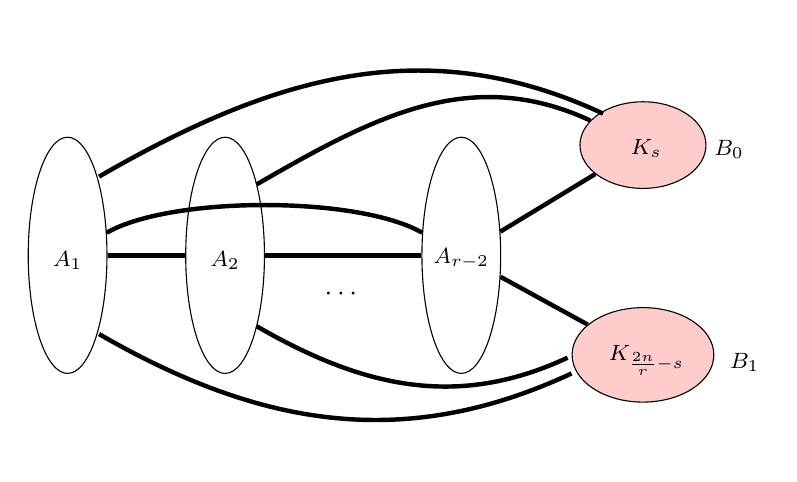
\begin{tikzpicture}[
    node distance=1.5cm,
    set/.style={ellipse, draw, minimum width=1cm, minimum height=3cm},
    smallset/.style={ellipse, draw, minimum width=1.8cm, minimum height=1.2cm},
    ssmallset/.style={ellipse, draw, minimum width=1.6cm, minimum height=1.1cm},
    label/.style={above, font=\footnotesize},
]

% 绘制 A_i 集合 (r-2个)
\foreach \i in {1,...,2} {
    \node[set, fill=blue!0] (A\i) at (\i*2,0) {};
    \node[label] at (\i*2,-0.3) {$A_\i$};
}
\node at (5.5,-0.5) {$\cdots$};
\node[set, fill=blue!0] (A3) at (7,0) {};
\node[label] at (7,-0.3) {$A_{r-2}$};
\draw[-, ultra thick, black] (A1) 
    to[out=30, in=150, looseness=0.6] 
    node[above, pos=0.5] {} (A3);
% 绘制 B_0 和 B_1 集合
\node[ssmallset, fill=red!20, right=of A3] at (7,1.4) (B0) {};
\node[label] at (9.35,1.12) {$K_s$};
\node[label] at (10.4,1.1) {$B_0$};

\node[smallset, fill=red!20, below=of B0] (B1) {};
\node[label] at (9.35,-1.65) {$K_{\frac{2n}{r}-s}$};
\node[label] at (10.6,-1.6) {$B_1$};

\draw[ultra thick,black] (A1)--(A2);
\draw[ultra thick,black] (A2)--(A3);
\draw[ultra thick,black] (A3)--(B0);
\draw[ultra thick,black] (B1)--(A3);
\draw[-, ultra thick, black] (4.4,0.9) 
    to[out=30, in=155, looseness=1] 
    node[above, pos=0.5] {} (B0);
\draw[-, ultra thick, black] (4.4,-0.9) 
    to[out=-30, in=-155, looseness=1] 
    node[below, pos=0.5] {} (8.35,-1.3);
\draw[-, ultra thick, black] (2.4,1) 
    to[out=30, in=155, looseness=1] 
    node[above, pos=0.5] {} (8.8,1.8);
\draw[-, ultra thick, black] (2.4,-1) 
    to[out=-30, in=-155, looseness=1] 
    node[below, pos=0.5] {} (8.4,-1.5);

% 绘制边集表示
%\draw[->, thick] (A1) -- ++(0,2) node[above] {$\{uv:u\in A_i, v\notin A_i\}$};
%\draw[->, thick] (B0) -- (B1) node[midway, right] {$\{uv:u\in B_j, v\notin B_{j+1}\}$};

% 添加省略号表示更多A_i集合

%\node at (5.5,-1.5) {$\cdots$};

% 添加图例


\end{tikzpicture}
    \caption{(EX2). Each thick line indicates that all possible edges exist between the two corresponding parts.}
    \label{fig:extremal}
\end{figure}


Define $\sigma(G):=\min \left\{d(x)+d(y): x,y\in V(G) \ \text{and} \ xy\notin E(G)\right\}$. Hence the condition  $d(x)+d(y)\leq 2k$ for every edge $xy\in E(G)$ is equivalent to $\sigma(G)\geq 2(n-k)-2$. Having established the above, we now only need to prove the following result, as Theorem~\ref{mainore}  follows directly by considering the complement graph. %Therefore, to prove Theorem~\ref{mainore}, it suffices to establish the following result. 
\begin{theorem}\label{FVersion}
    Let $r$ be a positive integer. There exists an integer $n_0:=n_0(r)$ such that the following holds for every integer $n\geq n_0$ with $r\mid n$. Let $G$ be an $n$-vertex graph with $\sigma(G)\geq 2(1-\frac{1}{r})n-2$. Then either $G$ admits a $K_r$-factor or $G$ is extremal. Moreover, there
is an algorithm with polynomial time 
that decides whether $G$ has a $K_r$-factor. 
\end{theorem}


%or this problem, we just need to consider the case $r\mid n$. For the case $r\nmid n$, we can transform it to the former by adding isolated vertices. Let us consider the complement graph $\overline G$ of $G$. Find an equitable $r$-coloring of $G$ is equal to find a $K_{\frac{n}{r}}$-factor of $\overline{G}$. We can get the following theorem.

%\begin{theorem}\label{FVersion}
%    For any positive integer $r$, there exists  $n_0=n_0(r)$ and $n\ge n_0$ with $r\mid n$, If a $n$-vertex $G$ with $\sigma (G)\ge 2(1-\frac{1}{r})n-2$, then $G$ has a $K_r$-factor or $G$ is one of extremal graphs.
%\end{theorem}



 %The $\frac{n}{r}$-extremal graph and $\frac{n}{r}+1$-extremal graph are our extremal graphs.

% To conclude this subsection, we give a quick proof of Theorem \ref{mainore} by combining Theorem \ref{FVersion} with an approach inspired by Larman's method in \cite{La1969}.

% %We end this subsection by giving a quick proof of Theorem \ref{mainore} by using Theorem \ref{FVersion} and a similar idea from Larman \cite{La1969}. %, we can prove Theorem \ref{mainore}.

% \begin{proof}[\bf Proof of Theorem \ref{mainore}]
%    Given integers $k,\,n$ and a constant $c$ such that  $0<\frac{c}{k}<\frac{1}{n}\ll 1$. % with $0< \frac{1}{n}<\frac{1}{k}\ll 1$. % positive integer $r$, we choose a constant $c$ such that 
%    %$$
%    %\frac{1}{n}\ll \frac{1}{r}\le c\le \frac {1}{r-1}.
%    %$$
%    Let $G$ be an $n$-vertex graph where every edge $xy\in E(G)$ satisfies $d(x)+d(y)\le 2k$, and 
% $G$ admits no equitable $k$-coloring. %Let $G$ be an $n$-vertex graph satisfying $d(x)+d(y)\le 2k$ for every edge $xy\in E(G)$ and $G$ has no equitable $k$-coloring $n:=|G|\ge n_0(r)$ following Theorem \ref{FVersion}. Suppose that $G$ is as in the statement of Theorem \ref{mainore}. 
% Assume that $n\equiv q \pmod{k}$, where  $0\le q \le k-1$. %, where $r,q\in \mathbb{N}$ and $0\le q \le k-1$, then set 
% Define $G':= G\cup K_q$ and $r:=\frac{|G'|}{k}$. Then $k \mid |G'|$, $d(x)+d(y)\le 2k$ for each edge $xy\in E(G')$, and the restriction of any equitable $k$-coloring of $G'$ to $G$ is also an  equitable $k$-coloring of $G$. 

%     Denote by $\overline{G'}$ the complement graph of $G'$. Observe that 
%     $$
%     \sigma(\overline{G'})\ge 2|G'|-2-2k=\left(1-\frac{1}{r}\right)|G'|-2.
%     $$
%     Since $\frac{c}{k}<\frac{1}{n}$, one has $r<\frac{1}{c}$. It follows from Theorem \ref{FVersion} that  $\overline{G'}$ has a $K_r$-factor unless $\overline{G'}$ is one of the extremal graphs. If {\rm (EX1)} holds, then  $G'$ contains $K_{k+1}$ as a subgraph. Recall that $G'=G\cup K_q$. Hence, there exists a copy of $K_{k+1}$ in $G$. Similarly, if {\rm (EX2)} holds, then $G$ has a copy of $K_{s,2k-s}$ for some positive  odd integer $s\le k$, as desired.
%     %$\overline{G'}$ is a copy of a graph in (EX1), then there $G'$ contains $K_{k+1}$ as a subgraph. Recall that $G'=G\cup K_q$. Hence, there exists a copy of $K_{k+1}$ in $G$. If $\overline{G'}$ is a copy of a graph in (EX2), then $G$ contains a subgraph $K_{s,2k-s}$ where $s$ is odd and $0<s\le k$. It follows from the fact that $G'=G\cup K_q$ that $G$ has a copy of $K_{s,2k-s} $, as desired.
% \end{proof}

\subsection{Sketch of the proof of Theorem \ref{FVersion}}

%For $r=1$, it is trivial. For $r=2$, we obtain the results by analyzing the structure of $G$. 
Suppose that $r\ge 3$. Given $\gamma>0$ and  a vertex subset $S\subseteq V(G)$, we say $S$ is a $\gamma$-\textit{independent set} of an $n$-vertex graph $G$ if $|E(G[S])|\leq \gamma n^2$. Let $G$ be an $n$-vertex graph with $\sigma(G)\geq 2(1-\frac{1}{r})n-2$. We divide the proof of Theorem \ref{FVersion} into two parts according to $G$ contains a $\gamma$-independent set of size $\frac{n}{r}$ (extremal case) or not (non-extremal case). 

\medskip
\textbf{Non-extremal case: $G$ contains no $\gamma$-independent sets of size $\frac{n}{r}$.}
\medskip

For the non-extremal case, our proof primarily adopts the framework of the absorption method proposed by R\"odl, Ruci\'nski and Szemer\'edi~\cite{RRS2009}, which provides an efficient framework for constructing spanning subgraphs.
The absorption method typically decomposes the problem of finding perfect tilings into two steps. First, one constructs a `small' absorbing set $M$ in the host graph $G$, which can `absorb' any small set of `remaining' vertices. The second step is to find an almost perfect $K_r$-tiling covering almost all vertices in $G-M$.

{\bf Absorbing.} 
We are to find a `small'
$K_r$-absorbing set $M$ in $G$ that absorbs any `very small' set of vertices in $G$. To prove that such a $K_r$-absorbing set $M$ exists, we refine  the widely used method by R\"odl, Ruci\'nski, and Szemer\'edi~\cite{RRS2009} and H\`an, Person, and Schacht  \cite{Han2009}. That is, we show that
%we show that it is sufficient that 
$$
\textit{almost all}\ r\text{-subset}\ T\subseteq V(G)\ \text{has}\  \Omega(n^{r^2})\ K_r\text{-absorbers for}\ T.
$$
%This relaxes the condition in the widely used method by R\"odl, Ruci\'nski, and Szemer\'edi~\cite{RRS2009} and H\`an, Person, and Schacht  \cite{Han2009}, which requires the condition to hold for all $r$-subsets.



%To prove that such an $K_r$-absorbing set $M$ exists, we modify the widely used method by R\"odl, Ruci\'nski, and Szemer\'edi~\cite{RRS2009} and H\`an, Person, and Schacht  \cite{Han2009}. That is, it is sufficient to show that
%$$
%\textit{almost all}\ r\text{-subset}\ T\subseteq V(G)\ \text{has}\  \Omega(n^{r^2})\ K_r\text{-absorbers for}\ T.
%$$
%which relax the condition to prove it holds for all $r$-subset.
 
{\bf Almost cover.} 
 We apply the Regularity Lemma to $G$ and thus obtain a reduced graph $R$ that inherits the Ore's condition of $G$. Our goal is to find an almost perfect $K_r$-tiling of $R$. We begin by greedily selecting a maximal family of vertex-disjoint $K_r$ copies in $G$. % First, we greedily  select a maximal collection of vertex-disjoint $K_r$ copies in $G$. 
 Then, for each 
$s=r-1,r-2,\ldots,1$ in descending order, we iteratively maximize the number of vertex-disjoint $K_s$-copies in the remaining graph. This process constructs  a maximum $(K_r,K_{r-1},\ldots,K_1)$-factor in $R$ (see Definition \ref{maximum-factor}). 

Suppose that $R$ contains no almost perfect $K_r$-tiling. Assume the largest
$K_r$-tiling in $R$ covers exactly  $q\leq (1-o(1))|R|$  vertices. We then prove that the blow-up graph  $R[2^{r-1}]$ admits a maximum $(K_r, K_{r-1}, \ldots, K_1)$-factor covering significantly more than $q \cdot 2^{r-1}$ vertices. 
%Then, we show that there is a maximum $(K_r,K_{r-1},\ldots,K_1)$-factor in $R[2^{r-1}]$ (the bolw-up of $R$) covering substantially more than $d2^{r-1}$ vertices. 
Thus,
crucially, the largest $K_r$-tiling in $R[2^{r-1}]$ covers a larger proportion of vertices than that in $R$. By repeating this process, we obtain a blow-up graph $R'$ of $R$ that
contains an almost perfect $K_r$-tiling.  Our approach adapts a proof technique of Treglown \cite{Treg2016}, developed for finding $K_r$-factors under a degree sequence condition.%we greedily choose a maximal family of vertex-disjoint $K_{r-1}$ copies, followed by a maximal family of $K_{r-2},\ldots,k_1$ copies in what remains. That is, we 

\medskip
\textbf{ Extremal case: $G$ contains a $\gamma$-independent set of size $\frac{n}{r}$.}
\medskip



 
 


%given any $r$-subset $T$ in $V(G)$, there are `many' $r^2$-sets $X\subseteq V(G)$ so that both $G[X]$ and  $G[X\cup T]$ contain perfect $K_r$-tilings.


For the extremal case, we will make use of a result %by Gan, Han, and Hu 
concerning $K_r$-factors in balanced $r$-partite graphs (Lemma~ \ref{GHH2024}) as well as the Graph Removal Lemma  (Lemma~\ref{GRL}). 
Define $S:=\{v:\in V(G):d(x)<(1-\frac{1}{r})n-1\}$. Clearly, $G[S]$ is a clique by Ore's condition. Since $G$ has a $\gamma$-independent set of size $\frac{n}{r}$, one may construct a \textit{good partition} $\mathcal{Q}=\{A_1,A_2,\ldots,A_s,B\}$ of $V(G)$ (see Definition~\ref{Partition}) such that each $|A_i|=\frac{n}{r}$ and $S\subseteq B$, where each $A_i$ is an almost independent set while $G[B]$ has no $\gamma$-independent set of size $\frac{n}{r}$. %In particular, through appropriate modifications, the partition $\mathcal{Q}$ can be transformed into a good partition of 

Under the partition $\mathcal{Q}$, the process of using Lemma~\ref{GHH2024} to construct a $K_r$-factor in $G$ consists of the following two steps:

Step 1. Cover all non-excellent vertices (i.e., those failing the minimum degree condition) using vertex-disjoint $K_r$ copies. To achieve this, we first identify a small structural `base' that covers all such vertices. This base is selected with extension properties that guarantee it can be extended into a $K_r$-tiling while maintaining the original vertex proportion across all parts. Denote the resulting $K_r$-tiling obtained in this step by $\mathcal{T}$. 

Step 2. Find a $K_{r-s}$-tiling in $G[B\setminus V(\mathcal{T})]$. For $r-s\geq 3$, such a $K_{r-s}$-tiling can be obtained by using the non-extremal case. Now, suppose that $r-s=2$ and $G[B\setminus V(\mathcal{T})]$ contains no perfect matching. Assume that $G$ is not extremal.  Proposition \ref{PMatching} implies that $G[B\setminus V(\mathcal{T})]$ consists of two odd components. 
By using some structure analysis, we can perform  minor adjustments to the bases obtained in Step 1 to construct a new $K_r$-tiling $\mathcal{T}'$ that covers all non-excellent vertices and $G[B\setminus V(\mathcal{T}')]$ contains a perfect matching.

After the above steps, we contract each $K_{r-s}$ copy in the $K_{r-s}$-tiling of  $G[B\setminus V(\mathcal{T})]$ into a single vertex. This allows us to apply Lemma~\ref{GHH2024} to obtain a $K_{s+1}$-factor in the remaining graph, which in turn yields a $K_r$-factor in the graph $G- V(\mathcal{T}')$. Combining this with $\mathcal{T}$ or $\mathcal{T}'$ yields the desired $K_r$-factor in $G$.


\subsection{Organization}
In Section \ref{section2}, we present some preliminaries and results on matchings in graphs. Section~3 is devoted to the proof of Theorem~\ref{FVersion}, which is divided into two parts: the non-extremal case (Theorem~\ref{non-extremal}) and the extremal case (Theorem~\ref{Extremal case}). The non-extremal case is proved in Section~\ref{section4} by using the almost cover lemma (Lemma~\ref{almost-cover}, proved in Section \ref{section4.2}) and the absorbing lemma (Lemma~\ref{absorbing}, proved in Section \ref{section4.3}). Section~\ref{section5} deals with the extremal case and provides a proof of Theorem~\ref{Extremal case}. The proof consists of two main steps: constructing a good partition of $G$ (Lemma~\ref{Lpartition}, proved in Section~\ref{section6}) and covering all non-excellent vertices (Lemma~\ref{K_r-tiling}, proved in Section~\ref{section7}). In the last section, we show that there
is an algorithm with polynomial time 
that decides whether $G$ has a $K_r$-factor, and some concluding remarks are also given in this  section. 




\section{Notation and Preliminaries}\label{section2}



\subsection{Notation}
Throughout the paper we follow the standard graph-theoretic notation~\cite{diestel2017graph}. Let $G=(V(G),E(G))$ be a  graph, where $V(G)$ and $E(G)$ are the vertex set and edge set of $G$, respectively.
The \textit{order} of a graph $G$, denoted by $|G|$, is the  number of vertices, and its \textit{size}, denoted by $e(G)$, is the  number of edges.   %The number of vertices of a graph $G$ is denoted by $|G|$, and its number of edges is denoted by $e(G)$. 
Let $U\subseteq V(G)$ be a vertex subset. Denote by $G[U]$ the induced 
subgraph of $G$ on $U$. The notation $G-U$ is used to denote the induced subgraph after removing $U$,
that is $G-U:=G[V(G)\setminus U]$. Given two vertex subsets $A,B\subseteq V(G)$, we use $G[A,B]$ to denote the subgraph of $G$ with vertex set $A\cup B$ and edge set consisting of all edges having one endpoint in $A$ and the other in $B$. For a family $\mathcal{G}$ of graphs, denote by $|\mathcal{G}|$ the number of graphs in $\mathcal{G}$, and let $V(\mathcal{G}) = \bigcup_{G \in \mathcal{G}} V(G)$.

The \textit{neighborhood} of a vertex $v$ in a graph $G$, denoted $N_G(v)$, is the set of all vertices adjacent to $v$. The \textit{degree} of $v$ in $G$, denoted $d_G(v)$, is the number of vertices in $N_G(v)$; when there is no ambiguity, we abbreviate these as $N(v)$ or $d(v)$.  For two vertex subsets $S, A \subseteq V(G)$, denote  $N(S):=\bigcap_{v\in S}N(v)$, $N(v, A):=N(v)\cap A$ and $N(S, A):=N(S)\cap A$, % be the abbreviation of $N(v)\cap A$ and $N(S)\cap A$, respectively. 
 and denote by $d(v,A), d(S)$ and $d(S,A)$ the sizes of $N(v,A),N(S)$, and $N(S,A)$, respectively. When $A$ is a subgraph of $G$, we always abbreviate $V(A)$ as $A$ in the notations above.  Let $\delta(G):=\min\{d(v):v\in V(G)\}$ and $\Delta(G):=\max \{d(v):v\in V(G)\}$ be the \textit{minimum degree} and \textit{maximum degree} of $G$ respectively.   

A \textit{partition} of $V(G)$ is a family $\mathcal{P}=\{A_1,\ldots,A_s\}$ of disjoint subsets satisfying $V(G)=\bigcup_{i=1}^s A_i$. Given two graphs $H$ and $G$, an  \textit{$H$-tiling} of $G$ is a collection of vertex-disjoint copies of $H$ in the graph $G$. A \textit{perfect $H$-tiling} of $G$, or an \textit{$H$-factor}, is an $H$-tiling that covers all vertices of $G$. %Let $V(\mathcal{T})$ be the union of the vertex set of the subgraph $H\in \mathcal{T}$. 
A \textit{matching} in a graph is a set of edges such that no two edges share a common vertex. A \textit{maximum matching} is a matching that contains the largest possible number of edges. We call a matching $M$ of $G$ a \textit{$d$-matching} if $e(M)=d$.


%We say a $K_2$-tiling of $G$ is a \textit{matching} of $G$. A matching $M$ of $G$ is \textit{maximum} if $|M|\ge |M'|$ for every matching $M'$ in $G$. Furthermore, we call a matching $M$ of $G$ a \textit{$d$-matching} if $|M|=d$.

Consider a graph $F$ and an integer $t\in \mathbb{N}$. Let $F[t]$ denote the graph obtained from $F$ by replacing every vertex of $F$ 
 with an independent set of size $t$, and connecting two vertices from different sets if and only if their original vertices are adjacent in $F$. %vertex $x\in V(F)$ by $t$ independent vertices, and joining two vertices in $F[t]$ if and only if the two original vertices are adjacent in $F$.
%each $u\in U_x$ to each $v\in U_y$ precisely when $xy$ is an edge in $F$. 
We will refer to $F[t]$ as a \textit{blow-up} copy of $F$. 
The \textit{join} of two vertex-disjoint graphs $G_1$ and $G_2$, denoted $G_1\vee G_2$, is formed by taking their disjoint union and then adding every possible edge between vertices of $G_1$ and vertices of $G_2$. 
 
%For two vertex-disjoint graphs $G_1=(V_1,E_1)$ and $G_2=(V_2,E_2)$, the \textit{join} of $G_1$ and $G_2$, denoted $G_1\vee G_2$, is a graph with vertex set $V_1\cup V_2$ and edge set $E_1\cup E_2 \cup\{xy:x\in V_1,y\in V_2\}$. 

Given a set $U$ 
and an integer $k$, we write
$\binom{U}{k}$ the collection of all 
$k$-element subsets of $U$. For any integers $a\leq b$, define $[a,b]:=\{i\in \mathbb{N}:a\leq i\leq b\}$ and $[b]:=[1,b]$. When we write  $\alpha\ll \beta\ll \gamma$, we always mean that $\alpha, \beta, \gamma$  are constants in $(0,1)$; and $\alpha\ll \beta$ means that there exists $\alpha_0=\alpha_0(\beta)$ such that the subsequent arguments hold for all $0<\alpha\leq \alpha_0$. Hierarchies of other lengths are defined analogously.

\subsection{Preliminaries}

In this subsection, we will give some preliminary results that will be used in our proof. The following fact from Ore's condition will be used throughout this paper. 

\begin{fact}\label{clique}
   Let $t$ be a positive integer. Assume that $G$ is an  $n$-vertex graph with $\sigma(G)\ge t$. Define $S:=\{x\in V(G): d(x)<\frac{t}{2}\}$. Then $G[S]$ is a complete graph.
\end{fact}



%\begin{proposition}\label{Independentset}
%Choose positive integers $n,\,r$ and a constant $\alpha$ satisfying $r\geq 3$ and $\frac{1}{n}\ll \alpha \ll \frac{1}{r}$. Suppose that $G$ is a graph on $n$ vertices such that 
%\begin{align}\label{OreInKfree}
%\sigma(G)\ge 2\left(1-\frac{1}{r-1}-\alpha\right)n.
%\end{align}
%If $G$ is $K_r$-free, then $G$ contains an independent set of size at least $\left(\frac{1}{r-1}-(r-1)\alpha\right)n$.
%\end{proposition}

%\begin{proof}
%    Let $S:=\{v\in V(G):~d(v)< (1-\frac{1}{r-1}-\alpha)n\}$ and $G':= G-S$. Fact \ref{clique} indicates that $G[S]$ is a clique. Since $G$ is $K_r$-free, we have $|S|\le r-1$.  Then 
%\begin{align}\label{MinKfree}
%\delta(G')\ge \left(1-\frac{1}{r-1}-\alpha\right)n-|S|\ge \left(1-\frac{1}{r-1}-\alpha\right)|G'|-r.
%\end{align} 
%Thus, by the Hajnal-Szemer\'{e}di Theorem, for each vertex $v\in V(G')$, there exists a copy of $K_{r-2}$, say $K^v$, such that $v\in V(K^v)$. %Let $N_{com}(K)$ denote the common neighbors of $V(K)$. 
%It follows from \eqref{MinKfree} that 
%$$
%\Big|\bigcap_{w\in V(K^v)}N(w)\Big|\ge \left(1-\frac{r-2}{r-1}-(r-2)\alpha\right)|G'|-r(r-2)\ge \left(\frac{1}{r-1}-(r-1) \alpha\right)n.
%$$
%Since $G$ is $K_r$-free, we obtain that $\bigcap_{w\in V(K^v)}N(w)$ is an independent set of size at least  $(\frac{1}{r-1}-(r-1)\alpha)n$ in $G$, as desired.
%\end{proof}

We next recall the definition of $\gamma$-independent set.  Given an $n$-vertex graph $G$ and a constant $\gamma > 0$, we define a vertex subset $S \subseteq V(G)$ as a $\gamma$-\textit{independent set} if $e(G[S])\leq \gamma n^2$. 
%{Given $\gamma>0$ and  a vertex subset $S\subseteq V(G)$, we say $S$ is a $\gamma$-\textit{independent set} of an $n$-vertex graph $G$ if $|E(G[S])|\leq \gamma n^2$.} 
Now, we will use the following graph removal lemma to construct a large $\gamma$-{independent set} in graphs. 
\begin{lemma}[Graph Removal Lemma \cite{ADLR1994}]\label{GRL}

For any graph $H$ with $h$ vertices and any $\eps>0$, there exists $\delta>0$ such that any graph on $n$ vertices which contains at most $\delta n^h$ copies of $H$ can be made $H$-free by removing at most $\eps n^2$ edges.
    %Let $\gamma \ge 0$ and $t\in \mathbb{N}$. Given any graph $H$ on $t$ vertices, there exists a constant $\alpha=\alpha(H,\gamma)\ge 0$ and an integer $n_0 =n_0(H,\gamma)$ such that the following holds for all $n\geq n_0$. Suppose that $G$ is a graph on $n$ vertices such that $G$ contains at most $\alpha n^t$ copies of $H$. Then $G$ can be made $H$-free by deleting at most $\gamma n^2$ edges. 
\end{lemma}



\begin{proposition}\label{SuperT}
    Let $0< {1}/{n} \ll \eps \ll \alpha \ll {1}/{r}$ where $r\in \mathbb{N}$ and $r\ge 2$. Suppose that $G$ is an $n$-vertex graph that contains at most $\eps n^r$ copies of $K_r$ and 
$$\sigma(G)\ge 2\Big(1-\frac{1}{r-1}-\alpha\Big)n.$$
%and so that $G$ contains at most $\eps n^r$ copies of $K_r$. 
Then $G$ admits a $\sqrt{\alpha}$-independent set of size at least $\frac{n}{r-1}$.
\end{proposition}

\begin{proof}
    Choose constants satisfying 
    $$\frac{1}{n} \ll \eps\ll \gamma \ll \alpha \ll \frac{1}{r},
    $$
    %Define an addition constant $\gamma$ so that $\eps\ll \gamma \ll \alpha$. 
    let $G$ be a graph as in the assumption. The result is trivial when $r=2$ as $\eps\ll \alpha$. Thus, one may assume that $r\ge 3$. %same as the statement of the proposition. 
    Since $G$ contains at most $\eps n^r$ copies of $K_r$, Lemma~\ref{GRL} implies that one can remove at most $\gamma n^2$ edges from $G$ to obtain a spanning subgraph $G'$ that is $K_r$-free. 
    Define
    $$
    L:=\left\{v\in V(G):d_G(v)-d_{G'}(v)>2\sqrt{\gamma}n\right\}\ \text{and}\ G'':=G'-L.
    $$
    %Let $L$ be a vertex subset consisting of all vertices that are incident to more than $2\sqrt{\gamma}n$ edges in $E(G)\setminus E(G')$ and let $G''=G-L$. 
    Clearly, $|L|\leq \sqrt{\gamma}n$. 
    %Hence, there are at most $\sqrt{\gamma}n$ vertices in $G$ are incident to more than $2\sqrt{\gamma}n$ edges in $E(G)\setminus E(G')$. 
    Since $\gamma\ll \alpha$, %there exists an induced subgraph $G''$ of $G'$ such that 
    one has 
    $$
    n'':=|G''|\ge (1-\alpha)n,\ \text{and}\ \sigma(G'')\ge 2\Big(1-\frac{1}{r-1}-2\alpha\Big)n''.
    $$ %(Actually, we delete all vertices whose reduce more that $2\sqrt{\gamma}n$ neighbors from $G$ to $G'$.)
    %Recall that $G''$ is $K_r$-free.  
    \begin{claim}\label{Independentset}
        The graph $G''$ contains an independent set $S$ of size at least 
$\big(\frac{1}{r-1}-3r \alpha\big)n.$
    \end{claim}
    \begin{proof}[Proof of Claim \ref{Independentset}]
        Let $S:=\left\{v\in V(G''):~d(v)< (1-\frac{1}{r-1}-2\alpha)n''\right\}$ and $\Tilde{G}:= G''-S$. Fact \ref{clique} indicates that $G''[S]$ is a clique. Notice that $G''$ is $K_r$-free, we have $|S|\le r-1$.  Then 
\begin{align}\label{MinKfree}
\delta(\Tilde{G})\ge \Big(1-\frac{1}{r-1}-2\alpha\Big)n''-|S|\ge \Big(1-\frac{1}{r-1}-2\alpha\Big)|\Tilde{G}|-r.
\end{align} 
Thus, by Theorem \ref{KK2008} (or by  Hajnal-Szemer\'{e}di Theorem), for each vertex $v\in V(\Tilde{G})$, there exists a copy of $K_{r-2}$  containing $v$ in $\Tilde{G}$, say $K^v$. %Let $N_{com}(K)$ denote the common neighbors of $V(K)$. 
It follows from \eqref{MinKfree} that 
\begin{align*}
\Big|\bigcap_{w\in V(K^v)}N_{\Tilde{G}}(w)\Big|&\ge \left(1-\frac{r-2}{r-1}-2(r-2)\alpha\right)|\Tilde{G}|-r(r-2)\\
&\ge \left(\frac{1}{r-1}-2(r-1) \alpha\right)n\ge \left(\frac{1}{r-1}-3r \alpha\right)n.
\end{align*}
Since $G''$ is $K_r$-free, we obtain that $\bigcap_{w\in V(K^v)}N_{G''}(w)$ is an independent set of size at least  $\big(\frac{1}{r-1}-3r \alpha\big)n$ in $G''$, as desired.
    \end{proof}
    
    
    
    %Claim \ref{Independentset} implies that $G''$ contains 
    
    Let $S$ be an independent set of size at least 
$\big(\frac{1}{r-1}-3r \alpha\big)n$ in $G''$. 
The construction of $G''$ ensures that $S$ is a $\gamma$-independent set in $G$. By augmenting $S$ with at most $3r\alpha n$ additional vertices, we obtain a $\sqrt{\alpha}$-independent set in $G$ of size at least $\frac{n}{r-1}$, as required.
\end{proof}

%In paper \cite{GHH2024}, Gan, Han, and Hu show the following lemma.

The following theorem provides a degree condition that guarantees the existence of $K_r$-factors in a balanced $r$-partite graph, which follows from \cite[Lemma 6.3]{GHH2024} by using Edmonds algorithm. 
\begin{lemma}[\cite{GHH2024}]\label{GHH2024} 
For any $r,n\in \mathbb{N}$, let $G$ be an $r$-partite graph on vertex classes $V_1,\ldots,V_r$ where $|V_i|=n$ for each $1\le i\le r$. If  
$$
\min_{i\in [r]}\min_{v\in V_i}\min_{j\in [r]\setminus \{i\}} |N(v)\cap V_j|\geq \Big(1-\frac{1}{2r}\Big)n,
$$
%$$d(x,A_j) \ge (1-\frac{1}{r})n+1$$ where $x\in A_i$ and $i\ne j$, 
then in time $O(rn^4)$ we can find a $K_r$-factor of $G$.
\end{lemma}

We will use the following version of Chernoff's bound.
\begin{lemma}\label{chernoff}
    Let $X$ be a random variable with binomial or hypergeometric distribution, and let $0<\eps<\frac{3}{2}$. Then 
    $$
    \mathbb{P}[|X-\mathbb{E}(X)|\geq \eps \mathbb{E}(X)]\leq 2e^{-\frac{\eps^2}{3}\mathbb{E}(X)}.
      $$
\end{lemma}


\subsection{Matchings in graphs}
%section 2,5 放到一起？
%The following are some tools we will use to prove the extremal case.
In this subsection, we  introduce some preliminaries that are related to matchings in graphs. 
\begin{lemma}[\cite{Treg2015}]\label{matching}
    Let $d,n \in \mathbb{N}$. Suppose that $G$ is a graph on $n\ge 2d$ vertices with  $\delta(G)\ge d$. Let $X\subseteq V(G)$ be a subset of size $d$.  Then $G$ contains a $d$-matching that covers all vertices in $X$. 
\end{lemma}
Let $M$ be a maximum matching of a graph $G$ and $v$ be a vertex in $V(G)\setminus V(M)$, define 
$$
SN(v):=\{z\in V(M):wz\in E(M) \text{ for some } w\in N(v)\}.
$$
The following fact follows immediately from the definition of a maximum matching; the proof is omitted.  
\begin{fact}\label{MMProperty}
   Let $M$ be a maximum matching of a graph $G$ and $x,y$ be two distinct vertices in $V(G)\setminus V(M)$. %For any vertex $v\in V(G)\setminus V(M)$, define $SN(v):=\{z\in V(M):wz\in M \text{ for some } w\in N(v)\}$. 
   Then $E(G[SN(x),SN(y)])=\emptyset$. %({\color{red}define SN(v) in Notation?}) %  If $M$ is the maximum matching of $G$, then, for any two different vertices $x,y\in V(G)\setminus V(M)$, we have that $E(SN(x),SN(y))=\emptyset$, where $SN(v):=\{z\in V(M):wz\in M \text{ for some } w\in N(v)\}$ for any $v\in V(G)\setminus V(M)$.
\end{fact}

%\begin{proof}[\bf Proof]
    %Suppose for a contradiction that there is an edge $zz'\in E(G)$ such that $z\in SN(x)$ and $z'\in SN(y)$. If $zz'\in M$, then by definition of $SN(x)$ and $SN(y)$, $xz',yz\in E(G)$. Let $M':=(M\setminus \{zz'\})\cup \{xz',yz\}\subseteq E(G)$. Thus, $M'$ is a larger matching than $M$, contradicting the assumption. 
    
    %If $zz'$ is not in $M$, there exist $w,w'$ such that $zw, z'w'\in M$. Define $M:=(M\setminus \{wz,w'z'\})\cup \{xw,zz',w'y\}.$ Thus, $M'$ is a larger matching than $M$, contradicting the assumption.
%\end{proof}

\begin{lemma}\label{MStab}
    Let $d\ge 1$ and $n\ge 3d+2$. Assume that $G$ is an $n$-vertex graph with $d\leq \delta(G)\le \Delta(G)\leq n-2d-1$. Then $G$ admits a matching of size $d+1$. % has a matching $M$ of size at least $d+1$ unless, for any two different vertices $x$ and $y$ in $V(G)\setminus V(M)$, $d(x)=d(y)=d$ and $N(x)=N(y)$.
\end{lemma}

\begin{proof}
   %Suppose to the contrary that $G$ contains no matching of size $d+1$. 
   Choose a maximum matching, say $M,$ inside $G$. Suppose that $e(M)\leq d+1$. Together with Lemma \ref{matching}, we obtain $e(M)=d$.  Let $x_1,x_2,x_3$ be three distinct vertices in $V(G)\setminus V(M)$. Clearly, $N(x_i)\subseteq V(M)$ for each $i\in [3]$.  We are to prove that $N(x_1)=N(x_2)=N(x_3)$. 

   For each $i\in [3]$, assume that there are $a_i$ edges in $M$ such that both endpoints of them are adjacent to $x_i$. If follows from Fact \ref{MMProperty} that $E(SN(x_i),SN(x_j))=\emptyset$ for $1\leq i<j\leq 3$. %By the maximality of $M$, there are no edges in $M$ such that its two endpoints are adjacent to different vertices in $V(G)\setminus V(M)$. 
   Therefore, 
   $d(x_i)\leq 2a_i+d-(a_1+a_2+a_3)$ for each $i\in [3]$. Together with $\delta(G)\geq d$, one has 
   $$
   3d\leq d(x_1)+d(x_2)+d(x_3)\leq 3d-(a_1+a_2+a_3).
   $$
   Hence $a_1=a_2=a_3=0$ and $d(x_1)=d(x_2)=d(x_3)=d$. %That is, each vertex in $V(G)\setminus V(M)$ is adjacent to at most one vertex in each edge of $M$. 
   Consequently, every vertex in $V(G)\setminus V(M)$ is adjacent to exactly one vertex in each edge of $M$. Applying Fact \ref{MMProperty} again yields that every two distinct vertices in $V(G)\setminus V(M)$ share the same neighbors in $V(M)$. Hence each vertex $v\in N(x_1)$ satisfies 
   $
d(v)\geq n-2d
    $, which contradicts the maximum degree  condition of $G$. 
    %It is sufficient to prove that if there is no matching of size $d+1$, $G$ has the above properties. Assume $M$ is the maximum matching with size $d$. Thus, for each $x\notin V(M)$, $N(x)\in V(M)$.  
    %For two different vertices $x$ and $y$ in $V(G)\setminus V(M)$, we have that $d(x)=d(y)=d$. Otherwise, by the pigeonhole principle, there exists an edge $uv\in M$ such that $xu,yv\in E(G)$. Therefore, $M':=(M\setminus \{uv\})\cup\{xu,yv\}$ is a matching of size $d+1$, contradicting the assumption.   
    %Assume that there exist two vertices $x$ and $y$ in $V(G)\setminus V(X)$ such that $N(x)\ne N(y)$. If $N(x)\cap N(y)\ne \emptyset$, then there exists a matching edge $zz'$ such that $z\in SN(x)$ and $z'\in SN(y)$. contradicting Fact \ref{MMProperty}. If $N(x)\cap N(y)=\emptyset$, let $z$ be another vertex in $V(G)\setminus V(M)$. Since $|SN(x)|=|SN(y)|=d$ and $|V(M)|=2d$, we have $SN(z) \subseteq V(M)=SN(x)\cup SN(y),$ that is, there exists an edge $aa'$ such that $aa'\in E(SN(z),SN(x)\cup SN(y))$, contradicting Fact \ref{MMProperty}.
\end{proof}
The main goal of this subsection is to prove the following proposition. 
\begin{proposition}\label{PMatching}
Let $n$ be a positive even integer and $\gamma$ be a constant such that $0<{1}/{n}\ll\gamma\ll 1$. Suppose that $G$ is a graph on $n$ vertices so that 
\begin{align}\label{B2Ore}
\sigma(G)\ge n-\gamma n.
\end{align}
Then one of the following holds:
\begin{itemize}
\setlength{\parskip}{0pt}
    \item[{\rm (i)}] $G$ admits a perfect matching;
    \item[{\rm (ii)}] $G$ contains a $2\gamma$-independent set of size at least $\frac{n}{2}$;
    \item[{\rm (iii)}] $G$ consists of two odd components $C_1$ and $C_2$. Moreover, if $|C_i|\leq \frac{1-\gamma}{2}n$ for some $i\in [2]$, then % the size of a component $C$ is at most $\frac{1-\gamma}{2}n$ then 
    $C_i$ is a clique.
\end{itemize}
\end{proposition}

\begin{proof}
Suppose that $G$ has no perfect matching. Let $M$ be a maximum matching in $G$. Then, $|V(M)|\leq n-2$ and there are two  distinct vertices $x,y\in V(G)\setminus V(M)$. %Define $SN(v):=\{z'\in V(M):zz'\in E(M) \text{ for some } z\in N(v)\}$ for each $v\in V(G)\setminus V(M)$.  
The maximality of $M$ implies that $N(x)\cup  N(y)\subseteq  V(M)$, and so $SN(x)\cup SN(y)\subseteq V(M)$. Since $xy\notin E(G)$,  % For each vertex $x\notin V(M)$, we have that $d(x)=|N(x)|=|SN(x)|$. 
by \eqref{B2Ore} we have 
\begin{align}\label{SNOre}
   d(x)+d(y)= |SN(x)|+|SN(y)|\ge n-\gamma n.
\end{align}
% {\color{red}(delete??)Fact \ref{MMProperty} implies that $E(SN(x),SN(y))=\emptyset$, which also implies $N(x)\cap SN(y)=\emptyset$.  %Since $SN(x)\cup SN(y)\subseteq V(M)$, we have
% Therefore, 
% $$|E(M)|\ge |SN(x)\cap SN(y)|+\frac{|SN(x)\Delta SN(y)|}{2}\ge \frac{n-\gamma n}{2}.$$}
Define $SN(x,y):=SN(x)\cap SN(y)$. Fact \ref{MMProperty} implies that $SN(x,y)$ is an independent set of $G$ and  
\begin{align}\label{degreesum}
    d(x)+d(y)\leq 2e(M)\leq n-2.
\end{align}
We divide our proof into two cases.

\medskip
{\bf Case 1. } 
$SN(x,y)\ne \emptyset$. 
\medskip

In this case, we will show that (ii) holds. 
Without loss of generality, assume that $d(x)\le d(y)$. Then \eqref{degreesum} implies $d(x)<\frac{n}{2}$. Choose $z\in SN(x,y)$ and assume $zz'\in E(M)$. Hence  $z'\in N(x)\cap N(y)$ and  $N(z)\subseteq V(M)$.  Thus, \eqref{B2Ore} implies that 
$$
d(z)\ge n-\gamma n-d(x)>\frac{n}{2}-\gamma n.
$$
Notice that $N(z)\cap (SN(x)\cup SN(y))=\emptyset$. Otherwise, there exists a matching of size $|E(M)|+1$, a contradiction. Thus, 
$|SN(x)\cup SN(y)|\le n-d(z)<\frac{n}{2}+\gamma n$. Together  with \eqref{SNOre}, one has  
$$|SN(x)\cap SN(y)|= |SN(x)|+|SN(y)|-|SN(x)\cup SN(y)|\ge \frac{n}{2}-2\gamma n.$$
Recall that $SN(x,y)$ is an independent set in $G$. By adding at most $2\gamma n$ arbitrary vertices to $SN(x,y)$, we obtain a $2\gamma$-independent set of size at least $\frac{n}{2}$ in $G$, as desired. 



%In this case, we will show that (ii) holds. % $G$ contains a $3\gamma$-independent set of size at least $n/2$. 
%Since $M$ is not a perfect matching, one has $|E(M)|\le \frac{n}{2}-1$. Fact \ref{MMProperty} implies that $N(x)\cap SN(y)=\emptyset$. Moreover, $N(x),SN(y)\subseteq V(M)$. Thus, $|N(x)|+ |SN(y)|\le n-2$. 
%Without loss of generality, assume that $d(x)\le d(y)$. Choose $z\in SN(x,y)$ and assume $zz'\in E(M)$. Hence  $z'\in N(x)\cap N(y)$ and  $N(z)\subseteq V(M)$.  Thus, \eqref{B2Ore} implies that 
%$$
%d(z)\ge n-\gamma n-d(x).
%$$

%If $d(x)\le \frac{n}{2}-2\gamma n$, then $d(z)\geq \frac{n}{2}+\gamma n$. Similarly, \eqref{SNOre} implies $d(y)\ge \frac{n}{2}+\gamma n$. 
%Thus, $d(y)+d(z)\geq n+2\gamma n$, that is, $(N(z)\cap SN(y))\setminus \{z'\}\ne \emptyset$. Assume $w\in (N(z)\cap SN(y))\setminus \{z'\}$ and $ww'\in E(M)$. Then $M':=(M \setminus\{zz',ww'\})\cup \{xz', yw',zw\}$ is a matching of size $|E(M)|+1$, a contradiction. 

%If $d(x)> \frac{n}{2}-2\gamma n$, then by \eqref{degreesum} one has  $d(x)\le \frac{n}{2}\leq d(y)\le \frac{n}{2}+2\gamma n$. Therefore, $d(z)\geq \frac{n}{2}-3\gamma n$. % Consider vertices $x,z$, \eqref{B2Ore} implies that $$d(z)\ge n-\gamma n -d(x) > \frac{n}{2}-\gamma n.$$ 
%Notice that $N(z)\cap (SN(x)\cup SN(y))=\emptyset$. Thus, 
%$|SN(x)\cup SN(y)|\le |V(M)|-d(z)\le \frac{n}{2}+3\gamma n-2$. Together  with \eqref{SNOre}, one has  
%$$|SN(x)\cap SN(y)|= |SN(x)|+|SN(y)|-|SN(x)\cup SN(y)|\ge \frac{n}{2}-4\gamma n.$$
%Recall that $SN(x,y)$ is an independent set in $G$. By adding at most $4\gamma n$ arbitrary vertices to $SN(x,y)$, we obtain a $5\gamma$-independent set of size at least $\frac{n}{2}$ in $G$, as desired. 

\medskip
{\bf Case 2.} %For each maximum matching $M$ and any two vertices $x,y\in V(G)\setminus V(M)$, we have 
$SN(x,y)=\emptyset.$
\medskip

In this case, one may assume that 
$SN(x,y)=\emptyset$ for every maximum matching $M$ of $G$ and any two distinct  vertices $x,y\in V(G)\setminus V(M)$. Suppose that  $|V(G)\setminus V(M)|>2$. Then there is a vertex $z\in V(G)\setminus (V(M)\cup \{x,y\})$. It follows from  \eqref{B2Ore} that 
$$d(x)+d(y)+d(z)\ge \frac{3}{2}(n-\gamma n)>|V(M)|.$$ 
Recall that $N(x)\cup N(y)\cup N(z)\subseteq V(M)$. Therefore, there are two vertices $u,v\in \{x,y,z\}$ such that $N(u)\cap N(v)\neq \emptyset$, thus $SN(u,v)\neq \emptyset$, a contradiction. Hence, $|V(G)\setminus V(M)|=2$. We will show that (iii) holds. 

%, Fact \ref{MMProperty} implies that, for any three different vertices $x_1,x_2,x_3\in  V(G)\setminus V(M)$, we have $$e(G[SN(x_i),SN(x_j)])=0,$$
%where $i,j\in \{1,2,3\}$ and $i\ne j$. \eqref{B2Ore} implies that $$d(x_1)+d(x_2)+d(x_3)\ge \frac{3}{2}(n-\gamma n)>|V(M)|$$, that is, there exists $x_i\ne x_j$ such that $SN(x_i)\cap SN(x_j)\ne \emptyset$, contradicting the assumption.

%If $|V(G)\setminus V(M)|=2$, then d
%Define $R:=V(G)\setminus (SN(x)\cup SN(y)\cup\{x,y\})$. %In fact, one may assume that the maximum matching $M$and vertices $\{x,y\}$ are chosen such that $|R|$ is {\color{red} minimum}. 
%We first consider $R=\emptyset$. Recall that Fact~\ref{MMProperty} implies  $E(G[SN(x),SN(y)])=\emptyset.$ Together with $SN(x,y)=\emptyset$, one may partition the edges in $M$ into two parts, say $M_x\cup M_y$, where $M_x$ denotes the set of edges in $M$ whose both endpoints are adjacent to $x$ and $M_y$ is defined similarly. %It suffices to show that $N(x)\cap SN(y)=\emptyset$ and $N(y)\cap SN(x)=\emptyset$. Indeed, we only need to show the former one. Assume $v\in N(x)\cap SN(y)$, and $vv'\in E(M)$. Then $v'\in SN(x)$, contradicting Fact \ref{MMProperty}.
% If $R=\emptyset$, then by the fact that $SN(x,y)=\emptyset$ 
% and Fact \ref{MMProperty},  %Notice that by replacing  $x$ with any vertex $z\in V(M_x)$, 
% Notice that $G[V(M_x),V(M_y)]$ is an empty graph. Otherwise, suppose that there exists an edge $uv$ such that $u\in V(M_x)$ and $v\in V(M_y)$. Let $uu',vv'\in E(M)$. Hence,  replacing $\{uu',vv'\}$ to $\{xu',uv,v'y\}$ in $M$ obtains a larger matching $M'$, contradicting that matching $M$ is maximum. 
%Therefore, $G[V(M_x)\cup \{x\}]=:C_1$ and $G[V(M_y)\cup \{y\}]=:C_2$ are two connected odd components of $G$, as desired. % forms a clique with odd order. Similarly, $G[V(M_y)\cup \{y\}]$ also forms a clique with odd order, as desired.

%If there exists an edge $uv$ such that $u\in V(M_x)\cup \{x\}$ and $v\in V(M_y)\cup\{y\}$, then replacing $\{uu',vv'\}$ to $\{xu',uv,v'y\}$ in $M$ obtains a larger matching $M'$, contradicting that matching $M$ is maximum.

%{\color{red}By symmetry and the maximality of $|R|$, we obtain that for any vertex $z\in V(M_x)$, it is adjacent to all vertices in $(V(M_x)\cup \{x\})\setminus \{z\}$. Therefore, $G[V(M_x)\cup \{x\}]$ forms a clique with odd order. Similarly, $G[V(M_y)\cup \{y\}]$ also forms a clique with odd order, as desired.}

%Now, we consider $R\neq \emptyset$. 
%Define $R:=V(G)\setminus (SN(x)\cup SN(y)\cup\{x,y\})$. 
Since $SN(x,y)=\emptyset$ and $E(G[SN(x),SN(y)])=\emptyset$, there are two vertex-disjoint subgraphs $G_1:=G[\{x\}\cup SN(x)]$ and $G_2:=G[\{y\}\cup SN(y)]$ in $G$ such that $E(G[V(G_1),V(G_2)])=\emptyset$. Define $R:=V(G)\setminus (V(G_1)\cup V(G_2))$. If $R=\emptyset$, then the two endpoints of each edge in $M$ are adjacent to the same vertex in $\{x, y\}$. It follows that $G$ consists of two connected odd components $G_1$ and $G_2$, as desired. Suppose that $R\neq \emptyset$. In order to prove (iii) holds, it is necessary to assign vertices in $R$ to $G_1$ or $G_2$. Choose a vertex $v \in R$ with $vv'\in E(M)$. Hence $xv',yv'\notin E(G)$. Together with $xy\notin E(G)$ and \eqref{B2Ore}, we have 
%\begin{align*}
%    &d(x)+d(y)=|SN(x)|+|SN(y)|\geq n-\gamma n;\\
%    &d(x)+d(v')=|SN(x)|+|N(v')|\geq n-\gamma n;\\
%    &d(y)+d(v')=|SN(y)|+|N(v')|\geq n-\gamma n.
%\end{align*}
%Therefore,
$$
d(x)+d(y)+d(v')=|SN(x)|+|SN(y)|+|N(v')|\geq \frac{3}{2}(n-\gamma n).
$$
Recall that $SN(x,y)=\emptyset$. Hence, 
\begin{align}\label{eitheror}
    \text{either}\ SN(x)\cap N(v')\ne \emptyset\ \text{or}\ SN(y)\cap N(v')\ne \emptyset.
\end{align}



%By \eqref{B2Ore} and Fact \ref{MMProperty}, we have that
%begin{align}\label{SNproperty}
%    \text{Any vertex $v\in R$ with $vv'\in M$, there is at least a vertex $z\in \{x,y\}$ such that $SN(z)\cap N(z')\ne \emptyset$.}\tag{\ensuremath{*}}
%\end{align} 
$\bullet$\ Assume  $v'\notin R$. Then $v'\in SN(x)\cup SN(y)$. Without loss of generality, assume that $v'\in SN(x)$%and $v'\notin SN(y)$
, that is, $xv\in E(G)$ and $yv\notin E(G)$. Suppose that $N(v)\cap SN(y)\ne \emptyset$. Then choose $u\in N(v)\cap SN(y)$ with $uu'\in E(M)$. Hence $M':=(M\setminus \{vv',uu'\})  \cup \{vu,u'y\}$  is also a maximum matching of $G$. Notice that $v\in N(x)\cap N(v')$. Therefore, under the matching $M'$ we have $SN(x,v')\neq \emptyset$, contradicting our initial assumption in Case 2. Thus, $N(v)\cap SN(y)= \emptyset$. Together with $vy\notin E(G)$, we know $N(v)\cap V(G_2)=\emptyset$. Thus, one may add such a vertex $v$ to $V(G_1)$. % Let us consider vertices $x,v'$, which do not belong to $V(M')$. Thus, we get $u\in SN(x)\cap SN(v')$ in matching $M'$, that is, $SN(x,v')\ne \emptyset$. It is a contradiction. 

$\bullet$\ Assume  $v'\in R$. Then $xv,yv\notin E(G)$. By a similar argument as \eqref{eitheror}, we obtain that
\begin{align}\label{either2}
    \text{either}\ SN(x)\cap N(v)\ne \emptyset\ \text{or}\ SN(y)\cap N(v)\ne \emptyset. 
\end{align}
We claim that 
%$$
%SN(x)\cap (N(v)\cup N(v'))= \emptyset \text{ or }SN(y)\cap (N(v)\cup N(v'))= \emptyset.
%$$
%therwise, one 
none of the following holds:
\begin{enumerate}
    \item[{\rm (1)}] $SN(x)\cap N(v)\ne \emptyset$ and $SN(y)\cap N(v')\neq \emptyset$;
    \item[{\rm (2)}] $SN(x)\cap N(v')\ne\emptyset$ and $SN(y)\cap N(v)\ne \emptyset$. 
\end{enumerate}
%\vspace{-0.2cm}
Otherwise, without loss of generality, suppose the former case happens. Let $a\in SN(x)\cap N(v)$ and $b\in SN(y)\cap N(v')$, and assume  $aa',bb'\in E(M)$. Then $M':=(M\setminus\{aa',bb',vv'\})\cup \{xa',av,v'b,b'y\}$ is a perfect matching of $G$, a contradiction. Together with \eqref{eitheror} and \eqref{either2}, we obtain that 
\begin{align}\label{belong}
    \text{either}\ SN(x)\cap (N(v)\cup N(v'))= \emptyset\ \text{or}\ SN(y)\cap (N(v)\cup N(v'))= \emptyset.
\end{align}
Together with $xv,xv',yv,yv'\notin E(G)$, we have either $(N(v)\cup N(v'))\cap V(G_1)=\emptyset$ or $(N(v)\cup N(v'))\cap V(G_2)=\emptyset$. Therefore, $v$ and $v'$ can be assigned to $G_1$ or $G_2$ based on where their neighbors are located, which preserves the absence of edges between $G_1$ or $G_2$. % based on their neighborhood adjacencies. %Thus, $v,v'$ can be added to $G_1$ or $G_2$ according to their neighbors. 

By sequentially applying the above operation to each vertex in 
$R$, we can assign them to either 
$G_1$ or $G_2$ accordingly. In order to preserve the disconnectivity  between $G_1$ and $G_2$, we only need to show that in the above process, for each edge in $G[R]$, %$uv\in E(G[R])$, $u$ and $v$ 
its two endpoints are assigned to the same part. Let $uv\in E(G[R])$ with $uu',vv'\in E(M)$. We proceed our proof by considering the following three subcases.

%Thus, in order to finish the proof, it suffices to prove that 

%In fact, if the vertex set $R$ forms an independent set in $G$, then $G$ can be partitioned into two connected odd components, as desired. So, in what follows, we consider that there exists an edge $uv\in E(G[R])$, where $uu', vv'\in E(M)$. In order to preserve the disconnectivity  between $G_1$ and $G_2$, we will  show that in the above process, $u$ and $v$ are assigned to the same part.
%$$
%\text{either}\ \big(\bigcup_{w\in \{u,u',v,v'\}}N(w)\big)\cap V(G_1)=\emptyset\ \text{or}\ \big(\bigcup_{w\in \{u,u',v,v'\}}N(w)\big)\cap V(G_2)=\emptyset.
%$$
%. In order to put $u$ and $v$ in suitable parts, it suffices to show that 
%$uu'$ and $vv'$ are not adjacent to vertices in the same part. 


\medskip
{\bf Subcase 2.1.} $u',v'\notin R$.
\medskip

 %we obtain that $N(u)\cap SN(y)=\emptyset$ if $u'\in SN(x)$, and $N(u)\cap SN(x)=\emptyset$ if $u'\in SN(y)$. %Recall that in the above argument, we assumed  $v'\in SN(x)$ and $N(v)\cap SN(y)=\emptyset$. %Hence $vy\notin E(G)$ and $N(v)\setminus \{x\}\subseteq SN(x)\cup R$. 
We claim that there exists a vertex $z\in \{x,y\}$ such that 
$
u',v'\in SN(z).
$ 
Otherwise, suppose that $u'\in SN(x)$ and $v'\in SN(y)$. By the argument in the above,  we obtain that $N(u)\cap SN(y)=\emptyset$ and $N(v)\cap SN(x)=\emptyset$. %, which implies that $uy\in E(G)$ and $ux \notin E(G)$. %We will find a matching $M'$ such that $SN(y)\cap SN(w)\ne \emptyset$ for some vertex $w\in \{u',v'\}$. 
Without loss of generality, assume that $d(x)\le d(y)$. Then $d(x)\le \frac{n}{2}$. It follows from $v\in R$ that $xv'\notin E(G)$. Together with  \eqref{B2Ore} one has $d(v')\geq \frac{(1-2\gamma)n}{2}$. By $v'\in SN(y)$ and Fact~\ref{MMProperty}, we obtain $N(v')\cap SN(x)=\emptyset$. Thus,  $N(v')\subseteq SN(y)\cup R$. Notice that $|R|\leq \gamma n$.  Hence, there exists a vertex $a\in SN(y)\cap N(v')$. Therefore, $M':=(M\setminus \{aa',uu',vv'\})\cup \{uv,v'a,a'y\}$ is also a maximum matching in $G$. But $SN(x,u')\neq \emptyset$, a contradiction. This implies that there exists a vertex $z\in \{x,y\}$ such that 
$
u',v'\in SN(z). 
$
%which further implies $N(v)\cap SN(w)=\emptyset$ and $N(u)\cap SN(w)=\emptyset$, where $w\in \{x,y\}\setminus \{z\}$. 
Therefore, $u$ and $v$ are assigned to the same part by using the above argument. 

%ince $uy\in E(G)$ and $ux \notin E(G)$, then $d(u')\ge \frac{(1-2\gamma)n}{2}$. Since $N(u')\subseteq SN(x)\cup R$ and $|R|\le \gamma n$, then there exists $a'\in SN(x)\cap N(u)$. The matching $M':=(M\setminus \{aa',uu',vv'\})\cap \{uv,u'a,a'x\}$ also is maximum, where $aa'\in M$. The vertices $v',y$ are the vertices we need.

\medskip
{\bf Subcase 2.2.} $u'\in R,\,v'\notin R$.
\medskip

By a similar discussion as Subcase 2.1, we can show that $u$ and $v$ are assigned to the same part. % by using the above argument. $(N(u)\cup N(u'))\cap SN(y)=\emptyset$. %Otherwise, by \eqref{belong} we have $(N(u)\cup N(u'))\cap SN(x)=\emptyset$. 

\medskip
{\bf Subcase 2.3.} $u',v'\in R$.
\medskip

We claim that there exists a vertex $z\in \{x,y\}$ such that 
$$
SN(z)\cap (N(v)\cup N(v'))=\emptyset\ \text{and}\ SN(z)\cap (N(u)\cup N(u'))=\emptyset.
$$ 
Otherwise, based on \eqref{belong}, one may assume that $SN(x)\cap (N(v)\cup N(v'))=\emptyset$ and $SN(y)\cap (N(u)\cup N(u'))=\emptyset$. Furthermore, $SN(y)\cap (N(v)\cup N(v'))\neq \emptyset$ and $SN(x)\cap (N(u)\cup N(u'))\neq \emptyset$. By $uv\in E(G)$ and the maximality of $M$, one has either $SN(y)\cap N(v')=\emptyset$ or $SN(x)\cap N(u')=\emptyset$. 
Assume, without loss of generality, that $SN(y)\cap N(v')=\emptyset$. %Then $SN(y)\cap N(v)\neq \emptyset$ and  $N(v')\subseteq SN(x)\cup R$. 
Together with $SN(x)\cap N(v')=\emptyset$, one has $N(v')\subseteq R$. Notice that  $xv',yv'\notin E(G)$. By  \eqref{B2Ore}, one has $$d(x),d(y)\geq n-2\gamma n,$$
which contradicts \eqref{degreesum}. % If $d(y)\geq d(x)$, then by \eqref{B2Ore} we have $d(v')\geq \frac{(1-2\gamma)n}{2}$. Hence $N(v')\cap SN(x)\neq \emptyset$, a contradiction. Therefore, $d(x)>d(y)$.  
%Choose $a\in SN(y)\cap N(v)$ with $aa'\in E(M)$, and choose $b\in SN(x)\cap (N(u)\cup N(u'))$ with $bb'\in E(M)$.  If $b\in SN(x)\cap N(u')$, then let $M':=(M\setminus \{aa',uu',bb'\})\cup \{xb,b'u',ya'\}$. Notice that under the matching $M'$ we have $SN(u,a)\neq \emptyset$, a contradiction. Hence $SN(x)\cap N(u')=\emptyset$, which implies  $N(u')\subseteq SN(y)\cup R$. Recall that $d(x)\geq d(y)$By Ore condition, we have $d(u')\geq \frac{(1-2\gamma)n}{2}$. Hence $N(u')\cap SN(y)\neq \emptyset$, a contradiction. 

With the above discussion, by assigning vertices in $R$ to $G_1$ or $G_2$ accordingly, we know that $G$ can be decomposed into two connected components, say $C_1$ and $C_2$, each of which has odd order.
%there exists a vertex $z\in \{x,y\}$ such that 
%$$
%SN(z)\cap (\cup_{w\in \{v,v'\}\cap R}N(w))=\emptyset\ \text{and}\ SN(z)\cap (\cup_{w\in \{u,u'\}\cap R}N(w))=\emptyset. 
%$$
%Hence by adding adjacent vertices in the same part, we get two connected components of $G$, each of which has odd order. 
Furthermore, by Ore's condition, if $|C_i|\leq \frac{1-\gamma}{2}n$ for some $i\in [2]$, then $C_i$ is a clique, as desired.
\end{proof}



%Assume that there exists an edge $uu'\in E(M)$ with $u\in R$ and $u'\notin R$. 



%For any two matching edges $vv'$ and $uu'$ with $\{v,u\}\subseteq R$ and $\{v',u'\}\notin R$, if $vu\in E(G)$, then there exists $z\in \{x,y\}$ such that  $$SN(z)\cap N(v)=\emptyset \text{~and~} SN(z)\cap N(u)=\emptyset.$$ Otherwise, there exists another perfect matching $M'$ such that there exists a pair of vertices $z,w$, where $z\in\{x,y\}$ and $w\in \{u',v'\}$, satisfying $SN(z)\cap SN(w)\ne \emptyset$. Without loss of generality, let $d(x)\ge d(y)$, $N(v)\cap SN(x)=\emptyset$, and $N(u)\cap SN(y)=\emptyset$. We have $d(y)\le \frac{n}{2}$.  Since $ux\in E(G)$ and $u'y \notin E(G)$, then $d(u')\ge \frac{(1-2\gamma)n}{2}$. Since $N(u')\subseteq SN(x)\cup R$ and $|R|\le \gamma n$, then there exists $a'\in SN(x)\cap N(u)$. The matching $M':=(M\setminus \{aa',uu',vv'\})\cap \{uv,u'a,a'x\}$ also is maximum, where $aa'\in M$. The vertices $v',y$ are which vertices we need.

% Otherwise,  we claim that 
%$$SN(x)\cap N(v')=\emptyset \text{ or } SN(y) \cap N(v')=\emptyset.$$ 
%Otherwise, without loss of generality, let $v'\in SN(x)$, then $M':=(M\setminus \{vv')\cup\{vx\}$ also is a maximum matching, but $N(v')\cap SN(y)\ne \emptyset$, contradicting the assumption. 



%For any two matching edges $vv'$ and $uu'$ with $\{v,v',u\}\subseteq R$ and $u'\notin R$, if $vu\in E(G)$, then there exists $z\in \{x,y\}$ such that $SN(z)\cap (N(v)\cup SN(v')=\emptyset$ and $SN(z)\cap (N(u)\cup SN(u')=\emptyset$. The proof is similar to $v'\notin R$.

%For any two matching edges $vv'$ and $uu'$ with $\{v,v',u,u'\}\subseteq R$, if $vu\in E(G)$, then there exists $z\in \{x,y\}$ such that $SN(z)\cap (N(v)\cup N(v'))=\emptyset$ and $SN(z)\cap (N(u)\cup N(u'))=\emptyset$. Otherwise, $M$ is not the maximum matching. It is a contradiction. Without loss of generality, let $z\in \{x,y\}$ such that $SN(x)\cap (N(v)\cup N(v'))=\emptyset$ and $SN(y)\cap (N(u)\cup N(u'))=\emptyset$. The condition \eqref{B2Ore} implies that there exists $a,b$ satisfying $a\in SN(x)\cap N(u')$ and $b \in SN(y)\cap N(v')$. Then $M':=(M\setminus \{aa',uu',vv',bb'\})\cup \{xa,a'u',uv,v'b,b'y\}$ is a matching of size $|M'|+1$, where $aa',bb'\in M$.





%Since $u_1u_t\notin E(G)$, $A\subseteq \{u_1,...,u_{t-2}\}$.  Since $|A|+|B|\ge n-2$ and $A\cap B=\emptyset$, if $|P|\le n-2$, then we have $B\subseteq \{u_2,...,u_{t-1}\}\setminus A$ and  $$|\{u_2,...,u_{t-1}\}\setminus A|\le n-4-d(u)+1=n-d(u)-3.$$ It is a contradiction to Ore's condition. It is sufficient to consider $|P|=n-1$. Since $|\{u_1,\dots,u_{t-1}\}\setminus A|\le n-3-d(u)+1=n-d(u)+2$ and $A\cap B=\emptyset$, we have that $d(u_1)+d(u_t)=n-2$.  With loss of generality, let $d(u_1)\ge \frac{n-2}{2}$. If $x\notin V(P)$, then $A \cap N(x)=\emptyset$. Otherwise, 




%Let $SN(u):=\{a_{i-1}:a_i\in N(u)\}$. If $N(v)\cap SN(u)\ne \emptyset$, then there exists a cycle in $G$. By a similar argument for $|P'|<n-2$, $G$ has a perfect matching or $G$ is one of the extremal graphs. Thus, $N(u)=N(v)=\{a_1,a_3,a_5,\ldots,a_{n-3}\}$. Let us rotate the endpoints of path $P'$, we have $P'_{a_2}=\{a_2a_3,\ldots,a_{n-3}v,va_1,a_1u\}$, which is still a subgraph of graph $G$. Let $A:=\{u,a_2,\ldots,a_{n-4},v\}$. By the same argument, we get that $G[A]$ is an empty graph of size $\frac{n}{2}$. Let $x\in V(G)$ be the unique vertex not in $V(P')$. Since the length of the longest paths in $G$ is $n-2$, we have that $N(x)\cap A=\emptyset$. Thus, $A\cup \{x\}$ is an independent set of size $\frac{n}{2}+1$ in $G$, that is, $G$ is $\frac{n}{2}+1$-extremal graph.

%\end{proof}

\section{Proof of Theorem \ref{FVersion}}\label{section3}

In this section, we will give a quick proof of Theorem \ref{FVersion}. The proof is divided into two cases, depending on whether the graph contains a $\gamma$-independent set of size ${n}/{r}$ (the extremal case) or not (the non-extremal case). %Our proof is divided into two parts according to it contains a $\gamma$-independent set of size $\frac{n}{r}$ (i.e., non-extremal case and extremal case). %$G$ contains no $\gamma$-independent set (non-extremal case), and $G$ contains a $\gamma$-independent set (extremal case). 
\begin{theorem}[Non-extremal case]\label{non-extremal}
   Let $r\geq 3$ be an integer. For any $0< \alpha\ll \gamma\ll \frac{1}{r}$, there exists $n_0\in \mathbb{N}$ such that the following holds for all $n\geq n_0$ with $r\mid n$. 
   %Let $0<\frac{1}{n}\ll \alpha\ll \gamma\ll\frac{1}{r}$, where $n,r\in \mathbb{N}$,  $r\geq 3$ and $r\mid n$. 
   Assume that $G$ is a graph on $n$ vertices satisfying  $\sigma(G)\geq 2(1-\frac{1}{r}-\alpha)n$. If $G$ contains no $\gamma$-independent set of size $\frac{n}{r}$, then $G$ has a $K_r$-factor. 
\end{theorem}

\begin{theorem}
    [Extremal case]\label{Extremal case}
   Let $r\geq 3$ be an integer. %For every integer $r$ with $r\ge 3$. 
   There exist $\gamma > 0$ and $n_0\in \mathbb{N}$ such that the following holds for each $n\ge n_0$ with $r \mid n$. Suppose that $G$ is a graph on $n$ vertices with $\sigma(G) \ge 2(1-\frac{1}{r})n-2$. 
If $G$ contains a $\gamma$-independent set of size $\frac{n}{r}$, then %one of the following  holds:
\begin{itemize}
\setlength{\parskip}{0pt}
    %\item[$\rm (i)$]  $G$ admits an independent set of size $\frac{n}{r}+1$;
    \item[$\mathrm{(i)}$] either $G$ has a $K_r$-factor, or 
    \item[$\mathrm{(ii)}$] $G$ is an extremal graph,  i.e., \ref{EX1} or \ref{EX2}. % $G$ a copy of a graph  following \ref{EX1} or \ref{EX2}. 
\end{itemize}
\end{theorem}

We now prove the first part of Theorem~\ref{FVersion}; the algorithmic part will be presented in the final section.



\begin{proof}[\bf Proof of Theorem \ref{FVersion}]
%Let $G$ be an $n$-vertex graph with $r\mid n$ and  $\sigma(G)\geq 2(1-\frac{1}{r})n-2$. 
%For the case $r=1$, the existence of a $K_1$-factor in $G$  follows trivially.
The case $r=1$ is trivial. If $r\geq 3$, then by combining Theorem~\ref{non-extremal} and Theorem~\ref{Extremal case},  we obtain Theorem \ref{FVersion} immediately. In the following, we consider the case that $r=2$ and $n\geq 4$ is even. 

%Next, we consider $r\ge 3$. Let $n$ be a sufficiently large integer with $r \mid n$, and let $G$ be an $n$-vertex graph satisfying all conditions in Theorem \ref{FVersion}. If $G$ contains no $\gamma$-independent set of size $\frac{n}{r}$, then $G$ has a $K_r$-factor by Theorem \ref{non-extremal}. If there exists a $\gamma$-independent set of size $\frac{n}{r}$ in $G$, then Theorem \ref{Extremal case} implies that $G$ has a $K_r$-factor or $G$ is one of the extremal graphs.

%If $r=1$, then $G$ has a $K_1$-factor holds trivially. 
%Finally, we consider the case that $r=2$ and $n\geq 4$ is even. 
Suppose that $G$ is an $n$-vertex graph with $\sigma(G)\ge n-2$. %It suffices to show that either $G$ contains a perfect matching, or $G$ has an independent set of size $\frac{n}{2}+1$, or $G=K_s\cup K_{n-s}$ for some odd integer $s$.
Let  $P:=u_1u_2\ldots u_t$ be a longest path in $G$. Hence $N(u_1)\cup N(u_t)\subseteq V(P)$. If $t=n$, then $G$ admits a $K_2$-factor, as desired. In the following, we assume that $t\le n-1$. 

We first assume that $G[V(P)]$ contains a Hamilton cycle. % $u_1u_t\in E(G)$, 
Then any vertex in $P$ is not adjacent to any vertex outside $P$. Hence for each $i\in [t]$ and each $w\in V(G)\setminus V(P)$, we have 
$$
n-2\leq d(u_i)+d(w)\leq (t-1)+(n-t-1)=n-2.
$$
Thus, $d(u_i)=t-1$ for each $i\in [t]$ and $d(w)=n-t-1$ for each $w\in V(G)\setminus V(P)$. It follows that $G=K_t\cup K_{n-t}$. Therefore, $G$ has a $K_2$-factor if $t$ is even, and $G$ satisfies \ref{EX2} otherwise, as desired. 

Next, we assume that $G[V(P)]$ contains no Hamilton cycles. Then $u_1u_t\notin E(G)$. % and  
%$$
%n-2\leq d(u_1)+d(u_t)\leq 2(t-2).
%$$
%This implies that $t\geq \frac{n}{2}+1$. 
Let
$$
A=\{j\in [t-2]:u_1u_{j+1}\in E(G)\}\ \text{and}\ B=\{j\in [2,t-1]:u_tu_{j}\in E(G)\}.
$$
Obviously, $A\cap B=\emptyset$ as $G[V(P)]$ contains no  Hamilton cycles. 
%If $u_1u_t\in E(G)$, then $G[V(P)]$ contains a Hamilton cycle. If  $A\cap B\neq \emptyset$, then  $G[V(P)]$ also contains a Hamilton cycle. Together with $P$ is the longest path in $G$, we obtain that $G[V(P)]$ induces a connected component of $G$. Let $v$ be an arbitrary vertex in $V(G)\setminus V(P)$. Since $\sigma(G)\geq n-2$, for each $i\in [t]$ one has 
%$$
%n-2\leq d(u_i)+d(v)\leq t-1+(n-t-1)=n-2.
%$$
%Therefore, $d(u_i)=t-1$ for each $i\in [t]$ and $d(v)=n-t-1$ for each $v\in V(G)\setminus V(P)$. That is, $G=K_t\cup K_{n-t}$. Obviously, either $G$ admits a perfect matching (if $t$ is even), or $G=K_t\cup K_{n-t}$ for some odd integer $t$. 
%us consider the endpoints $\{u,v\}$ of $P$. If $uv\in E(G)$, there exists a cycle of length $|P|$. If $uv\notin E(G)$, then since $d(u)+d(v)\ge n-2$ and $N(u)\cup N(v)\subseteq V(P')$, there exists a cycle of length $|P'|+1$. Thus, the vertices not in a cycle form a clique by $\sigma(G)\ge n-2$. By using $\sigma(G)\ge n-2$ again, we have that the induced subgraph of the vertices, which form the cycle, is a clique with $|P'|+1$ vertices. If $|P'|$ is odd, a perfect matching exists in $G$. If $|P'|$ is even, $G$ is one of the extremal graphs.
%The only remaining case is $u_1u_t\notin E(G)$ and $A\cap B=\emptyset$. 
Together with Ore's condition, one has
$$
n-2\leq d(u_1)+d(u_t)=|A|+|B|=|A\cup B|\leq t-1\leq n-2.
$$
Thus, $t=n-1$ and $A\cup B=[t-1]$.  Without loss of generality, assume that $|A|\leq |B|$. Hence  $|A|\leq \frac{n}{2}-1\leq |B|.$ 
%implies that   $|A|+|B|=d(u_1)+d(u_t)\geq n-2$. Hence $A\cup B=[n-2]$ and $t=n-1$.  
%Furthermore, $A\subseteq [t-2]$ and $B\subseteq [2,t-1]$. 
%Without loss of generality, assume that $|A|\leq |B|$. Hence  $d(u_1)=|A|\leq \frac{n}{2}-1\leq |B|.$ 
Define 
$$
C=\{j\in [t]:u_tu_{j-1}\in E(G)\}.
$$
Then $C\subseteq [3,t]$ and $|C|=|B|$. Moreover,
$$
t\in C\setminus A,\ \text{and}\ 1\in A\setminus C.
$$
%\geq \frac{n}{2}-1$. 
For each $j\in A$, there is a path $u_ju_{j-1}\ldots u_1u_{j+1}\ldots u_t$ with endpoints $u_j$ and $u_t$; for each $j\in C$, there is a path $u_1u_2\ldots u_{j-1}u_{t}u_{t-1}\ldots u_{j}$ with endpoints $u_1$ and $u_j$. Let $x$ be the unique vertex in $V(G)\setminus V(P)$. Recall that the longest path in $G$ has order $n-1$. Hence $xu_j\notin E(G)$ for every $j\in A\cup C$. %Therefore, 
%$$
%d(x)\leq n-1-|A\cup C|\leq n-2-|C|\leq \frac{n}{2}-1. 
%$$
In particular, $xu_1\notin E(G)$. The Ore's condition implies that 
$$
n-2\leq d(u_1)+d(x)\leq |A|+(n-1-|A\cup C|)\leq 
n-1-|C\setminus A|\leq n-2. %\frac{3n}{2}-2-(|C|+|A\setminus C|)\leq \frac{3n}{2}-2-(\frac{n}{2}-1)-1=n-2.
$$
It follows that $d(x)=n-1-|A\cup C|$ and $C\setminus A=\{t\}$. % i.e., $C\setminus \{t\}\subseteq A$. 
Together with the fact that $1\in A\setminus C$, we have $C\setminus \{t\}\subseteq A\setminus \{1\}$. Therefore, 
$$
n-2=|A|+|B|=|A|+|C|=|A|+|C\setminus \{t\}|+1\leq |A|+|A\setminus \{1\}|+1 =2|A|\leq n-2.
$$
It follows that $C\setminus \{t\}=A\setminus \{1\}$ and   $|A|=|B|=|C|=\frac{n}{2}-1$. 
%By using $xu_t\notin E(G)$ and $1\in A\setminus C$, one may obtain that  
%Therefore, all inequalities in the above must be equalities. That is,
%$$
%d(u)=\frac{n}{2}-1,\ d(x)=n-1-|A\cup C|,\ A\setminus C=\{1\},\ \text{and}\ |C|=\frac{n}{2}-1. 
%$$

 

Choose $j\in A\cap C$. Then $j\in [3,n-3]$ and $j-1\in B$.  Together with $A\cap B=\emptyset$, one has ${j-1}\notin A$. Since $|A\cap C|=\frac{n}{2}-2$, we obtain $A\cap  C=\{3,5,\ldots,n-3\}$. Therefore, $N(u_1)=N(u_{n-1})=\{u_2,u_4,\ldots,u_{n-2}\}$. For each even integer $i\in [n-1]$, define  $P^i:=u_1u_2\ldots u_{i}u_{n-1}u_{n-2}\ldots u_{i+1}$  to be a new path with endpoints $u_1$ and $u_{i+1}$. By a similar discussion as above, we obtain that for each even integer $i\in [n-1]$,
$$
N(u_1)=N(u_{i+1})=\{u_2,u_4,\ldots,u_{n-2}\}\ \text{and}\ xu_{i+1}\notin E(G).
$$
It follows that $\{x,u_1,u_3,\ldots,u_{n-1}\}$ forms an independent set of $G$ with size $\frac{n}{2}+1$, as desired.   
\end{proof}

\section{Non-extremal case}\label{section4}


%\begin{theorem}\label{non-extremal}
%    Assume that $G$ is a graph on $n$ vertices such that $\sigma(G)\geq 2(1-\frac{1}{r}-\eps)n$. If $G$ does not contain any $\gamma$-independent set of size $\frac{n}{r}$, then $G$ has a $K_r$-factor. 
%\end{theorem}
%\subsection{Proof of Theorem \ref{non-extremal}}

For the non-extremal case, our proof primarily adopts the framework of the absorption method proposed by R\"odl, Ruci\'nski and Szemer\'edi~\cite{RRS2009}. %, which provides an efficient framework for constructing spanning subgraphs.
The absorption method typically decomposes the problem of finding perfect tilings into two steps: almost cover and the absorption of the remaining vertices.% The first part involves constructing an absorbing set $A$ in the host graph $G$, which can `absorb' any small set of `remaining' vertices. The second part is to find an almost perfect $K_r$-tiling covering almost all vertices in $G-A$.
%We distinguish the proof of Theorem \ref{non-extremal} into two parts: almost cover and absorbing. 

\begin{lemma}[Almost cover]\label{almost-cover}
    Let $0<\frac{1}{n}\ll\mu\ll \alpha\ll \gamma\ll \frac{1}{r}$ and $r\ge 3$. Assume that $G$ is a graph on $n$ vertices such that $\sigma(G)\geq 2(1-\frac{1}{r}-\alpha)n$. If $G$ does not contain any $\gamma$-independent set of size $\frac{n}{r}$, then $G$ has a $K_r$-tiling that covers all but at most $\mu n$ vertices. 
\end{lemma}
%Given a graph $G$, a  set $S\subseteq V(G)$ is called a $K_r$-\textit{absorber} for $Q\subseteq V(G)$, if both $G[S]$ and $G[S\cup Q]$ contain $K_r$-factors. 
We need the following notation of
 absorbers and absorbing sets.
 \begin{definition}[Absorbing set, abosrber]
      Let $G$ be an $n$-vertex graph and $r\in \mathbb{N}$. 
      \begin{itemize}
          \item A subset $M\subseteq V(G)$ is an \textit{$\eps$-absorbing set} in $G$ for some constant $\eps$ if for any subset $U\subseteq V(G)\setminus M$ of size at most $\eps n$ and $|M\cup U|\in r\mathbb{N}$, $G[M\cup U]$ contains a $K_r$-factor.
          \item For an $r$-set $Q\subseteq V(G)$, a  subset $S\subseteq V(G)$ is called a $K_r$-\textit{absorber} 
for $Q$ if $|S|=r^2$ and both $G[S]$ and $G[S\cup Q]$ contain $K_r$-factors.
      \end{itemize}
 \end{definition}

For example, in Figure \ref{fig:absorber}, $\{v_1,\ldots,v_9\}$ is a $K_3$-absorber for $\{u_1,u_2,u_3\}$. %In this case we say that $Q$ is $T$-absorbed by $S$. Sometimes we will simply refer to a set $S\subseteq V(G)$ as a $T$-absorbing set if there exists a set $Q\subseteq V(G)$ that is $T$-absorbed by $S$.

\begin{figure}[ht!]
    \centering
    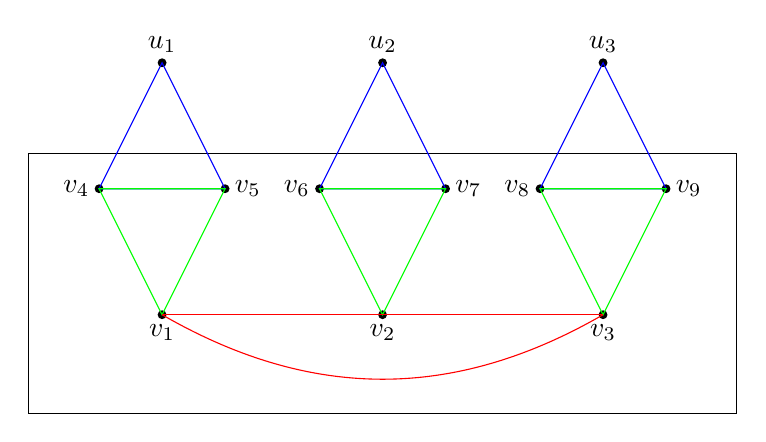
\begin{tikzpicture}[scale=0.8,
    node distance=1.5cm,
    set/.style={ellipse, draw, minimum width=1cm, minimum height=2cm},
    smallset/.style={ellipse, draw, minimum width=0.23cm, minimum height=0.9cm},
    label/.style={above, font=\normalsize},
    point/.style={circle, fill=black, inner sep=1pt},
    box/.style={draw, rectangle, minimum width=5.2cm, minimum height=3cm},
    verysmallset/.style={ellipse, draw, minimum size=0pt,  % 必须先取消默认限制
    inner sep=0pt,     % 取消内边距
    outer sep=0pt, minimum width=0.2cm, minimum height=0.5cm},
    box/.style={draw, rectangle, minimum width=9cm, minimum height=3.3cm},
]
\node[box, fill=blue!0] (A1) at (3.5,-0.5) {};
    \coordinate (a) at (0, 3);
    \fill (a) circle (2pt);  % 小圆圈，半径2pt
    
    \coordinate (b) at (-1, 1);
    \fill (b) circle (2pt);
    
    \coordinate (c) at (1, 1);
    \fill (c) circle (2pt);
    
    \coordinate (d) at (3.5, 3);
    \fill (d) circle (2pt);
    
    \coordinate (e) at (2.5, 1);
    \fill (e) circle (2pt);
    
    \coordinate (f) at (4.5, 1);
    \fill (f) circle (2pt);
    
    \coordinate (g) at (7, 3);
    \fill (g) circle (2pt);
    
    \coordinate (h) at (6, 1);
    \fill (h) circle (2pt);
    
    \coordinate (i) at (8, 1);
    \fill (i) circle (2pt);
    
    \coordinate (j) at (0, -1);
    \fill (j) circle (2pt);
    
    \coordinate (k) at (3.5, -1);
    \fill (k) circle (2pt);
    
    \coordinate (l) at (7, -1);
    \fill (l) circle (2pt);

    % 绘制蓝色三角形
    \draw[blue] (a) -- (b) -- (c) -- cycle;
    \draw[blue] (d) -- (e) -- (f) -- cycle;
    \draw[blue] (g) -- (h) -- (i) -- cycle;

    % 绘制绿色线段
    \draw[green] (b) -- (c) -- (j) -- cycle;
    \draw[green] (e) -- (f) -- (k) -- cycle;
    \draw[green] (h) -- (i) -- (l)--cycle;
    
    % 绘制红色曲线
    \draw[red] (j) -- (k);

    \draw[red] (k) -- (l);

    \draw[red]
    (j) to[out=-30, in=-150] (l);

    % 标注各点字母
    \node[above] at (a) {$u_1$};
    \node[left] at (b) {$v_4$};
    \node[right] at (c) {$v_5$};
    \node[above] at (d) {$u_2$};
    \node[left] at (e) {$v_6$};
    \node[right] at (f) {$v_7$};
    \node[above] at (g) {$u_3$};
    
    \node[left] at (h) {$v_8$};
    \node[right] at (i) {$v_9$};
    \node[below] at (j) {$v_1$};
    \node[below] at (k) {$v_2$};
    \node[below] at (l) {$v_3$};
\end{tikzpicture}
    \caption{A $K_3$-absorber for $\{u_1,u_2,u_3\}$.}
    \label{fig:absorber}
\end{figure}
\begin{lemma}[Absorbing lemma]\label{absorbing}
    Let $0<\frac{1}{n}\ll \eps\ll \alpha\ll \xi\ll \gamma\ll \frac{1}{r}$ and $r\ge 3$. Assume that $G$ is a graph on $n$ vertices such that $\sigma(G)\geq 2(1-\frac{1}{r}-\alpha)n$. If $G$ does not contain any $\gamma$-independent set of size $\frac{n}{r}$, then $G$ contains an  $\eps$-absorbing set $M$ of size at most $2\xi n$. %$|M|\leq 2\xi n$ and $M$ is a $K_r$-absorber for any $W\subset V(G)\setminus M$ with  $|W|\in r\mathbb{N}$ and $|W|\leq \eps n$. 
\end{lemma}
Using Lemmas \ref{almost-cover} and \ref{absorbing}, whose proofs are deferred to later subsections, we now prove Theorem~\ref{non-extremal}.
%The proofs of Lemmas \ref{almost-cover} and \ref{absorbing} will be given in the latter subsections. We now prove Theorem \ref{non-extremal} by Lemmas \ref{almost-cover} and \ref{absorbing}. 
\begin{proof}[\bf Proof of Theorem \ref{non-extremal}]
    Let $0<\frac{1}{n}\ll \mu\ll\eps\ll\alpha\ll \xi\ll \gamma\ll \frac{1}{r}$. Assume that $G$ is a graph on $n$ vertices and $\sigma(G)\geq 2(1-\frac{1}{r}-\alpha)n$. By Lemma \ref{absorbing}, $G$ contains an $\eps$-absorbing set $M$ such that $|M|\leq 2\xi n$. % and $M$ is a  $K_r$-absorber for any $W\subset V(G)\setminus M$ with  $|W|\in r\mathbb{N}$ and $|W|\leq \mu n$. 
    Let $G':=G-M$ and $n':=|G'|\geq (1-2\xi)n$. Therefore, 
    $$
    \sigma(G')\geq 2\Big(1-\frac{1}{r}-\alpha\Big)n-4\xi n\geq 2\Big(1-\frac{1}{r}-4\xi\Big)n'. 
    $$
    Applying Lemma \ref{almost-cover} on $G'$ yields that $G'$ has a $K_r$-tiling, say $\mathcal{K}$, that covers all but at most $\mu n'$ vertices. Denote by $U$ the set of vertices in $G'$ that are not covered by $\mathcal{K}$.  Together with the absorbing property of $M$, one has $G[M\cup U]$ contains a $K_r$-factor $\mathcal{K}'$. Hence, $\mathcal{K}\cup \mathcal{K}'$ is a $K_r$-factor of $G$, as desired. 
\end{proof}

\subsection{Regularity}
We begin by defining regularity for graphs.
\begin{definition}
  Given a graph $G$ and a pair $(X,Y)$ of vertex-disjoint subsets in $V(G)$, the \textit{density} of $(X,Y)$ is defined as 
  $$
  d(X,Y)=\frac{e(G[X,Y])}{|X||Y|}.
  $$
  Given a constant $\eps>0$, we say that $(X,Y)$ is an $\eps$-\textit{regular pair} in $G$ if for all $X'\subseteq X$, $Y'\subseteq Y$ with $|X'|\geq \eps |X|$ and $|Y'|\geq \eps |Y|$, we have 
        $$
          \left|d(X',Y')-d(X,Y)\right|\leq \eps.
        $$
Moreover, a pair $(X,Y)$ is called $(\eps,d)$-\textit{regular} for some $d>0$ if $(X,Y)$ is $\eps$-regular and $d(X,Y)\geq d$. 
\end{definition}

%The next observation establishes that every large subgraph of a regular pair is also regular. 
\begin{lemma}[Slicing lemma  \cite{Komlos2000}]\label{regular-subgraph}
    Let $0<\eps<\alpha$ and $\eps':=\max\{\eps/\alpha,2\eps\}.$ Let $(X,Y)$ be an $\eps$-regular pair of density $d$. Suppose $X'\subseteq X$ and $Y'\subseteq Y$ with $|X'|\geq \alpha |X|$ and $|Y'|\geq \alpha |Y|$. Then $(X',Y')$ is an $\eps'$-regular pair with density $d'$ where $|d'-d|<\eps$. 
\end{lemma} 

We next state the degree form of Szemer\'{e}di's Regularity Lemma, which can be easily derived from the classical version \cite{Szeme1978}.

\begin{lemma}[Degree form of the Regularity Lemma  \cite{ADLR1994,Szeme1978}]\label{thm: degree form of RL}
For every $\eps>0$, there exist integers $M$ and $n_0$ such that the following holds for any $d\in [0,1]$ and any positive integer $n\ge n_0$. Let $G$ be a graph on $n$ vertices. Then we can find in time $O(n^{2.376})$ a partition $\mathcal{P}:=\{V_0,V_1, \dots,V_k\}$ of $V(G)$ and a spanning subgraph $G'\subseteq G$ with the following properties:
\begin{enumerate}[label = (\arabic{enumi})]
\rm \item\label{pro1} $\frac{1}{\eps}\le k \le M$;
\rm \item\label{pro2} $|V_0|\le \eps n$ and $|V_1|=|V_2|=\dots=|V_k|=:m$; % with $m\le \eps n$;
\rm \item\label{pro3} $d_{G'}(v)>d_{G}(v)-(d+2\eps)n$ for every $v\in V(G)$;
\rm \item\label{pro4} $e(G'[V_i])=0$ for each $i\in [k]$;
\rm \item\label{pro5} for $1\le i<j\le k$, each pair $(V_i,V_j)$ is $\eps$-regular in $G'$ with density {either} $0$ or at least $d$.
\end{enumerate}
\end{lemma}

The sets $V_i$ are called \textit{clusters} and  $V_0$ is the \textit{exceptional set}. 
A widely used auxiliary graph associated with the regular partition is the \textit{reduced graph} defined as follows. %An \textit{weighted  reduced graph} of $G$ is a union of $G_{\ell}$ that is defined on the vertex set $\{V_1,\dots, V_k\}$ for each color $\ell\in [p]$ and we employ the following definitions.
%by assigning the density between each pair of partitions as weights under the color $\ell\in [p]$ 
\begin{definition}[Reduced graph]
Let $G$ be an $n$-vertex graph. Given parameters $\eps>0$ and $d\in [0,1]$, let $G'$ be a spanning subgraph of $G$ and $\mathcal{P}=\{V_0,V_1, \dots,V_k\}$ be a partition of $V(G)$, as given in Lemma \ref{thm: degree form of RL}. We define the \textit{reduced graph} $R:=R(\eps,d)$ for $\mathcal{P}$ as follows: %Apply Lemma \ref{thm: degree form of RL} to $G$, with parameters $\eps,{\bf d}$ to obtain a spanning subgraph $G'$ and a partition $\mathcal{P}=\{V_0,V_1, \dots,V_k\}$ of $V(G)$. Then 
$R$ is a graph on vertex set $\{V_1,\ldots,V_k\}$ in which $V_i$ and $V_j$ are adjacent if and only if $(V_i,V_j)$ has density at least $d$ in $G'$.
\end{definition}

%Given a real number $d\in [0,1]$, the $d$-{\textit{reduced graph}} $R_d$ of $\mathcal{P}$ is a graph defined on the vertex set $\{V_1,\ldots,V_k\}$, such that ${ij}\in E(R_d)$ if and only if $(V_i,V_j)$ has density at least $d$ in $G'$.

The next lemma states that clusters inherit the Ore-type condition in the reduced graph.
\begin{lemma}[\cite{Kuhn}]\label{reduced graph}
    Given a constant $c$, let $G$ be a graph on $n$ vertices such that $\sigma(G)\geq cn$. Suppose we have applied Lemma \ref{thm: degree form of RL} with parameters $\eps$ and $d$
 to $G$. Let $R$ be the corresponding reduced graph. Then $\sigma(R)\geq (c-2d-4\eps)|R|$.
\end{lemma}



The following result will be used to convert an almost perfect $K_r$-tiling in a reduced graph into an almost perfect $K_r$-tiling in the original graph $G$.
\begin{lemma}[\cite{Alon1992}]\label{reduce-original}
    Let $\eps,d>0$ and $m,r\in \mathbb{N}$ such that $0<{1}/{m}\ll \eps\ll d\ll 1/r$. Let $H$ be a graph obtained from $K_r$ by replacing every vertex with $m$ independent  vertices and every edge with an $\eps^2$-regular pair of density at least $d$. Then $H$ admits a $K_r$-tiling that covers all but at most $\eps m r$ vertices.
\end{lemma}
Our next lemma shows that the reduced graph inherits the property of having no large almost independent set. 
\begin{lemma}\label{blow-up}
    Let $r,n,t\in \mathbb{N}$ with  $0<1/n\ll \eps\ll d\ll\gamma\ll 1/r$, and % Given a constant $c$, 
    let $G$ be an $n$-vertex graph containing no  $\gamma$-independent set of size ${n}/{r}$. % on $n$ vertices such that $\sigma(G)\geq cn$. 
    Suppose we have applied Lemma \ref{thm: degree form of RL} with parameters $\eps$ and $d$ 
 to $G$, yielding a reduced graph $R$ for a partition $\mathcal{P}$ of $V(G)$. %If $G$ contains no  $\gamma$-independent set of size $\frac{n}{r}$, t
 Then,  $R[t]$ can be viewed as a subgraph of some reduced graph $R':=R(2\eps t,d/2)$ for a refinement partition of $\mathcal{P}$. Moreover, $R[t]$ contains no  ${\gamma}/2$-independent set of size ${tk}/{r}$. 
\end{lemma}
\begin{proof}
Let $\mathcal{P}:=\{V_0,V_1, \dots,V_k\}$ be a partition of  $V(G)$ obtained in Lemma \ref{thm: degree form of RL}. For each $i\in [k]$, partition $V_i$ into $V_{i,0}\cup V_{i,1}\cup \cdots\cup V_{i,t}$, where $m':=|V_{i,j}|=\lfloor\frac{m}{t}\rfloor\geq \frac{m}{2t}$ for each $1\leq j\leq t$. Since $mk\geq (1-\eps)n$, one has
$$
m'\cdot |R[t]|=\lfloor\frac{m}{t}\rfloor\cdot kt\geq mk-kt\geq (1-2\eps)n.
$$
Lemma \ref{regular-subgraph} implies that if $(V_{i_1},V_{i_2})_{G'}$ is $\eps$-regular with density at least $d$, then $(V_{i_1,j_1},V_{i_2,j_2})_{G'}$ is $2\eps t$-regular with density at least $d-\eps\geq d/2$ for all $1\leq j_1,j_2\leq t$. In particular, we can label the vertex set of $R[t]$ so that $V(R[t])=\{V_{i,j}:1\leq i\leq k,1\leq j\leq t\}$, where $V_{i_1,j_1}V_{i_2,j_2}\in E(R[t])$ implies that $(V_{i_1,j_1},V_{i_2,j_2})_{G'}$ is $2\eps t$-regular with density at least $d-\eps\geq d/2$. That is, $R[t]$ can be viewed as a subgraph of some reduced graph $R':=R(2\eps t,d/2)$ for the partition $\big\{(\bigcup_{i\in [k]}V_{i,0}\cup V_0), V_{1,1}, \ldots,  V_{1,t},\ldots, V_{k,1}, \ldots,  V_{k,t}\big\}$.%$R[t]$ can be viewed as the reduced graph of $G$ by applying Lemma \ref{thm: degree form of RL} with parameters $2\eps t$ and $d/2$. 

    Next, we prove that $R[t]$ contains no ${\gamma}/2$-independent set of size $t{k}/{r}$.  Suppose that %$R$ contains a ${\gamma}$-independent set of size $\frac{k}{r}$. That is, 
    there exists a set $S:=\{V_{i_1,j_1},\ldots,V_{i_{{tk}/{r}},j_{{tk}/{r}}}\}\subseteq V(R[t])$ such that $|E((R[t])[S])|\leq \frac{\gamma}{2} (tk)^2$. Therefore, 
    $$
    |V_{i_1,j_1}\cup \cdots\cup V_{i_{{tk}/{r}},j_{{tk}/{r}}}|\geq \frac{(1-2\eps)n}{r}\ \text{and}\ |E(G[V_{i_1,j_1}\cup \cdots\cup V_{i_{{tk}/{r}},j_{{tk}/{r}}}])|\leq \frac{{\gamma}}{2} (tk)^2m'^2\leq \frac{{\gamma}}{2} n^2. 
    $$
     By augmenting $V_{i_1,j_1}\cup \cdots\cup V_{i_{{tk}/{r}},j_{{tk}/{r}}}$ with at most $2\eps n/r$ additional vertices, we obtain a $\gamma$-independent set in $G$ of size at least $\frac{n}{r}$, 
    a contradiction. 
    %Therefore, $R[t]$ also contains no  ${\gamma}/2$-independent set of size ${tk}/{r}$.
\end{proof}
%The \textit{maximum $(K_r,K_{r-1},\ldots,K_1)$-factor} of $G$ is a collection of vertex-disjoint subgraphs of $G$ with the vertex set $V_r,\ldots,V_1$ which is union of $V(K_i)$ respectively covering all the vertices of $V(G)$ such that the number of $K_s$ copies is maximum in $G[V(G)\setminus (\overset{r}{\underset{i=r-s+1}\cup}V_i)]$.
\subsection{Proof of Lemma \ref{almost-cover}}\label{section4.2}

We first prove the almost cover lemma. 

\begin{definition}\label{maximum-factor}
    A \textit{maximum $(K_r,K_{r-1},\ldots,K_1)$-factor} of a graph $G$ is a collection of vertex-disjoint subgraphs ${H_1, \ldots, H_k}$ of $G$ such that
\begin{itemize}
    \item each $H_i$ is isomorphic to some $K_s$ where $1 \leq s \leq r$; 
    \item the vertex sets of these subgraphs form a partition $V(G) = U_r \cup U_{r-1} \cup \cdots \cup U_1$, where $U_s$ consists of the vertices covered by $K_s$ components;
    \item for each $s\in \{r,r-1,\ldots,1\}$, the number of $K_s$ copies in $G\left[V(G) \setminus \left( \bigcup_{i=s+1}^r U_i \right) \right]$ is maximized.
\end{itemize}
\end{definition}

\begin{proof}[\bf Proof of Lemma \ref{almost-cover}]
   Given parameters satisfying 
   $$0<\frac{1}{n}\ll \eps\ll d\ll\mu\ll \alpha\ll \gamma\ll \frac{1}{r},
   $$
   assume that $G$ is an $n$-vertex graph with $\sigma(G)\geq 2(1-{1}/{r}-\alpha)n$ and $G$ contains no  $\gamma$-independent set of size $n/r$. By applying Lemma \ref{thm: degree form of RL} on $G$ with parameters $\eps$ and $d$, we obtain  a partition $\mathcal{P}:=\{V_0,V_1,\ldots,V_k\}$ with $k \geq \frac{1}{\eps}$ and a spanning subgraph $G'\subseteq G$ with properties $(1)$-$(5)$ as stated. Let $R$ be the reduced graph corresponding to $\mathcal{P}$. Based on Lemma \ref{reduced graph}, we have $\sigma(R)\geq 2(1-\frac{1}{r}-2\alpha)k$. Define $S:=\{v\in V(R):d_R(v)<(1-\frac{1}{r}-2\alpha)k\}$.

   
   
   
   Choose a maximum $(K_r,K_{r-1},\ldots,K_1)$-factor of $R$ and assume $V(R) = U_r \cup U_{r-1} \cup \cdots \cup U_1$, where $U_s$ consists of the vertices covered by $K_s$ components for each $s\in [r]$. Hence $|(V(G)\setminus U_r)\cap S|\leq r-1$. Therefore, there are at most $r-1$ components $K_t$ with $t<r$ that intersect with $S$. In the following, if $K_t$ is a clique in the maximum $(K_r,K_{r-1},\ldots,K_1)$-factor of $R$, then we simply say $K_t\in U_t$ for each $t\in [r]$.  %For each $i\in [r]$, define $R_s:=R\left[V(R) \setminus \left( \bigcup_{i=s+1}^r U_i \right) \right]$. %There are at least $(1-r^2\eps)n$ vertices covered by vertex-disjoint $K_r$. %Choose a maximum $K_r$-tiling of $G$, denote $V_r$ the set of vertices in such a $K_r$-tiling and let $G_r:=G-V_r$. Clearly, $|V(G_r)\cap S|\leq r-1$. We can define $G_i,V_i$ repeatedly for each $i\in \{r-1,\ldots,2\}$ and 
    %Notice that $|V(G_{s})\cap S|\leq s$ for each $i\in [r-1]$. 
\begin{claim}\label{a-almost}
    $|U_r|\geq (1-\alpha r^2)k.$
\end{claim}
\begin{proof}[Proof of Claim \ref{a-almost}]
    Choose a minimum constant $\zeta$ satisfying $\zeta\geq r\alpha$ and $r|(1+\zeta)k$, let $R^*:=R\vee K_{\zeta k}$ and $k^*:=|V(R^*)|=(1+\zeta)k$. Notice that if $xy\notin E(R^*)$, then $xy\notin E(R)$. Hence, for each edge $xy\notin E(R^*)$, we have  
    $$
    d_{R^*}(x)+d_{R^*}(y)=d_{R}(x)+d_{R}(y)+2\zeta k\geq 2\Big(1-\frac{1}{r}-\alpha+\zeta\Big)k\geq 2\Big(1-\frac{1}{r}\Big)k^*,
    $$
    where the last inequality holds as $\zeta \geq r\alpha$ and $r\ge 3$. 
    Together with Theorem \ref{KK2008}, we obtain that $R^*$ contains a $K_r$-factor. It follows from $\zeta k\leq r\alpha k+r$ that $|U_r|\geq (1-\alpha  r^2)k$, as desired. 
\end{proof}
In the following claim, we consider $K_r$-tilings in the blow-up graph of $R$. % We first give the following claim.
\begin{claim}\label{reduced-blow}
    There exists an integer $z$ such that the blow-up graph $R[2^{z(r-1)}]$, has a $K_r$-tiling covering at least $(1-\mu/2)|R[2^{z(r-1)}]|$ vertices.
\end{claim}
\begin{proof}[Proof of Claim \ref{reduced-blow}]
%Based on the $(K_r, K_{r-1}, \ldots, K_1)$-factor of $R$ described above, w
If $|V(R)\setminus U_r|\leq \frac{\mu}{2}k$, then  we are done. So, we assume that $|U_r|:=q$ with $(1-\alpha r^2)k\leq q\leq (1-\mu/2)k$. Then there are at least $\frac{\mu}{2}k-(r-1)^2$ vertices that are  in $K_t\in U_t$ with $t<r$ and $V(K_t)\cap S=\emptyset$. 

We construct an auxiliary bipartite graph $H=(A,B)$, where each $K_r\in U_r$ corresponds to a vertex $v_{K_r}$ in $A$ and each $K_t\in U_t$ with $t<r$ and $V(K_t)\cap S=\emptyset$ corresponds to a vertex $v_{K_t}$ in $B$; $v_{K_r}v_{K_t}\in E(H)$ if and only if $|N_R(K_t)\cap V(K_r)|\geq r-t+1$. Choose a maximum matching $M$ in $H$. Hence, for each $v_{K_t}\in B\setminus V(M)$, we have $|N_R(K_t)\cap V(K_r)|\leq r-t$ for each $v_{K_r}\in A\setminus V(M)$. Furthermore, Claim~\ref{a-almost} implies that $|E(M)|\leq \alpha r^2 k$. Next, we will show that each $K_t\in U_t$ with $t<r$  and $V(K_t)\cap S=\emptyset$ can be augmented to a copy of $K_{t+1}$ in the blow-up graph $R[2]$.  

\begin{fact}\label{claim-b1}
    If $v_{K_r}v_{K_t}\in E(M)$, then $(K_r\cup K_t)[2]$ contains $2K_r\cup K_{t+1}\cup K_{t-1}$ as a subgraph. 
\end{fact}
\begin{proof}[Proof of Fact  \ref{claim-b1}]
  Notice that $|N_R(K_t)\cap V(K_r)|\geq r-t+1$.  Let $V(K_r)=\{u_1,\ldots,u_r\}$, $V(K_t)=\{w_1,\ldots,w_t\}$,  and assume $\{u_1,\ldots,u_{r-t+1}\}\subseteq N_R(K_t)\cap V(K_r)$. Consider the blow-up graph $(K_r \cup K_t)[2]$ with vertex set $\{u^1,u^2:u\in V(K_r\cup K_t)\}$. It is straightforward to verify that $(K_r \cup K_t)[2]$ contains four disjoint subgraphs induced by the following vertex sets: $\{u_1^1,\ldots,u_r^1\}$, $\{u_1^2,\ldots,u_{r-t}^2,w_1^1,\ldots,w_t^1\}$, $\{w_1^2,\ldots,w_t^2,u_{r-t+1}^2\}$, and $\{u_{r-t+2}^2,\ldots, u_r^2\}$. That is, $(K_r\cup K_t)[2]$ contains $2K_r\cup K_{t+1}\cup K_{t-1}$ as a subgraph. (see Figure \ref{fig:almost-1} for $r=3$ and $t=2$). 
\end{proof}
%It is straightforward to check that if $v_{K_r}v_{K_t}\in E(M)$, then $(K_r\cup K_t)[2]$ contains $2K_r\cup K_{t+1}\cup K_{t-1}$ as a subgraph (see Figure \ref{fig:almost-1} for $r=3$ and $t=2$).
 %Let $t$ be an integer such that $|U_t|=\max\{|U_i|:i\in [r-1]\}$. Notice that 
%$$
%\frac{|U_t|}{t}\geq \frac{\mu k}{t(r-1)}>t\ \text{and}\ |U_t\cap S|\leq t.
%$$
%Hence $R_t$ contains a copy of $K_t$, say $K$, such that $V(K)\cap S=\emptyset$. %hoose such a $K_t$ in $U_t$. 

%Notice that if there are $K_r\in U_r$ and $K_t\in U_t$ with $t<r$ such that $|N_R(K_t)\cap V(K_r)|\geq r-t+1$, then $(K_r\cup K_t)[2]$ contains $2K_r\cup K_{t+1}\cup K_{t-1}$ as a subgraph (see Figure \ref{fig:almost-1} for $r=3$ and $t=2$).  %corresponding to the blow up set of $V(K_r)\cup V(K_t)$. 
%That is to say, 
%$$
%\frac{|V(R_{t})|}{|V(R)|}-\frac{|V(R[2]_{t})|}{|V(R[2])|}=\frac{t+1}{2k}.
%$$

\begin{figure}[ht!]
    \centering
    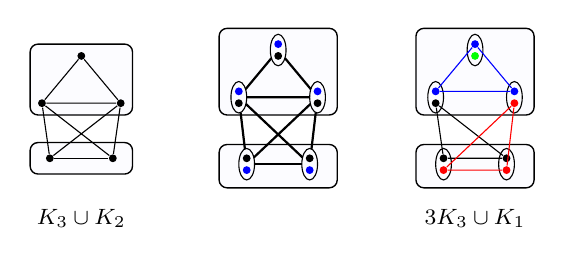
\begin{tikzpicture}[
bigroundbox/.style={
        draw, 
        rectangle, 
        minimum width=1.3cm, 
        minimum height=0.9cm,
        rounded corners=1mm,  % 控制圆角大小
        line width=0.5pt,       % 边框粗细
        fill=blue!1          % 填充色
    },
   roundbox/.style={
        draw, 
        rectangle, 
        minimum width=1.3cm, 
        minimum height=0.4cm,
        rounded corners=1mm,  % 控制圆角大小
        line width=0.5pt,       % 边框粗细
        fill=blue!1          % 填充色
    },
    bbigroundbox/.style={
        draw, 
        rectangle, 
        minimum width=1.5cm, 
        minimum height=1.1cm,
        rounded corners=1mm,  % 控制圆角大小
        line width=0.5pt,       % 边框粗细
        fill=blue!1          % 填充色
    },
    bbbigroundbox/.style={
        draw, 
        rectangle, 
        minimum width=1.5cm, 
        minimum height=0.55cm,
        rounded corners=1mm,  % 控制圆角大小
        line width=0.5pt,       % 边框粗细
        fill=blue!1          % 填充色
    },
    point/.style={circle, fill=black, inner sep=1pt},
    set/.style={ellipse, draw, minimum size=0pt,  % 必须先取消默认限制
    inner sep=0pt,     % 取消内边距
    outer sep=0pt, minimum width=0.2cm, minimum height=0.4cm},
    label/.style={above, font=\footnotesize},
]
\node[bigroundbox] (box) at (0.5,0.3) {};
\node[roundbox] (box2) at (0.5,-0.7) {};

\node[point] (A1) at (0,0) {};
\node[point] (A2) at (1,0) {};
\node[point] (A3) at (0.5,0.6) {};
\draw (A1)--(A2)--(A3)--(A1);

\node[point] (B1) at (0.1,-0.7) {};
\node[point] (B2) at (0.9,-0.7) {};

\draw (B1)--(B2);

\draw (A1)--(B1)--(A2)--(B2)--(A1);
\node[label] at (0.5,-1.7) {{{$K_3\cup K_2$}}};
\node[bbigroundbox] (box) at (3,0.4) {};
\node[bbbigroundbox] (box2) at (3,-0.8) {};

\node[point] (A1) at (2.5,0) {};
\node[set] (cycle1) at (2.5,0.075) {};
\node[point,blue] (A01) at (2.5,0.15) {};
\node[point] (A2) at (3.5,0) {};
\node[set] (cycle2) at (3.5,0.075) {};
\node[point,blue] (A02) at (3.5,0.15) {};
\node[point] (A3) at (3,0.6) {};
\node[set] (cycle3) at (3,0.675) {};
\node[point,blue] (A03) at (3,0.75) {};
\draw[thick] (cycle1)--(cycle2)--(cycle3)--(cycle1);

\node[point] (B1) at (2.6,-0.7) {};
\node[set] (cycle4) at (2.6,-0.775) {};
\node[point,blue] (B01) at (2.6,-0.85) {};
\node[point] (B2) at (3.4,-0.7) {};
\node[set] (cycle5) at (3.4,-0.775) {};
\node[point,blue] (B02) at (3.4,-0.85) {};

\draw[thick] (cycle4)--(cycle5);

\draw[thick] (cycle1)--(cycle4)--(cycle2)--(cycle5)--(cycle1);

\node[bbigroundbox] (box) at (5.5,0.4) {};
\node[bbbigroundbox] (box2) at (5.5,-0.8) {};

\node[point] (A1) at (5,0) {};
\node[set] (cycle1) at (5,0.075) {};
\node[point,blue] (A01) at (5,0.15) {};
\node[point,red] (A2) at (6,0) {};
\node[set] (cycle2) at (6,0.075) {};
\node[point,blue] (A02) at (6,0.15) {};
\node[point,green] (A3) at (5.5,0.6) {};
\node[set] (cycle3) at (5.5,0.675) {};
\node[point,blue] (A03) at (5.5,0.75) {};

\node[point] (B1) at (5.1,-0.7) {};
\node[set] (cycle4) at (5.1,-0.775) {};
\node[point,red] (B01) at (5.1,-0.85) {};
\node[point] (B2) at (5.9,-0.7) {};
\node[set] (cycle5) at (5.9,-0.775) {};
\node[point,red] (B02) at (5.9,-0.85) {};
\draw[blue] (A01)--(A02)--(A03)--(A01);

\draw (A1)--(B1)--(B2)--(A1);
\draw[red] (A2)--(B01)--(B02)--(A2);
%\draw[thick] (cycle4)--(cycle5);

%\draw[thick] (cycle1)--(cycle4)--(cycle2)--(cycle5)--(cycle1);
\node[label] at (5.5,-1.7) {{{$3K_3\cup K_1$}}};
\end{tikzpicture}
    \caption{$|N_R(K_t)\cap V(K_r)|\geq r-t+1$ for $r=3$ and $t=2$.}
    \label{fig:almost-1}
\end{figure}

%one may use $K_i$ with $i\geq s+1$ to cover more vertices in  


Choose a clique $K_t\in U_t$ with $v_{K_t}\in B\setminus V(M)$, say $K$. % Next, we assume that each $K_r$ satisfying $|N_R(K)\cap V(K_r)|\leq r-t$. 
Denote 
\begin{align*}
   &X:=\{v_{K_r}\in  A\setminus V(M): |N_R(K)\cap V(K_r)|=r-t\}\ \text{and}\ Y:=A\setminus (V(M)\cup X),%\\
   %&Y=\{v_{K_r}\subseteq A\setminus V(M): |N_R(K)\cap V(K_r)|<r-t\}, 
\end{align*}
assume $x:=|X|$ and $y:=|Y|$. It follows from Claim \ref{a-almost} that  $x+y\geq (\frac{1}{r}-\alpha r-\alpha r^2)k$. Moreover, 
$$
tx+(t+1)y\leq |V(R)\setminus N_R(K)|=k-|N_R(K)|\leq  t\Big(\frac{1}{r}+2\alpha\Big)k,
$$
the last inequality follows by $V(K)\cap S=\emptyset$. 
Therefore, $y\leq t(2\alpha+\alpha r+\alpha r^2)k$ and $x\geq (\frac{1}{r}-2\alpha r^3)k$. 


If $|N_R(w)\cap V(K_r)|=r$ for some $w\in V(K)$ and $v_{K_r}\in X$, then a similar proof to Fact~\ref{claim-b1} shows that $(K_r\cup K)[2]$ contains $2K_r\cup K_{t+1}\cup K_{t-1}$ as a subgraph. Now, we assume that $|N_R(w)\cap V(K_r)|\leq r-1$ for each $w\in V(K)$ and $v_{K_r}\in X$. %  $R[2]$ contains $2K_r\cup K_{t+1}\cup K_{t-1}$. 
Choose $w\in V(K)$, denote 
\begin{align*}
&X^w:=\{v_{K_r}\in  A\setminus V(M): |N_R(w)\cap V(K_r)|=r-1\}\ \text{and}\\
&Y^w:=\{v_{K_r}\in  A\setminus V(M): |N_R(w)\cap V(K_r)|<r-1\},
\end{align*}
assume $x^w:=|X^w|$ and $y^w:=|Y^w|$.  Similarly, we have 
$$
x^w+y^w\geq \Big(\frac{1}{r}-\alpha r-\alpha r^2\Big)k\ \text{and}\ x^w+2y^w\leq \Big(\frac{1}{r}+2\alpha\Big)k.
$$
Hence $y^w\leq (2\alpha+2\alpha r+2\alpha r^2)k$ and $x^w\geq (\frac{1}{r}-4\alpha r^2)k$. Note that $X\cup (\bigcup_{u\in V(K)}X^u)\subseteq A\setminus V(M)$ and $|A|\leq \frac{|U_r|}{r}<\frac{k}{r}$. Thus,  $$\ell:=\Big|X\cap (\bigcap_{u\in V(K)}X^u)\Big|\geq \Big(\frac{1}{r}-7\alpha r^3\Big)k.$$  

For each $i\in [\ell]$, choose a vertex $w_i$ from each copy of  $K_r$, say $K^i$, with $v_{K^i}\in X\cap (\bigcap_{u\in V(K)}X^u)$ such that $w_iw\notin E(R)$. % is not adjacent to $w_i$ for each $i$. 
It follows from Lemma \ref{blow-up} that $R$ contains no $\gamma/2$-independent set of size ${k}/{r}$. Thus, there is an edge, say $w_1w_2$, in $R[\{w_1,\ldots,w_{\ell}\}]$. We claim that $w_1,w_2$ are adjacent to all vertices in $V(K)\setminus \{w\}$. Otherwise, suppose that $w_1w'\notin E(R)$ for some $w'\in V(K)\setminus \{w\}$. By the choice of $X\cap (\bigcap_{u\in V(K)}X^u)$, we know that at most $t$ edges are missing between $V(K)$ and $V(K^1)$ in $R$. However, at least two vertices in $V(K)$ are not adjacent to the vertex $w_1$. Hence,  at most $t-1$ vertices in $K^1$ has non-neighbors in $K$. It follows that $|N_R(K)\cap V(K^1)|\geq r-t+1$, a contradiction. Therefore, $(K^1\cup K^2\cup K)[2]$ contains $4K_r\cup K_{t+1}\cup K_{t-1}$, as shown by an argument similar to Fact~\ref{claim-b1}  (see Figure \ref{fig:almost-2} for $r=3$ and $t=2$). 
%Moreover, by Claim \ref{a-almost}, similar result holds for each $K_t\in Y\setminus V(M)$. 
\begin{figure}[ht!]
    \centering
    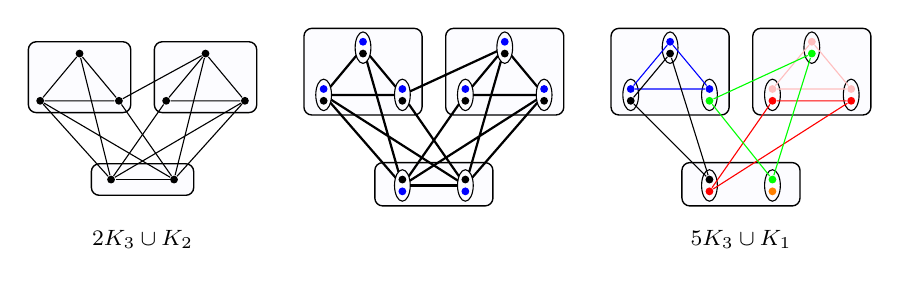
\begin{tikzpicture}[
bigroundbox/.style={
        draw, 
        rectangle, 
        minimum width=1.3cm, 
        minimum height=0.9cm,
        rounded corners=1mm,  % 控制圆角大小
        line width=0.5pt,       % 边框粗细
        fill=blue!1          % 填充色
    },
   roundbox/.style={
        draw, 
        rectangle, 
        minimum width=1.3cm, 
        minimum height=0.4cm,
        rounded corners=1mm,  % 控制圆角大小
        line width=0.5pt,       % 边框粗细
        fill=blue!1          % 填充色
    },
    bbigroundbox/.style={
        draw, 
        rectangle, 
        minimum width=1.5cm, 
        minimum height=1.1cm,
        rounded corners=1mm,  % 控制圆角大小
        line width=0.5pt,       % 边框粗细
        fill=blue!1          % 填充色
    },
    bbbigroundbox/.style={
        draw, 
        rectangle, 
        minimum width=1.5cm, 
        minimum height=0.55cm,
        rounded corners=1mm,  % 控制圆角大小
        line width=0.5pt,       % 边框粗细
        fill=blue!1          % 填充色
    },
    point/.style={circle, fill=black, inner sep=1pt},
    set/.style={ellipse, draw, minimum size=0pt,  % 必须先取消默认限制
    inner sep=0pt,     % 取消内边距
    outer sep=0pt, minimum width=0.2cm, minimum height=0.4cm},
    label/.style={above, font=\footnotesize},
]
\node[bigroundbox] (box) at (-0.3,0.3) {};
\node[bigroundbox] (box1) at (1.3,0.3) {};
\node[roundbox] (box2) at (0.5,-1) {};

\node[point] (A1) at (-0.8,0) {};
\node[point] (A2) at (0.2,0) {};
\node[point] (A3) at (-0.3,0.6) {};
\draw (A1)--(A2)--(A3)--(A1);

\node[point] (0A1) at (0.8,0) {};
\node[point] (0A2) at (1.8,0) {};
\node[point] (0A3) at (1.3,0.6) {};
\draw (0A1)--(0A2)--(0A3)--(0A1);
\draw (A2)--(0A3);
\node[point] (B1) at (0.1,-1) {};
\node[point] (B2) at (0.9,-1) {};

\draw (B1)--(B2);

\draw (A3)--(B1)--(A1)--(B2)--(A2);
\draw (0A1)--(B1)--(0A2)--(B2)--(0A3);
\node[label] at (0.5,-2) {{{$2K_3\cup K_2$}}};
\node[bbigroundbox] (box) at (3.3,0.37) {};
\node[bbigroundbox] (box2) at (5.1,0.37) {};
\node[bbbigroundbox] (box3) at (4.2,-1.06) {};

\node[point] (A1) at (2.8,0) {};
\node[set] (cycle1) at (2.8,0.075) {};
\node[point,blue] (A01) at (2.8,0.15) {};
\node[point] (A2) at (3.8,0) {};
\node[set] (cycle2) at (3.8,0.075) {};
\node[point,blue] (A02) at (3.8,0.15) {};
\node[point] (A3) at (3.3,0.6) {};
\node[set] (cycle3) at (3.3,0.675) {};
\node[point,blue] (A03) at (3.3,0.75) {};
\draw[thick] (cycle1)--(cycle2)--(cycle3)--(cycle1);

\node[point] (0A1) at (4.6,0) {};
\node[set] (cycle01) at (4.6,0.075) {};
\node[point,blue] (0A01) at (4.6,0.15) {};
\node[point] (0A2) at (5.6,0) {};
\node[set] (cycle02) at (5.6,0.075) {};
\node[point,blue] (0A02) at (5.6,0.15) {};
\node[point] (0A3) at (5.1,0.6) {};
\node[set] (cycle03) at (5.1,0.675) {};
\node[point,blue] (0A03) at (5.1,0.75) {};
\draw[thick] (cycle01)--(cycle02)--(cycle03)--(cycle01);
\draw[thick] (cycle2)--(cycle03);

\node[point] (B1) at (3.8,-1) {};
\node[set] (cycle4) at (3.8,-1.075) {};
\node[point,blue] (B01) at (3.8,-1.15) {};
\node[point] (B2) at (4.6,-1) {};
\node[set] (cycle5) at (4.6,-1.075) {};
\node[point,blue] (B02) at (4.6,-1.15) {};

\draw[thick] (cycle4)--(cycle5);

\draw[thick] (cycle3)--(cycle4)--(cycle1)--(cycle5)--(cycle2);
\draw[thick] (cycle01)--(cycle4)--(cycle02)--(cycle5)--(cycle03);

\node[bbigroundbox] (box) at (7.2,0.37) {};
\node[bbigroundbox] (box2) at (9,0.37) {};
\node[bbbigroundbox] (box3) at (8.1,-1.06) {};

\node[point] (A1) at (6.7,0) {};
\node[set] (cycle1) at (6.7,0.075) {};
\node[point,blue] (A01) at (6.7,0.15) {};
\node[point,green] (A2) at (7.7,0) {};
\node[set] (cycle2) at (7.7,0.075) {};
\node[point,blue] (A02) at (7.7,0.15) {};
\node[point] (A3) at (7.2,0.6) {};
\node[set] (cycle3) at (7.2,0.675) {};
\node[point,blue] (A03) at (7.2,0.75) {};

\node[point,red] (0A1) at (8.5,0) {};
\node[set] (cycle01) at (8.5,0.075) {};
\node[point,pink] (0A01) at (8.5,0.15) {};
\node[point,red] (0A2) at (9.5,0) {};
\node[set] (cycle02) at (9.5,0.075) {};
\node[point,pink] (0A02) at (9.5,0.15) {};
\node[point,green] (0A3) at (9,0.6) {};
\node[set] (cycle03) at (9,0.675) {};
\node[point,pink] (0A03) at (9,0.75) {};

\node[point] (B1) at (7.7,-1) {};
\node[set] (cycle4) at (7.7,-1.075) {};
\node[point,red] (B01) at (7.7,-1.15) {};
\node[point,green] (B2) at (8.5,-1) {};
\node[set] (cycle5) at (8.5,-1.075) {};
\node[point,orange] (B02) at (8.5,-1.15) {};
\draw[blue] (A01)--(A02)--(A03)--(A01);
\draw[pink] (0A01)--(0A02)--(0A03)--(0A01);



\draw (A1)--(B1)--(A3)--(A1);
\draw[red] (0A2)--(B01)--(0A1)--(0A2);
\draw[green] (A2)--(B2)--(0A3)--(A2);
%\draw[thick] (cycle4)--(cycle5);

%\draw[thick] (cycle1)--(cycle4)--(cycle2)--(cycle5)--(cycle1);
\node[label] at (8.1,-2) {{{$5K_3\cup K_1$}}};
\end{tikzpicture}
    \caption{$|N_R(K_t)\cap V(K_r)|\leq r-t$ for $r=3$ and $t=2$.}
    \label{fig:almost-2}
\end{figure}




By the above discussion, for each $K_t\in U_t$ with $t<r$ and $V(K_t)\cap S=\emptyset$, we conclude that 
\begin{itemize}
    \item either there exists a copy of $K_r\in U_r$ such that $(K_r\cup K_t)[2]$ contains $2K_r\cup K_{t+1}\cup K_{t-1}$,
    \item or there are two copies of $K_r\in U_r$ such that $(2K_r\cup K_t)[2]$ contains $4K_r\cup K_{t+1}\cup K_{t-1}$.
\end{itemize}
Moreover, we can choose the $K_r$ copies for different $K_t$ so that they are pairwise disjoint. Let $q$ be the number of vertices covered by $U_r$. Assume $|U_j|=\max\{|U_i|:i\in[r-1]\}$. Then $|U_j|\geq \frac{k-q}{2(r-1)}$. By applying the augmentation process to the cliques in $U_j$, we obtain a maximum $(K_r,K_{r-1},\ldots,K_1)$-factor of $R[2]$ such that copies of $K_i$ cover at least $2|U_i|$ vertices for all $i\in [r]\setminus \{j,j+1\}$, and copies of $K_{j+1}$ cover at least $2|U_{j+1}| + |U_j|$ vertices. (Here,  $2|U_{j+1}|$ and $|U_j|$  come from the original cliques in $U_{j+1}$  and the augmentation of cliques in $U_j$, respectively). %where $2|U_{j+1}|$ comes from  the original cliques in $U_{j+1}$ and $|U_j|$ comes from the augment of  cliques in $U_j$. 
By iterating this augmentation--first on the new $K_{j+1}$ copies, then on the resulting $K_{j+2}$ copies, and so forth, up to the $K_{r-1}$ copies, we ultimately construct a $K_r$-tiling within $R[2^{r-j}]$ of order at least 
 %Next, we do the  augmentation process for the new parts consisting of $K_{j+1}$ copies. 
%Repeat the above process, in $R[2^{r-j}]$, one may find a $K_r$-tiling of order at least 
$$
2^{r-j}|U_r|+2^{r-j-1}|U_{r-1}|+\cdots+|U_j|\geq 2^{r-j}q+|U_j|.
$$
Therefore, there exists a $K_r$-tiling in $R[2^{r-1}]$ covering at least 
$$
2^{r-1}q+\frac{|U_j|}{2^{r-1}}\cdot 2^{r-1}\geq q2^{r-1}+\frac{\mu k}{4(r-1)2^{r-1}}\cdot 2^{r-1}
$$
vertices, as $k-q\ge \mu k/2$. Thus, an additional  $\eta$-proportion of the vertices in $R[2^{r-1}]$ are covered, where $\eta=\frac{\mu}{4(r-1)2^{r-1}}$.

By Claim \ref{a-almost} and Lemma \ref{blow-up}, we repeat this argument until the blow-up graph of $R$ has a  $K_r$-tiling covering all but at most $\mu/2$-proportion of its vertices. Clearly, this process will terminate within $z:=\frac{1}{\eta}(\alpha r^2-\mu/2)$ iterations. 
%Repeat the above process $z:=\frac{1}{\eta}(\alpha r^2-\mu/2)$ times. By Claim \ref{a-almost} and Lemma \ref{blow-up}, at most a $\mu/2$-proportion of vertices in $R[2^{z(r-1)}]$ remains uncovered by the $K_r$-tiling. %Based on Lemma \ref{blow-up}, there are at most $\mu/2$-proportion of its vertices, which is not covered by $K_r$-tiling.
% That is to say, $R[2^{r-1}]$ contains a $K_r$-tiling covering at least $q2^{r-1}+\eta k\cdot 2^{r-1}$ vertices for some constant $\eta$ with $0<\eta<\mu$. 
% If $R[2^{r-1}]$ contains a $K_r$-tiling covering at least $(1-\mu)k2^r$  vertices, then our result holds. So suppose that the largest $K_r$-tiling in $R[2^{r-1}]$ covers
% precisely $q'\leq (1-\mu)k\cdot 2^{r-1}$ vertices. Recall that $q'\geq q2^{r-1}+\eta  k\cdot 2^{r-1}=(q+\eta k)2^{r-1}$. Similarly, $R[2^{2r-2}]$ contains a $K_r$-tiling covering at least $q'2^{r-1}+\eta  k\cdot 2^{2r-2}\geq (q+2\eta k)2^{2r-2}$. (So at least a $2\eta$-proportion of the vertices in $R[2^{2r-2}]$ are covered.) 
% Repeating this argument and we stop until the blow-up graph of $R$ has a  $K_r$-tiling covering all but at most $\mu/2$-proportion of its vertices.  at least $(1-\mu/2)|R[2^{z(r-1)}]|$ vertices $R[2^{2r-2}]$ at most $z:=\lceil\frac{1}{\eta}\rceil$ times,  we see that $R[2^{z(r-1)}]$ has a $K_r$-tiling covering at least $(1-\mu/2)|R[2^{z(r-1)}]|$ vertices, as desired. % the claim holds. %, we get a graph $R[2^{z(r-1)}]$ which has a $K_r$-tiling covering at least $(1-\mu)|R[2^{z(r-1)}]|$ vertices.    
\end{proof}
Denote $R':=R[2^{z(r-1)}]$ and $z':=2^{z(r-1)}$. For each $1\leq i\leq k$, partition $V_i$ into $V_{i,0}\cup V_{i,1}\cup \cdots\cup V_{i,z'}$, where $m':=|V_{i,j}|=\lfloor\frac{m}{z'}\rfloor\geq \frac{m}{2z'}$ for each $1\leq j\leq z'$. %Since $mk\geq (1-\eps)n$, one has
%$$
%m'|R'|=\lfloor\frac{m}{z'}\rfloor\cdot kz'\geq mk-kz'\geq (1-2\eps)n.
%$$
%Notice that Lemma \ref{regular-subgraph} implies that if $(V_{i_1},V_{i_2})_{G'}$ is $\eps$-regular with density at least $d$, then $(V_{i_1,j_1},V_{i_2,j_2})_{G'}$ is $2\eps z'$-regular with density at least $d-\eps\geq d/2$ for all $1\leq j_1,j_2\leq z'$. In particular, 
By Lemma \ref{blow-up}, we can label the vertex set of $R'$ so that $V(R')=\{V_{i,j}:1\leq i\leq k,1\leq j\leq z'\}$, where $V_{i_1,j_1}V_{i_2,j_2}\in E(R')$ implies that $(V_{i_1,j_1},V_{i_2,j_2})_{G'}$ is $2\eps  z'$-regular with density at least $d-\eps \geq d/2$.

By Claim \ref{reduced-blow}, $R'$ has a $K_r$-tiling $\mathcal{M}$ that contains at least $(1-\mu/2)|R'|$ vertices. Consider any copy of $K_r$, say $K$ in $\mathcal{M}$ and let $V(K)=\{V_{i_1,j_1},V_{i_2,j_2},\ldots, V_{i_r,j_r} \}$. Set $V':=V_{i_1,j_1}\cup V_{i_2,j_2}\cup \cdots\cup V_{i_r,j_r}$. Note that $0<{1}/{m'}\ll 2\eps  z'\ll {d}/{2}\ll \gamma \ll 1/r$. Applying Lemma \ref{reduce-original} yields that  $G'[V']$ contains a $K_r$-tiling covering all but at most $\sqrt{2\eps  z'}m'r$ vertices. By considering each copy of $K_r$ in $\mathcal{M}$ we conclude that $G'\subseteq G$ contains a $K_r$-tiling covering at least 
$$
(1-\sqrt{2\eps  z'})m'r\times (1-\mu/2)|R'|/r\geq (1-\mu)n
$$
vertices, as desired. 
\end{proof}
%\begin{lemma}[\cite{}]\label{Prob}
%    Let $a>0$, $r\in \mathbb{N}$. There exists $n_0$ such that when $V$ is a set of order $n\geq n_0$, the following holds. For every $S\in \binom{V}{r}$, let $f(S)$ be a subset of $V^r$. Call $T\in V^d$ a good tuple if $T\in f(S)$ for some $S\in \binom{V}{r}$. If $|f(S)|\geq a n^r$ for every $S\in \binom{V}{r}$ then there exists a set $\mathcal{F}$ of at most $\frac{a}{2r^2}n$ good tuples such that $|f(S)\cap \mathcal{F}|\geq \frac{a^2}{4r^4}n$ for every $S\in \binom{V}{r}$ and the images of distinct elements of $\mathcal{F}$ are disjoint. 
%\end{lemma}

\subsection{Proof of Lemma \ref{absorbing}}\label{section4.3}

In this subsection, we will give the proof of Lemma \ref{absorbing}. 
\begin{proof}[\bf Proof of Lemma \ref{absorbing}]
    Given parameters satisfying 
   $$0<\frac{1}{n}\ll\eps\ll\alpha\ll\xi\ll \gamma\ll \frac{1}{r},
   $$
   assume that $G$ is an $n$-vertex graph with $\sigma(G)\geq 2(1-\frac{1}{r}-\alpha)n$ and $G$ contains no  $\gamma$-independent set of size $\frac{n}{r}$. %By applying Lemma \ref{thm: degree form of RL} on $G$ with the constants $\eps'$ and $d:=\frac{\eps}{2}$, we obtain  a partition $\mathcal{P}:=\{V_0,V_1,\ldots,V_k\}$ with $\frac{1}{\eps}\leq k\leq M$ and a spanning subgraph $G'\subseteq G$ with properties $(1)$-$(5)$ as stated. Let $R$ be the reduced graph corresponding to $\mathcal{P}$. Based on Lemma \ref{reduced graph}, we have $\sigma(R)\geq 2(1-\frac{1}{r}-2\eps)k$. 
   Denote $S:=\{v\in V(G):d(v)<(1-\frac{1}{r}-\alpha)n\}$. Clearly, $G[S]$ forms a clique. We aim to establish that almost all  $r$-sets in $V(G)$ have $\Omega(n^{r^2})$ $K_r$-absorbers. To this end, we proceed by considering the following two cases.

    
    %We prove that all but at most $\gamma k^{r(r-1)}$ $r$ $(r-1)$-tuples.  
\medskip
    {\bf Case 1.} $|S|\leq \xi n$. 
\medskip

Let $\{v_1,\ldots,v_r\}$ be a set in $V(G)\setminus S$. For any set $W\subseteq V(G)\setminus S$ with size at most $r-1$, we have $|N(W)\setminus S|\geq \big(1-\frac{|W|}{r}-|W|\alpha-\xi\big)n$. % of size $r-1$ $(\frac{1}{r}-2\xi)n$, there are at least $\Big(\big(1-\frac{|W|}{r}-|W|\alpha-\xi\big)n$
    %Choose a tuple $(v_1,v_2,\ldots,v_{r})$ with $\{v_1,v_2,\ldots,v_{r}\}\subseteq V(G)\setminus S$. %The number of such tuple is at most $n^r-o(n^r)$). 
    %The size of  
%\{cliques $(u_1,u_2,\ldots,u_r)$ with $\{u_1,u_2,\ldots,u_r\}\cap \{v_1,v_2,\ldots, v_r\}=\emptyset\}$ is at least 
Hence, there are at least 
$$
(n-{\xi}n-r)\Big(\big(1-\frac{1}{r}-\alpha-\xi\big)n-r-1\Big)\cdots\Big(\big(1-\frac{r-1}{r}-(r-1)\alpha-\xi\big)n-2r+1\Big)\geq \Big(\frac{n}{2r}\Big)^r
$$
$r$-sets, say $\{u_1,u_2,\ldots,u_r\}$,  in $V(G)\setminus (S\cup \{v_1,v_2,\ldots, v_r\})$ such that each spans a copy of $K_r$ in $G$. 
For every pair $(u_i,v_i)$ with $i\in [r]$, the number of $(r-1)$-sets $X\subseteq  V(G)\setminus S$ for which both $G[X\cup \{u_i\}]$ and $G[X\cup \{v_i\}]$ are copies of $K_r$ is at least 
$$
\Big(\big(1-\frac{2}{r}-2\alpha-\xi\big)n-2r\Big)\cdots\Big(\big(1-\frac{r-2}{r}-(r-2)\alpha-\xi\big)n-3r\Big)\cdot \frac{\gamma}{2}n^2\geq \Big(\frac{n}{2r}\Big)^{r-3}\frac{\gamma}{2}n^2.
$$ 
Here, the last two vertices have at least $\frac{\gamma}{2}n^2$ choices since $G$ contains no $\gamma$-independent set of size $\frac{n}{r}$. 
%$\left(\frac{n}{2r}\right)^{r-1}$. 
It follows from $|S|\leq \xi n$ that all but at most $\xi n^r$ $r$-sets % $(v_1,\ldots,v_r)$ 
have at least $\Omega(n^{r^2})$ $K_r$-absorbers.  


%For each $(v_i,u_i)$ with $i\in [r]$, the number of $(r-1)$-tuples $(w_i^1,\ldots, w_i^{r-1})$ with $w_i^1,\ldots, w_i^{r-1}\in N(v_i)\cap N(u_i)$ such that both $(v_i,w_i^1,\ldots, w_i^{r-1})$ and $(u_i,w_i^1,\ldots, w_i^{r-1})$ are $K_r$s is at least $\frac{\gamma}{2}n^{r-1}$. 

\medskip
{\bf Case 2.} $|S|> \xi n$. 
\medskip

Let $\{v_1,\ldots,v_r\}$ be a set in $V(G)$. Clearly, there are at least $\binom{|S|-r}{r}$ $r$-sets, say $\{u_1,\ldots,u_r\}$,  in $S$ that span copies of $K_r$ in $G[S]-\{v_1,v_2,\ldots,v_r\}$. 
%We are to prove that every tuple $(v_1,\ldots,v_r)$ has at least $\Omega(n^{r^2})$ absorbers.  
%Assume that $\{u_1,u_2,\ldots,u_r\}$ is an $r$-set in $S$. 
Fix an $i\in [r]$, we consider the pair $(u_i,v_i)$. %We first assume that $v_i\notin S$.  %Choose a clique $(u_1,u_2,\ldots,u_r)$ in $G[S]$. Let us consider $u_i,v_i$ for each  $i\in [r]$. 
%Assume that $v_i\notin B$. 
If $|N(v_i)\cap S|\ge \frac{\xi}{4}n$, then the number of $(r-1)$-sets $X$ such that both $G[X\cup \{u_i\}]$ and $G[X\cup \{v_i\}]$ are copies of $K_r$ is at least $c\xi^{r-1}n^{r-1}$ for some constant $c$. % we have at least $c\gamma^{r-1}n^{r-1}$ tuples $(w_i^1,\ldots, w_i^{r-1})$ such that both $(v_i,w_i^1,\ldots, w_i^{r-1})$ and $(u_i,w_i^1,\ldots, w_i^{r-1})$ are $K_r$s. 
If $|N(v_i)\cap S|\le \frac{\xi}{4}n$, then there are at least $\frac{3\xi}{4}n$ choices for $u_i\in S\setminus N(v_i)$. By Ore's condition, we have $d(v_i)+d(u_i)\ge 2(1-\frac{1}{r}-\alpha)n$. Hence 
$$
|(N(v_i)\cap N(u_i))\setminus S|\ge |N(v_i)\cap N(u_i)|-\frac{\xi}{4}n\geq \frac{r-2}{r}n-\frac{\xi}{3} n.
$$
%Choose $w_1\in (N(v_i)\cap N(u_i))\setminus S$. For each $j\in [r-2]$, l
Let   
\begin{align*}
&W^j:=\big((N(v_i)\cap N(u_i))\setminus S\big)\cap \big(\bigcap_{\ell\in [j-1]}N(w^{\ell})\big)\ \text{for each}\ j\in [r-2],\\
&\text{and}\ w^j\in W^j\ \text{for each}\ j\in [r-3].
\end{align*}
Similarly, for each $j\in [2,r-3]$, one has $|W^j|\geq \frac{r-2-j+1}{r}n-\frac{\xi}{3-j/r} n$. Thus, $w^j$ is well-defined for each $j\in [r-2]$. %Choose $w^j\in W^j$ for each $j\in [r-3]$. % one may choose $w^j$ in $\big((N(v_i)\cap N(u_i))\setminus S\big)\cap \big(\bigcap_{\ell\in [j-1]}N(w^{\ell}\big)$, each of which has at least $\frac{r-2-j+1}{r}n-\frac{\gamma}{3} n$ choices by the definition  of $S$. Notice that 
%$$
%\Big|\big((N(v_i)\cap N(u_i))\setminus S\big)\cap \big(\bigcap_{\ell\in [r-3]}N(w^{\ell})\big)\Big|\geq \left(\frac{1}{r}-\frac{\gamma}{2}\right)n. 
%$$
Together with $G$ contains no $\gamma$-independent set of size $\frac{n}{r}$, there are at least $\frac{\gamma}{2}n^2$ edges in $G[W^{r-2}]$. Thus, the number of $(r-1)$-sets $X\subseteq (N(v_i)\cap N(u_i))\setminus S$ that forms a clique  is at least $\frac{\gamma}{2\cdot r^{r-3}}n^{r-1}$. % there exist at least $\frac{\gamma}{2}n^{r-1}$ tuples $(w_i^1,\ldots, w_i^{r-1})$ satisfying the results. %先找点，最后找边
Therefore, for each $r$-set  in $V(G)$, there are at least $\Omega(n^{r^2})$ $K_r$-absorbers for it.


Let $\mathcal{Q}$ denote the set of $r$-set in $V(G)$ each of which has at least $\Omega(n^{r^2})$ $K_r$-absorbers. Then $\mathcal{Q}=\binom{V(G)}{r}$ if $|S|>\xi n$ and  $|\mathcal{Q}|\geq (1-o(1))n^r$ otherwise. Given an $r$-set $Q\subseteq \mathcal{Q}$, let $L_Q\subseteq \binom{V(G)}{r^2}$ denote the family of all $K_r$-absorbers for $Q$. Thus, $|L_Q|\geq \sqrt{\eps} n^{r^2}$ for each $Q\in \mathcal{Q}$. Let $F$ be the family obtained by selecting each of the $\binom{n}{r^2}$ elements of $\binom{V(G)}{r^2}$ independently with probability $p:=\frac{\sqrt{\eps}}{n^{r^2-1}}$. Then  
$$
\mathbb{E}(|F|)=p\binom{n}{r^2}<\frac{\sqrt{\eps}}{r^2!}n,\ \text{and}\ \mathbb{E}(|L_Q\cap F|)\geq p\sqrt{\eps} n^{r^2}=\eps n\ \text{for each}\ Q\in \mathcal{Q}.
$$

By Lemma \ref{chernoff}, with high probability we have
\begin{align}\label{eq:F}
    |F|\leq 2\mathbb{E}(|F|)<\frac{2\sqrt{\eps}}{r^2!}n,
\end{align}
and 
\begin{align}\label{eq:F2}
    |L_Q\cap F|\geq \frac{1}{2}\mathbb{E}(|L_Q\cap F|)\geq \frac{\eps}{2}n \ \text{for each}\ Q\in \mathcal{Q}.
\end{align}


Let $Y$ be the number of intersecting pairs of members in $F$. Then 
$$
\mathbb{E}(Y)\leq p^2\binom{n}{r^2}r^2\binom{n}{r^2-1}\leq \frac{\eps n}{(r^2-1)!(r^2-1)!}.
$$
By Markov's bound, the probability that $Y\leq \frac{\eps n}{(r^2-1)!(r^2-1)!}$ is at least $\frac{1}{2}$. Therefore, we can find a family $F$ of $r^2$-sets satisfying \eqref{eq:F} and $\eqref{eq:F2}$, and having at most $\frac{\eps n}{(r^2-1)!(r^2-1)!}$ intersecting pairs. Removing %all non-absorbing $r^2$-sets and 
one set from each of the intersecting pairs in $F$, we get a family $F'$ %of disjoint $K_r$-absorbing $r^2$-sets 
such that $|F'|\leq |F|< \frac{2\sqrt{\eps}}{r^2!}n$ and for all $Q\in \mathcal{Q}$ we have
\begin{align}\label{eq:F3}
    |L_Q\cap F'|\geq \frac{\eps}{2}n-\frac{\eps n}{(r^2-1)!(r^2-1)!}>\frac{\eps}{r}n.
\end{align}

Assume that $|S|\leq \xi n$ and $X\subseteq V(G)\setminus S$ is a set with size at most $2\xi n$. By a similar discussion as Case 2, we can prove that for any vertex $w\in S$, there exist $\Omega(n^{r-1})$ copies of $K_r$ in $G-X$ with $V(K_r)\cap S=\{w\}$. Thus, for any set $T\subseteq S$ with size at most $r-1$, we can find a set $T'\subseteq V(G)\setminus (S\cup X)$ with size at most $(r-1)^2$ such that $G[T\cup T']$ contains a perfect $K_r$-tiling.

Let $M'$ denote the disjoint union of the sets in $F'$. Define $M:=M'$ if $|S|\geq \xi n$ and $M:=M'\cup S\cup S'$ otherwise, where $|S'|\leq (r-1)^2$ and $S'\subseteq V(G)\setminus (S\cup M')$ such that $G[(M'\setminus S)\cup S']$ contains a perfect $K_r$-tiling. % (the existence of such a set $S'$ follows from an argument analogous to that used for covering the vertices $u_i$ in Case 2). 
Then $|M|=|F'|r^2+\xi n+(r-1)^2\leq 2\xi n.$ Since $F'$ consists of disjoint $K_r$-absorbers and each $K_r$-absorber is covered by a perfect $K_r$-tiling, $G[M]$ contains a perfect $K_r$-tiling. Now, let $W\subseteq V(G)\setminus M$ be a set of at most $\eps n$ vertices such that $|W|=r\ell$ for some $\ell\in \mathbb{N}$. We arbitrarily partition $W$ into $r$-sets $Q_1,\ldots,Q_{\ell}$. Notice that $Q_i\in \mathcal{Q}$ for each $i\in [\ell]$ as $S\subseteq M$ if $|S|\leq \xi n$. Together with \eqref{eq:F3}, we are able to find a different $K_r$-absorber from $L_{Q_i}\cap F'$ for each $Q_i$ with $i\in [\ell]$. % with a different $r^2$-set from $L_{Q_i}\cap F'$. 
Therefore, $G[M\cup W]$ contains a $K_r$-factor, as desired. 
%Together with Lemma \ref{Prob}, the result holds immediately. 
\end{proof}



\section{Extremal case}\label{section5}
We begin by introducing some necessary parameters and definitions central to our proof. Let $r,s,n$ be three positive integers satisfying 
\begin{align}\label{eq:p1}
    r\ge 3,\ 1\le s\le r\ \text{and}\ r\mid n.
\end{align}
Define constants $\gamma, \gamma_1,\gamma_2,\dots,\gamma_r, \gamma_{r+1}$ satisfying 
\begin{align}\label{eq:p2}
    0<\frac{1}{n}\ll \gamma \ll \gamma_1\ll \dots \ll \gamma_r\ll\gamma_{r+1}=\frac{1}{r}.
\end{align}
When the constant $s$ is fixed, we define 
\begin{align}\label{eq:p3}
    \gamma_s\ll \alpha \ll\beta'\ll\beta\ll \gamma_{s+1}.
\end{align}

%the partition $\mathcal{P}=\{A_1,\ldots,A_s, B\}$ is an \textit{$(r,s)$-partition} if the size of $A_i$ is $\frac{n}{r}$ for $1\le i\le s$. 

%In the following paper, we always assume that $G$ is an $n$-vertex graph with $r\mid n$ and $\sigma(G)\geq 2(1-1/r)n-2$. Define 
%$$
%S:=\{x\in V(G):d(x)<(1-\frac{1}{r})n-1\}.
%$$ 
%Clearly, $S$ induces a clique in $G$. 

Let $G$ be an $n$-vertex graph with $r\mid n$. We say a vertex partition $\mathcal{P}:= \{A_1, \ldots, A_s, B\}$ is an \textit{$(r,s)$-partition} of $G$ if each $A_i$ with $i\in [s]$ has size exactly $\frac{n}{r}$. %Next, we introduce some notation. Let $G$ be an $n$-vertex graph and $\mathcal{P}=\{A_1,\ldots,A_s,B\}$ be an $(r,s)$-partition of $G$. 
Given a constant $\delta>0$, we define the following three types of vertices with respect to an $(r,s)$-partition $\mathcal{P}$ of $G$. % classify the vertices in $G$ by the following way: 
\begin{itemize}
    \item For a vertex $x\in A_i$ with $i\in [s]$, we say $x$ is \textit{$(\delta, A_i)$-bad} (or simply {$(\delta, i)$-bad}) if $d(x,A_i)\ge \delta n$. %Otherwise, we say $x$ is \textit{$(\delta,i)$-good}. 
    Let $V_b(\mathcal{P},\delta,i)$ be the set of $(\delta,i)$-bad vertices.
    \item For a vertex $x\in V(G)\setminus A_i$ with $i\in [s]$, we say that  $x$ is \textit{$(\delta, A_i)$-exceptional} (or simply {$(\delta, i)$-exceptional}) if $d(x,A_i)\le \delta n$. %Otherwise we say $x$ is \textit{$(\delta,i)$-acceptable}. 
    Let $V_{ex}(\mathcal{P},\delta,i)$ be the set of $(\delta,i)$-exceptional vertices. 
    \item For a vertex $x\in V(G)\setminus A_i$ with $i\in [s]$, we say that $x$ is \textit{$(\delta, A_i)$-excellent} (or simply {$(\delta, i)$-excellent}) if $d(x,A_i)\ge |A_i|-\delta n$. Let $V_e(\mathcal{P}, \delta,i)$ be the set of $(\delta ,i)$-excellent vertices, and let $V_{ne}(\mathcal{P}, \delta,i):=V(G)\setminus (A_i\cup V_e(\mathcal{P}, \delta,i))$. % be the set of vertices which are not $(\delta, i)$-excellent vertices and not belonged to $A_i$. 
    
    \item A vertex $x\in V(G)\setminus B$ is called \textit{$(\delta,B)$-excellent} if $d(x,B)\ge |B|-\delta n$.  Denote by $V_e(\mathcal{P},\delta, B)$ the set of all such  $(\delta,B)$-excellent vertices, and let $V_{ne}(\mathcal{P},\delta, B):=V(G)\setminus (B\cup V_e(\mathcal{P}, \delta,B))$.
\end{itemize}

When the partition $\mathcal{P}$ is clear from context and  $\bullet\in \{b,ex,e,ne\}$,  we  abbreviate $V_{\bullet}(\mathcal{P},\delta,i)$ to $V_{\bullet}(\delta,i)$ when no ambiguity arises. Define  $S:=\{x\in V(G):d(x)<(1-\frac{1}{r})n-1\}$, and denote 
$$
V_{\bullet}^S(\beta,i):=V_{\bullet}(\beta,i)\cap S\ \text{and}\ V_{\bullet}^L(\beta,i):=V_{\bullet}(\beta,i)\setminus S.$$


By the Pigeonhole Principle, we obtain the following fact, which will be used frequently in the subsequent proof. 
\begin{fact}\label{ExFact}
   Let $G$ be an $n$-vertex graph with an $(r,s)$-partition $\mathcal{P}=\{A_1,\ldots,A_s,B\}$. If $d(v)> (1-\frac{2}{r}+2\delta)n$ for some vertex $v\in V(G)$, then there exists at most one $i\in[s]$ such that $d(v,A_i)\le \delta n$. %For an $n$-vertex graph $G$ with an $(r,s)$-partition $\mathcal{P}$, if $v\in G$ with $d(v)> (1-\frac{2}{r}+2\delta)n$, then there exists at most one $i\in[s]$ such that $d(A_i)\le \delta n$.
\end{fact}


We divide the proof of Theorem \ref{Extremal case} into two parts. In Section \ref{section5.1}, we show that for any $n$-vertex graph $G$ satisfying $\sigma(G) \geq 2\left(1-\frac{1}{r}\right)n - 2$, the vertex set of $G$ admits a ``good partition'' (see Lemma \ref{Lpartition}). Then, in Section \ref{section5.2}, under such a partition, we construct a $K_r$-tiling that covers all non-excellent vertices (see Lemma \ref{K_r-tiling}). Furthermore, the remaining graph still preserves an $(r,s)$-partition. 
By using those two lemmas, we provide a proof of Theorem \ref{Extremal case} in Section \ref{section5.3}. The proofs of Lemma \ref{Lpartition} and Lemma \ref{K_r-tiling} will be given in Section \ref{section6} and Section \ref{section7}, respectively. 

%{\color{red}{Sketch}}

%begin{remark}
%    If there is no ambiguity, we will abbreviate $V_{\bullet}(\mathcal{P},\delta,i)$ to $V_{\bullet}(\delta,i)$. For a vertex set $S\subseteq B$, let $V_{\bullet}^S(\beta,i):=V_{\bullet}(\beta,i)\cap S$ and $V_{\bullet}^L(\beta,i):=V_{\bullet}(\beta,i)\setminus S$
%\end{remark}

\subsection{Partition of graphs}\label{section5.1}

We aim to establish a partition of the graph $G$ that exhibits certain desirable properties. For this, we introduce the following definition.
\begin{definition}[Good partition]\label{Partition}
Let $G$ be an $n$-vertex graph. Given constants $0\le \delta\ll \zeta \ll 1/r$ and a vertex subset $S\subseteq V(G)$, an $(r,s)$-partition $\mathcal{Q}=\{A_1,\ldots,A_s,B\}$ with $S\subseteq B$ is called \textit{$(r,s;\delta, \zeta;S)$-good} if there exist constants $\alpha,
\beta',\beta$ with $\delta\ll \alpha \ll \beta' \ll \beta \ll \zeta$ such that the following conditions hold.
%and a vertex subset $B\supseteq S$ satisfying the following conditions. 
\begin{enumerate}
[label =\rm  (A\arabic{enumi})]
    \item\label{B1}  For each $i\in [s]$, $A_i$ is a $\sqrt{\alpha}$-independent set of size $\frac{n}{r}$ in $G$.
    \item\label{B2} If $|B| \ge \frac{2n}{r}$, then $G[B]$ does not contain any $\frac{\zeta^2}{4}$-independent set of size $\frac{n}{r}$. 
    \item\label{B3} For each $i\in [s]$, $|V_b(2\beta,i)|\le \sqrt{\alpha} n$ and $ |V_{ne}(2\beta',i)|\le \sqrt{\alpha} n$.
    \item\label{B4} For each $i\in [s]$, either $V_b(2\beta,i)=\emptyset$ or $V_{ex}^L(\beta/2,i)=\emptyset$. Moreover, $G[V_{ex}^L(\beta/2,i),A_i]$ contains a matching $M_i$ covering $V_{ex}^L(\beta/2,i)$ such that $V(M_i)\cap V(M_j)=\emptyset$ for $i\neq j$ % $M_i$ with edges $\{uv\in E(G): u\in V_{ex}^L(\beta/2,i),v\in A_i\}$ such that $V(M_i)\cap V(M_j)=\emptyset$ for $i\neq j$, and $M_i$ covers $V_{ex}^L(\beta/2,i)$ 
    (here $M_i=\emptyset$ if $V_{ex}^L(\beta/2,i)=\emptyset$). %In particular, $G$ contains no   $(2\beta, i)$-bad vertices in $A_i$ if $|M_i|>0$.
\end{enumerate}
\end{definition}

\begin{lemma}\label{Lpartition}
     Given the parameters defined in \eqref{eq:p1}-\eqref{eq:p3}, let $G$ be an $n$-vertex graph with
$\sigma(G)\ge 2\big(1-\frac{1}{r}\big)n-2$ 
and suppose $G$ has a $\gamma$-independent set of size $\frac{n}{r}$. Then either $G$ is the extremal graph  \ref{EX1}, or there exists an $(r,s;\gamma_s,\gamma_{s+1};S)$-good partition for some $s\in[r]$, where $S:=\big\{x\in V(G):d(x)<(1-\frac{1}{r})n-1\big\}.$
\end{lemma}

\subsection{Covering non-excellent vertices}\label{section5.2}

Note that Lemma \ref{Lpartition} yields an $(r,s;\gamma_s,\gamma_{s+1};S)$-good partition of $G$. Under such a partition, there will be some vertices that disrupt the uniformity--specifically, the non-excellent vertices. To address this issue, we introduce the following lemma to cover such vertices. 
 %Given the parameters defined in \eqref{eq:p1}-\eqref{eq:p3}, let $G$ (for some $s\in [r]$) be an arbitrary $n$-vertex graph satisfying two conditions: $(i)$ $\sigma(G)\ge 2(1-\frac{1}{r})n-2$, $(ii)$ no independent set of size $\frac{n}{r}+1$. Further, suppose $G$ admits an  $(r,s;\gamma_s,\gamma_{s+1};S)$-good partition $\mathcal{Q}=\{A_1,\ldots,A_s,B\}$ of $G$, where $S:=\{x\in V(G):d(x)<(1-\frac{1}{r})n-1\}$.

\begin{lemma}\label{K_r-tiling}
      Given the parameters defined in \eqref{eq:p1}-\eqref{eq:p3}, let $G$ be an $n$-vertex graph with
$\sigma(G)\ge 2\left(1-\frac{1}{r}\right)n-2$ 
and suppose $G$ has a $\gamma$-independent set of size $\frac{n}{r}$. Let $\mathcal{Q}$ be an $(r,s;\gamma_s,\gamma_{s+1};S)$-good partition of $G$ for some $s\in[r]$, where $S:=\{x\in V(G):d(x)<(1-\frac{1}{r})n-1\}.$ %For an arbitrary graph $G$,
Then one of the following holds. %{\color{red}label A, B, C, D...}
    \begin{enumerate}
    [label =\rm  (B\arabic{enumi})]
        \item\label{L1} $G$ is the extremal graph  \ref{EX2}.
        \item\label{L2} There exists a $K_r$-tiling $\mathcal{T}$ with at most $5r\alpha^{1/4}n$ vertices such that 
        \begin{itemize}
            %\item $V(G)\setminus (\bigcap_{D\in \mathcal{Q}} (V_e(2\beta',D)\cup D))
            %\subseteq V(\mathcal{T})$; 
        \item $\bigcup_{i\in [s]}V_{ne}(2\beta',i)\cup V_{ne}(2\beta',B)\subseteq V(\mathcal{T})$;
        \item the partition $\mathcal{Q'}=        \{A_1',\ldots, A_s',B'\}$, which is obtained  from $\mathcal{Q}$ by deleting all vertices in $\mathcal{T}$, is an $(r,s)$-partition of $G-V(\mathcal{T})$;
        \item and there exists a $K_{r-s}$-factor in $G[B']$.
        \end{itemize} 
        \end{enumerate} 
\end{lemma}


\subsection{Proof of Theorem \ref{Extremal case}}\label{section5.3}


Based on Lemma \ref{Lpartition} and Lemma \ref{K_r-tiling}, we give the proof of Theorem \ref{Extremal case}. 

%The partition $\mathcal{Q}'$ of $G-T$, derived from $\mathcal{Q}$ by deleting all vertices in $T$, is an $(r,s)$-partition. Since the remaining vertices $x\in V(G)$ is $(2\beta',D)$-excellent $D\in \mathcal{Q}$, we have that $$d(v,D')\ge |D|-2\beta'n -4r\alpha^{1/4}n\ge |D|-3\beta n.$$

\begin{proof}[\bf Proof of Theorem \ref{Extremal case}]
Given the parameters defined in \eqref{eq:p1}-\eqref{eq:p3}, let $G$ be an $n$-vertex graph with $\sigma(G)\ge 2(1-\frac{1}{r})n-2$. Assume that $G$ has a $\gamma$-independent set of size $\frac{n}{r}$. By Lemma~\ref{Lpartition}, either $G$ has an independent set of size $\frac{n}{r}+1$ or $G$ has  an $(r,s;\gamma_s,\gamma_{s+1};S)$-good partition $\mathcal{Q}$ for some $s\in[r]$, where $S:=\{x\in V(G):d(x)<(1-\frac{1}{r})n-1\}$. For the former case, $G$ is the extremal graph $\ref{EX1}$. For the latter case, together with Lemma \ref{K_r-tiling}, we conclude that either $G$ is the extremal graph  \ref{EX2} or \ref{L2} holds.

Assume that there exists a $K_r$-tiling $\mathcal{T}$ satisfying \ref{L2}. Let $\mathcal{Q}'=        \{A_1',\ldots, A_s',B'\}$ be the $(r,s)$-partition obtained from $\mathcal{Q}$. Then for each $D'\in \mathcal{Q}'$ and each $v\notin D'$ we have 
\begin{align}\label{DofQ'}
d(v,D')\ge |D'|-2\beta'n -5r\alpha^{1/5}n\ge |D'|-\beta n.
\end{align}
Notice that there exist $t:=\frac{|B'|}{r-s}$ vertex-disjoint copies of $K_{r-s}$, say $K^1,\ldots,K^{t}$, in $G[B']$. Contracting each $K^i$ (where $i\in [t]$) into a vertex $w_i$ yields a new vertex set $B^*$ of size $t$. %By contracting each $K^i$ with $i\in [\frac{n}{r}]$ into a vertex $w_i$, we get a new set $B'$ of size $\frac{n}{r}$.  $K_{r-s}$ copy in $G[B']$\textendash let us denote such a copy as $K^x$\textendash into a single vertex $x$, we obtain a vertex set $B^*$ of size $\frac{|B'|}{r-s}$. % Next, we are to  construct a vertex set $B^*$, where each vertex $x\in B^*$ corresponds to a unique copy $K^x$ in the $K_{r-s}$-factor. For
We are to construct an auxiliary graph $G^*$ with $V(G^*)=\big (\bigcup_{i\in[s]}A_i'\big)\cup B^*$, and $xy\in E(G^*)$ if and only if 
\begin{itemize}
    \item $x\in A_i'$, $y\in A_j'$, and $xy\in E(G)$ for $i,j\in[s]$ with $i\ne j$; or 
    \item $x=w_i\in B^*$, $y\in A_j'$, and $y\in N(V(K^i))$ for $j\in [s]$ and $i\in[t]$.% $vy\in E(G)$ for each $v\in V(K^i)$. 
\end{itemize}
Thus, $\mathcal{Q}^*=\{A_1',\ldots,A_s',B^*\}$ is a $(s+1,s)$-partition of $G^*$. % and $v$ be a vertex in $G^*$. \allowdisplaybreaks%Then $\mathcal{Q}^*$ is an $(s+1,s)$-partition of $G^*$. % There exists a partition $\mathcal{Q}^*$ of $G^*$, derived from $\mathcal{Q}'$ by replace $B'$ into $B^*$, is an $(r,s)$-partition. 
%If $v\in D^*$ for some $D^*\in \mathcal{Q}^*$, then 
Then  \eqref{DofQ'} implies that  %and each $D'\in \mathcal{Q}^*\setminus \{D,B^*\}$ we have 
% \begin{align*}
%     &d_{G^*}(v,D')\geq |D'|-\beta n\ge \left(1-\frac{1}{2(s+1)}\right)|D'|\ \text{for each}\ D'\in \mathcal{Q}^*\setminus \{D\}.
%     %&d_{G}(v,B')\ge |B'|-\beta n, \ \text{which implies }\ d_{G^*}(v,B^*)\ge |B^*|-\beta n.
% \end{align*}
% If $v\in B^*$, then the inequality \eqref{DofQ'} also implies that
$$
d_{G^*}(v,D^*)\geq |D^*|-(r-s)\beta n\geq \Big(1-\frac{1}{2(s+1)}\Big)|D^*| \ \text{for each}\ D^*\in \mathcal{Q}^* \ \text{and each}\ v\notin D^*.
$$
%for each $v\in V(G^*)$ and $D^*\in \mathcal{Q}^*$.

By Lemma~\ref{GHH2024}, we conclude that $G^*$ admits a  $K_{s+1}$-factor. Consequently,  $G-V(\mathcal{T})$ admits a $K_r$-factor. Combining this with $\mathcal{T}$ yields the desired $K_r$-factor in $G$. %By Theorem \ref{KM}, we obtain that $G^*$ admits a  $K_{r-s+1}$-factor, thus a $K_{r}$-factor of $G-T$. This combine $T$ forms a $K_{r}$-factor in  $G$, as desired. % corresponding to a $K_r$-factor of $G'$. Combining the $K_r$-tiling of $G$ with the $K_r$-factor of $G'$, we obtain a $K_{r}$-factor of $G$.
\end{proof}
% When $s=r-2$ and $e(G[S,B\setminus S])\le \eta n^2$, Lemma \ref{Adjust} implies that $G$ is one of our extremal graphs or there exists a $(2,\beta/4)$-base set $\mathcal{M}$ in $G$ such that the number of vertices $x\in V_e^s(2\beta')$ not covered by some $H\in\mathcal{K}$ is even. If the latter holds, then Lemma \ref{Extend} implies that there exists a $K_r$-tiling of $G$ such that the number of vertices $x\in V_e^s(2\beta')$ not covered by $K_r$-tiling is even. By Proposition \ref{PMatching}, Since there are no $\frac{\gamma_{s+1}^2}{8}$-independent set in $G[B']$ and $G[B']$ has no two odd components, $G[B']$ has a perfect matching. Thus, let us construct an auxiliary graph $G^*$. By a similar argument, there exists a $K_r$-factor of $G$, except for $G$ is one of our extremal graphs.



% Suppose $G$ is not an extremal graph. Let $G'$ be the rest graph after Claim \ref{513}, we have that for each vertex $x\in D\in\mathcal{P}$ in $G'$ and each part $D'\ne D$, we have that $$d(v, D')\ge |D'|-\beta n.$$ Let us consider the size of $|B|$ of the remaining graph. If $|B|\ge \frac{3n}{r}$, Theorem \ref{non-extremal} implies that there exists a $K_{r-s}$-factor of $G[B]$. If $|B|=\frac{2n}{r}$, Lemma \ref{matching} implies that there exist a perfect matching of $G[B]$. Define an auxiliary graph $G''$ from $G'$ as follows. $G'=A_1,\ldots,A_s\cup B'$, where $|B'|=\frac{|V(G')|}{r}$ and each vertex $x\in B'$ corresponds to a unique $G_{x}:=K_{r-s}$ from $K_{r-s}$-factor. The edge set of $G''$ consists of every edge
% $wz\in E(G')$ such that $w\in A_i$ and $z\in A_j$ for some $ i \ne j$ together with the following edges: Suppose $x\in B'$ and $y\in V(G'')\setminus B'$. Then $xy\in E(G'')$ if and only if $V(G_{x})\subseteq N(y)$. Then we have that $d(x,D')\ge \frac{|V(G')|}{r}-r\beta n$ for $x\in D, D\ne D'$ and $D,D'\in \{A_1,\ldots,A_s,B'\}$. Theorem \ref{KM} implies that there is a set $\mathcal{H'}$ of vertex-disjoint $K_r$ covering all vertices of $V(G')$. Then $\mathcal{H'}\cup\mathcal{H}$ is a $K_r$-factor of $G$.

%\end{proof}




\section{Proof of Lemma \ref{Lpartition}}\label{section6}
In this section, we prove Lemma \ref{Lpartition} by constructing the required good partition of $G$.

\begin{proof}[\bf Proof of Lemma \ref{Lpartition}]


%We divide the proof of this lemma into two parts. First, we get an $(r,s)$-partition $\mathcal{P}$ such that $G[A_i]$ is close to an independent set, where $1\le i\le s$. Second, we make some slight adjustments to the partition $\mathcal{P}$ to get a $(\gamma_s,\gamma_{s+1}; S)$-good partition.

Given the parameters defined in \eqref{eq:p1}-\eqref{eq:p3}, let $G$ be an $n$-vertex graph with
$\sigma(G)\ge 2\left(1-\frac{1}{r}\right)n-2$
and $G$ has a $\gamma$-independent set of size $\frac{n}{r}$. Denote $S:=\{x\in V(G):d(x)<(1-\frac{1}{r})n-1\}.$ %{\color{red}Suppose that $G$ contains no independent set of size $\frac{n}{r}+1$. We are to prove that $G$ has an $(r,s;\gamma_s,\gamma_{s+1};S)$-good partition for some $s\in[r]$.} 
We first show that $G$ admits an $(r,s)$-partition for some $s\in [r]$.  %Given a constant $\gamma>0$ and an integer $r\geq 3$, we further choose constants $\gamma_1,\ldots,\gamma_r$ such that 
%$$0<\frac{1}{n}\ll \gamma \ll \gamma_1\ll \gamma_2 \ll \cdots\ll \gamma_r\ll \frac{1}{r}.$$
%Let $G$ be an $n$-vertex graph with $\sigma(G)\ge 2\left(1-\frac{1}{r}\right)-2$ and it does not contain any $\gamma$-independent set of size $\frac{n}{r}$. 
%The following claim guarantees the existence of an $(r,s)$-partition in $G$. 
\begin{claim}\label{rs-partition}
    There exists an integer $s\in [r]$ such that $G$ has an $(r,s)$-partition $\mathcal{P}:=\{A_1,\dots,A_s,B\}$ with $S\subseteq B$. Moreover, $A_i$ is a $\gamma_i$-independent set in $G$ for each  $i\in [s]$ and $G[B\setminus S]$ contains no $\gamma_{s+1}$-independent set of size $\frac{n}{r}$.
\end{claim}

\begin{proof}[Proof of Claim \ref{rs-partition}]
%To get such a partition, we do the following process. First, Let us consider a $\gamma_1$-independent set $A_1$ of size $\frac{n}{r}$ in $G\setminus S$. Next, assume we get $A_{i}$, where $1\le i \le r$, let us consider a $\gamma_{i+1}$-independent set of size $\frac{n}{r}$ in $G\setminus ((\cup_{j=1}^{i} A_j)\cup S)$. If there are no such $A_i$, let $s=i$ and $\mathcal{P}=\{A_1, \dots, A_s, B\}$, where $B=G\setminus \cup_{j=1}^{i}A_i$. If there exists such $A_{i+1}$, then let $i=i+1$ and repeat the above process. 

%If $s=r$, then $G\setminus ((\cup_{j=1}^{r} A_j)\cup S)=\emptyset$, that is, the process must terminate in at most $r$ loops. Thus, it is sufficient to prove that we can find a $\gamma_1$-independent set of size $\frac{n}{r}$ in $G\setminus S$.

%Let $K_r$ be a complete graph with $r$ vertices, and let $G$ be a graph on $n\ge n_0$ vertices as in the statement of the lemma. Let $S:=\{x\in V(G): d(x)<(1-\frac{1}{r})n-1\}$. By \eqref{Ore}, we have that $G[S]$ is a clique in $G$. 
It follows from Fact \ref{clique} that $G[S]$ is a clique. Let $A$ be a $\gamma$-independent set of size $\frac{n}{r}$ in $G$. Then, 
$$\binom{|A\cap S|}{2}=e(G[A\cap S])\le e(G[A])\le \gamma n^2.$$
Thus, $|A\cap S|\le 2\sqrt{\gamma}n$. Let $A'$ be a subset of $V(G)\setminus (A\cup S)$ with size exactly $|A\cap S|$, and let $A_1=A'\cup (A\setminus S)$.  %$R=V(G)\setminus (A\cup S)$. Consider a vertex set $A'$ of size $|A\cap S|$ with $A'\subseteq R$. let $A_1:=(A\setminus S)\cup A'$. 
Since $\gamma \ll \gamma_1$, we have 
$$e(G[A_1])\le e(G[A])+\frac{n}{r}|A'|\le (\gamma+2\sqrt{\gamma})n^2<\gamma_1 n^2,$$
that is, $A_1$ is a $\gamma_1$-independent set of size $\frac{n}{r}$ in $G-S$. 

Next, we iteratively select all possible sets $A_i$ satisfying $A_i\cap S=\emptyset$, $|A_i|=\frac{n}{r}$ and $A_i$ is a $\gamma_i$-independent set in $G-\bigcup_{j\in [i-1]}A_j$, until no such sets remain. Suppose the process terminates after $s$ steps, resulting in sets $A_1,A_2,\ldots,A_s$. We denote the remaining vertices by $B$. Clearly, $G[B\setminus S]$ contains no $\gamma_{s+1}$-independent set of size $\frac{n}{r}$, as desired. 
\end{proof}


% To prove this lemma, let us design a process such that the output of the process is the graph we desire. 

% \noindent{\bf Process $1$}

% First, let us get an $(r,s)$-neat partition $\mathcal{P}$. 


% \begin{algorithm}
% \caption{To Get $(r,s)$-neat Partition}
% \label{Neat}
% \renewcommand{\algorithmicrequire}{\textbf{Input:}}
% \renewcommand{\algorithmicensure}{\textbf{Output:}}
% \begin{algorithmic}[1]
% \REQUIRE a graph $G$, vertex set $S$, constants $\gamma_1,..,\gamma_{r}$, and $s=1$
% \ENSURE An $(r,s)$-neat partition $\mathcal{P}$ of $G$
% \WHILE{ $\exists V \subseteq V(G)\setminus S $, where $V$ is $\gamma_s$-independent set of size $\frac{n}{r}$}
% \STATE $A_s=V$, $G:=G[V(G)\setminus V]$, and $s=s+1$
% \ENDWHILE
% \STATE $B=G$
% \RETURN $A_1,..,A_s,B$
% \end{algorithmic}
% \end{algorithm}

% \begin{claim}
%     The process is feasible.
% \end{claim}



% By this process, we obtain an $(r,s)$-neat partition $\mathcal{P}:=\{A_1,..,A_s,B\}$ of $V(G)$ such that:
% \begin{itemize}
% \setlength{\parskip}{0pt}
%     \item $A_i$ is a $\gamma_i$-independent set of size $\frac{n}{r}$ in $G$;
%     \item $|B|=(1-\frac{s}{r})n$ and there is no $\gamma_{s+1}$-independent set of size $\frac{n}{r}$ in $B\setminus S$.
% \end{itemize}

%{\color{red}Before we get the $(r,s;\gamma_s,\gamma_{s+1};S)$-good partition $\mathcal{Q}$, let us get some properties on $(r,s)$-partition $\mathcal{Q}$.}
Let $\mathcal{P}_0:=\{A_1^0,\dots,A_s^0,B^0\}$ be an $(r,s)$-partition of $G$ obtained in Claim \ref{rs-partition}. Next, we estimate the number of bad vertices and non-excellent vertices under the partition $\mathcal{P}_0$. For each $i\in [s]$, since $A_i^0$ is a $\gamma_i$-independent set in $G$ and $\gamma_i\ll \alpha \ll \beta$, we have 
$$|V_b(\mathcal{P}_0,\beta,i)|\le\frac{2e(G[A_i^0])}{\beta n} \le  \frac{2\gamma_i n^2}{\beta n}\le \alpha n.$$ Observe that at least $\binom{|A_i^0|}{2}-\gamma_i n^2$ edges are missing in  $G[A_i^0]$. By Ore's condition, the number of edges in $G[A_i^0,V(G)\setminus A_i^0]$ is at least
$$\underset{x\in A_i^0}{\sum}d(x)-2e(G[A_i^0])\ge 
\frac{1}{|A_i^0|} \cdot
e\left (\overline{G[A_i^0]}\right )\cdot\sigma (G)-2 e\left(G[A_i^0]\right) \ge |A_i^0||V(G)\setminus A_i^0|-4\gamma_i n^2.
$$
%edges in $G$ with one endpoint in $A_i$ and the other in $V(G)\setminus A_i$. 
Since $\gamma_i \ll \alpha \ll \beta' \ll \beta$, for each $i\in [s]$, we have that 
$$|V_{ex}(\mathcal{P}_0,\beta,i)|\leq |V_{ne}(\mathcal{P}_0,\beta',i)|\le \frac{4\gamma_i n^2}{\beta'n}\leq  \alpha n.$$ %Meanwhile, we have that $|V_{ex}(\mathcal{P},\beta,i)|\le \alpha n$.

% some definitions
%Let $x$ be \textit{small-degree} vertex if $x\in S$. On the contrary, vertex $x$ is \textit{large-degree} if $x\notin S$, i.e., we have
%\begin{align}\label{LD}
%   d(x)\ge (1-\frac{1}{r})n-1.
%\end{align}



%sketch
%Since there is no $\gamma_{s+1}$-independent set in $B$, there is a $K_{r-s}$-tiling in $B$ by nonextremal case. Contract $B$ to a vertex set $A_{s+1}$ by $K_{r-s}$-tiling. By Theorem \ref{KM}, we have the following observation. If all of the vertices are $(\beta, i)$-excellent and $(\beta, B)$-excellent then there exists a $K_r$-tiling for $G[\underset{i} \cup A_i]$. First, let us deal with the exceptionally high-degree vertices.
In the following part, we are to construct an $(r,s;\gamma_s,\gamma_{s+1}; S)$-good partition by utilizing the following operations. Recall that   $\mathcal{P}_0=\{A_1^0,\ldots,A_s^0,B^0\}$. For each $k\in [s]$, we recursively construct an $(r,s)$-partition $\mathcal{P}_k=\{A_1^k,\ldots,A_s^k,B^k\}$ of $G$ from the previous partition $\mathcal{P}_{k-1}=\{A_1^{k-1},\ldots,A_s^{k-1},B^{k-1}\}$. % For $1\le k \le s$, Assume we have get the partition $\mathcal{P}_{k-1}$, we iteratively obtain an $(n,r)$-partition $\mathcal{P}_k$ of $G$. 
Let 
$$
X_k:=V_{ex}^L(\mathcal{P}_{k-1},\beta+(k-1)\alpha,k),\ Y_k:=V_b(\mathcal{P}_{k-1},\beta+(k-1)\alpha,k),\ \text{and}\ H_k:=G[(A_k^{k-1}\cup X_k) \setminus Y_k].$$ Denote $t_k:=\min \{|X_k|,|Y_k|\}$. Assume  $\{x_1^k,\dots , x_{t_k}^k\}\subseteq X_k$ and $\{y_1^k,\dots, y_{t_k}^k\}\subseteq Y_k$. We now perform the following steps  on $\mathcal{P}_{k-1}$ to construct the partition  $\mathcal{P}_{k}$.
\begin{itemize}
    \item For each pair of vertices $x_j^k,\,y_j^k$ with $j\in [t_k]$, we move $x_j^k$ to $A_k^{k-1}$ and reassign $y_j^k$ to the original part that $x_j^k$ belongs to (see Figure \ref{fig:exchang}).% where $\delta:=\beta+(k-1)\alpha$ with $k\in [s]$ and $D \in \mathcal{P}_{k-1}\setminus{A_k^{k-1}}$. 
    \item If $|X_k|>|Y_k|$,  then we will find a matching $M_k$ of size $c_k:=|X_k|-|Y_k|$ in $H_k$. Otherwise, there exists an independent set of size $\frac{n}{r}+1$.
    \item A suitable exchange of at most $c_k$ vertices between $X_k$ and  $A_k^{k-1}$ (denote the resulting set by $A_k^k$) ensures that each edge in $M_k$ has exactly one endpoint in $A_k^k$, which yields the partition $\mathcal{P}_{k}=\{A_1^k,\ldots,A_s^k,B^k\}$. % satisfying  Definition~\ref{Partition}.
\end{itemize} 
%Second, let us consider the size of $|X_k|$ and $|Y_k|$. If $|X_k|\le |Y_k|$, we do nothing. I
%if $|X_k|>|Y_k|$, then we claim that there exists a matching $M_k$ of size $c_k:=|X_k|-|Y_k|$ covering all non-relocated vertices in $Y_k$. Finally, performing a suitable exchange of vertices between $A_k$ and $X_k$ ensures that each edge in $M_k$ has exactly one endpoint in $A_k$, yielding the desired partition $\mathcal{P}_k$ that satisfies Definition~\ref{Partition}. %such that each edge in $M_k$ has exactly one endpoint in $A_k$, we obtain the desired partition $\mathcal{P}_k$  satisfying Definition~\ref{Partition}. 
The details of the last two steps and the verification that  $\mathcal{P}_s$ satisfies Definition~\ref{Partition} will be provided in the subsequent claim. %Finally, by exchanging vertices in $A_k$ and $X_k$ suitably, one may obtain the partition $\mathcal{P}_k$ satisfying Definition \ref{Partition}, which will be verified in the subsequent claim.
\begin{figure}[ht!]
    \centering
    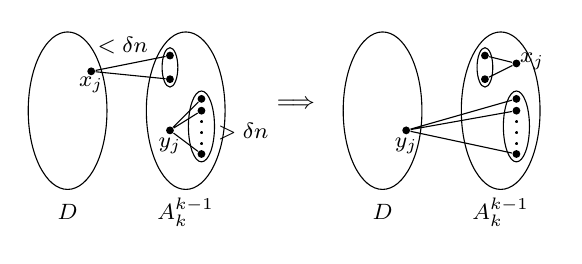
\begin{tikzpicture}[
    node distance=1.5cm,
    set/.style={ellipse, draw, minimum width=1cm, minimum height=2cm},
    smallset/.style={ellipse, draw, minimum width=0.23cm, minimum height=0.9cm},
    label/.style={above, font=\footnotesize},
    point/.style={circle, fill=black, inner sep=1pt},
    box/.style={draw, rectangle, minimum width=5.2cm, minimum height=3cm},
    verysmallset/.style={ellipse, draw, minimum size=0pt,  % 必须先取消默认限制
    inner sep=0pt,     % 取消内边距
    outer sep=0pt, minimum width=0.2cm, minimum height=0.5cm},
]

\node[set, fill=blue!0] (A1) at (2,0) {};
\node[label] at (2,-0.2) {};
\node[label] at (2,-1.5) {$D$};
\node[set, fill=blue!0] (A2) at (3.5,0) {};
\node[label] at (3.5,-0.2) {};
\node[label] at (3.5,-1.6) {$A_k^{k-1}$};
\node[point] (b1) at (2.3,0.5) {};
\node[label] at (2.3,0.1) {$x_j$};
\node[label] at (2.7,0.6) {$<\delta n$};
\node[point] (b2) at (3.3,0.7) {};
\node[point]  (b3) at (3.3,0.4) {};
\node[verysmallset]  (b4) at (3.3,0.55) {};
\draw (b2)--(b1)--(b3);

\node[point] (c1) at (3.3,-0.25) {};
\node[label] at (3.3,-0.67) {$y_j$};
\node[point] (c2) at (3.7,0.15) {};
\node[point] (c3) at (3.7,0) {};
\node[label] at (3.7,-0.57) {$\vdots$};
\node[point] (c4) at (3.7,-0.55) {};
\node[smallset]  (c5) at (3.7,-0.2) {};
\draw (c2)--(c1)--(c3) (c1)--(c4);
\node[label] at (4.23,-0.5) {$>\delta n$};

\node[label] at (4.9,-0.1) {$\Longrightarrow$};

\node[set, fill=blue!0] (A1) at (6,0) {};
\node[label] at (6,-0.2) {};
\node[label] at (6,-1.5) {$D$};
\node[set, fill=blue!0] (A2) at (7.5,0) {};
\node[label] at (7.5,-0.2) {};
\node[label] at (7.5,-1.6) {$A_k^{k-1}$};
\node[point] (b1) at (7.7,0.6) {};
\node[label] at (7.9,0.4) {$x_j$};
%\node[label] at (6.7,0.6) {$<\delta n$};
\node[point] (b2) at (7.3,0.7) {};
\node[point]  (b3) at (7.3,0.4) {};
\node[verysmallset]  (b4) at (7.3,0.55) {};
\draw (b2)--(b1)--(b3);

\node[point] (c1) at (6.3,-0.25) {};
\node[label] at (6.3,-0.67) {$y_j$};
\node[point] (c2) at (7.7,0.15) {};
\node[point] (c3) at (7.7,0) {};
\node[label] at (7.7,-0.57) {$\vdots$};
\node[point] (c4) at (7.7,-0.55) {};
\node[smallset]  (c5) at (7.7,-0.2) {};
\draw (c2)--(c1)--(c3) (c1)--(c4); 
\end{tikzpicture}

    \caption{Vertices $x_j,y_j$ exchanged in the $k$-th step, where 
$\delta=\beta+(k-1)\alpha$ and $D \in \mathcal{P}_{k-1}\setminus{A_k^{k-1}}$.}
    \label{fig:exchang}
\end{figure}


% Let $c_k=a_1+a_2+a_3$, where $a_1$ denotes the number of matching edges in $M_k$ such that both endpoints belong to $A_k\cup X_k'$, $a_2$ denotes the number of matching edges in $M_k$ such that both endpoints belong to $X_k\setminus X_k'$, $a_3$ denote the number of the remaining edges in $M_k$
% . 
% \begin{algorithm}
% \caption{To Get $(r,s)$-neat $(\gamma_s,\gamma_{s+1};S)$-good partition}
% \label{Neat}
% \renewcommand{\algorithmicrequire}{\textbf{Input:}}
% \renewcommand{\algorithmicensure}{\textbf{Output:}}
% \begin{algorithmic}[1]
% \REQUIRE a graph $G$, vertex set $S$, constants $\alpha, \beta$, and $(r,s)$-neat partition $\mathcal{P}$
% \ENSURE An $(r,s)$-neat $(\gamma_s,\gamma_{s+1})$-good partition $\mathcal{Q}$ of $G$
% \FOR{$k=1$ to $s$} 
% \STATE{$X_k=V_{ex}^L(\mathcal{P},\beta, k), Y_k=V_{b}(\mathcal{P},\beta+(k-1)\alpha,k)$ and $H_k=G[A_k\cup X_k]$}
% \WHILE{$X_k\ne \emptyset$ and $Y_k\ne \emptyset$}
% \STATE Pick an $x\in X_k$ and a $y\in Y_k$, move $x$ into $A_k$ and remove $u$ into the part to which $x$ 
% originally belonged
% \STATE $X_k=X_k-x$, $Y_k=Y_k-y$ and $H_k=H_k-x$
% \ENDWHILE
% \IF{$X_k\ne \emptyset$}
% \STATE Find a matching $M_k$ of size $|X_k|$ in $H_k$
% \STATE Adjust the partition such that each matching only has one vertex belonging to $A_k$ and $\mathcal{P}$ is still $(r,s)$-neat
% \ENDIF
% \ENDFOR
% \RETURN the partition $\mathcal{Q}$
% \end{algorithmic}
% \end{algorithm}

%\noindent \textbf{Modifying the partition and covering the large-degree exceptional vertices with disjoint bases}

\begin{claim}\label{A2}
   Either $G$ contains an independent set of size $\frac{n}{r}+1$, or for each $k\in [s]$, there exists an $(r,s)$-partition $\mathcal{P}_k:=\{A_1^k,\ldots,A_s^k,B^k\}$ satisfying  the following.
\begin{enumerate}
[label =\rm  (C\arabic{enumi})]
    \item\label{B01} For each $i\in [s]$, $A_i^k$ is a $(2^k-1)\alpha$-independent set of size $\frac{n}{r}$ in $G$.
    \item\label{B02} If $|B^k| \ge \frac{2n}{r}$, then $G[B^k\setminus S]$ contains no $(\gamma_{s+1}-(2^k-1)\alpha)$-independent set of size $\frac{n}{r}$.
    \item\label{B03} For each $i\in [s]$, we have $$
    |V_b(\mathcal{P}_k,\beta+(2^{k}-1)\alpha, i)|\le 2^k\alpha n\ \text{and}\ |V_{ne}(\mathcal{P}_k,\beta'+(2^k-1)\alpha,i)|\le 2^k\alpha n.
    $$
    \item\label{B05} For each $i\in [k]$, there exists a matching $M_i$ of size $c_i$ in $H_i$ such that  each edge in $M_i$ has exactly one endpoint in $A_i^k$, and $V(M_i)\cap V(M_j)=\emptyset$ for all $i\neq j$. If $M_i\neq \emptyset$, then there are no $(\beta+(2^k-1)\alpha, i)$-bad vertices in $A_i^k$. 
    \item\label{B04}For each $i\in[k]$, there are no $(\beta-(2^k-1)\alpha,i)$-exceptional vertices in $V(G)\setminus (V(H_i)\cup S)$.
%\item[\ref{B05}] If $X_i=\emptyset$ for $1\le i\le k$, we have $V(\mathcal{P}_k,\beta-(\sum_{j=1}^{k}j)\alpha,i)=\emptyset$. If $X_i \ne \emptyset$ for $1\le j\le k$, we have $V(\mathcal{P}_i,\beta+(\sum_{j=1}^{k}j)\alpha,j)=\emptyset$ and there exists a matching $M_i$ such that for each vertex $v\in X_i$, there exists an $e\in M_i$ which covers $v$ and a vertex $u\in A_i$.
\end{enumerate}
%Otherwise, $G$ has an independent set of size $\frac{n}{r}+1$.
\end{claim}

\begin{proof}[Proof of Claim \ref{A2}]
We prove this claim by induction on $k$. We first consider the case that $k=1$. Observe that for each $i\in [s]$, the number of vertices exchanged from $\mathcal{P}_0$ to $\mathcal{P}_1$ within $A_i^1$ (resp. $B^1$) is bounded by $|V_{ex}^L(\mathcal{P}_0,\beta,1)|\le  \alpha n$. Thus, under the partition $\mathcal{P}_1$, for each $i\in[s]$, we have %for each $i\in [s]$ we have 
$$
e(G[A_i^1])\leq \gamma_in^2+\alpha n \cdot \frac{n}{r}\le \alpha n^2,
$$
and for any set $B'\subseteq B^1\setminus S$ of  size $\frac{n}{r}$, we have 
$$
e(G[B'])\ge \gamma_{s+1} n^2-\alpha n\cdot \frac{n}{r}\geq (\gamma_{s+1}-\alpha)n^2.
$$
%the number of edges in $G[A_i]$ is at most $\gamma_sn^2+\alpha n \cdot \frac{n}{r}\le \alpha n^2$, 
Therefore, $A_i^1$ is an $\alpha$-independent set of size $\frac{n}{r}$ for each $i\in [s]$,  and $G[B^1\setminus S]$  contains no  $(\gamma_{s+1}-\alpha)$-independent set of size $\frac{n}{r}$. Hence, \ref{B01} and \ref{B02} hold. %Hence \ref{B01} follows. %     By induction, it is sufficient to show that \ref{B01}-\ref{B05} hold for $k=1$ and if these hold for $k-1$, then these also hold for $k$.
%Let $k=1$. for \ref{B01} and $\rm (I_2)$ with $1\le i \le s$, there are at most $|V_{ex}^L(\mathcal{P},\beta,1)|\le \alpha n$ vertices in $A_i$ exchanged in the $1$st step. Thus the edges of $G[A_i]$ are at most $\gamma_sn^2+\alpha n \cdot \frac{n}{r}\le \alpha n^2$ in the partition $\mathcal{P}_1$, that is, $A_i$ is $\alpha$-independent set of size $\frac{n}{r}$ in $\mathcal{P}_1$. 
%there are at most $|V_{ex}^L(\mathcal{P},\beta,1)|\le \alpha n$ vertices exchanged in $B$. F
%Similarly, in the partition $\mathcal{P}_1$, for any $B'\subseteq B\setminus S$ with size $\frac{n}{r}$, we have $e(G[B'])\ge \gamma_{s+1} n^2-\alpha n\cdot \frac{n}{r}$, that is, $G[B\setminus S]$ does not contain any $(\gamma_{s+1}-\alpha)$-independent set. Hence \ref{B02} holds. 

%Next, for $1\le i \le s$, let us consider $\rm (I_3)$. 
For each vertex $v \in V(G)$, it is straightforward to check that for each $i\in [s]$, 
\begin{align}\label{DV}
    d(v,A_i^0)-\alpha n \le d(v,A_i^1)\le  d(v,A_i^0)+\alpha n.
\end{align}
Therefore, if $v$ is not moved in the first step and $v\notin V_{ne}(\mathcal{P}_0,\beta',i)\cup V_{b}(\mathcal{P}_0,\beta,i)$, then % $v$ is not $(\beta',i)$-excellent (or $(\beta, i)$-bad) in $\mathcal{P}_0$, then 
$v\notin V_{ne}(\mathcal{P}_1,\beta'+\alpha,i)\cup V_{b}(\mathcal{P}_1,\beta+\alpha,i)$. % is not $(\beta'+\alpha, i)$-excellent (or $\beta+\alpha,i)$-bad) in $\mathcal{P}_1$. 
Thus, for each $i\in [s]$ we have 
$$|V_{ne}(\mathcal{P}_1,\beta'+\alpha, i)|\le |V_{ne}(\mathcal{P}_0,\beta',i)|+\alpha n \le 2\alpha n
\text{~and~} |V_{b}(\mathcal{P}_1,\beta+\alpha,i)|\le |V_{b}(\mathcal{P}_0,\beta,i)|+\alpha n \le 2\alpha n.$$
Hence \ref{B03} holds. 

%Finally, we prove \ref{B05}. 
Note that $|V(H_1)|=\frac{n}{r}+c_1$. If $c_1= 1$, then either $H_1$ has a matching $M_1$ of size $c_1$ or $V(H_1)$ is an independent set of size $\frac{n}{r}+1$. %either $V(H)$ is an independent set of size $\frac{n}{r}+1$ in $G$ or $H_1$ has a matching $M_1$ of size $c_1$. For the former case, we terminate the process and output the independent set $V(H)$ of size $\frac{n}{r}+1$. 
If $c_1\ge 2$, then since  $d_G(v)\ge (1-\frac{1}{r})n-1$ for each $v\in V(H_1)$, we have $\delta(G[H_1])\ge c_1-1$.  %Recall that ,  %$Y_1=\emptyset$, we have 
Recall that $H_1=G[(A^0_1\cup X_1)\setminus Y_1]$, \eqref{DV} implies that for each $v\in V(H_1)$ we have 
$$d_{H_1}(v)\le \beta n+|V_{ex}^L(\mathcal{P}_0, \beta,1)|\le (\beta+\alpha)n,$$
 that is, $\Delta(H_1)\le(\beta+\alpha)n$. %If $c_1=1$, then $H_1$ has a matching $M_1$ of size $c_1$ as $G$ contains  no independent set of size $\frac{n}{r}+1$. If $c_1 \ge 2$, then c
 Combining with Lemma~\ref{MStab}, one has that $H_1$ contains a matching $M_1$ of size $c_1$. Notice that 
%$$|M_1\cap E(G[A_1])|=|M_1\cap G[H_1\setminus V(A_1)]|,$$ that is, 
the number of matching edges of $M_1$ within $A_1^0\cup \{x_1^1,\ldots,x_{t_1}^1\}$ is the same as the number of matching edges of $M_1$ within $X_1\setminus \{x_1^1,\ldots,x_{t_1}^1\}$. 
%the number of edges that both endpoints belong to $A_1^0\cup \{x_1^1,\ldots,x_{t_1}^1\}$ is equal to the number of edges that both endpoints belong to $X_1\setminus \{x_1^1,\ldots,x_{t_1}^1\}$. 
Consequently, we can perform vertex exchanges in $V(H_1)$ to ensure that under the partition $\mathcal{P}_1$, every $e \in E(M_1)$ has exactly one endpoint in $A_1^1$ (see Figure~\ref{fig:exchange-matching}). This can be achieved by exchanging at most $c_1$ vertices. %, that is, we exchange at most $c_1$ vertices in this process. 
Furthermore, if $M\ne \emptyset$, then we have $A_1^1\subseteq V(H_1)$, that is, $V_b(\mathcal{P}_1, \beta+\alpha,1)=\emptyset$.
Thus, \ref{B05} holds. 
%  By Lemma \ref{matching}, there is a matching $M_1'$ of size $c_1-1$. Assume that the size of the largest matching in $H_1$ is $c_1-1$. Consider two arbitrary vertices $u,v$ which are not in $M_1'$, there is no edge $xy\in M_1'$ such that $x\in N(u)$ and $y\in N(v)$. Lemma \ref{MStab} implies that $N(u)=N(v)$ for arbitrary $u,v\not \in V(M_1')$. Thus, there is a vertex $v'\in V(M_1')$ such that $$d_{H_1}(v')\ge \frac{n}{r}-2(c_1-1)>(\beta+\alpha)n,$$ contradicting $\Delta(H_1)\le (\beta+\alpha)n$. Therefore, there exists a matching $M_1$ of size $c_1$.
\begin{figure}[ht]
\centering
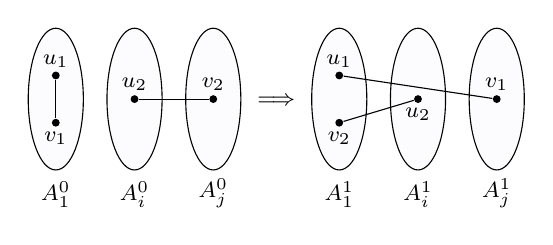
\begin{tikzpicture}[
    node distance=1.5cm,
    set/.style={shape=ellipse, draw, minimum width=0.7cm, minimum height=1.8cm},
    smallset/.style={ellipse, draw, minimum width=0.23cm, minimum height=0.9cm},
    label/.style={above, font=\footnotesize},
    point/.style={circle, fill=black, inner sep=1pt},
    box/.style={draw, rectangle, minimum width=5.2cm, minimum height=3cm},
    verysmallset/.style={ellipse, draw, minimum size=0pt,  % 必须先取消默认限制
    inner sep=0pt,     % 取消内边距
    outer sep=0pt, minimum width=0.2cm, minimum height=0.5cm},
]

\node[set, fill=blue!1] (A1) at (2,0) {};
\node[label] at (2,-1.5) {$A_1^0$};
\node[point] (b1) at (2,0.3) {};
\node[label] at (2,0.28) {$u_1$};
\node[point] (b2) at (2,-0.3) {};
\node[label] at (2,-0.7) {$v_1$};
\node[set, fill=blue!1] (A2) at (3,0) {};
\node[point] (b3) at (3,0) {};
\node[label] at (3,-0.02) {$u_2$};
\node[label] at (3,-1.5) {$A_i^0$};
\node[set, fill=blue!1] (A3) at (4,0) {};
\node[label] at (4,-1.5) {$A_j^0$};
\node[point] (b4) at (4,0) {};
\node[label] at (4,-0.02) {$v_2$};
\draw (b1)--(b2) (b3)--(b4);

\node[label] at (4.8,-0.2) {$\Longrightarrow$};

\node[set, fill=blue!1] (A1) at (5.6,0) {};

\node[label] at (5.6,-1.5) {$A_1^1$};
\node[point] (b1) at (5.6,0.3) {};
\node[label] at (5.6,0.28) {$u_1$};
\node[point] (b2) at (5.6,-0.3) {};
\node[label] at (5.6,-0.7) {$v_2$};
\node[set, fill=blue!1] (A2) at (6.6,0) {};
\node[point] (b3) at (6.6,0) {};
\node[label] at (6.6,-0.4) {$u_2$};
\node[label] at (6.6,-1.5) {$A_i^1$};
\node[set, fill=blue!1] (A3) at (7.6,0) {};
\node[label] at (7.6,-1.5) {$A_j^1$};
\node[point] (b4) at (7.6,0) {};
\node[label] at (7.6,-0.02) {$v_1$};
\draw (b1)--(b4) (b3)--(b2);
\end{tikzpicture}
\caption{Here, $u_1v_1,u_2v_2\in E(M_1)$ with  $u_1,v_1\in A_1^0\cup \{x_1^1,\ldots,x_{t_1}^1\}$, $u_2,v_2\in X_1\setminus \{x_1^1,\ldots,x_{t_1}^1\}$.    
    Exchange $v_1$ and $v_2$ to guarantee that every edge in $M_1$ has exactly one endpoint in $A_1^1$.}
    \label{fig:exchange-matching}
    \end{figure}
%\begin{figure}[ht!]
%    \centering
    %\includegraphics[width=0.45\linewidth]{figure/matching-exchange.pdf}
    %\caption{Here, $u_1v_1,u_2v_2\in E(M_1)$ with  $u_1,v_1\in A_1^0\cup \{x_1^1,\ldots,x_{t_1}^1\}$, $u_2,v_2\in X_1\setminus \{x_1^1,\ldots,x_{t_1}^1\}$.    
    %Exchange $v_1$ and $v_2$ to guarantee that every edge in $M_1$ has exactly one endpoint in $A_1^1$.}
   % \label{fig:exchange-matching}
%\end{figure}

Let $v$ be a vertex in $V(G)\setminus (V(H_1)\cup S)$. If $d(v,A_1^0)\ge \beta n$, then $d(v,A_1^1)\ge (\beta-\alpha)n$, that is, there are no $(\beta-\alpha, i)$-exceptional vertices in $V(G)\setminus V(G)\setminus (V(H_i)\cup S)$ for partition $\mathcal{P}_1$. Thus, \ref{B04} holds.
%Clearly, $v\notin V_{ex}(\mathcal{P}_0,\beta,1)$. If $v$ is not moved in the first step, then \eqref{DV} implies that $v\notin V_{ex}(\mathcal{P}_1,\beta-\alpha, 1)$. If $v$ is moved in the first step, then $v\in V_{b}(\mathcal{P}_0,\beta,1)$ as $v\notin V(H_1)$. Therefore, $v\notin V_{ex}(\mathcal{P}_1,\beta-\alpha, 1)$. %For the latter case, $v\notin V(G)\setminus V(H_1)$. Therefore, 
%Thus, under the partition $\mathcal{P}_1$, there are no $(\beta-\alpha,1)$-exceptional vertices in $V(G)\setminus (V(H_1)\cup S)$, that is, \ref{B04} holds. 
Hence, \ref{B01}-\ref{B04} hold when $k=1$. Next, we assume that \ref{B01}-\ref{B04} hold for $ k-1$, and we will prove that $\mathcal{P}_k$ satisfies all of them. 



%If $v$ is not moved in the first step and $v\notin V_{ex}(\mathcal{P}_0,\beta, 1)$, then \eqref{DV} implies that $v\notin V_{ex}(\mathcal{P}_1,\beta-\alpha, 1)$. % is not $(\beta,1)$-excellent in $\mathcal{P}_0$, then $v$ is not $(\beta-\alpha, 1)$-excellent in $\mathcal{P}_1$. 
%For $i\ne 1$, if $v\in A_i$ in partition $\mathcal{P}_0$ and $v\notin A_i$ in partition $\mathcal{P}_1$, then $v$ is not $(\beta-\alpha,i)$-exceptional, for $v$ is $(\beta,1)$-exceptional in $\mathcal{P}_0$. 
%If $v\in A_1^0$ and $v\notin A_1^1$, then either $v\in V_{b}(\mathcal{P}_0,\beta,1)$ or $v\in V(M_1)$. For the former case, by the inequality \eqref{DV}, we know that $v\notin V_{ex}(\mathcal{P}_1,\beta-\alpha, 1)$. %For the latter case, $v\notin V(G)\setminus V(H_1)$. Therefore, 
%Thus, under the partition $\mathcal{P}_1$, there are no $(\beta-\alpha,1)$-exceptional vertices in $G-(V(H_1)\cup S)$, that is, \ref{B04} holds.  % There are two cases. If $v$ is $(\beta,1)$-bad in $\mathcal{P}_0$, then $v$ is not $(\beta-\alpha,i)$-exceptional. If $v$ is not $(\beta,1)$-bad in $\mathcal{P}_0$, then $v\in H_1$. Further, there are no $(\beta-\alpha,1)$-exceptional vertices in $V(G)\setminus (S\cup H_1).$


% %For \ref{B01} and \ref{B02}, let 
% By induction, we know that %under the partition $\mathcal{P}_{k-1}$, 
% $A_i^{k-1}$ is a $(2^{k-1}-1) \alpha$-independent set and for each $i\in [s]$ one has $$\left|V_{ex}^L(\mathcal{P}_{k-1},\beta+(2^{k-1}-1)\alpha, i)\right|\le 2^{k-1}\alpha n.
% $$
% Hence, at most $2^{k-1}\alpha n$ vertices are exchanged in the $k$-th step. 
%Thus, for each $A_i^k\in \mathcal{P}_k$, we have 
% $$
% e(G[A_i^k])\le (2^{k-1}-1) \alpha n^2+2^{k-1} \alpha n\cdot \frac{n}{r}\le (2^k-1)\alpha n^2, 
% $$
% this implies that $A_i^k$ is a $(2^k-1)\alpha$-independent set. By a similar argument, we obtain that there are no $(\gamma_{s+1}-(2^k-1)\alpha)$-independent sets of size $\frac{n}{r}$ in $G[B^k\setminus S]$. Hence  \ref{B01}-\ref{B02} hold. 

% For each vertex $v \in V(G)$, 
% it is straightforward to check that %For $\rm (I_3)$, let $1\le i \le s$. Since there are at most $2^{k-1} \alpha n$ vertices exchanged in the $k$-th step,  we have 
% \begin{align}\label{DegreeC}
%     d(x,A_i^{k-1})-2^{k-1} \alpha n \le d(x,A_i^k)\le d(x,A_i^{k-1})+2^{k-1} \alpha n.
% \end{align}
% Therefore, if $v$ is not moved in the $k$-th step and $v\notin V_{ne}(\mathcal{P}_{k-1},\beta'+(2^{k-1}-1) \alpha,i)\cup V_{b}(\mathcal{P}_{k-1},\beta+(2^{k-1}-1) \alpha,i)$, then $v\notin V_{ne}(\mathcal{P}_{k},\beta'+(2^{k}-1) \alpha,i)\cup V_{b}(\mathcal{P}_{k},\beta+(2^{k}-1) \alpha,i)$. 
% %is not $(\beta'+(2^{k-1}-1) \alpha,i)$-excellent (or $(\beta+(2^{k-1}-1) \alpha, i)$-bad) in $\mathcal{P}_{k-1}$, then $v$ is not $(\beta'+(2^{k}-1)\alpha, i)$-excellent (or $\beta+(2^{k}-1)\alpha,i)$-bad) in $\mathcal{P}_1$. 
% Thus, by induction we have 
% $$
% |V_{ne}(\mathcal{P}_k,\beta'+(2^{k}-1)\alpha, i)|\le |V_{ne}(\mathcal{P}_{k-1},\beta'+(2^{k-1}-1)\alpha,i)|+2^{k-1} \alpha n \le 2^k\alpha n
% $$
% and
% $$|V_{b}(\mathcal{P}_k,\beta+(2^{k}-1)\alpha,i)|\le |V_{b}(\mathcal{P}_{k-1},\beta+(2^{k-1}-1) \alpha,i)|+2^{k-1}\alpha n \le 2^k\alpha n.$$
% Hence \ref{B03} holds. 

By induction, for each $i\in [s]$, we know that $A_i^{k-1}$ is a $(2^{k-1}-1) \alpha$-independent set and $$\big|V_{ex}(\mathcal{P}_{k-1},\beta,i)\big|\le \big|V_{ne}^L(\mathcal{P}_{k-1},\beta+(2^{k-1}-1)\alpha, i)\big|\le 2^{k-1}\alpha n.
$$
Hence, at most $2^{k-1}\alpha n$ vertices are exchanged in the $k$-th step. Thus, we have 
\begin{align}\label{DegreeC}
    d(x,A_i^{k-1})-2^{k-1} \alpha n \le d(x,A_i^k)\le d(x,A_i^{k-1})+2^{k-1} \alpha n.
\end{align}
By an argument analogous to that for $\mathcal{P}_1$, \ref{B01}-\ref{B03} also hold for $\mathcal{P}_k$. Hence, it remains to prove \ref{B05} and \ref{B04}.
%For \ref{B01}-\ref{B03}, by the same argument used for $\mathcal{P}_1$ also holds for $\mathcal{P}_k$. Thus, it suffices to show $\ref{B05}$ and \ref{B04}.

For \ref{B05}, the same method as for $k=1$ yields an independent set of size $\frac{n}{r}+1$ or a 
matching $M_k$ of size $c_k$ in $H_k$ such that $V_b(\mathcal{P}_k, \beta+(2^k-1)\alpha, k) = \emptyset$ whenever $M_k\neq \emptyset$. By induction, for each $i \in [k-1]$ with $M_i \ne \emptyset$, there are no $(\beta +(2^{k-1}-1)\alpha,i)$-bad vertices in $A_{i}^{k-1}$. Given that \( d(v) \ge \left(1 - \frac{1}{r}\right)n - 1 \) for every \( v \in V(G) \setminus S \), and by Fact~\ref{ExFact}, it follows that no vertex  in \(A_i \) is exchanged in the \( k \)-th step. Therefore, \( V_b\bigl(\mathcal{P}_k, \beta + (2^k - 1)\alpha, i\bigr) = \emptyset \), and every edge in \( M_i \) has exactly one endpoint in \( A_i^k \). %Combining with Fact \ref{ExFact}, since $d(v)\ge (1-\frac{1}{r})n-1$ for any $v\in V(G)\setminus S$, no vertices $v\in A_i^{k-1}$ are exchanged in the $k$-th step, that is, $V_b(\mathcal{P}_k, \beta+(2^k-1)\alpha, i) = \emptyset$ and each edge in $M_i$ has exactly one endpoint in $A_i^k$. 
Moreover, by induction, the inequality \eqref{DegreeC} implies that 
$$d(x_i,A^k_i)\le (\beta+(2^{k-1}-1)\alpha)n+2^{k-1}\alpha n\le (\beta+(2^k-1)\alpha) n$$ 
for each $i \in [k-1]$ and each $x_i\in V(H_i)$. For $H_k$ with any $x_k\in V(H_k)$, we have 
$$d(x_k,A^k_k)\le (\beta+(k-1)\alpha)n+2^{k-1}\alpha n\le (\beta+(2^k-1)\alpha )n.$$
Combining with Fact \ref{ExFact}, since $d(v)\ge (1-\frac{1}{r})n-1$ for any $v\in V(G)\setminus S$, we have that $V(H_i)\cap V(H_j)=\emptyset$ for all $i\ne j\in [k]$, which implies  $V(M_i)\cap V(M_j)=\emptyset$ for all $i\ne j\in [k]$. Thus, \ref{B05} holds.

By a similar argument, we have that there are no $(\beta-(2^{k}-1)\alpha,k)$-exceptional vertices in $V(G)\setminus(V(H_k)\cup S)$. For each $i\in [k-1]$, let $v\in V(G)\setminus (V(H_i)\cup S)$. By induction, we have $d(v,A_i^{k-1})\ge (\beta -(2^{k-1}-1)\alpha)n$. Thus, \eqref{DegreeC} implies that 
$$d(v,A_i^{k})\ge (\beta -(2^{k-1}-1)\alpha)n-2^{k-1}\alpha n\ge (\beta-(2^{k}-1)\alpha)n.$$ Hence, \ref{B04} holds. %. Let us consider $i\in [k-1]$. Assume $v\in V(G)\setminus(V(H)\cup S)$ and $d(v,A^k_i)\le (\beta-(2^{k}-1)\alpha)n$. The inequality \eqref{DegreeC} implies that $d(v,A^{k-1}_i)\le (\beta-(2^{k-1}-1)\alpha)n$. By induction, we have that $v\in H_i$. Since $V(H_i)\cap V(H_j)=\emptyset$ for all $i\ne j$, Fact \ref{ExFact} implies that \ref{B04} holds.
% Notice that %under  $\mathcal{P}_{k-1}$, 
% $d(u,A_i^{k-1})\le (\beta+(2^k-1)\alpha) n$ for every $u\in V(H_i)$ with $i\in [k-1]$. Fact \ref{ExFact} implies that $H_i\cap X_k=\emptyset$, that is, every $u\in V(H_i)\cap A_i^{k-1}$ with $i\in [k-1]$ is not moved in the $k$-th step and every vertex $v\in V(H_i)\setminus A_i^{k-1}$ does not belong to $A_i^{k}$.
% Hence $H_1, \dots, H_k$ are vertex-disjoint. For each $i\in [k-1]$, by induction, there are no $(\beta-(2^{k-1}-1)\alpha,A_i^{k-1})$-exceptional vertices in  $V(G)\setminus(S\cup V(H_i))$. Together with \eqref{DegreeC}, we know that for each $i\in [k]$,  $V(G)\setminus(S\cup V(H_i))$ contains no $(\beta-(2^{k}-1)\alpha,A_i^k)$-exceptional vertices. Hence \ref{B04} follows. 
\end{proof}
% For $i=k$, 
% if $v$ is not moved the $k$-th step and $v$ is not $(\beta,k)$-excellent in $\mathcal{P}_{k-1}$, then $v$ is not $(\beta-(2^{k}-1)\alpha, i)$-excellent in $\mathcal{P}_k$. If $v\in A_k$ in partition $\mathcal{P}_{k-1}$ and $v\notin A_k$ in partition $\mathcal{P}_k$, then there are two cases. If $v$ is $(\beta+(2^{k-1}-1) \alpha,k)$-bad in $\mathcal{P}_{k-1}$, then $v$ is not $(\beta-\alpha,k)$-exceptional. If $v$ is not $(\beta+(2^{k-1}-1) \alpha,k)$-bad in $\mathcal{P}_{k-1}$, then $v\in H_k$. Further, there are no $(\beta-\alpha,1)$-exceptional vertices in $V(G)\setminus (S\cup H_k).$

% we adjust at most $\alpha n$ vertices in each step. Therefore, for each vertex and any $1\le i,k \le r$, we have 

% For $M_k$, if there exists a vertex $x\in G\setminus(V(H_k)\cup S)$ is $(\beta-k\alpha,k)$-exceptional, then $d(x,A_k)\le (\beta-(k-1)\alpha) n$ in the partition $\mathcal{P}_{k-1}$, that is, $x$ is $(\beta,i)$-exceptional or $(\beta,i)$-good in the partition $\mathcal{P}_{k-1}$. It is a contradiction to our process.

% For $1\le i\le k-1$, if there exists a vertex $x\in G\cup S)$ is $(\beta-k\alpha,i)$-exceptional, then $d(x,i)\le (\beta-(k-1)\alpha)n$ in the partition $\mathcal{P}_{k-1}$. If $x \notin H_{k-1}$, it is a contradiction to $\rm (I_4)$.
% For $A_k$, if $|H_k|>\frac{n}{r}$ after the $k$-th for loop, then we have $\Delta(G)\le \beta+k\alpha$. Thus, there is not $(\beta+k\alpha,k)$-bad vertices. If $|H_k|=\frac{n}{r}$ after the $k$-th for loop, then there is not $(\beta-\alpha,k)$-exceptional vertices. 

% For $1\le i\le k-1$, assume that there exist two vertices $x,y\in V(G)\setminus S$, where $x$ is $(\beta-k\alpha,i)$-exceptional and $y$ is $(\beta+k\alpha,i)$-bad after the $k$-th for loop. Since $d(x)\ge (1-\frac{1}{r})n-1$, there exists most one part $A_\ell$, where $1\le \ell \le r$, such that $d(x,A_\ell)\le \frac{n}{2r}-1$. Therefore, $x$ is $(\beta-(k-1)\alpha, i)$exceptional after the $k-1$th for loop. \eqref{DegreeC} implies that $d(y, i)\ge (\beta+(k-1)\alpha)n$. Vertex $y$ is in $A_k$ after the $k-1$th for loop. Otherwise, $x$ is $(\beta-(k-1)\alpha, \ell)$-exceptional and $(\beta+(k-1)\alpha, \ell)$-bad, contradicting \ref{B05}. By algorithm, there exists a vertex $z\in A_\ell$, which is $(\beta, k)$-exceptional after the $k-1$ for loop, to move $y$ into $A_\ell$. But, $d(z,A_i)\ge \frac{n}{r}-(\beta-(k-1)\alpha)n> \frac{n}{2r}-1$, that is, $z$ is $(\beta+(k-1)\alpha,i)$-bad after the $k-1$ for loop, contradicting to \ref{B05}. 

%By the similar argument of \ref{B05} for $k=1$, there exists a matching $M_i$ of size $|X_i|$ satisfying the condition for $2 \le i \le r$.
%\end{proof}

%Let $X_1:=V_{ex}^L(\mathcal{P},\beta,1), Y_1:=V_b(\mathcal{P},\beta,1)$ and $H_1:=G[A_1\cup V_{ex}^L(\mathcal{P},\beta,1)]$. Let us do the following process. For each vertex $v\in X_1$, let us choose a vertex $u\in Y_1$. Move $v$ into $A_1$ and remove $u$ into the part to which $v$ originally belonged. Let $X_1:=X_1-v,Y_1:=Y_1-u$, and $H_1=H_1-u$. Repeat the upper process until $X_1=\emptyset$ or $Y_1=\emptyset$. If $X_1=\emptyset$, terminate this process. If $Y_1=\emptyset$ but $X_1 \ne \emptyset$, let find a matching $M_1$ of size $c_1:=|X_1|$ in $H_1$ and adjust the vertices of $H_1$ such that one endpoint belongs to $A_1$ and another  belongs to $X_1$ for each edge of matching $M_1$ and $A_1,\ldots, A_s, B$ is still an $(r,s)$-neat partition $\mathcal{P}_1$. Let us call the above process \textit{Step $1$}. After Step $1$, we have that:
%\begin{itemize}
%\setlength{\parskip}{0pt}
    %\item[$(1.1)$] For $0\le i \le s$, $A_i$ is an $\alpha$-independent set of size $\frac{n}{r}$ in $G$ in the partition $\mathcal{P}_1$.
    %\item[$(1.2)$] If $B \ne \emptyset$, then $G[B]$ does not contain any $(\gamma_{s+1}-\alpha)$-independent set of size $\frac{n}{r}$.
    %\item[$(1.3)$] For $1\le i \le s$, we have $|V_b(\mathcal{P}_1,\beta+\alpha,i)|\le 2\alpha n$ and $|V_{ex}(\mathcal{P}_1,\beta-\alpha,i)|\le 2\alpha n$.
%     \item[$(1.4)$] For $1\le i\le s$, we have $|V_{ne}(\mathcal{P}_1,\beta'+\alpha,i)|\le 2\alpha n$.
%     \item[$(1.5)$] If $X_1=\emptyset$, we have $V_{ex}^L(\mathcal{P}_1,\beta'-\alpha,1)=\emptyset$. If $X_1 \ne \emptyset$, we have $V_b(\mathcal{P}_1,\beta'+\alpha,1)=\emptyset$ and there exists a matching $M_1\subseteq H_1$ such that for each vertex $v\in X_1$, there exists an $e\in M_1$ which covers $v$ and a vertex $u\in A_1$.
% \end{itemize}
% 由于A_1的变化，这里$V_{ex}^L(\beta,i)$,A_i等符号存在表述不清楚的问题。




% Based on the partition after Step 1, the following similar process is called \textit{Step $2$}. Let $X_2:=V_{ex}^\ell (\mathcal{P}_1, \beta,2), Y_2:=V_b(\mathcal{P}_1, \beta+\alpha,2)$ and $H_2:=G[A_2\cup V_{ex}^L(\mathcal{P}_1,\beta,2)]$. Let us do the following process. For each vertex $v\in X_2$, pick a vertex $u\in Y_2$. Move $v$ into $A_2$ and remove $u$ into the part to which $v$ originally belonged. Let $X_2:=X_2-v,Y_2=Y_2-u$ $H_2=H_2-u$. Repeat the upper process until $X_2=\emptyset$ or $Y_2=\emptyset$. If $X_2=\emptyset$, terminate this process. If $Y_2=\emptyset$ but $X_2 \ne \emptyset$, let find a matching $M_2$ of size $c_2:=|X_2|$ and adjust the vertices of $H_2$ such that one endpoint belongs to $A_2$ and another  belongs to $X_2$ for each edge of matching $M_2$ and $A_1,\ldots, A_s, B$ is still an $(r,s)$-neat partition $\mathcal{P}_2$. After the Step $2$, we have:
% \begin{itemize}
% \setlength{\parskip}{0pt}
%     \item[$(2.1)$] For $0\le i \le s$, $A_i$ is an $3 \alpha$-independent set of size $\frac{n}{r}$ in $G$.
%     \item[$(2.2)$] If $B \ne \emptyset$ the $G[B]$ does not contain any $(\gamma_{s+1}-3\alpha)$-independent set of size $\frac{n}{r}$.
%     \item[$(2.3)$] For $1\le i \le s$, We have $|V_b(\mathcal{P}_2,\beta+3\alpha, i)|\le 4\alpha n$ and $|V_{ex}(\mathcal{P}_2,\beta-3\alpha,i)|\ge 4\alpha n$.
%     \item[$(2.4)$] For $1\le i\le s$, we have $|V_{ne}(\mathcal{P}_2,\beta'+3\alpha,i)|\le 4\alpha n$.
%     \item[$(2.5)$] If $X_i=\emptyset$ for $i=1,2$, we have $V(\mathcal{P}_2,\beta-3\alpha,i)=\emptyset$. If $X_i \ne \emptyset$ for $1=1,2$, we have $V(\mathcal{P}_2,\beta+3\alpha,i)=\emptyset$ and there exists a matching $M_i\subseteq H_i$ such that for each vertex $v\in X_i$, there exists an $e\in M_i$ which covers $v$ and a vertex $u\in A_i$.
% \end{itemize}
% For $(2.1)$-$(2.4)$, the arguments are similar with Step $1$. For $(2.5)$, if a vertex $x\in A_2$ was initially $(\beta+\alpha,2)$-good, then after Step $2$, $x$ is $(\beta+3\alpha,2)$-good or $(\beta+3\alpha, 2)$-exceptional. Similarly, if a vertex $y\in V(G)\setminus (A_2\cup S)$ was $(\beta,2)$-acceptable after Step $1$, then after Step $2$, $y$ is still $(\beta-2\alpha,2)$-acceptable. Assume $v$ does not belong to a matching edge, we have that if $v\in A_2$ before Step $2$ and $v\not \in A_2$ after Step $2$, then $v$ is not $(\beta-2\alpha,2)$-exceptional vertex. If $v \not \in A_2$ before Step $2$ and $v\in A_2$ after Step $2$, then $v$ is not $(\beta+3\alpha,2)$-bad vertex. Further, there are no $(\beta+3\alpha,2)$-good vertices or there are no $(\beta-3\alpha,2)$-bad vertices after step $2$.

% Recall that after Step $1$ there are no $(\beta+\alpha,1)$-bad vertices in $A_1$ or there is no $(\beta-\alpha,1)$-exceptional vertices in $V(G)\setminus (A_1\cup S)$. Suppose that the former holds. Since $d(v)\ge (1-\frac{1}{r})n-1$ for $v
% \in A_1$, we have $d(v, A_2)\ge |A_2|-(\beta+\alpha)n-1$, that is, $v$ is not $(\beta,2)$-exceptional. In particular, $A_1$ is not modified in Step $2$. Next, suppose that the latter holds. Assume that $x$ is a vertex in $V(G)\setminus (A_1 \cup S)$ after Step $1$ and Step $2$. After Step $2$, $x$ is a $(\beta-3\alpha,1)$-acceptable vertex. Suppose that $x$ is a vertex in $A_1$ after Step $1$ and a vertex in $V(G)\setminus (A_1 \cup S)$ after Step $2$. Then $x\in A_2$ after Step $2$ and so was a $(\beta,2)$-exceptional vertex after Step $1$. Since $d(x)\ge (1-\frac{1}{r})n-1$,  $x$ is a $(\beta+2\alpha, 1)$-excellent vertices after Step $2$ (in particular, $x$ is not $(\beta-3\alpha,1)$-exceptional). Overall this indicates that there are no $(\beta+3\alpha,1)$-bad vertices in $A_1$ or are no $(\beta-3\alpha,1)$-exceptional vertices in $V(G)\setminus (A_1 \cup S)$. By the same argument after Step $1$, there exists a matching of size $c_2$.

% By applying an analogous switching procedure iteratively for $A_3,\ldots,A_s$, we get an $(n,s)$-neat partition $\mathcal{Q}$ such that the following conditions hold:
% \begin{itemize}
% \setlength{\parskip}{0pt}
%     \item[($\alpha_1$)] $S\subseteq B$ and $A_i$ is an $\sqrt{\alpha}$-independent set of size $\frac{n}{r}$ in $G$ for all $0\le i \le s$.
%     \item[($\alpha_2$)] If $B \ne \emptyset$ the $G[B]$ does not contain any $(\frac{\gamma_{s+1}}{2})$-independent set of size $\frac{n}{r}$.
%     \item[($\alpha_3$)] For $1\le i \le s$, we have $|V_b(\mathcal{Q},2\beta,i)|\le \sqrt{\alpha}n$ and $|V_{ex}(\mathcal{Q},\beta/2,i)|\le \sqrt{\alpha} n$.
%     \item[($\alpha_4$)] For $1\le i\le s$, we have $|V_{ne}(\mathcal{Q},2\beta',i)|\le \sqrt{\alpha}n$.
%     \item[($\alpha_5$)] For each $1\le i\le s$, if $V(H_i)\setminus A_i=\emptyset$, there are not $(\beta/2, i)$-exceptional vertices. If $V(H_i)\setminus A_i\ne \emptyset$, there are not $(2\beta, i)$-bad vertices in $A_1$ and there exists a matching $M_i\subseteq H_i$ such that for each vertex $v\in V(H_i)\setminus A_i$, there exists an $e\in M_1$ that covers $v$ and a vertex $u\in A_i$.
% \end{itemize}

By Claim \ref{A2}, either $G$ has an  independent set of size $\frac{n}{r}+1$, or it admits an $(r,s)$-good partition. In the former case, the proof is complete. We may thus assume the latter, and let $\mathcal{Q}:=\{A_1,\ldots,A_s,B\}$ be the partition $\mathcal{P}_s$ obtained by Claim \ref{A2}. We will show that $\mathcal{Q}$ is the desired good partition. Clearly, \ref{B1} follows by \ref{B01} and the fact that $(2^s-1)\alpha \le \sqrt{\alpha}$. By \ref{B05}, there exist $s$ vertex-disjoint matchings $M_1,\dots, M_s$. %Let $M_i':=\{uv\in M_i: u\in V_{ex}^L(\beta/2)\}$. 
 Thus \ref{B05} and \ref{B04} implies \ref{B4}.

It is routine to check that for two constants  $\mu_1,\mu_2$ with  $\mu_1\le \mu_2$, for each $i\in [s]$ we have  
$$
|V_{ne}(\mu_1,i)|\ge |V_{ne}(\mu_2,i)|,\,|V_{b}(\mu_1,i)|\ge |V_{b}(\mu_2,i)|\ \text{and}\ |V_{ex}(\mu_2,i)|\ge |V_{ex}(\mu_1,i)|.
$$ 
Hence, \ref{B3} holds  by \ref{B03}.

Finally, we prove \ref{B2} by considering the following two cases: $|B\setminus S|\ge \frac{n}{r}$ and $|B\setminus S| < \frac{n}{r}$. We start with $|B\setminus S| \ge \frac{n}{r}$. Let $B' \subseteq B$ be an arbitrary  subset of size $\frac{n}{r}$,  %that induces the fewest edges in $G[B']$ among all such  possible subsets of $B$, 
and let $C\subseteq B\setminus (S\cup B')$ be a set with size $|B'\cap S|$. If $|B'\cap S|\geq \gamma_{s+1}n$, then 
$$
e(G[B'])\geq e(G[B' \cap S])\geq \frac{\gamma_{s+1}^2}{4}n^2.
$$
If $|B'\cap S|<\gamma_{s+1}n$, then 
\begin{align*}
    e(G[B'])-e(G[(B'\setminus S)\cup C])&\geq e(G[B'\setminus S,B'\cap S])-e(G[B'\setminus S,C])\geq -|B'\setminus S||C|\geq -\frac{n}{r}\cdot \gamma_{s+1}n.
\end{align*}
Therefore, by \ref{B02} we have 
$$
e(G[B'])\geq e(G[(B'\setminus S)\cup C])-\frac{n}{r}\cdot \gamma_{s+1}n\geq (\gamma_{s+1}-(2^s-1)\alpha)n^2-\frac{n}{r}\cdot \gamma_{s+1}n 
    \geq \frac{\gamma_{s+1}^2}{4}n^2.
$$
That is, $B'$ is not a $\frac{\gamma_{s+1}^2}{4}$-independent set in $G$. 


%e(G[(B'\setminus S)\cup C])=e(G[B'\setminus S])+e(G[C]) +e(B'\setminus S,C)\ge  (\gamma_{s+1}-(2^s-1)\alpha)n^2\ge \frac{\gamma_{s+1}}{2}n^2.

%{\color{red}If, for all edge $e\in E(G[B'])$, one endpoint lies in $C$, then there are at least $\frac{\gamma_{s+1}}{2}n$ vertices contained in $C$.} Since 
%$$
%e([B'])=e(G[B'\setminus S])+\binom{|B'\cap S|}{2} +e(B'\setminus S,B\cap S)\ge e(G[B'\setminus S])+\binom{|B'\cap S|}{2},
%$$
%we obtain $e(G[B'])\ge \frac{\gamma_{s+1}^2}{4}n^2$.

Now, we consider that $|B\setminus S|<\frac{n}{r}$. It is easy to see that if $|B\setminus S|\leq \frac{n}{2r}$, then \ref{B2} holds immediately. Hence we may assume that $|B\setminus S|> \frac{n}{2r}$ in the following. Since $|B|\ge \frac{2n}{r}$, we obtain $|S|> \frac{n}{r}$. Let $v$ be a vertex in $S$. If  $v$ is $(2\beta',i)$-excellent for all $i\in [s]$, then $d(v,B\setminus S)<2r \beta' n$, as $d(v)< (1-\frac{1}{r})n -2$. It follows that %Since $|\cup_{i=1}^{s}V_{ne}(2\beta',i)|\le r \cdot \sqrt{{\alpha}}n$, we have that
$$e(G[B\setminus S,S])\le d(v,B\setminus S)\cdot |S|+|B\setminus S|\cdot \Big|\bigcup_{i\in [s]}V_{ne}(2\beta',i)\Big|\leq 2r\beta' n\cdot |S|+\frac{n}{r}\cdot r  \sqrt{{\alpha}}n=2r\beta' n\cdot |S|+\sqrt{{\alpha}}n^2.$$
% Thus, there exists a vertex $x\in B\setminus S$ such that $d(x, S)\leq \beta n$. Since $d(x)\ge(1- \frac{1}{r})n-1$,  %for any $x\in B\setminus S$, 
% we have 
% $$
% \frac{n}{r}>|B\setminus S|\geq d(x,B\setminus S)\geq \left(1- \frac{s+1}{r}\right)n-1-\beta n.
% $$
% It follows that $r-s=2$ and $|B\setminus S|\geq \frac{n}{r}-\beta n-1$. 
Thus, we obtain that
\begin{align*}
    2e(G[B\setminus S])&\geq \Big(\big(1-\frac{1}{r}\big)n-1-\frac{r-2}{r}n\Big)|B\setminus S|-e(G[S,B\setminus S])\\
    &\geq \Big(\frac{n}{r}-1\Big)\frac{n}{2r}-2r\beta'n \Big(\frac{n}{r}+\beta n+1\Big)-\sqrt{\alpha}n^2\\
    &\geq \frac{\gamma_{s+1}^2}{2}n^2.
\end{align*}
Therefore, any subset of $B$ with size $\frac{n}{r}$ is not a $\frac{\gamma_{s+1}^2}{4}$-independent set in $G$. Hence \ref{B2} holds. 
%we have  $\delta(G[B\setminus S])\ge (1-\frac{s+1}{r})n-\beta n.$ If $r-s\ge 3$, then $\delta(G[B\setminus S])>\frac{n}{r}$, a contradiction. If $r-s=2$, t
%Then $d(G[B\setminus S])\ge \frac{n}{r}-\beta n$, that is $e(G[B\setminus S])> \frac{n^2}{4r^2}\gg \frac{\gamma_{s+1}^2}{4}n^2.$ Combine the arguments of $|B\setminus S|\ge\frac{n}{r}$ and $|B\setminus S|<\frac{n}{r}$ for $|B|\ge \frac{2n}{r}$, $\rm (ii)$ holds.
 % For $\rm (iv)$, the conditions $\rm (I_4)$ and \ref{B05} imply that there exists a matching $M_i'\subseteq M_i$ covering $V_{ex}^L(\mathcal{Q}, \beta/2,i)$ and the edge $e\in M_i'$ satisfying the condition in $\rm (iv)$.
\end{proof}

% Next, let us focus on the $(r,s)$-neat $(\gamma_{s},\gamma_{s+1})$-partition $\mathcal{Q}$.

% \begin{align}\label{OreinB}
%     \sigma(G[B])\ge 2(1-\frac{1}{r-s})|B|-2.
% \end{align}



%\begin{definition}
%Given integers $n,r,t,s$ and a constant $\xi$ with $n\gg r\ge 3$ and $t,\xi>0$, let $G$ be an $n$-vertex graph and $\mathcal{P}$ be an $(r,s)$-partition of $G$. A \textit{$(t,\xi)$-base} is a subgraph $H$ of $G$ with $t$ components such that for each component $C$, the following hold:
%\begin{enumerate}
%[label =\rm  (C\arabic{enumi})]
%    \item\label{C1} There are at least $s$ parts $D\in \mathcal{P}$ satisfying 
%\begin{align}\label{Tdegree}
%   |N(C)\cap D|\ge |D|-(|C\cap D|+1)\frac{n}{r} +\xi n.
%\end{align}
%    \item\label{C2} For each $D\in \mathcal{P}$, $|C\cap D|\le \frac{r|D|}{n}+1,$ with equality holding for at most one $D\in \mathcal{P}$.
%\item\label{C3} For each $i\in [s]$, define $a_i:=|\{C:|C\cap A_i|=2\}|$ and $b:=|\{C:|C\cap B|=r-s+1\}|$. Then $\sum_{i=1}^{s}a_i=b$.
%\end{enumerate}
%\end{definition}


%The condition \ref{C1} is the key condition to get the $K_r$ factor. The conditions \ref{C2} and \ref{C3} help us to ensure that the partition $\mathcal{P}$ on the remaining graph is still an $(r,s)$-partition. 

% \red{Let $B_1\vee B_2\subseteq B$. A $(2, \xi)$-base $H$ with two components $C_1,C_2$ is \textit{balanced} for $B_1\vee B_2$ if there is some $i$ such that $|N(C_1)\cap B_i| \ge \frac{\xi}{8}n$ and $V(C_2) \subseteq B_i$.}

% \begin{proposition}
%     Assume that %\delta_1,\delta_2$ be two constants with 
%     $0<\gamma_s\ll \delta_1 \ll \delta_2\ll \gamma_{s+1}$ and $G$ is an $n$-vertex graph with $\sigma(G)\ge 2(1-\frac{1}{r})n-2$. Let  $\mathcal{Q}$ be an $(r,s;\gamma_s,\gamma_{s+1};S)$-good partition of $G$. If $\mathcal{H}$ is a $(2,\delta_2)$-base set of size $\delta_1 n$, then $G$ admits a $K_r$-tiling $T$ satisfying the following. 
% \begin{itemize}
%     \item[$\rm (i)$] Every $H \in \mathcal{H}$ is contained in at most $2$ copies of $K_r$ in $T$.
%     \item[$\rm (ii)$] The partition $\mathcal{Q}'$ of $G-T$, derived from $\mathcal{Q}$ by deleting all vertices in $T$, preserves the $(r,s;2\gamma_s,\gamma_{s+1}/2;S')$-balanced property, where $S'=S\setminus V(T)$. 
%  %The partition $\mathcal{Q}'$ of $G-T$, obtained from $\mathcal{Q}$ by removing all vertices $T$, remains an $(r,s;2\gamma_s,\gamma_{s+1}/2;S')$-good partition, where $S'$ is obtained from $S$ by removing the vertices in $T$.
% \end{itemize}
% \end{proposition}

% \begin{proof}[\bf Proof]
    
% \end{proof}




\section{Proof of Lemma \ref{K_r-tiling}}\label{section7}

% In this section, let $G$ be an arbitrary $n$-vertex graph with $\sigma(G)\ge 2(1-\frac{1}{r})n-2$ and no independent set of size $\frac{n}{r}+1$, which admits an  $(r,s;\gamma_s,\gamma_{s+1};S)$-good partition $\mathcal{Q}=\{A_1,\ldots,A_s,B\}$ of $G$ for some $s\in [r]$, where $S:=\{x\in V(G):d(x)<(1-\frac{1}{r})n-1\}$. %Let $\mathcal{Q}$ be an $(r,s;\gamma_s,\gamma_{s+1};S)$-good partition of $G$.

With a good partition of $G$ provided by Lemma~\ref{Lpartition}, our task in this section is to
%Lemma \ref{Lpartition} gives a good partition of $G$.  In this section, we aim to 
construct a $K_r$-tiling that covers all non-excellent vertices under the partition. Throughout, we assume the following hypothesis:

\begin{enumerate}
[label =$(\dag)$]
    \item\label{assumption} Given the parameters defined in \eqref{eq:p1}-\eqref{eq:p3}, let $G$ be an $n$-vertex graph with
$\sigma(G)\ge 2\left(1-\frac{1}{r}\right)n-2$ 
and suppose $G$ has a $\gamma$-independent set of size $\frac{n}{r}$. Let $\mathcal{Q}:=\{A_1,\ldots,A_s,B\}$ be an $(r,s;\gamma_s,\gamma_{s+1};S)$-good partition of $G$ for some $s\in[r]$, where $S:=\{x\in V(G):d(x)<(1-\frac{1}{r})n-1\}.$
\end{enumerate}


We first define some necessary notation and provide several properties of the $(r,s;\gamma_s,\gamma_{s+1}; S)$-good partition $\mathcal{Q}$. Define 
\begin{align*}
    &V_{ex}(\beta):=\bigcup_{i=1}^{s}V_{ex}(\beta,i),\ V_{ex}^S(\beta):=V_{ex}(\beta)\cap S\ \text{and}\ V_{ex}^L(\beta):=V_{ex}(\beta)\setminus V_{ex}^S(\beta);\\
    &V_e{(2\beta')}:=\bigcap_{D\in \mathcal{Q}} (V_e(2\beta',D)\cup D),\ V_e^S{(2\beta')}:=V_e{(2\beta')}\cap S\ \text{and}\ V_e^L{(2\beta')}:=V_e{(2\beta')}\setminus V_e^S{(2\beta')}.
\end{align*}
Let $V_{ne}(2\beta'):=V(G)\setminus V_e(2\beta')$.  
We claim that 
$$
|V_{ne}(2\beta',B)|\le \alpha^{1/4} n.
$$
Otherwise, suppose that $|V_{ne}(2\beta',B)|> \alpha^{1/4} n$. By the Pigeonhole Principle, there exists some $i\in [s]$ such that there are at least $\frac{\alpha^{1/4} n}{s}$ vertices $v\in A_i$ satisfying $d(v,B)<|B|-2\beta' n$. Since $d(v)\ge (1-\frac{1}{r})n-1$ for each $v\in A_i$, we obtain that 
$$|E(G[A_i])|\geq \frac{1}{2}\cdot\frac{\alpha^{1/4} n}{s} \cdot (2\beta'n-1)\ge \sqrt{\alpha}n^2,$$ 
which contradicts \ref{B1} of Definition \ref{Partition}. Combining with \ref{B3}, we get
\begin{align}\label{size-of-ne}
    |V_{ne}(2\beta')|\leq 2\alpha^{1/4}n.
\end{align}





To prove Lemma \ref{K_r-tiling}, we employ a critical structure, called a \textit{base}, that covers all non-excellent vertices and whose extension property ensures the existence of a vertex-disjoint $K_r$-tiling.%which possesses a key extension property that can be extended to disjoint $K_r$ copies. % that facilitates this covering.

%Aim: to find a $K_r$-tiling in \ref{K_r-tiling} covering `not excellent' vertices, we see a smaller structure, `base', with a good property of extension. 

\begin{definition}[Base]\label{Base}
Given integers $n,r,s$  with $n\gg r\ge 3$ and a positive constant $\xi$, let $G$ be an $n$-vertex graph and $\mathcal{P}$ be an $(r,s)$-partition of $G$. 
\begin{itemize}
    \item We say a clique $C$ is a \textit{$\xi$-base} in $G$ if for each  $D\in\mathcal{P}$ we have 
\begin{enumerate}
[label =\rm  (D\arabic{enumi})]
    \item\label{C01} $|V(C)\cap D|\le \frac{r|D|}{n}$,
    \item\label{C02}  $|N(V(C))\cap D|\ge |D|-(|V(C)\cap D|+1)\cdot \frac{n}{r} +\xi n$.
\end{enumerate}

\item We say a pair of vertex-disjoint cliques $C_0$ and $C_1$ is a \textit{$(2,\xi)$-base} in $G$ if there exist two  different parts $D_0, D_1\in \mathcal{P}$ satisfying the following conditions.
\begin{enumerate}
[label =\rm  (D\arabic{enumi})]
\addtocounter{enumi}{2}
    \item\label{C03} For each $i\in\mathbb{Z}_2$, we have $|V(C_i)\cap D_i|=\frac{r|D_i|}{n}+1$ and  $|V(C_i)\cap D|\le \frac{r|D|}{n}$ for each $D\in \mathcal{P}\setminus\{D_{i}\}$.
    \item\label{C04} For each $i\in \mathbb{Z}_2$, \ref{C02} holds for all $D\in \mathcal{P}\setminus \{D_{i+1}\}$, and 
    $$|N(V(C_i))\cap D_{i+1}|\ge |D_{i+1}|-(|V(C)\cap D_{i+1}|+2)\cdot \frac{n}{r}+\xi n.$$
\end{enumerate}
\end{itemize}
\end{definition}

A collection $\mathcal{H}$ of vertex-disjoint subgraphs of $G$ is called a \textit{$\xi$-base set} if for each $H \in \mathcal{H}$, there exists a parameter $\tau \geq \xi$ for which $H$ is either a $\tau$-base or a $(2, \tau)$-base. % for some $\tau \ge \xi.$ 
Here, \ref{C02} and \ref{C04} provide the fundamental criterion for extending a base structure to a copy of $K_r$, while \ref{C01} and \ref{C03} ensure that after extending the base set to a $K_r$-tiling, the partition $\mathcal{P}$ retains its $(r,s)$-partition property in the remaining graph.


In the following, we split the proof of Lemma \ref{K_r-tiling} into two parts. In Section \ref{section7.1}, we construct a $\beta/4$-base set that covers all vertices in $V_{ne}(2\beta')$. In Section \ref{section7.2}, we extend the base set to a $K_r$-tiling satisfying \ref{L2}. %These two steps are addressed in the following subsections.

\subsection{Covering vertices in  $V_{ne}(2\beta')$}\label{section7.1}


%into three disjoint subsets: $V_{ex}^L(\beta/2)$, $V_{ex}^S(\beta/2)$, and $V_{ne}(2\beta')\setminus V_{ex}(\beta/2)$. 
Denote  $|V_{ex}^S(\beta/2,i)|=s_i$ for each $i\in [s]$. Let $f(x,y)$ be a function of $x$ and $y$ such that 
% \begin{equation*}
% f(x,y)= \left\{
% \begin{array}{ll}
% 	1 & x=1, \\
% 	 \left \lfloor x/(y+1)\right \rfloor +1 & x\ge 2 \text{ and } y=1,\\
%      \left \lceil x/(y+1)\right \rceil +1 & x\ge 2 \text{ and } y\ge 2.
% \end{array}\right.
% \end{equation*} 
\begin{equation*}
f(x,y)= \left\{
\begin{array}{ll}
	1 & x=1, \\
     \left \lceil x/(y+1)\right \rceil +1 & x\ge 2 .
\end{array}\right.
\end{equation*}
Notice that $V_{ne}(2\beta')$ can be partitioned as follows:
$$
V_{ne}(2\beta')=V_{ex}(\beta/2)\cup (V_{ne}(2\beta')\setminus V_{ex}(\beta/2)). %=V_{ex}^L(\beta/2)\cup V_{ex}^S(\beta/2) \cup (V_{ne}(2\beta')\setminus V_{ex}(\beta/2)). 
$$
The subsequent lemma constructs a base set that covers all vertices in $V_{ex}(\beta/2)$. 


%Using the following lemma, we construct a vertex-disjoint base set for the first two subsets.


\begin{lemma}\label{Exceptional}
     Suppose that \ref{assumption} holds. % Given the parameters defined in \eqref{eq:p1}-\eqref{eq:p3}, for every $s\in[r]$,  t
     Then there exists a ${\beta}/{4}$-base set $\mathcal{F}$ in $G$ that covers all vertices in $V_{ex}(\beta/2)$.

{Moreover, for any $i \in [s]$ with $s_i > 0$, there exist families $\mathcal{F}_i$ and $\mathcal{F}'_i$ of vertex-disjoint subgraphs, with $V_{ex}^S(\beta/2,i)\subseteq V(\mathcal{F}_i)$, $|\mathcal{F}_i| = \lceil s_i/(r-s+1) \rceil$  and $|\mathcal{F}'_i| = f(s_i, r-s)$, such that each $F \in \mathcal{F}_i$ and $F' \in \mathcal{F}'_i$ satisfy that $F \cup F'$ is a $(2, \beta/4)$-base in $G$ with $D_0 = B$ and $D_1 = A_i$.}

    %{\color{red}Moreover, if $s_i>0$ for some $i\in[s]$, then there exists a family $\mathcal{F}'_i$ of $\left \lfloor s_i/(r-s+1)\right \rfloor +1$ vertex-disjoint subgraphs such that every $F'\in \mathcal{F}'_i$ satisfies \ref{C03} and \ref{C04} with $C_0=F'$, $D_0=A_i$, and $D_1=B$.}
    %$(2, \beta/4)$-base set $\mathcal{H}'$ consisting of at most $|V_{ex}(\beta/2)|+1$ bases  that covers $V_{ex}(\beta/2)\cup V'$ and avoids $V_e^S(2\beta')\setminus V'$, % such that  every vertex in  lies in some $H\in \mathcal{H}'$,         and every vertex of  $V_e^S(2\beta')\setminus V'$ does not lie in any $H\in \mathcal{H}'$, 
        % where $V'$ is an arbitrary subset of $V_{e}^S(2\beta')$ with $|V'|\le 2.$
    %\end{enumerate}
\end{lemma}

\begin{proof}
Since $\mathcal{Q}:=\{A_1,\ldots,A_s,B\}$ is an $(r,s;\gamma_s,\gamma_{s+1};S)$-good partition of $G$, \ref{B1}-\ref{B4} in Definition \ref{Partition}  hold.  Let $M_i$ be the matching given in Definition~\ref{Partition}~\ref{B4}. Recall that $V_{ex}(\beta/2)=V_{ex}^L(\beta/2) \cup V_{ex}^S(\beta/2)$. We will construct two  vertex-disjoint $\beta/4$-base sets $\mathcal{F}^L$ and $\mathcal{F}^S$ covering $V_{ex}^L(\beta/2)$ and $V_{ex}^S(\beta/2)$, respectively. The subsequent  claim considers $\mathcal{F}^L$. %We are to construct two disjoint $(2,\beta/4)$-base sets $\mathcal{H}_1$ and $\mathcal{H}_2$ such that $\mathcal{H}_1$ covers $V_{ex}^L(\beta/2)$ and $\mathcal{H}_2$ covers every $x\in V_{ex}^S(\beta/2)$ respectively. % is contained in some $H_1\in \mathcal{H}_1$ and every $x'\in V_{ex}^S(\beta/2)$ is contained in some $H_2\in \mathcal{H}_2$.  % First, by the definition of $(r,s;\gamma_{s},\gamma_{s+1};S)$-good partition $\mathcal{Q}$, we construct a $(1,1-3\beta)$-base set $\mathcal{H}_1$.

\begin{claim}\label{claim-matching}
Let $M_i$ with $i\in [s]$ be the matching given in Definition \ref{Partition} \ref{B4}. Define $
\mathcal{F}^L:=\bigcup_{i\in [s]}E(M_i).
%\{e \in E(G): e\in E(M_i) \text{~for some~} i\in [s]\}. 
$ 
Then $\mathcal{F}^L$ is a $\beta/4$-base set that covers $V_{ex}^L(\beta/2)$. % such that every vertex of  $V_{ex}^L(\beta/2)$ is contained in some $e\in \mathcal{H}_1$.
\end{claim}
\begin{proof}[Proof of Claim \ref{claim-matching}]
It is clear that $\mathcal{F}^L$ covers all vertices in $V_{ex}^L(\beta/2)$ and any two elements of $\mathcal{F}^L$ are vertex-disjoint. Let $uv$ be an arbitrary edge in $\mathcal{F}^L$. % Since $M_1,\dots, M_s$ are pairwise vertex-disjoint, arbitrary two elements of $\mathcal{F}^L$ are vertex-disjoint. 
It suffices to show that $uv$ is a ${\beta}/{4}$-base in $G$. Without loss of generality, assume that $u\in V_{ex}^L(\beta/2,i)$ for some $i\in [s]$. Then, $d(u,A_i)\le \beta n/2$ and $d(v,A_i)\le 2\beta n.$

By Definition \ref{Partition} \ref{B4}, \ref{C01} holds obviously. As $u,v\notin S$, one has  
$$d(u, V(G)\setminus A_i)+d(v,V(G)\setminus A_i)\ge2\Big(1-\frac{1}{r}\Big)n-3\beta n.$$
Hence $|N(v,D)\cap N(u,D)|\ge |D|-3\beta n$ for any $D\in \mathcal{Q}\setminus\{A_i\}.$ Thus, \ref{C02} holds when  $\xi=\beta /4$.
\end{proof}

%By definition, if $uv\in M_i$ for some $i\in [s]$, then $d(u,A_i),d(v,A_i)\le 2 \beta n$. Observe that $u,v\in V(G)\setminus S$. Fact \ref{ExFact} implies that any pair of edges $e_1,e_2\in \mathcal{H}_1$ is vertex-disjoint. It suffices to show that every $e\in \mathcal{H}$ is a $(1,1-3\beta)$-base. Obviously, \ref{C2} and \ref{C3} hold for every $e\in \mathcal{H}_1$. We now verify \ref{C1} with  $\xi = \beta /4$.

%Let $uv \in \mathcal{H}_1$. Then $u\in V_{ex}^L(\beta/2,i)$ and $v\in A_i$ for some $i\in [s]$. %, one of its endpoint is $(\beta/2,i)$-exceptional and the other is $(2\beta,i)$-bad for some $i\in [s]$. 
%Thus, we obtain that $$d(u, V(G)\setminus A_i)+d(v,V(G)\setminus A_i)\ge2(1-\frac{1}{r})n-3\beta n.$$ Since $V(G)\setminus A_i$ is a vertex set of size $(1-\frac{1}{r})n$, we have $|N(v,D)\cap N(u,D)|\ge |D|-3\beta n$ for any $D\in \mathcal{Q}\setminus\{A_i\}.$ Thus, the condition \ref{C1} holds with $\xi=\beta /4$.

% Since for each vertex $v\in V(G)\setminus S$, there is at most one part $A_\ell$, where $1 \le \ell \le s$, such that $d(x,A_\ell)\le \frac{n}{2r}-1$, we have $V(M_i)\cap V(M_j)=\emptyset$, where $1\le i <j\le s$. For each $i$ and each $uv\in M_i$, with loss of generality, assume $u$ is $(\beta/2,i)$-exceptional with $u\in A_{i'}$ and $v$ is $(2\beta, i)$-good vertex. $\rm (B_1)$-$\rm (B_3)$ hold, naturally. For $\rm (B_4)$, we have
% $$|N(uv,D)|=|N(u,D)\cap N(v,D)|\ge \frac{n}{r}-\frac{\beta}{2} n-2\beta n\ge (1-3\beta)\frac{n}{r},$$
% where $D\in \mathcal{Q}$ and $D\ne A_i,A_{i'}$.


Next, we consider vertices in $V_{ex}^S(\beta/2)$, and begin by estimating the degrees of those in $V_{ne}(2\beta', i)$.
\begin{claim}\label{degree-V-S}
    If $u\in V_{ne}(2\beta',i)$ for some $i\in [s]$, then $d(u)\geq \left(1-\frac{1}{r}\right)n-2\alpha^{1/4}n.$
\end{claim}
\begin{proof}[Proof of Claim \ref{degree-V-S}]
    Since $A_i$ is a $\sqrt{\alpha}$-independent set, one has 
$$
\Big|\Big\{v\in A_i:d(v)\le \Big(1-\frac{1}{r}\Big)n+\alpha^{1/4} n\Big\}\Big|\geq \left|\left\{v\in A_i:d(v,A_i)\le \alpha^{1/4} n\right\}\right|\geq \frac{n}{r}-2\alpha^{1/4} n. 
$$
%there are at least $\frac{n}{r}-\alpha^{1/4} n$ vertices $v\in A_i$ satisfying $d(v,A_i)\le 
%\frac{\sqrt{\alpha}n^2}{\alpha^{1/4}n} =\alpha^{1/4} n$, 
%which implies $d(v)\le (1-\frac{1}{r})n+\alpha^{1/4} n.$ %For every vertex $v$ in $T_i$, we get  
%Observe that $d(u,A_i)\le \beta n/2$ for every $u\in T_i$. Thus, 
Therefore, for any $u\in V_{ne}(2\beta',i)$, there exists a vertex $v\in A_i\setminus N(u)$ such that $d(v)\le (1-\frac{1}{r})n+\alpha^{1/4} n.$ By Ore's condition, for any $u\in V_{ex}(\beta/2,i)$, one has  
\begin{align*}%\label{degree-ex-S}
    d(u)\ge 2\Big(1-\frac{1}{r}\Big)n-2-\Big(1-\frac{1}{r}\Big)n-\alpha^{1/4} n\ge \Big(1-\frac{1}{r}\Big)n-2\alpha^{1/4}n,
\end{align*} 
as desired.
\end{proof}
By Fact \ref{ExFact} and  Claim \ref{degree-V-S}, one has  $$V_{ex}^S(\beta/2,i)\cap V_{ex}^S(\beta/2,j)=\emptyset\ \text{for any distinct}\ i, j \in [s].$$
We now construct the $\beta/4$-base set $\mathcal{F}^S$, in which each base consists of two components: one for covering the vertices in $V_{ex}^S(\beta/2)$, while the other ensures that \ref{C04} is satisfied. 
The following claim describes the construction of the former one. % for each $H_2 \in \mathcal{H}_2$.

% such that every $x'\in V_{ex}^S(\beta/2)$ is contained in some $H_2\in \mathcal{H}_2$. 
%Each $H_2\in \mathcal{H}_2$ has two components: one of which covers the vertices in $V_{ex}^S(\beta/2)$ and the other is constructed to ensure every $H_2$ satisfies the condition \ref{C04}. The following claim constructs the former component of every $H_2 \in \mathcal{H}_2$.

%In this subsection, for $\overset{s}{\underset{i=1}{\cup}}V_{ex}^S(\beta/2,i)$, we aim to find a $(2,1-3\beta)$-base set of $V_{ex}^S(\beta/2)$. First, let us find a $K_{(r-s)}$-tiling cover the $V_{ex}^S(\beta/2,i)$. 
\begin{claim}\label{r-scover}
 For each $i\in [s]$, there exists a family $\mathcal{F}_i$  of $\left\lceil s_i/(r-s+1)\right\rceil$ vertex-disjoint $K_{r-s+1}$ copies such that $V_{ex}^S(\beta/2,i) \subseteq V(\mathcal{F}_i)\subseteq \left(B\cap V_{e}(2\beta')\right)\cup V_{ex}^S(\beta/2,i)$. Furthermore, the families $\{\mathcal{F}_i:i\in [s]\}$ are pairwise vertex-disjoint.

% Moreover, if $s=r-2$ and $e(G[B\setminus S, S])<\eta n^2$, then one of the following holds. 
% \begin{itemize}
%     \item[$\rm (i)$] If $s_i=1$, then there exists a $K_{3}$ in $G$ with $u\in V(K_3)$ and $V(K_3-u)\subseteq (B\setminus S)\cap V_e(2\beta')$, where $u\in V_{ex}^S(\beta/2,i)$. %, such that $u\in V_{ex}^S(\beta/2) $ lies in such a $K_3.$ 
    
    
%     %$s_i=1$, then there exists a $K_{3}$ with  $V(K_3)\subseteq (B\setminus S)\cap V_e(2\beta')$, such that $u\in V_{ex}^S(\beta/2) $ lies in such a $K_3.$
%     \item[$\rm (ii)$] If $s_i\ge 2$, then there is a family  $\mathcal{F}_i$ of $\left\lceil (s_i+|V'|)/3\right\rceil$ vertex-disjoint $K_{3}$ copies covering $V_{ex}^S(\beta/2, i)\cup V'$ and $V(\mathcal{F}_i)\subseteq (B\cap V_e(2\beta'))\setminus \big(V_e^S(2\beta')\setminus V'\big)$, where $V'$ is an arbitrary subset of $V_{e}^S(2\beta')$ with $|V'|\le 2$.
%     % all but at most one is contained in $V_{ex}^S(\beta, i)$, and all other vertices of the left one are contained in $G[(B\setminus S)\cap V_e(2\beta')]$. 
    
%     %$G[(B\setminus S)\cap V_e(2\beta')]$ contains a family $\mathcal{F}_i$ of $\left\lceil (s_i+1)/3\right\rceil$ vertex-disjoint $K_{3}$ copies covering all vertices in $V_{ex}^S(\beta,i)\cup\{x\}$, where $x$ is a vertex in $V_{e}^S(\beta)$. % each  $K_{3}$ is a subgraph of $G[(B\setminus S)\cap V_e(2\beta')]$ and every $u\in V_{ex}^S(\beta,i)\cup\{x\}$ lies in some $K_{3}\in \mathcal{F}_i$ for any $x\in V_{e}^S(\beta)$.
% \end{itemize}
\end{claim}
\begin{proof}[Proof of Claim \ref{r-scover}]
Let $\mathcal{F}_i=\emptyset$ if $s_i=0$ and $i\in [s]$. Next, fix an $i\in [s]$ with $s_i>0$, suppose the desired $\mathcal{F}_k$ have been constructed for all $k < i$. Note that %$G[S]$ is a clique and $V_{ex}^S(\beta/2,i)\subseteq S$. Then  
$G[V_{ex}^S(\beta/2,i)]$ is a clique. Consequently, there are $\left\lfloor s_i/(r-s+1)\right\rfloor$ vertex-disjoint $K_{r-s+1}$ copies in $G[V_{ex}^S(\beta/2,i)]$. Let $T_i$ denote the set of remaining vertices in $V_{ex}^S(\beta/2,i)$ and denote $t_i:=|T_i|$, where $0\leq t_i \leq r-s$. % Let $ t_i\equiv s_i \pmod{r-s+1}$ with $0\leq t_i \leq s_i-1$. 
If $t_i=0$, then we get the desired family  $\mathcal{F}_i$.  Next, we consider $t_i>0$. Define $B_{T_i}:=\big (N(T_i,B)\cap V_e(2\beta')\big)\setminus V(\bigcup_{k<i}\mathcal{F}_k)$.   We will find a $K_{r-s+1}\subseteq G[B_{T_i}]$ that covers $T_i$ (see Figure \ref{fig:cover-S}). %, while avoiding both vertices used in any $\mathcal{F}_k$ with $k< i$ and those in the $\left\lfloor s_i/(r-s+1)\right\rfloor$ vertex-disjoint $K_{r-s+1}$ copies mentioned above. %To establish this, it suffices to prove that given the collection $\{\mathcal{F}_k:k<i\}$, we can construct the family $\mathcal{F}_i$ when $t_i>0$.% It suffices to show that, given $\mathcal{F}_k$ for each $k<i$, we may obtain $\mathcal{F}_i$ when $t_i>0$.

%We begin by selecting $\left\lfloor s_i/(r-s+1)\right\rfloor$ disjoint $K_{r-s+1}$ copies from $V_{ex}^S(\beta/2,i)$. Let $T_i$ denote the set of remaining vertices in $V_{ex}^S(\beta/2,i)$. %We first choose $\left\lfloor s_i/(r-s+1)\right\rfloor$ copies of $K_{r-s+1}$ from $V_{ex}^S(\beta/2,i)$. Let $T_i$ denote the set of the remaining vertices in $V_{ex}^S(\beta,i).$ 

\begin{figure}[ht!]
    \centering
    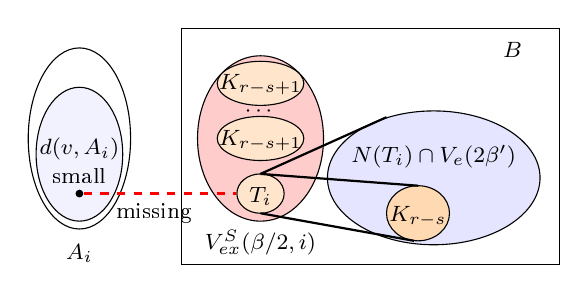
\begin{tikzpicture}[
    node distance=1.5cm,
    set/.style={ellipse, draw, minimum width=1.3cm, minimum height=2.3cm},
    smallset/.style={ellipse, draw, minimum width=1.1cm, minimum height=1.7cm},
    smallset0/.style={ellipse, draw, minimum width=1.6cm, minimum height=2.1cm},
    ssmallset/.style={ellipse, draw, minimum width=2.7cm, minimum height=1.7cm},
    sssmallset/.style={ellipse, draw, minimum width=1.1cm, minimum height=0.56cm},
    ssssmallset/.style={ellipse, draw, minimum width=0.6cm, minimum height=0.5cm},
    sssssmallset/.style={ellipse, draw, minimum width=0.8cm, minimum height=0.7cm},
    label/.style={above, font=\footnotesize},
    point/.style={circle, fill=black, inner sep=1pt},
    box/.style={draw, rectangle, minimum width=4.8cm, minimum height=3cm},
]

% 绘制 A_i 集合 (r-2个)


\node[set, fill=blue!0] (A3) at (5.2,0) {};
\node[smallset, fill=blue!5] (A4) at (5.2,-0.2) {};
\node[label] at (5.2,-0.4) {$d(v,A_i)$};
\node[label] at (5.2,-0.7) {small};
\node[label] at (5.2,-1.7) {$A_i$};
\node[point] (v) at (5.2,-0.7) {};

\node[smallset0, fill=red!20] at (7.5,0) (B) {};
\node[label] at (7.5,-1.6) {$V_{ex}^S(\beta/2,i)$};

\node[sssmallset, fill=orange!20] at (7.5,0.7) (C1) {};
\node[label] at (7.5,0.43) {$K_{r-s+1}$};
\node[sssmallset, fill=orange!20] at (7.5,0) (C2) {};
\node[label] at (7.5,0.15) {$\cdots$};
\node[label] at (7.5,-0.28) {$K_{r-s+1}$};

\node[ssssmallset, fill=orange!20] at (7.5,-0.7) (C3) {};
\node[label] at (7.5,-0.98) {$T_i$};
\draw[thick,dashed,red] (v)--(C3);
\node[label] at (6.15,-1.2) {missing};

\node[ssmallset, fill=blue!10] (A4) at (9.7,-0.5) {};
\node[box] at (8.9,-0.1) {};
\node[sssssmallset, fill=orange!30] at (9.5,-0.95) (C4) {};
\node[label] at (9.5,-1.25) {$K_{r-s}$};
\node[label] at (10.7,0.9) {$B$};
\draw[thick] (7.5,-0.45)--(9.1,0.27);
\draw[thick] (7.5,-0.95)--(9.45,-1.3);
\draw[thick] (7.5,-0.45)--(9.5,-0.60);
\node[label] at (9.7,-0.5) {$N(T_i)\cap V_{e}(2\beta')$};
\end{tikzpicture}
    \caption{Process of covering  $V_{ex}^S(\beta/2,i)$.}
    \label{fig:cover-S}
\end{figure}

By Claim \ref{degree-V-S}, one has 
$d(u,B)\ge |B|- \beta n/2- 2\alpha^{1/4}n$ for each $u\in T_i$. 
Thus, 
\begin{align}\label{common-T}
|N(T_i,B)|\ge|B|-t_i \cdot \frac{\beta n}{2}-t_i\cdot 2\alpha^{1/4}n\ge |B|-r\cdot \beta n.
\end{align}
By Definition \ref{Partition} \ref{B3}, we get that $|B\cap V_e(2\beta')|\ge |B|-r\sqrt{\alpha} n.$ %Let $X_i\subseteq  B\cap V_{e}(2\beta')$ be the set of vertices belonging to some $K_{r-s+1}\in \mathcal{F}_k$ with $k<i$. Notice that each $\mathcal{F}_k$ with $k<i$ is constructed in the same manner as above, i.e., each copy of $K_{r-s+1}$ in $\mathcal{F}_k$  is either entirely contained in $V_{ex}(\beta/2,i)$, or contains at most $r-s-1$ vertices in $B\cap V_e(2\beta')$. This establishes the bound $|X_i|\le (i-1)(r-s)$. 
%The construction of Notice that each $\{\mathcal{F}_k\}_{k<i}$ establishes the bound $|X_i|\le (i-1)(r-s)$. 
Then 
$$
|B_{T_i}|\ge |B|-r\beta n-r\sqrt{\alpha}n-\sum_{k<i}\Big\lceil \frac{s_k}{r-s+1}\Big\rceil\cdot (r-s+1) \ge |B|-(r+1)\beta n.%\ \text{and}\ d(v,B) \ge (1-\frac{1}{r-s})|B|-1\ \text{for every}\ v\in B_{T_i}\setminus S.
$$ 
It follows from Ore's condition that  $\sigma(G[B])\geq 2\big(1-\frac{1}{r-s}\big)|B|-2.$
Thus,
\begin{align*}
    \sigma(G[B_{T_i}])&\geq \sigma(G[B])-2(r+1)\beta n\geq 2\Big(1-\frac{1}{r-s}\Big)|B|-(2r+3)\beta n\\
    &\geq 2\Big(1-\frac{1}{r-s-1}\Big)|B_{T_i}|.
\end{align*}
%$$\sigma(G[B_{T_i})])\ge 2|B|-(2r+3)\beta n$$
%then 
%$$\sigma(G[B_{T_i})])\ge 2(1-\frac{1}{r-s-1}-3r\beta)|G[B_{T_i})]|$$.
%Consider $G[B_{T_i}]$, we obtain $d_{G[B_{T_i}]}(v)\ge d(v,B\setminus S)-(r+1)\beta n$. Since $|B|=\frac{r-s}{r}n$ and $\beta\ll \frac{1}{r}$, we have 
%$$d_{G[B_{T_i}]}(v)\ge(1-\frac{1}{r-s})|B|-1-(r+1)\beta n\ge  (1-\frac{1}{r-s-1})\big|G[B_{T_i}]\big|.$$ 
Note that $G[B_{T_i}]$ contains no $\frac{\gamma_{s+1}^2}{4}$-independent set of size $\frac{n}{r}$, and hence no $\frac{\gamma_{s+1}^2}{10}$-independent set of size $\frac{|B_{T_i}|}{r-s}$. By Proposition \ref{SuperT}, we conclude that $G[B_{T_i}]$ contains $K_{r-s}$ as a subgraph. By selecting $r-s+1-t_i$ vertices from this $K_{r-s}$ and combining them with $T_i$, we obtain a $K_{r-s+1}$ that covers $T_i$.  Together with the existing $\lfloor s_i/(r-s+1)\rfloor$ copies, it  forms the desired family $\mathcal{F}_i$.
\end{proof}
%Taking $r-s+1-t_i$ vertices from this $K_{r-s}$ and combining with $T_i$ gives a $K_{r-s+1}$ covering the remaining $t_i$ vertices in $V_{ex}^S(\beta/2,i)$, which together with the $\lfloor s_i/(r-s+1)\rfloor$ existing copies forms $\mathcal{F}_i$.%Select $r-s+1-t_i$ vertices from such a $K_{r-s}$ and combine them with $T_i$ to form a $K_{r-s+1}$ covering the remaining $t_i$ vertices in $V_{ex}^S(\beta/2,i)$. This $K_{r-s+1}$ together with the $\left\lfloor s_i/(r-s+1)\right\rfloor$ copies of $K_{r-s+1}$ selected earlier forms the desired $\mathcal{F}_i$.

% In the following, we prove the second part of this claim. 


% (i) %If $s_i=1$, then assume that 
% Recall that $u$ is the unique vertex in $V_{ex}^S(\beta/2,i)$.  %By the above argument, we obtain that $d(u)\ge (1-\frac{1}{r})n-2\alpha^{1/4}n.$ Thus, 
% It follows from \eqref{degree-ex-S} that  $d(u, B\setminus S)\ge |B\setminus S|-\beta n.$ Let $B_u:=\big (N(u,B\setminus S) \cap V_e(2\beta')\big )\setminus X_i$. Then by Fact \ref{SizeofS} one has 
% $$
% |B_u|\ge |B\setminus S|-\beta n-r\sqrt{\alpha}n-(i-1)(r-s)\geq \frac{n}{r}-2\beta n.
% $$ 
% Based on  Definition \ref{Partition} \ref{B2} and the condition that $e(G[B\setminus S, S])<\eta n^2$,  we conclude that $G[B_u]$ contains at least one edge. Combining the vertex $u$ with any such edge in $G[B_u]$ yields the required $K_3$ subgraph. %there exists an edge in $G[B_u]$. The vertex $u$ combined with the edge in $G[B_u]$ forms the desired $K_3$.

% (ii) Let $V'$ be an arbitrary subset of $V_{e}^S(2\beta')$ with $|V'|\le 2$. Obviously,  $G[V_{ex}^S(\beta/2,i)\cup V']$ is a clique. Hence, one may get a family of vertex-disjoint $K_3$ copies covering the vertices in $V'$ and all but at most two vertices in $V_{ex}^S(\beta/{2}, i)$. For the remaining uncovered vertices, a similar argument to (i) demonstrates the existence of the required $K_3$ subgraph to cover them. 
%For those uncovered vertices, by employing a similar argument as (i), we know that there is a desired $K_3$ to cover them.  % and First, we find a $K_3$ covered $x$. Next, we greedily find $K_3$ in the remaining vertices of $G[V_{ex}^S(\beta, i)]$; at most two vertices remain uncovered by these $K_3$. 
%For these uncovered vertices, following the process similar to (i), we construct a $K_3$ that covers the vertices by using vertices in $(B\setminus S)\cap V_e(2\beta').$ Thus, we obtain a $\mathcal{F}_i$ of size $|\mathcal{F}_i|= \left\lceil (s_i+1)/3\right\rceil$.




Let $\mathcal{F}_i$ be the family obtained in Claim \ref{r-scover} for each $i\in [s]$. % and let $\mathcal{F}_i=\emptyset$ otherwise. 
%It follows from \eqref{degree-ex-S} that $V_{ex}^S(\beta/2,i)\cap V_{ex}^S(\beta/2,j)=\emptyset$ for any $i\neq j$. % every vertex $v\in V_{ex}^S(\beta/2,i)$ does not in $V_{ex}^S(\beta/2,j)$ for any $j\neq i$. 
For all distinct $i,j\in [s]$ and each $K_{r-s+1}\in \mathcal{F}_i$, since  $V(\mathcal{F}_i)\subseteq \left(B\cap V_{e}(2\beta')\right)\cup V_{ex}^S(\beta/2,i)$,  together with Claim \ref{degree-V-S} we have 
\begin{align}\label{base-F}
    |N(V(K_{r-s+1}),A_j)|\ge |A_j|-(r-s+1)\cdot \max \bigg\{\frac{\beta}{2}n+2\alpha^{1/4}n, 2\beta' n\bigg \} \ge (1-r^2\beta)\frac{n}{r}.
\end{align}
%Thus, let $D_0=A_i$ and $D_1=B$, each $K_{r-s+1}\in \mathcal{F}_i$ satisfies \ref{C03} and \ref{C04} with $\xi=\beta/4$ and $C_1=K_{r-s+1}$. % when $K_{r-s+1}=C_1$, $A_i=D_0$, and $B=D_1$.  

Next, we are to construct the second component of each base in $\mathcal{F}^S$. 
\begin{claim}\label{com-2}
    For each $i\in [s]$ with $s_i>0$, there exists a family $\mathcal{F}_i'$ of vertex-disjoint subgraphs satisfying
    \begin{itemize}
        \item $|\mathcal{F}_i'|=f(s_i,r-s)$;
        \item $|V(F') \cap A_i|=2$ for each $F'\in \mathcal{F}_i'$;
        \item for any pair  $F\in \mathcal{F}_i$ and 
        $F'\in \mathcal{F}_i'$, their union $F\cup F'$ forms a $(2,\beta/4)$-base in $G$. 
    \end{itemize}
    %subgraphs $F'$ with $|\mathcal{F}_i'|=|\mathcal{F}_i|$, where each $F'$ satisfies \ref{C03} and  \ref{C04}  with $\xi=\beta /4$. Moreover, $|V(F') \cap A_i|=2$ for each $F'\in \mathcal{F}_i'$.
\end{claim}

\begin{proof}[Proof of Claim \ref{com-2}]
%We first construct a larger family $\mathcal{F}_i''$. 
Fix an $i\in [s]$ with $s_i>0$,  suppose the desired $\mathcal{F}_k'$ have been constructed for all $k < i$. We split our proof into the following two cases. % For each $i\in [s]$, $\mathcal{F}_i'$ is constructed via the same method. Without loss of generality, let us consider $V_{ex}^S(\beta/2, i)$ for some $i\in [s]$. We split our proof into the following two cases.

%\medskip
%\textbf{Case 1. } $V_{{ex}}^L(\beta/2, i) = \emptyset$. %There are no $(\beta/2,i)$-exceptional vertices in $G-S$.
%\medskip

%In this case, the proof follows by distinguishing cases according to the size of $V_{b}(2\beta,i)$.

\medskip
\textbf{Case 1.} $|V_b(2\beta,i)|\ge f(s_i,r-s)$.
\medskip

In this case, we construct $\mathcal{F}_i'$ by utilizing vertices in  $V_{b}(2\beta,i)$. Observe that $V_{b}(2\beta, i)$ contains the following two types of vertices:
\begin{enumerate}[label =\rm  {\bf Type \arabic{enumi}}, leftmargin=6em]
    \item\label{v1} Vertices that are $(\beta/2,j)$-exceptional for some $j\in [s]\setminus \{i\}$;
    \item\label{v2} Vertices that are not $(\beta/2,j)$-exceptional for any $j\in[s].$ 
\end{enumerate}


%Vertices in $V_{b}(2\beta, i)$ fall into two types: $\rm(1)$ those that are $(\beta/2,i)$-exceptional for some $j\ne i$; $\rm (2)$ those that are not $(\beta/2,i)$-exceptional for any $j\in[s].$ 

Let $x$ be a vertex in $V_{b}(2\beta,i)$ that is of \ref{v1}, that is,  $x\in V_{ex}(\beta/2,j)$ for some $j\in [s]\setminus \{i\}$. By Definition \ref{Partition} \ref{B4}, there exists an edge $xy\in E(M_j)$ with $y\in A_j$ and  $d(x,A_j),d(y,A_j)\le 2\beta n$. Together with $x,y\notin S$, we obtain $d(\{x,y\},D)\ge |D|-4\beta n-2$ for each $D\in \mathcal{Q}\setminus \{A_j\}$. Recall that \eqref{size-of-ne} implies that at most  $4r\alpha^{1/4}n$ vertices have been used in all previously constructed bases, including those in $\mathcal{F}_k'$ with $k<s$. %$|V(\bigcup_{k=1}^s\mathcal{F}_k)|\le 2r\alpha^{1/4}n.$ 
%$|V_{ex}(\beta/2)|\le |V_{ne}(2\beta')|\leq 2\alpha^{1/4}n$ and $|V_b(2\beta, i)|\le \sqrt{\alpha} n.$, that is, 
Together with $|V_b(2\beta, i)|\le \sqrt{\alpha} n$, there are at least
$$d(\{x,y\},A_i)-\big|V_{ne}(2\beta')\cup %V\big(\bigcup_{k=1}^s\mathcal{F}_k\big)\cup 
V_b(2\beta,i)\big|-4r\alpha^{1/4}n\ge \frac{n}{r}-5\beta n$$
vertices in $\big(V_{e}(2\beta')\setminus V_b(2\beta,i)\big)\cap N(\{x,y\},  A_i)$ that remain unused by any previous base. % $\bigcup_{k=1}^s\mathcal{F}_k$. 
Choose $z$ to be one such vertex. % possible choices for the vertex $z$, as desired. % vertices $z$ such that $G[\{x,y,z\}]$ is the desired component. 
%We claim that there exists a vertex $z\in V_{e}(2\beta')\cap N(\{x,y\},  A_i)$ and $z$ is not in other previous bases. If so, t
Then for any $D\in \mathcal{Q}\setminus \{A_i, A_j,B\}$ we have  
$$d(\{x,y,z\},D) \ge |D|-4\beta n-2-2\beta'n\ge |D|-5\beta n,\ \text{and}\ d(\{x,y,z\},B) \ge |B|-4\beta n-2-\big(\frac{n}{r}+1\big).$$
Together with \eqref{base-F}, the union of $G[\{x,y,z\}]$ and any $F\in \mathcal{F}_i$ satisfy \ref{C03}-\ref{C04}, and thus forms a $(2,\beta/4)$-base in $G$.

Next, suppose $x\in V_{b}(2\beta,i)$ is of \ref{v2}. Then, $d(x,A_j)\ge \beta n/2$ for all $j\in [s]$ and $d(x,B)\ge |B|-n/r-1$. Since $|V_{ne}(2\beta')|\le 2\alpha^{1/4} n$ by \eqref{size-of-ne}, there are at least
$$d(x,A_i)-\big|V_{ne}(2\beta')\cup %V\big(\bigcup_{1=1}^s\mathcal{F}_i\big)\cup 
V_b(2\beta,i)\big|-4\alpha^{1/4} n\ge \frac{\beta n}{3}$$
vertices in $\big(V_{e}(2\beta')\setminus V_b(2\beta,i)\big)\cap N(x,  A_i)$ that are not used in any previous bases. %$\bigcup_{k=1}^s\mathcal{F}_k$. 
Choose $z$ to be one such vertex. % possible choices, as desired.
%We claim that  there exists a vertex $z\in N(x,A_i)\cap V_{e}(2\beta')$ and $z$ is not covered by any other previous bases. If so, t
Then for any $D\in \mathcal{Q}\setminus \{A_i,B\}$ we have 
$$d(\{x,z\},D)\ge d(x,D)-\big(|D|-d(z,D)\big)\ge \frac{\beta n}{2}-2\beta'n\ge\frac{\beta n}{3},\ \text{and}\ d(\{x,z\},B)\geq |B|-\frac{n}{r}-3\beta'n.$$
%and similarly
%$$
%d(\{x,z\},B)\geq |B|-\frac{n}{r}-3\beta'n.
%$$
Combining with \eqref{base-F}, the union of $G[\{x,z\}]$ and any $F\in \mathcal{F}_i$ satisfy \ref{C03}-\ref{C04}, and thus forms a $(2,\beta/4)$-base in $G$. %Therefore, \ref{C04} holds with $\xi=\beta /4.$ Meanwhile, the condition \ref{C03} holds with $xz$ being the desired base. 

As $\alpha\ll \beta$, we can construct a family  $\mathcal{F}_i'$ of $f(s_i,r-s)$ vertex-disjoint subgraphs such that for every $F'\in \mathcal{F}_i'$ and every  $F\in\mathcal{F}_i$, the  union $F\cup F'$ forms a $(2,\beta/4)$-base in $G$.  %By using vertices in $V_{b}(2\beta,i)$, one may  select $\big\lceil \frac{s_i+2}{r-s+1} \big\rceil$ vertices and construct corresponding vertex-disjoint subgraphs $H$ satisfying \ref{C03} and \ref{C04} with $\xi=\beta n/4$, whose union forms $\mathcal{F}_i''$.
%Select $\left\lceil (s_i+1)/(r-s+1)\right\rceil$ vertices in $V_{b}(2\beta,i)$, we obtain $\left\lceil (s_i+1)/(r-s+1)\right\rceil$ vertex-disjoint subgraph $H$ satisfying \ref{C03} and \ref{C04} with $\xi =\beta n/4$. Combine those subgraphs forms the desired $\mathcal{F}_i'.$ 


\medskip
\textbf{Case 2.} $|V_b(2\beta,i)|< f(s_i,r-s)$.
\medskip

We claim that $G[A_i\setminus (V_b(2\beta,i)\cup V(M_i))]$ contains a matching $M^*_i$ of size $f(s_i,r-s)-|V_{b}(2\beta,i)|$. %, where for each edge in $M_i^*$, both endpoints do not lie in $V_b(2\beta,i)$. 
If so,  then for any $uv\in E(M_i^*)$ and $D\in \mathcal{Q}\setminus\{A_i\}$ we have $d(\{u,v\}, D)\ge |D|-4\beta n-2$. Therefore, \eqref{base-F} implies that the union of any edge in $M_i^*$ and any $F\in \mathcal{F}_i$ satisfy \ref{C03}-\ref{C04}, and thus forms a $(2,\beta/4)$-base in $G$. In the following, we will prove the existence of  $M_i^*$.

%that is, the condition \ref{C04} holds with $\xi=\beta /4$. Meanwhile, \ref{C03} holds obviously with $uv$ being the desired base. %clear holds for $uv$. 
 

%Consider the number of vertices
%Let $v$ be a vertex in  $A_i$ with $d(v, V_{ex}^S(\beta/2,i))< b_is_i$, where 

%Let $b_i=1/9$. 
Notice that $e(G[V_{ex}(\beta/2,i), A_i])\le \frac{\beta}{2}n \cdot |V_{ex}(\beta/2,i)|.$ 
Therefore, %there are at most 
$$\Big|\big\{v\in A_i:d(v, V_{ex}(\beta/2,i))\ge \frac{1}{9}|V_{ex}(\beta/2,i)|\big\}\Big|\leq \frac{|V_{ex}(\beta/2,i)|\beta n}{2}\cdot{\frac{1}{\frac{1}{9}|V_{ex}(\beta/2,i)|}}\le 5 \beta n.$$ 
%If $uv\in M_i$, then \ref{B4} implies that $d(u,A_i),d(v,A_i)\le 2\beta n$. Thus, we obtain that 
Furthermore, by \ref{B4} one has 
$$
\Big|\{v\in A_i:d(v, V(M_i)\cap A_i) \ge \frac{8}{9}|E(M_i)|\}\Big|\leq \frac{e(G[V(M_i)\cap A_i, A_i])}{\frac{8}{9}|E(M_i)|}\leq \frac{2\beta n|E(M_i)|} {\frac{8}{9}|E(M_i)|}\le 4\beta n.
$$
%$$\frac{s_i\beta n/r}{ b_is_i}\le \frac{n}{2r}$$ vertices $v\in A_i$ satisfying $d(v, V_{ex}^S(\beta/2,i))\ge b_is_i-1$. 
Hence, there exists a set $A_i'\subseteq A_i\setminus (V_b(2\beta, i)\cup V(M_i)\cup N(V_{ex}^S(\beta/2,i)))$ of size at least $\frac{n}{2r}$ such that each vertex $v\in A_i'$ satisfying  
$$
d(v, V_{ex}(\beta/2,i))<\frac{|V_{ex}(\beta/2,i)|}{9},\ \text{and}\ 
d(v, V(M_i)\cap A_i)<\frac{8}{9}|E(M_i)|.
$$ %every vertex $v\in A_i'$ is not $(2\beta, i)$-bad and 
%$d(v, V_{ex}^S(\beta/2,i))<\frac{s_i}{9}$ for each $v\in A_i'$. 
Choose $v\in A_i'$. Since $v\notin N(V_{ex}^S(\beta/2,i))$, i.e., there exists a vertex $u\in S$ such that $uv\notin E(G)$, Ore's condition implies that 
$d(v)\ge (1-\frac{1}{r})n$. 
Thus, 
 \begin{align*}
     d(v, A_i)\geq \Big(1-\frac{1}{r}\Big)n-\big|V(G)\setminus (A_i\cup V_{ex}({\beta}/2,i))\big|-d(v,V_{ex}({\beta}/2,i))\ge \Big \lceil \frac{8 |V_{ex}(\beta/2,i)|}{9}\Big \rceil.
 \end{align*}
% \begin{align*}
%     d(v, A_i)&\geq d(v)-|(\underset{D\ne A_i}{\cup}D)\setminus V_{ex}(2\beta,i)|-d(v,V_{ex}({\beta}/2,i))\ge \left \lceil \frac{8 |V_{ex}(\beta/2,i)|}{9}\right \rceil.
% \end{align*}
%Combining the above argument, we obtain that
Therefore, 
\begin{align*}
    d\big(v, A_i \setminus (V_b(2\beta, i)\cup V(M_i))\big)&\ge \big(d(v, A_i)-d(v,V(M_i))\big)-|V_b(2\beta,i)|\geq \Big \lceil \frac{8 s_i}{9}\Big \rceil-|V_b(2\beta,i)|\\
    &\ge f(s_i,r-s)-|V_{b}(2\beta,i)|.
\end{align*}
Together with $|A_i'|\gg 2s_i$, there exists a matching $M_i^*$ of size $f(s_i,r-s)-|V_{b}(2\beta, i)|$ inside $G[A_i',A_i \setminus (V_b(2\beta, i)\cup V(M_i))]$. %Since there are no $(\beta/2, i)$-exceptional vertices in $A_i$, 


Note that all other existing bases can be chosen to be vertex-disjoint from all $M_i^*$.  Together with the argument in Case~1, there exists a family of $|V_b(2\beta, i)|$ vertex-disjoint subgraphs that covers $V_b(2\beta, i)$. Combining those with $M^*$ gives a family $\mathcal{F}_i'$ of size $f(s_i,r-s)$ such that for any $F'\in \mathcal{F}_i'$ and   $F\in\mathcal{F}_i$, the union $F\cup F'$ forms a $(2,\beta/4)$-base in $G$.
\end{proof}



By the above argument, we have 
$\left \lceil s_i/(r-s+1)\right\rceil =|\mathcal{F}_i|\le |\mathcal{F}_i'|=f(s_i,r-s).$ Notice that when $s_i\ge 2$ and $r-s\ge 2$, it holds that $|\mathcal{F}_i'|=|\mathcal{F}_i|+1$. Let $\mathcal{F}_i''$ be a subfamily of $\mathcal{F}_i'$ with size exactly $|\mathcal{F}_i|$. 
Thus, by combining  $\mathcal{F}_i$ and $\mathcal{F}_i''$, we obtain a  $\beta/4$-base set $\mathcal{F}_i^S$ of size $\left \lceil s_i/(r-s+1)\right\rceil$. %Moreover, when $s_i\ge 2$ and $r-s\ge 2$, there exists subgraph in $\mathcal{F}_i'$ which are not used by $\mathcal{F}_i^S$. 
Define $\mathcal{F}^S:=\bigcup_{i\in [s]}\mathcal{F}^S_i$. Clearly,  $\mathcal{F}^S$ is a $(2, \beta/4)$-base set that covers  $V_{ex}^S(\beta/2)$. % Moreover, every vertex of $V_{ex}^S(\beta/2,i)$ lies in some component of $\mathcal{F}_i$ for every $i\in [s]$.  Define $\mathcal{H}_2:=\bigcup_{i\in [s]}\mathcal{F}_i\cup \mathcal{F}_i'$. It is routine to check that $\mathcal{H}_2$ is a $(2, \beta/4)$-base set such that every vertex of $V_{ex}^S(\beta/2)$ belongs to some component of  $\mathcal{H}_2$. %.  can be formed by combining elements of $\mathcal{F}_i$ and $\mathcal{F}_i'$ such that every $v\in V_{ex}^S(\beta/2)$ lies in some component of  $\mathcal{H}_2$. 

Let $\mathcal{F}^L_*$ be a maximal subset of $\mathcal{F}^L$ where every graph is vertex-disjoint from all graphs in $\mathcal{F}^S$.  
Hence, $\mathcal{F}:=\mathcal{F}^L_*\cup \mathcal{F}^S$ is the desired $\beta/4$-base set. 
\end{proof}

Lemma \ref{Exceptional} guarantees the existence of a $\beta/4$-base set $\mathcal{F}$ covering $V_{ex}(\beta/2)$. However, vertices in $V_{ne}(2\beta')\setminus V_{ex}(\beta/2)$ may still fail to satisfy the conditions of Lemma~\ref{GHH2024}. We  %there may exist vertices in  $V(G) \setminus V_{ex}(\beta/2)$ that 
%fail to satisfy the condition of Theorem \ref{KM}. Next, we 
next construct a base set covering $V_{ne}(2\beta')\setminus V_{ex}(\beta/2)$. %, namely those for which $d(v,D) < (1-\frac{1}{r})|D|$ holds for some $D \in \mathcal{Q}$. To address this, we construct an additional base set  $\mathcal{L}$ with the property that every non-excellent vertex (i.e., every vertex in $V_{\text{ne}}(2\beta')$) is contained in some $L \in \mathcal{L}$.
%However, there may remain vertices $v\in V(G)\setminus V_{ex}(\beta/2)$ such that $d(v,D)< (1-\frac{1}{r})|D|$ for some $D \in \mathcal{Q}$, and these vertices do not satisfy the condition of Theorem \ref{KM}. Thus, let us construct another family $\mathcal{L}$ such that every non-excellent vertex lies in some $L\in \mathcal{L}$. Here, non-excellent vertices refer to those in $V_{ne}(2\beta')$.

%Based on the above argument, we have found a set of bases that covers all $(\beta/2, i)$-exceptional vertices. The following aiming is that let us find a $(2, \beta/3)$-base or a $(1,\beta/3)$-base covering each vertex $v\in V_{ne}$ but $v\not \in V_{ex}(\beta/2,i)$ for all $i$. Let $\mathcal{H}_{ex}$ denote the set of bases covered $(\beta/2,i)$-exceptional vertices, we have $|V(\mathcal{H}_{ex})|\le \alpha^{1/3} n$. Then we have the following three claims.

\begin{lemma}\label{Vne}
Suppose that \ref{assumption} holds, and let  $U\subseteq V(G)$ be a vertex subset with $|U|\le 4r\alpha^{1/4} n$. %For any vertex $v\in V_{ne}(2\beta')\setminus V_{ex}(\beta/2)$, t
Then there exists a $\beta/4$-base set that covers $V_{ne}(2\beta')\setminus V_{ex}(\beta/2)$ and avoids $U$. Moreover, every vertex in this base set that does not belong to $B$ has degree at most $ (1-2\beta')n$. %, where each base is either a $(2,\beta/4)$-base or a $\beta/4$-base $L_v$ that contains a vertex $v\in V_{ne}(2\beta')\setminus V_{ex}(\beta/2)$, such that every $u\in V(L_v)\setminus B$ satisfies $d(u)\le n-2\beta' n$. % lies in some $L\in \mathcal{L}$. % and each $L \in \mathcal{L}$ is disjoint with $W$.

% {\color{orange}Moreover, if $s=r-2$, $e(G[B\setminus S,S])<\eta n^2$ and $V_{ne}^S(2\beta')\setminus V_{ex}^S(\beta/2)\neq \emptyset$, then the following hold:}
%  \begin{enumerate}
% [label =\rm  (F\arabic{enumi})]
%      \item\label{F1}  there exists a $(2,\frac{\beta}{4})$-base set $\mathcal{L}$ that covers $\big(V_{ne}(2\beta')\cup\{x\}\big)\setminus V_{ex}(\beta/2)$ for any $x\in V_e^S(2\beta')$. %, every vertex in $\big(V_{ne}(2\beta')\cup\{x\}\big)\setminus V_{ex}(\beta/2)$ is contained in some  $L\in \mathcal{L}$.
%      \item\label{F2}  $|V(L) \cap V_e^S(2\beta')|$ and $|V(L) \cap (B \setminus V_e^S(2\beta'))|$ have the same  parity for every $L\in \mathcal{L}$ except the one containing vertex the $x$.  
%      %|V(L)\cap V_e^S(2\beta')|$ and $|V(L)\cap \big(B\setminus V_{e}^S(2\beta')\big)|$ have the same parity for all $L\in \mathcal{L}$ except for the base containing the vertex $x$.
% %(F_1)和（F_2)没用到，直接删去
%  \end{enumerate}

\end{lemma}

\begin{proof}
Choose $v\in V_{ne}(2\beta')\setminus V_{ex}(\beta/2)$. If $s=r$, then $\delta(G)\geq (1-\frac{1}{r})n-1$ and one may assume $v\in A_i$ for some $i\in [r]$. Thus, $d(v,
A_j)\ge \beta n/2$ for every $j\in [n]\setminus \{i\}$. Therefore, the vertex $v$ itself is a $\beta/4$-base under the partition $\mathcal{Q}$. In what follows, we only consider the case that $s<r$. 

Recall that 
$$
v\in V_{ne}(2\beta')=V(G)\setminus V_{e}(2\beta')\ \text{and}\ V_{e}(2\beta')=\bigcap_{D\in \mathcal{Q}}(V_e(2\beta',D)\cup D).
$$
Hence there exists a set $D\in \mathcal{Q}$ such that $v\in V(G)\setminus (V_{e}(2\beta',D)\cup D)$. We split the proof into the following two cases. 

\medskip
\textbf{Case 1.} $v\notin B$. %The Vertex $v\in V(G)\setminus (V_{e}(2\beta',D)\cup D)$ for some $$ is not $(2\beta',D)$-excellent and $v\notin B.$
\medskip


Since $v\notin B$, without loss of generality, assume that $v\in A_i$ for some $i\in [s]$. Let $D$ be a set in $\mathcal{Q}$ such that $v\in V(G)\setminus (V_{e}(2\beta',D)\cup D)$. 
Since $v\notin V_e(2\beta',D)$, we obtain 
$$
d(v,A_i)\geq \Big(1-\frac{1}{r}\Big)n-1-|V(G)\setminus (A_i\cup D)|-d(v,D)\geq |D|-1-(|D|-2\beta'n)=
2\beta' n-1.
$$
%Since $v\notin V_{ex}(\beta/2)\cup  V_e(2\beta',D)\cup B$, we obtain 
%$$
%d(v,D')\geq \frac{\beta n}{2}\ \text{for every}\ D'\in \mathcal{Q}\setminus \{A_i,B\},\ %%d(v,A_i)\geq 2\beta' n-1\ 
%\text{and}\  d(v,B)\geq |B|-\frac{n}{r}-1.
%$$ 
%Furthermore, since $d(v,D)\leq |D|-2\beta'n$ one has  
%$$
%d(v,A_i)\geq \big(1-\frac{1}{r}\big)n-1-|V(G)\setminus (A\cup D)|-d(v,D)\geq 2\beta' n-1
%$$
%% $d(v,D)\ge |D|-\frac{n}{r}+\beta n/2-1$ for all $D\in \mathcal{D}$. 
As $|V_{ne}(2\beta')| \le  2\alpha^{1/4}n$ and $|U|\le 4r\alpha^{1/4} n,$ we obtain %the number of vertices in $(N(v, A_i)\cap V_e(2\beta' ))\setminus U$ that are not used in the previous bases is at least % There are at least 
$$\big|(N(v, A_i)\cap V_e(2\beta' ))\setminus U\big|=d(v,A_i)-|V_{ne}(2\beta')|-|U|\ge \beta' n.$$
%vertices $u\in N(v,A_i)$ such that every $u$ is not contained in the bases we have constructed with $v\in V_e(2\beta' )$ and $v\notin W$,  
Since $G[A_i]$ is $\sqrt
{\alpha}$-independent, there are at most $2r\sqrt{\alpha} n (\ll \beta'n)$ vertices $u\in A_i$ such that $d(u)\ge n-2\beta' n$.
Choose $w\in (N(v, A_i)\cap V_e(2\beta' ))\setminus U$ such that $d(w)\le n- 2\beta' n$. %, then the edge $uv$ is a component contained in the desired base. It is clear that the condition \ref{C03} holds. 
Since $v\notin V_{ex}(\beta/2)$ and $w\in V_e(2\beta')$, for each $D'\in \mathcal{Q}\setminus \{A_i,B\}$, we deduce  
\begin{align}\label{eq:uv-co}
    |N(\{v,w\},D')|\ge \frac{\beta n}{2}-2\beta'n\geq\frac{\beta n}{4}\ \text{and}\ |N(\{v,w\},B)|\ge |B|-\frac{n}{r}-3\beta'n.
\end{align} %|D|-\frac{n}{r}+\frac{\beta n}{2}-1-2\beta'n\ge |D|-\frac{n}{r}+\frac{\beta n}{4},
%$$
%Therefore, \ref{C04} holds  with $\xi=\beta /4$. 

%Next, we will show that $G$ contains a clique $K_t$ with $|V(K_t)\cap B|=r-s+1$ satisfying the conditions \ref{C03} and \ref{C04} with $\xi =\beta /4$.
Let $B':=B\setminus (V_{ne}(2\beta')\cup U)$. % denote the set of vertices that are not used in any previous bases. 
Then $$|B'|\ge \frac{r-s}{r}n-|V_{ne}(2\beta')|-|U|\ge \frac{r-s}{r}n-5r\alpha^{1/4} n.$$
Based on $\sigma(G)\ge2(1- \frac{1}{r})n-2$, we get 
$$\sigma(G[B'])\ge \Big(1-\frac{1}{r-s}-\alpha^{1/5}\Big)|B'|.$$
Since $G[B]$ contains  no $\gamma_{s+1}^2/4$-independent set of size $\frac{n}{r}$, Proposition \ref{SuperT} implies that there exists a copy of $K_{r-s+1}$ in $G[B']$. %Such a $K_{r-s+1}$ is the desired $K_t$. 
It is straightforward to check that such a $K_{r-s+1}$ together with the edge $vw$ satisfy \ref{C03} and \ref{C04} with $\xi =\beta /4$, and thus forms a $(2,\beta/4)$-base in $G$, as desired. % Let such a $K_{r-s+1}$ be a base. Then it is clear that \ref{C03} holds. Since every vertex in the $K_{r-s+1}$ lies in $V_e(2\beta')$, the condition \ref{C04} holds with $\xi =\beta /4$.

% {\color{orange}Next, we consider $s=r-2$ and $e(G[B\setminus S,S])<\eta n^2$. %, we construct the other component with more detailed information.
% If $|S|\le \frac{n}{r}-\beta n$, then 
% $d(v,B\setminus S) \ge \frac{\beta n}{2}$. Therefore,
% $$
% d(v,(B\setminus (S\cup W)) \cap V_{e}(2\beta'))\geq \frac{\beta n}{3}.
% $$
% %That is, there exists at least $\beta n/4$ vertices in $\big (B\setminus (S\cup W)\big) \cap V_{e}(2\beta')$ that not used in the previous bases. 
% Let $B'\subseteq  (B\setminus (S\cup W)) \cap V_{e}(2\beta')$ be a vertex set containing the vertices not used in the previous bases. Then $|B'|
% \ge \frac{n}{r}$. By Proposition~\ref{SuperT}, there exists a copy of $K_3$ in $G[B']$. Combining such a $K_3$ with edge ${uv}$ forms a $(2,\beta/4)$-base. 

% Now, we assume that $|S|>\frac{n}{r}-\beta n$. If $d(v,B\setminus S)\ge \frac{n}{2r}$, then $B'\subseteq N(v,B\setminus S)\cap (V_e(2\beta')\setminus W)$ to be a vertex set containing the vertices not used in the previous bases. Hence $|B'|\ge \frac{n}{2r}-\beta n$. Since $e(G[B\setminus S, S])<\eta n^2$, we have $e(G[B'])> \frac{|B'|^2}{4}$. Therefore, $G[B']$ contains a copy of $K_3$. Combining such a $K_3$ with the edge ${uv}$ forms a $(2,\beta/4)$-base. If $d(v,B\setminus S)< \frac{n}{2r}$, then $d(v,S)\ge \frac{n}{2r}-1$. Since $|V_{ne}(2\beta')|\le \alpha^{1/4}n$, there exists a vertex set $B''\subseteq V_e^S(2\beta')$ of size at least $\frac{n}{r}-2\beta n$ %vertices in $S$ that lies in $V_e^S(2\beta')$
% that avoids vertices in the previous bases. Consider three distinct and arbitrarily chosen vertices in $B''$. Since $G[S]$ is a clique, these vertices form a $K_3$. Combining this $K_3$ with the edge $uv$ yields a $(2,\beta/4)$-base.}

%Consider three arbitrary different vertices in $B''$, these vertices forms a $K_3$ as $G[S]$ is a clique. Combining such a $K_3$ with edge ${uv}$ forms a $(2,\beta/4)$-base.

% \medskip
% \textbf{ Case 2.} $v\in V(G)\setminus (V_e(2\beta',i)\cup A_i)$ for some $i\in [s]$ and $v\notin B$.
% \medskip%the vertex $v$ is not $(2\beta',i)$-excellent and $v\in V(G)\setminus (A_i\cup B)$.

% By an argument analogous to Case 1, there exists an edge $uv \in E(G[A_j])$ and a $K_{r-s+1}\subseteq G[B]$ such that their union forms the desired $(2,\beta/4)$-base.

% %By employing a similar argument as Case 1, one may %The proof of case $2$ is similar to case $1$. Assume $v\in A_j$. Let us 
% %obtain an edge $uv \in E(G[A_j])$ and a $K_{r-s+1}\subseteq G[B]$, whose union  forms %. The edge $uv$ combined with the $K_{r-s+1}$ forms 
% %the desired $(2,\beta/4)$-base.

\medskip
\textbf{ Case 2.} $v\in B$. % Vertex $v$ is not $(2\beta',A_i)$-excellent for some $A_i$ and $v\in B$
\medskip %the vertex $v$ is not $(2\beta',i)$-excellent and $v\in B$.

%In this case, we will find  a $K_{r-s}$ containing the vertex $v$ such that $V(K_{r-s})\setminus \{v\}\subseteq B\cap V_e(2\beta')$. % such that $V(K_{})$ every $x\in V(K_{r-s})$ except $v$ lies in $V_e(2\beta')$. 
%By applying the same argument as above, it is routine to check that such a $K_{r-s}$ is a $(1,\beta/4)$-base under the partition $\mathcal{Q}$.

In this case, there exists an $i\in [s]$ such that  $v\in V(G)\setminus (V_{e}(2\beta',A_i)\cup A_i)$. It follows from Claim \ref{degree-V-S} that % Let $R_v:=A_i\setminus N(v)$. Since $v\notin V_e(2\beta',A_i)$, we have $|R_v|\ge 2\beta' n$. As $A_i$ is a $\sqrt{\alpha}$-independent set, there exists a vertex $u\in R_v$ such that $d(u)\le (1-\frac{1}{r})n +\alpha^{1/4} n$. Recall that $\sigma(G)\ge 2(1-\frac{1}{r})n-2$. Then $d(v)\ge (1-\frac{1}{r})n-2\alpha^{1/4}n$, which implies 
$$d(v,B)\ge \frac{r-s-1}{r}n+2(\beta'-\alpha^{1/4})n.$$ 
Let $B':= N(v, B)\setminus (V_{ne}(2\beta')\cup U)$. It is straightforward to check that $|B'|>\frac{r-s-1}{r}n$ and $\sigma(G[B'])\ge 2(1-\frac{1}{r-s-1})|B'|-2$. Recall that $G[B]$ contains  no $\gamma_{s+1}^2/4$-independent set of size $\frac{n}{r}$. 
Thus, Proposition \ref{SuperT} implies that $G[B']$ contains a copy of $K_{r-s-1}$. Therefore, there exists a copy of $K_{r-s}$ containing $v$, which forms a $\beta/4$-base under  the partition $\mathcal{Q}$, as desired. % we obtain the desired $K_{r-s}$.

\medskip
As $\alpha\ll \beta'$ and $|V_{ne}(2\beta')|\leq 2\alpha^{1/4}n$, by applying the above argument iteratively, we deduce that for each vertex $v\in V_{ne}(2\beta')$, there is a base covering $v$ that avoids all vertices used in any previously constructed bases.
\end{proof}%for each vertex $v\in V_{ne}(2\beta')$, by applying the argument as above, one may find a base to cover each $v$ avoiding all vertices used in all previous bases. \
% If $r-s=2$ and $e(G[B\setminus S,S])<\eta n^2$, then %every vertex $v\in V_{ne}(2\beta')$ satisfies that 
% together with Fact \ref{SizeofS} one has $d(v,B\setminus S)\ge \beta n$. Therefore, there exists a vertex $u\in N(v,B\setminus S)\cap\big(V_e(2\beta')\setminus W\big)$ that is not used in the previous bases. Thus, edge $uv$ forms a $\beta/4$-base. Moreover, if $v\in V_{ne}^S(2\beta')\setminus V_{ex}^S(\beta/2)\ne \emptyset$, then %let $v$ be a vertex in $V_{ne}^S(2\beta')\setminus V_{ex}^S(\beta/2)$. C
% choose $x\in V_e^S(2\beta')$. Clearly,  $vx\in E(G)$, that is, $vx$ forms a $(1,\beta/4)$-base.

% We iteratively construct the base sets for each vertex $v \in V_{ne}(2\beta')$, thereby obtaining the desired $(2,\beta/4)$-base set.
%For each vertex $v \in V_{ne}(2\beta')$, we construct the bases one by one, yielding the desired $(2,\beta/4)$-base set.

% Let $\mathcal{P}=\{A_1,\ldots,A_s,B\}$. For $x\in V_{ne}$, if there exists $i$ such that $x$ is $(\beta/2, i)$-exceptional, there exists a vertex-disjoint base set covering $x$ by Lemma \ref{Exceptional}. Then let us cover the vertex $x$ is not $(\beta/2, i)$-exceptional for each $i$. Assume that we have cover $k$ vertices in $V_{ne}$ and each vertex covered a base with at most $r-s+3$ vertices, where $|\overset{s}{\underset{i=1}{\cup}}(X_i\cup V_{ex}^S(\beta/2, 
% i))|\le k<|V_{ne}|$, let us cover the $k+1$ vertices. Since $x\in V_{ne}$ and not $(\beta/2, i)$-exceptional for each $i$, we have that $d(x,A_i)\ge \frac{\beta}{2}$. 

% If $x\in A_i$ and $x$ is not $(\beta/2, B)$-excellent. Let $W$ be the set of vertices that are covered by some base or the vertices in $V_{ne}$, then we have $|W|\le \alpha^{1/5}n$. Since $d(x, A_i)\ge \frac{\beta}{2}n$, there are at least $\frac{\beta}{2}n-|W|\ge \frac{\beta}{4}n\gg r\sqrt{\alpha}n$ vertices. Thus, there exist a vertex $y$ such that $xy\in E(G)$ and $y$ is $(\beta', D)$-excellent for each $D\in \mathcal{H}$ and $D\ne A_i$. Let $B'$ denote the set of vertices $x\in B\setminus W$ that are $\{2\beta',j\}$-excellent for each $1\le j\le s$. Then $|B'|\ge |B|-r\sqrt{\alpha}n-\alpha^{1/5}n.$ \eqref{Ore} implies that 
% $$\sigma(G[B'])\ge 2(1-\frac{1}{r-s}-\alpha^{1/6})n.$$ And there is not $\gamma_{s+1}/4$-independent set of size $\frac{n}{r}$ in $B$. By proposition \ref{SuperT}, we get a $K_{r-s+1}$ copy in $B'$. Let $H:=K_{r-s+1}\cup\{xy\}$, then $H$ is a $(2, \frac{\beta}{4})$-base cover $x$.

% If $x\in A_i$ and $x$ is not $(\beta/2,j)$-excellent vertices for some $j\ne i$. The proof is identical to the above case.

% If $x\in B$ and $x$ is not $(\beta/2,i)$-excellent. Since $\sigma(G)\ge 2(1-\frac{1}{r-s})n-2$. then we can find a $K_{r-s}\subseteq G[B]$ such that $K_{r-s}$ cover the vertex $x$. Then, this $K_{r-s}$ is a $(1,\frac{\beta}{4})$-base.

% If $e(G[V_{\beta/4}^s,B\setminus S])\le \eta n^2$, we have that $|B|=\frac{2n}{r}$ and there are at most $\eta^{1/2}n$ vertex in $B\setminus S$ such that  vertices $d(x, B\setminus S)< |B\setminus S|-\eta^{1/2}n$. Let $K_2:=xy \in E(G[A_i])$. We have $d(K_2, B)\ge \frac{n}{2r}$. By pigeonhole principle, we have that $d(x, V_{\beta/4}^s)\ge \frac{\beta}{8}n$ or $d(x, B\setminus S)\ge \frac{\beta}{8}n$. If $d(x, V_{\beta/4}^s)\ge \frac{\beta}{8}n$, let us pick a copy of $K_3$ disjoint with $V_{ne}$ and the bases covering $V_{ne}$. If $d(x, B\setminus S)\ge \frac{\beta}{8}n$, let $B''$ denote the set of vertices such that $d(x, B\setminus S)\ge |B\setminus S|-\eta^{1/2}n$. We can find a $K_3\subseteq B\setminus S$ and $K_3$ is disjoint with $V_{ne}$ and the bases covering $V_{ne}$, that is, $(2,\beta/4)$-base $H$ covering vertex $x$ is balanced.


\subsection{Proof of Lemma \ref{K_r-tiling}}\label{section7.2}

In this subsection, we will give the proof of Lemma \ref{K_r-tiling}. First, we show that the bases constructed above can be extended to some vertex-disjoint $K_r$ and the rest partition still has some good properties. 
% By Lemma \ref{Exceptional} and Lemma \ref{Vne}, we can obtain a $\beta/4$-base set $\mathcal{H}$ covering all vertices in $V_{ne}(\beta/2)$. We can classify the bases $H\in \mathcal{H}$ into the following types. 
% \begin{enumerate}
%     \item[{\rm (i)}] $V(H)\cap \big (V_{ne}(2\beta')\setminus V_{ex}(\beta/2)\big )\neq \emptyset$ and $V(H)\cap V_{ex}^S(\beta/2)=\emptyset;$
%     \item[{\rm (ii)}] $V(H)\cap V_{ex}^L(\beta/2)\ne \emptyset$ and $V(H)\cap \big (V_{ne}(2\beta')\setminus V_{ex}^L(\beta/2)\big )=\emptyset;$
%     \item[{\rm (iii)}] $V(H)\cap V_{ex}^S(\beta/2)\ne \emptyset$ and $V(H)\cap \big (V_{ne}(2\beta')\setminus V_{ex}(\beta/2)\big )=\emptyset.$
% \end{enumerate}

\begin{lemma}\label{extend}
Suppose that \ref{assumption} holds. Let $H$ be a $\beta/5$-base or $(2,\beta/5)$-base in $G$, and $W$ be a vertex subset satisfying $|W| \leq 5r\alpha^{1/4}n$. Then, there exists a $K_r$-tiling ${T}_H$ in $G-W$ that covers $V(H)$, consisting of at most two vertex-disjoint cliques and  satisfying 
%Let $H\in \mathcal{H}$ and $W$ be a vertex subset satisfying $|W| \leq 4r\alpha^{1/4}n$. For each $H\in \mathcal{H}$, 
%Then, there exist at most two vertex-disjoint $K_r$ copies in $G-W$ that cover $V(H)$. %, and these cliques are vertex-disjoint across different $H$. 
%Denote by $T_H$ the vertex set of the cliques covering $H$. Then for every $D \in \mathcal{Q}$, we have 
\[
|T_H \cap V(D)| = \frac{kr|D|}{n}\ \text{for every}\ D\in \mathcal{Q}.
\]
\end{lemma}
\begin{proof}%[Proof of Lemma~\ref{extend}]

We first consider a $\beta/5$-base $H\in \mathcal{H}$. Let $t_H:=r-s-|V(H)\cap B|$. By \ref{C02} one has $|N(V(H),B)|\ge (t_H-1)\frac{n}{r}+\frac{\beta n}{5}$. Let $G':=G[(N(V(H), B)\setminus W)\cap V_{e}(2\beta')]$. Clearly, 
$$|V(G')|\ge (t_H-1)\frac{n}{r}+\frac{\beta n}{5}-5r\alpha^{1/4} n-2\alpha^{1/4} n\ge (t_h-1)\frac{n}{r}+\frac{\beta n}{8}.$$ 
Since $\sigma(G)\ge 2(1-\frac{1}{r})n-2$, one has 
$$\sigma(G')\ge 2|V(G')|-\frac{2n}{r}-2\ge 2\Big(1-\frac{1}{t_H-1}\Big)|V(G')|.$$
By \ref{B2}, $G'$ contains no $\frac{\gamma_{s+1}^2}{4}$-independent set of size $\frac{n}{r}$. %If $t_h\ge 2$, then 
Proposition \ref{SuperT} implies that there exists a $K_{t_H}$ in $G'$. Define  $H'$ as the join of this $K_{t_H}$ and $H$. Since $H$ is a $\beta/4$-base, for every $A_i\in\mathcal{Q}$ with $|A_i\cap V(H)|=0$ we have
$$|(N(H',A_i)\setminus W)\cap V_e(2\beta')|\ge \frac{\beta n}{5}-r \cdot 2\beta' n-5r\alpha^{1/4} n-2\alpha^{1/4} n\ge \frac{\beta n}{8}.$$
This enables us to iteratively select vertices $x_i\in \big(N(H',A_i)\cap V_e(2\beta')\big)\setminus W$ for each $i\in [s]$ with $|A_i\cap V(H)|=0$. Therefore, $G[V(H')\cup \{x_i:|A_i\cap V(H)|=0\ \text{and}\ i\in [s]\}]$ is a clique $K_r$, as desired. % $H'':=H'+x$ is still a clique in $G$. 
%That is, there exists a $K_r$ with $V(K_r)\subseteq V(G)\setminus W$ covering $H$.

Next, we assume that $H$ is a $(2,\beta/5)$-base in $\mathcal{H}$. %Based on \ref{C04}, w
Without loss of generality, assume that $C_0$ and $C_1$ are two vertex-disjoint cliques in $H$ and $D_0, D_1 \in \mathcal{Q}$ are two parts satisfying $|N(C_i)\cap D_i|=\frac{r|D_i|}{n}+1$. % \ref{C03} and \ref{C04}. 
For $C_0$, we will find a vertex set $T_1\subseteq D_1\setminus W$ of size $t_1:=\frac{r|D_1|}{n}-|V(C_0)\cap D_1|-1$ such that $G[V(C_0)\cup T_1]$ is a clique. % $C_0':=C_0\vee T_1$ is a subgraph of $G$. 
If $t_1\le0$, then it is trivial. Thus, we only need to consider $D_1=B$ and $r-s\ge 2$. Let $G':=G[(N(C_0,B)\cap V_{e}^S(2\beta'))\setminus W]$. %Then by \ref{C04} one has 
%$$|V(G')|\ge |B|-(r-s-t_1+1)\frac{n}{r}+\frac{\beta n}{5}-8r\alpha^{1/4} n-2\alpha^{1/4} n\ge (t_1-1)\frac{n}{r}%\left(1-\frac{2}{r-s}\right)|B|
%+\frac{\beta n}{8}.$$
%Since $\sigma(G)\ge 2(1-\frac{1}{r})n-2$, we obtain 
%$$\sigma (G')\ge 2|V(G')|-\frac{2n}{r}-2\ge 2\left(1-\frac{1}{t_1-1}\right)|V(G')|.$$
%It follows from  \ref{B2} that $G'$ contains no  $\frac{\gamma_{s+1}^2}{4}$-independent set of size $\frac{n}{r}$. Proposition \ref{SuperT} implies that there exists a $K_{t_1}$ in $G'$. Define $H'$ to be the join of this $K_{t_1}$ and $H$.  Clearly, $H'$ is a clique in $G$. 
By applying a similar argument as the case that $H$ is a $\beta/5$-base, we conclude that 
$G'$ contains $K_{t_1}$ as a subgraph and there exists a copy of $K_r$ covering $K_{t_1}\cup C_0$ that avoids $W$ and all used vertices. 

%If $t_1= 1$, then $|G'|\ge \frac{\beta n}{8}>0$. Let $H':=H+\{v\}$, where $v\in V(G')$, we have $H'\subseteq G$. 
%For each parts $D\in \mathcal{Q}\setminus \{D_0,D_1\}$, there exist $\frac{r |D|}{n}-|V(C_0)\cap D|$ vertices in $D\setminus W$ contained in $N(C_0')$ by the similar argument of $H$ is a connected graph. Thus, we get a $K_r$ covering $C_0$. 
By the same argument, there exists a copy of $K_r$ covering $C_1$ that avoids both $W$ and all previously used vertices. Moreover, the union of these two $K_r$ copies uses two distinct vertices from each $A_i\setminus W$ for each $i\in [s]$ and $2(r-s)$ vertices from $B\setminus W$, as required. 
\end{proof}

% \begin{fact}\label{SizeofS}
% {\color{blue}Suppose that \ref{assumption} holds. If $s=r-2$, then $|S|<\frac{n}{r}+\alpha^{1/4}n$.}
%     % Let $G$ be an  $n$-vertex graph with $\sigma(G)\ge 2(1-\frac{1}{r})n-2$. Assume that  $\mathcal{Q}$ is an $(r,r-2;\gamma_{r-2},\gamma_{r-1};S)$-good partition of $G$, where $S=\{v\in V(G):d(v)<(1-\frac{1}{r})n-1\}.$ 
%     %For an arbitrary graph $G_{s}$, when $r-s=2$, we have that  % number of vertices $v\in S$ is less than $\frac{n}{r}+\alpha^{1/4}n$. 
% \end{fact}
% \begin{proof}
% It follows from Definition \ref{Partition} \ref{B1} that $e(G[A_i])\le \sqrt{\alpha}n^2$ for every $i\in [r-2]$. Since $d(v)\ge (1-\frac{1}{r})n-1$ for every $v\in V(G)\setminus S$, we have
% \begin{align*}   
% e(G[A_i,S])&={\sum_{v\in A_i}}d(v,S)={\sum_{v\in A_i}}\big(d(v)-d(v,V(G)\setminus (A_i\cup S))-d(v,A_i)\big)\\
% &\ge \frac{n}{r}\cdot (|S|-1)-2\cdot e(G[A_i]).
% \end{align*}
% By calculating the sum of vertex degrees within the set $S$, we obtain 
% \begin{align*}
% \underset{v\in S}{\sum}d(v)=|S|(|S|-1)+{\sum_{i=1}^{r-2}}e(G[A_i,S])\ge \left(\frac{r-2}{r}n+|S|\right) \cdot(|S|-1)-2(r-2)\sqrt{\alpha}n^2.
% \end{align*}
% Taking the average of $|S|$, we derive
% $$\left(\frac{r-2}{r}n+|S|\right) \cdot\left(1-\frac{1}{|S|}\right)-\frac{2(r-2)\sqrt{\alpha}n^2}{|S|}\le d(S)<\left(1-\frac{1}{r}\right)n-1.$$
% Consequently, $|S|< \frac{n}{r}+\alpha^{1/4}n$, as desired.     
% \end{proof}

Now, we are ready to prove Lemma \ref{K_r-tiling}. 
\begin{proof}[\bf Proof of Lemma \ref{K_r-tiling}] 
Recall that $|V_{ne}(2\beta')|\le 2\alpha^{1/4} n$. By Lemma \ref{Exceptional} and Lemma~\ref{Vne}, we obtain a $\beta/4$-base set $\mathcal{H}$ covering $V_{ne}(2\beta')$ with at most $12\alpha^{1/4}n$ vertices. Let $W:=V(\mathcal{H})$. We then proceed iteratively: at each step, we apply Lemma~\ref{extend} to extend a base to a \( K_r \)-tiling, and then update \( W \) by adding the vertices of this new \( K_r \)-tiling. Therefore, we obtain a \( K_r \)-tiling \( \mathcal{T} \) of order at most \( 4r \alpha^{1/4} n \) that covers \( V_{\mathrm{ne}}(2\beta') \).  
%Let $W$ be the vertex set of the union of $V(\mathcal{H})$ and vertices covered by the extended $K_r$. Repeated application of Lemma~\ref{extend} allows us to extend all bases in $\mathcal{H}$ to a $K_r$-tiling $\mathcal{T}$ of order at most $4r\alpha^{1/4}n$ that covers $V_{ne}(2\beta')$. % by applying Lemma~\ref{extend} repeatedly, one may extend all bases in $\mathcal{H}$ to a $K_r$-tiling $\mathcal{T}$ with order at most $4r\alpha^{1/4}n$ that avoids $W$ and covers $V_{ne}(2\beta')$.  %By Lemma~\ref{extend}, we iteratively extend each copy of $H \in \mathcal{H}$, where $W$ is the set of all used vertices and all vertices in $\mathcal{H}$. Through this process, we obtain a $K_r$-tiling $\mathcal{T}$ with order at most $4r\alpha^{1/4}n$ that covers $V_{ne}(2\beta')$. 
Let $G':=G-V(\mathcal{T})$, $A_i':=A_i\setminus V(\mathcal{T})$ for each $i\in [s]$,  and  $B':=B\setminus V(\mathcal{T})$. % be a set consisting of all unused vertices in $B$. 
By Lemma~\ref{extend}, one has that  $\{A_1',\ldots,A_s',B'\}$ is an $(r,s)$-partition of $G'$ and $(r-s)\mid |B'|$. % and $|B'|\geq |B|-4r\alpha^{1/4}n$. 
Furthermore,  
\begin{align}\label{Ore:G'}
\sigma(G')\ge 2\Big(1- \frac{1}{r}\Big)n-8r\alpha^{1/4}n-2 \ \text{and} \ \sigma(G[B'])\ge 2\Big(1-\frac{1}{r-s}-\alpha^{1/5}\Big)|B'|.
\end{align} 
%$\sigma(G[B'])\ge \frac{r-s}{r}n-4(r-s)\alpha^{1/4} n-2$
%We split the proof into two parts: $\rm (i)$ $r-s\ne 2$; $\rm (ii)$ $r-s=2$. %First, let us consider the former simpler cases.  
%(i) Assume that $r-s\neq 2$. 
% with the following properties:
%\begin{itemize}
%    \item Every vertex $v \in V_{ne}(2\beta')$ is covered by some $K_r$ in $\mathcal{T}$;
 %   \item The tiling $\mathcal{T}$ uses at most $4r\alpha^{1/4}n$ vertices in $V(G)$.
%\end{itemize}
 %By the claim, let us extend $H\in \mathcal{K}$ one by one, where $W$ is the vertex set, which is the union of the unextended $H\in \mathcal{K}$ and the obtained $K_r$. We get a $K_r$-tiling $T$ such that every $v\in V_{ne}(2\beta')$ lies in some $K_r$ in $K_r$-tiling and this $K_r$-tiling utilize at most $4r\alpha^{1/4}n$ vertices in $V(G)$. 

% let us ensure that there exists a $K_{r-s}$-tiling in $G[B']$. 
Observe that $G[B']$ contains no $\frac{\gamma_{s+1}^2}{8}$-independent set of size $\frac{n}{r}$, and hence no $\frac{\gamma_{s+1}^2}{10}$-independent set of size $\frac{|B'|}{r-s}$. Clearly, \ref{L2} is trivial for $r-s=1$. If $r-s\geq 3$, then by Theorem \ref{non-extremal} we obtain that there exists a $K_{r-s}$-tiling in $G[B']$, i.e., \ref{L2} holds. %Thus, the $K_r$-tiling $\mathcal{T}$ satisfies \ref{L2} when $r-s\geq 3$. 
In what follows, it suffices to consider $r-s=2$. We will show that either $G$ is the extremal graph \ref{EX2}, or $G[B']$ contains a perfect matching, or by modifying some bases in $\mathcal{H}$ we can get a new $K_r$-tiling $\mathcal{T}'$ such that $G[B\setminus V(\mathcal{T}')]$ admits a perfect matching. 

If $G[B']$ contains a perfect matching, then we are done. Suppose that $G[B']$ contains no perfect matching. By Proposition \ref{PMatching}, we know that $G[B']$ consists of two odd components, say $F_0$ and $F_1$.
%If $G[B']$ is a connected graph, then Proposition \ref{PMatching} implies that  $G[B']$ admits  a perfect matching. Consequently, one may assume that $G[B']$ is disconnected. It follows from Ore's condition that $G[B']$ has exactly two components, say $F_0$ and $F_1$.

Suppose that $V_{ne}(2\beta')= \emptyset$. Then   $\mathcal{H}=\emptyset$ and $B'=B$. Without loss of generality, assume that  $|F_0|\le |F_1|$. 
%Lemma \ref{Exceptional} implies that $F_0, F_1$ are odd components. 
By Ore's condition, we conclude that 
$N(z)=V(G)\setminus (V(F_{i+1})\cup \{z\})\ \text{for each}\ z\in V(F_i)\ \text{with}\ i\in \mathbb{Z}_2.$ Hence %either $G[B]$ has a perfect matching, or $F_0, F_1$ are cliques with odd orders. Suppose that 
$F_0, F_1$ are two cliques with odd orders. % odd components. %By Ore's condition, each vertex $v\in V(F_i)$ is adjacent to all vertices in $V(G)\setminus (V(F_{i+1})\cup \{v\})$ for each $i\in \mathbb{Z}_2$. 
If $G[A_i]=\emptyset$ for all $i\in [r-2]$, then $G$ is the extremal graph described in \ref{EX2}. Suppose that there exists an edge $uv\in E(G[A_i])$ for some $i\in [r-2]$. Then there exists a vertex  $w\in V(F_0)$ such that $G[\{u,v,w\}]$ forms a $K_3$, say $K^1$. Since $F_1$ is a clique and $|F_1|\ge |B'|/2$, there exists a $K_3$, say $K^2$, in $F_1$. Since $V_{ne}(2\beta')=\emptyset$, it is easy to check that $K^1\cup K^2$ is a $(2,\beta/4)$-base in $G$. By applying Lemma~\ref{extend} with $W=\emptyset$, we obtain a $K_r$-tiling $\mathcal{T}$ of $G$ such that  $|V(F_i)\setminus V(\mathcal{T})|$ is even for every $i\in \mathbb{Z}_2$. Applying Proposition~\ref{PMatching} again yields that $G[B\setminus V(\mathcal{T})]$ contains a perfect matching, as desired. Thus, overall, it suffices to consider the case where 
$$
r-s=2,\ G[B']=F_0\cup F_1\ \text{with $|F_0|$ and $|F_1|$ both  odd} ,\ \text{and}\ V_{ne}(2\beta')\neq \emptyset.
$$

% Recall that $V_{ne}(2\beta')=\emptyset$. Then one may greedily find two vertex-disjoint copies of $K_r$, say $K^1$ and $K^2$ such that 
% \begin{align*}
% &V(K^1)\cap A_i=\{u,v\},\ |V(K^1)\cap C_0|=1,\ 
% |V(K^1)\cap C_1|=0,
% |V(K^1)\cap A_j|=1\ \text{for all}\ j\neq i;\\
% &|V(K^2)\cap A_i|=0,\ 
% |V(K^2)\cap C_0|=0,\ 
% V(K^2)\cap C_1=V(K'),\ 
% |V(K^2)\cap A_j|=1\ \text{for all}\ j\neq i.
% \end{align*}
% %Since each vertex $x\in V(G)$ with respect to partition $\mathcal{Q}$ of $G$ is $(2\beta',D)$-excellent for all $D\in \mathcal{Q}$, that is, there exists a copies of $K_r$ which occupies one vertex in $C_0$ and $A_j$ with $j\ne i$, no vertices in $C_1$, and two vertices $v,u \in A_i$. 
% % Therefore, we can extend such a $K_3$ to a $K_r$ such that it contains no vertices in $A_i$, one vertex in each $A_j$ with $j\ne i$.  
% Let $G^*:=G-V(K^1\cup K^2)$, $B^*:=B\setminus V(K^1\cup K^2)$, and $\mathcal{Q}^*$ be the partition obtained from $\mathcal{Q}$ by removing vertices in $V(K^1\cup K^2)$. %By removing those two $K_r$ copies from the graph $G$, the partition $\mathcal{Q}$ and the set $B$, we denote the remaining graph by $G'$, partition by  $\mathcal{Q}'$ and set by  $B'$, respectively.   %Let $G'$ be the subgraph of $G$ induced by removing the vertices of these two $K_r$ copies, and $\mathcal{Q}'$ be a  partition of $G'$, which is obtained from $\mathcal{Q}$ by deleting the vertices covered by these two $K_r$ copies. 
% Clearly, $\mathcal{Q}^*$ remains an $(r,s)$-partition of $G^*$ and  $G^*[B^*]$ consisting of two even components. 
% %Let $G'$ denote the induced graph of $G$ by removing these two $K_r$ copies and the partition $\mathcal{Q}$ of $G'$, derived from $Q$ by deleting the vertices in these two $K_r$, is an $(r,s)$-partition. Meanwhile, we have that $B'$ has two even components, where $B'\in \mathcal{Q}$. 
% Together with Proposition \ref{PMatching}, we know that $G^*[B^*]$ admits a perfect matching. Thus, \ref{L2} holds. 

%Suppose that $G[B']$ contains no perfect matching. Then  Proposition \ref{PMatching} implies that both $F_0$ and $F_1$ are odd components. 
Our goal is to  modify the $K_r$-tiling $\mathcal{T}$ into a new $K_{r}$-tiling $\mathcal{T}'$ that satisfies \ref{L2}. We begin with an analysis of the properties of $F_0$ and $F_1$.  %We have the following properties. 
Since $S$ is a clique in $G$, at most one of the components $F_i$ with $i\in\mathbb{Z}_2$ satisfies $V(F_i)\cap S\neq \emptyset.$  Without loss of generality, assume that $V(F_1)\cap S=\emptyset$. Therefore, for a vertex $v\in V(F_1)$, one has 
$$
\Big(1-\frac{1}{r}\Big)n-1\leq d(v)\leq n-|B'|+d(v,F_1),
$$
which implies 
$$
|F_1|\geq d(v,F_1)\geq \frac{n}{r}-1-4r\alpha^{1/4}n\geq \frac{n}{r}-\alpha^{1/5}n. 
$$
Furthermore, if $|F_1|\ge \frac{n}{r}+1$, then $d(u)\leq (1-\frac{1}{r})n-2$ for every $u\in V(F_0)$. That is,  $V(F_0)\subseteq S$.  Similarly, if $V(F_0)\setminus S\neq \emptyset$, then $|F_0|\geq \frac{n}{r}-\alpha^{1/5}n.$ In particular, if $|F_0|\leq \frac{n}{r}-3\beta n$, then by Ore's condition one has 
\begin{align}\label{complete}
G[V_{ex}^L(\beta/2)\cup (V(G)\setminus (V_b(2\beta)\cup B)),V(F_0)]\ \text{is a complete bipartite graph}.
\end{align}

% there are no perfect matchings in $G[B']$. 




%We will construct a $K_r$-tiling $\mathcal{T}'$ for each type of bases. Before proceeding with the construction, let us first specify some properties of the components $F_0$ and $F_1$. 

%We claim that $|F_1| \ge \frac{n}{r}-\alpha^{1/5}n$. If not, then $|F_0|>\frac{n}{r}$. Thus, every vertex $v\in F_1$ has at most $(1-\frac{1}{r})n-2$ neighbors in $G$, that is, $v\in S$, which contradict to $S\cap F_1=\emptyset$. If $|F_1|\ge \frac{n}{r}+1$, then $E\big(G[V(F_0),V(F_1)]\big)=\emptyset$ implies every vertex $v\in V(F_0)$ has at most $(1-\frac{1}{r})n-2$ neighbor in $G$. Fact \ref{clique} implies that $V(F_0)\subseteq S$. 

For any $\Tilde{\mathcal{H}}\subseteq \mathcal{H}$, let $\Tilde{\mathcal{T}}\subseteq \mathcal{T}$ be the set of $K_r$ copies obtained by extending the bases in $\widetilde{\mathcal{H}}$. Let $X_{\Tilde{\mathcal{H}}} :=\big(B\cap V(\Tilde{\mathcal{T}})\big)\setminus V_{ex}^S(\beta/2)$. It follows from \eqref{size-of-ne} that $|X_{\Tilde{\mathcal{H}}}|\le 8\alpha^{1/4}n$. % and $S \subseteq V(F_0)\cup \big(B\cap V(\mathcal{T})\big)$. 
If $|F_1|\ge \frac{3n}{2r}$, 
then define 
\begin{align}\label{eq:F_0}
F_0'(\Tilde{H}):=G\big[V(F_0)\cup (X_{\Tilde{\mathcal{H}}}\cap S)\big] \ \text{and} \ F_1'(\Tilde{H}):=G\big [(V(F_1)\cup X_{\Tilde{\mathcal{H}}})\setminus S\big];
\end{align}
if $|F_1|< \frac{3n}{2r}$, then define  
\begin{align}\label{eq:F_1}
F_1'(\Tilde{H}):=G\big[V(F_1)\cup \{x\in X_{\Tilde{\mathcal{H}}} : d(x,F_1)\ge \frac{2}{3}|F_1|\}\big] \ \text{and} \ F_0'(\Tilde{H}):= G\big[(V(F_0)\cup X_{\Tilde{\mathcal{H}}})\setminus V(F_1')\big].
\end{align}
For brevity, when $\widetilde{H}$ is clear from context, we write $F_0'$ and $F_1'$ for $F_0'(\widetilde{H})$ and $F_1'(\widetilde{H})$, respectively.
Note that if $V_{ex}^S(\beta/2) \cap V(\Tilde{\mathcal{H}})=\emptyset$, then 
\begin{align}\label{even-order}
|V(F_0\cup F_1)|\ \text{and}\ 
|V(F_0'\cup F_1')|\ \text{are even}.
\end{align}
The following claim demonstrates that both $F_0'$ and $F_1'$ remain connected even after the deletion of any small subset of vertices.

\begin{claim}\label{Connected}
For any $\Tilde{\mathcal{H}}\subseteq \mathcal{H}$ and any $X'\subseteq V(F_0'\cup F_1')$ of size at most $10\alpha^{1/4}n$, we have that $F_0'':=G[V(F_0')\setminus X']$ and $F_1'':=G[V(F_1')\setminus X']$ are connected.
\end{claim}
\begin{proof}[Proof of Claim \ref{Connected}]
   We first consider that $|F_1|\ge \frac{3n}{2r}$. % It suffices to check two cases, respectively. First, when $|F_1|\ge \frac{3n}{2r}$, it is clear that 
   Clearly, $F_0'$ is a clique, and thus $F_0''$ is connected. %Let us show that $G[V(F_1')\setminus X']$ is connected. 
For two vertices $x\in V(F_0)$ and $y\in V(F_1)$, we have
$$
2\Big(1-\frac{1}{r}\Big)n-2\leq d(x)+d(y)\leq 2(n-|B'|)+|F_0|-1+d(y,F_1).
$$
Thus, 
\begin{align}\label{eq:degree-y}    
d(y,F_1'')\geq d(y,F_1')-|X'|\geq d(y,F_1)-|X'|\geq |F_1|-1-|B\setminus B'|-|X'|\geq |F_1|-20\alpha^{1/4}n. 
\end{align}
    %For any $y\in V(F_1)$, we have that $d(y,B)\ge |F_1|-1$. Since $E\big(G\big[V(F_0),V(F_1)\big]\big)=\emptyset$, we have $d(y,F_1'')\ge  |V(F_1'')|-|X|-1.$ 
    For any $y'\in V(F_1')\setminus V(F_1)$, we have
    $$ 
    d(y',F_1'')\ge d(y',F_1')-|X'|\geq d(y',B)-(|F_0|+|B\setminus B'|+|X'|)\ge \frac{n}{r}-1-\big(\frac{n}{2r}+20\alpha^{1/4}\big)\geq \frac{n}{3r}.
    $$
    Therefore, for any two distinct vertices $u,v\in V(F_1'')$, we obtain $N_{F_1''}(u)\cap N_{F_1''}(v)\neq \emptyset$ unless $u,v\in V(F_1'')\setminus V(F_1)$. Consequently, $F_1''$ is connected. 
    %$d(y',B)\ge \frac{n}{r}-1$. Since $|V(F_0)\cup X|\le \frac{n}{2r}$, $d(y',F_1'')\ge d(y',B)-|V(F_0)\cup X\cup X'|\ge \frac{n}{3r}.$ Let us consider the degree sequence of $F_1''$, we have
    %$\frac{n}{3r}\le d(x_1)\le\dots \le d(x_i)\le |F_1''|-|X|-1\le d(x_{i+1})\le \dots \le d(x_{|X|+1})\le \dots \le d(x_{|F_1''|}).$$
    %Since $|X|\ll |F_1''|$, for any $i\in\big[|F_1''|\big]$, we have $d(x_i)+d(x_{|F_1''|-i})\ge |F_i''|$, that is, $F_1''$ is connected.

    Now, we assume  $|F_1|<\frac{3n}{2r}$. For any $y'\in V(F_1'')\setminus V(F_1)$, by the construction of $F_1'$ we have $d(y',F_1'')\ge \frac{2}{3}|F_1|-|X'|\geq \frac{1}{2}|F_1''|+1$. Together with \eqref{eq:degree-y} and the classical Dirac's Theorem, we conclude that % for every $y \in V(F_1\cap F_1'')$ one has $d(y,F_1'')\ge |F_1|-20\alpha^{1/4}n$.  Dirac's Theorem implies that 
    $F_1''$ is connected.
    
   We now show that  $F_0''$ is connected. %If $V(F_0'')\subseteq S$, then $F_0''$ is connected. So, we assume that $V(F_'')\setminus S\neq \emptyset$. Thus,  , 
   Similar to \eqref{eq:degree-y} we obtain   $d(y,F_0'')\ge |F_0|-20\alpha^{1/4}\geq \frac{4}{5}|F_0''|$ for any $y \in V(F_0\cap F_0'')$. Let $y'\in V(F_0'')\setminus V(F_0)$. If there is a vertex $x\in V(F_0)\setminus N_G(y')$, then by Ore's condition we have
   $$
   2\Big(1-\frac{1}{r}\Big)n-2\leq d(x)+d(y')\leq 2(n-|B'|)+|F_0|-1+\frac{2}{3}|F_1|+d(y',F_0).
   $$
   Thus,
   $$
   d(y',F_0'')\geq d(y',F_0)-|X'|\geq \frac{1}{3}|F_1|-20\alpha^{1/4}n\geq \frac{n}{4r}>\frac{1}{5}|F_0''|,
$$
the last two  inequalities hold by $|F_1|\ge \frac{n}{r}-\alpha^{1/5} n$. Therefore, for any two distinct vertices $u,v\in V(F_0'')$, we obtain $N_{F_0''}(u)\cap N_{F_0''}(v)\neq \emptyset$ unless $u,v\in V(F_0'')\setminus V(F_0)$. It follows that $F_0''$ is connected. 
   %Since $|F_1|\ge \frac{n}{r}-\alpha^{1/5} n$, for any $y'\in V(F_0'')\setminus V(F_0)$ one has $$d(y',F_0'')\ge \max \left\{\frac{2n}{r}-2-\frac{2}{3}|F_1|-|F_0|-|X\cup X'|, \frac{1}{3}|F_1|-|X\cup X'|\right\},$$
   % that is, $d(y')\ge \frac{n}{4r}$. It is clear that $\frac{1}{5}|F_0''| \le \frac{n}{4r}$ and $|X|\ll |F_0''|$. Thus, we have $d(x_i) + d(x_{|F_0''|-i})\ge |F_0''|$ for any $i\in \big[|F_0''|\big]$, that is, $F_0''$ is connected.
\end{proof}
To allow for minor modifications, we introduce a claim that modifies a given base into a desired form. 
\begin{claim}\label{Adjust}
{For any subset $\Tilde{\mathcal{H}}\subseteq \mathcal{H}$, let  $F_0'$ and $F_1'$ be given by \eqref{eq:F_0}-\eqref{eq:F_1}. Let $K$ be a clique satisfying \ref{C03} and \ref{C04} with $\xi=\beta/4$, $C_0=K$, $D_0=A_i$ for some $i\in [r-2]$,
and $D_1=B$. % For $k=2,3$, let $K \subseteq G-B$ be a {\color{red}clique of size $k$ within a $\beta/4$-base or $(2,\beta/4)$-base $H$, satisfying $|V(K)\cap A_i|=2$ for some $i\in[r-2]$.} %, and $K'\subseteq G[B]$ be a clique of size $3$ such that $K\cup K'$ forms a $(2,\beta/4)$-base in $G$. } %  satisfying \ref{C03}} 
%{\color{purple} and $K$ satisfies \ref{C03},\ref{C04} with $C_0=K$, $D_0=A_i$, $D_1=B$, and $\xi=\beta/4$.}
Suppose that $V_{ex}^S(\beta/2) \cap V(K)=\emptyset$ and $d(K,F_j')\ge \frac{n}{3r}$ for some $j\in \mathbb{Z}_2$. If $|F_0'|\ge 2$ or $d(x)\le n-2\beta'n$ for every $x\in V(K)$, then there exists a $(2,\beta/5)$-base $H'$ such that $V(K)\subseteq V(H')$, $|B\cap V(H')|=4$ and $|V(F_\ell')\setminus V(H')|$ is even for every $\ell\in \mathbb{Z}_2$. }
%Moreover, if $d(x)\le n-2\beta'n$ for every  $x\in V(K)$, {\color{red}then there exists such an $H'$ for $C_0'$ of any size.}
\end{claim}
\begin{proof}[Proof of Claim \ref{Adjust}]
We first consider $|F_0'|\geq 2$. Since $d(K,F_j')\ge \frac{n}{3r}$ for some $j\in \mathbb{Z}_2$, there exists a vertex $w\in V(F_j')\subseteq V_{e}(2\beta')$ such that $G[V(K)\cup \{w\}]$ forms a clique $K_{k+1}$. Let such a $K_{k+1}$ be $C_0$. %It is clear that $K_{k+1}$ satisfies \ref{C03},\ref{C04}. Since $V(F_0\cup F_1)\subseteq V_e(2\beta')$, it is sufficient to construct a $K_3\subseteq F_{j+q}$ with $q\equiv |F_j'|\pmod{2}$. If $|F_0|\ge \frac{n}{7r}$, then b
By Ore's condition, for each $x\in V(F_1')$ one has 
$$d(x,F_1'-w)\ge |F_1'|-|B\setminus B'|-2\ge \frac{1}{2}|F_1'|+1.$$
Thus, Mantel's Theorem implies that $F_1'-w$ contains a $K_3$. Similarly, one may  obtain that $F_0$ contains a $K_3$ if $|F_0'|\geq \frac{n}{7r}$, and $F_0'$ is a clique if $2\le |F_0'|< \frac{n}{7r}$. %Let $C_1$ be the $K_3$ in $F_{j+k}$, where $k\equiv |F_i'|\pmod{2}$. %Such a $K_3$ is the $C_1$, as desired. 
%If $2\le |F_0|< \frac{n}{7r}$, then $F_0'$ is a clique, and Mantel's Theorem implies that there exists a copy of $K_3$ in $F_1$. 
Consequently, there exists a  $K_3$ in $F_{j+\ell}'-V(K)\cup \{w\}$, where $\ell\equiv |F_j'|\pmod{2}$. Define $C_1$ to be such a $K_3$. It is easy to check that $H':=C_0\cup C_1$ satisfy \ref{C03}-\ref{C04} with $D_0:=A_i$, $D_1:=B$, and $\xi:=\beta/5$. Together with \eqref{even-order}, $H'$ is a $(2,\beta/5)$-base such that $|B\cap V(H')|=4$ and $|V(F_i')\setminus V(H')|$ is even for every $i\in \mathbb{Z}_2$.   % Such a $K_3$ is the $C_1$, as desired. 

Now, we consider  $d(x)\le n-2\beta'n$ for every $x\in V(K)$ and $|F_0'|=1$. Let $w$ be the unique vertex in $F_0'$. Then $d(w)\le (1-\frac{2}{r})n+8\alpha^{1/4}n$. Since $\beta' \gg \alpha$, Ore's condition implies that $G[V(K)\cup \{w\}]$ is a clique, say $C_0$.  Recall that $F_1'$ contains a $K_3$, say $C_1$. %Such a $K_3$ is the $C_1$, as desired.
Thus, $H':=C_0\cup C_1$ is the desired $(2,\beta/5)$-base $H'$.
\end{proof}

 %Based on  \ref{C03} and \ref{C04}, assume $|V(K)\cap A_i|=2$ for some $i\in[r-2]$, and let $D_0:=A_i$ and $D_1:=B$. 
% Since $d(V(K),F_j)\ge \frac{n}{3r}$, there exists a vertex $w\in V(F_j)\subseteq V_{e}(2\beta')$ such that $G[V(K)\cup \{w\}]$ forms a clique $K_{k+1}$. Let such a $K_{k+1}$ be $C_0$ with $D_0:=A_i$, $D_1=B$, and $\xi=\beta/5$. It is clear that $K_{k+1}$ satisfies \ref{C03},\ref{C04}. Since $V(F_0\cup F_1)\subseteq V_e(2\beta')$, it is sufficient to construct a $K_3\subseteq F_{j+q}$ with $q\equiv |F_j'|\pmod{2}$. If $|F_0|\ge \frac{n}{7r}$, then by Ore's condition, for each $x\in F_{\ell}$ with ${\ell}\in \mathbb{Z}_2$  one has 
%$$d(x,F_{\ell})\ge |F_{\ell}|-|B\setminus B'|-1\ge \frac{1}{2}|F_{\ell}|+1.$$ 
%for every $j\in \mathbb{Z}_2$ and every $x\in F_j$. 
%Thus, Mantel's Theorem implies that both $F_0$ and $F_1$ contain a $K_3$. %Let $C_1$ be the $K_3$ in $F_{j+k}$, where $k\equiv |F_i'|\pmod{2}$. %Such a $K_3$ is the $C_1$, as desired. 
%If $2\le |F_0|< \frac{n}{7r}$, then $F_0'$ is a clique, and Mantel's Theorem implies that there exists a copy of $K_3$ in $F_1$. Thus, there exists a vertex-disjoint $K_3$ in $F_{i+k}'$, where $k\equiv |F_i'|\pmod{2}$. Such a $K_3$ is the $C_1$, as desired. 

%When $d(x)\le n-2\beta'n$ for every $x\in V(K)$, we only need to prove the case $|F_0'|=1$. Assume $w$ is the only vertex in $F_0'$ and we have $d(w)\le (1-\frac{2}{r})n+8\alpha^{1/4}n-1$. Since $2\beta n'\gg 8\alpha^{1/4}$, Ore's condition implies that $G\big[V(K_k)\cup \{w\}\big]$, say $C_0$, is also a clique in $G$.  It follows from Proposition \ref{SuperT} that $F_1$ contains a $K_3$. Such a $K_3$ is the $C_1$, as desired. Thus, a $(2,\beta/5)$-base $H'$, as desired. 

%Claim \ref{Adjust} will facilitate the completion of some minor modifications.
Based on the construction of bases in Lemma \ref{Exceptional} and Lemma~\ref{Vne}, there are three possible  types for each base  $H\in \mathcal{H}$: 
${\rm (1)}\ V(H)\cap V_{ne}(2\beta')\subseteq V_{ne}(2\beta')\setminus V_{ex}(\beta/2)$ (in Lemma~\ref{Vne}); ${\rm (2)}\ V(H)\cap V_{ne}(2\beta')\subseteq V_{ex}^L(\beta/2)$ (in Claim \ref{claim-matching}); ${\rm (3)}\ V(H)\cap V_{ex}^S(\beta/2)\ne \emptyset$ (in Claims \ref{r-scover} and \ref{com-2}). We then modify $\mathcal{T}$ into a $K_r$-tiling $\mathcal{T}'$ based on the types of bases in $\mathcal{H}$. %In what follows, we construct a $K_r$-tiling $\mathcal{T}'$ for each of the three types of bases, respectively.

\medskip
\textbf{Case 1.} There exists a base $H\in \mathcal{H}$ satisfying $V(H)\cap V_{ne}(2\beta')\subseteq V_{ne}(2\beta')\setminus V_{ex}(\beta/2).$
\medskip

%In this case, we will modify the base $H$ to obtain $\mathcal{T}'$. % only need to reconstruct one base to gain the $\mathcal{T}'$. 
By the proof of Lemma \ref{Vne}, one has 
\begin{itemize}
    \item $V(H)\cap V_{ne}(2\beta')$ contains exactly one vertex, say $v$;
    \item if $v\notin B$, then $v\in A_i$ for some $i\in [r-2]$ and $H$ is a $(2,\beta/4)$-base. More precisely, $H$ has two components $C_0$ and $C_1$ satisfying \ref{C03}-\ref{C04}, where $C_0$ is an edge $vw$ in $G[A_i]$ with $d(w)\leq n-2\beta'n$ and $C_1$ is a $K_3$ copy in $G[B\cap V_e(2\beta')]$;
    \item if $v\in B$, then $H$ is an edge  $vw$ in $G[B]$, which forms a $\beta/4$-base.
\end{itemize} 
%$|V(H)\cap V_{ne}(2\beta')|=1$. Let $v$ be the unique vertex in $V(H)\cap V_{ne}(2\beta')$. 
Suppose that $F_0'$ and $F_1'$ are defined as in \eqref{eq:F_0} and \eqref{eq:F_1} by letting $\Tilde{\mathcal{H}}:=\{H\}$. We proceed by considering whether $v$ belongs to $B$ or not. % It suffices to consider two different types of bases: $V_{ne}(2\beta')\cap V(H)\notin B$ and $V_{ne}(2\beta')\cap V(H)\in B$.

We first assume $v\notin B$. %Then by the construction in Lemma  $H$ has two components $C_0$ and $C_1$ by Lemma \ref{Vne}. 
%Without loss of generality, let $C_0\cap V_{ex}(2\beta')\ne \emptyset.$ Thus, $C_0$ is an edge $uv$, where $u\in V_{ne}(2\beta')$, $v\in V_e(2\beta')$, and $d(v)\le n-2\beta' n$.
%By Lemma~\ref{extend},
Recall that $H$ is extended to two vertex-disjoint copies of $K_r$, denoted $K^1$ and $K^2$, in $\mathcal{T}$ by Lemma~\ref{extend}.  % Let $X_H:=V(K^1\cup K^2)$, we obtain $F_0'$ and $F_1'$. 
%It follows from  $V(H)\cap V_{ex}^S(\beta/2)=\emptyset$ that $|F_0'|$ and $|F_1'|$ have the same parity. 
By \eqref{eq:uv-co} one has $d(\{v,w\},F_j')\ge \frac{n}{3r}$ for some $j\in \mathbb{Z}_2$. Claim \ref{Adjust} implies that there exists a $(2,\beta/4)$-base $H'$ such that $\{v,w\}\subseteq V(H')$, $|V(H')\cap B|=4$ and $|V(F_\ell')\setminus V(H')|$ is even for every $\ell\in \mathbb{Z}_2.$ Applying Lemma~\ref{extend} to $H'$ with $W:=V(\mathcal{T})\setminus V(K^1\cup K^2)$, one may  extend it to two vertex-disjoint copies of $K_r$ that avoids $W$, denoted  $\Tilde{K}^1$ and $\Tilde{K}^2$. Let $\mathcal{T}':=\mathcal{T}\setminus \{K^1,K^2\}\cup \{\Tilde{K}^1,\Tilde{K}^2\}$. Clearly,  $\mathcal{T}'$ is a $K_r$-tiling covering $V_{ne}(2\beta')$.  %Let $X'=V(\Tilde{K}^1\cup \Tilde{K}^2)$, 
For each $\ell\in \mathbb{Z}_2$, Claim~\ref{Connected} ensures that $G[V(F_\ell')\setminus V(\Tilde{K}^1\cup \Tilde{K}^2)]$ is a connected graph with even order. %Furthermore, $|C_0''|$ and $|C_1''|$ are even.
Combined with Proposition~\ref{PMatching}, we know  that  $G[B\setminus V(\mathcal{T}')]$ contains a perfect matching. 

Next, assume that $v\in B$. %, $H\subseteq E(G[B])$ is a $\beta/4$-base. Without loss of generality, let $v=V(H)\cap V_{ne}(2\beta)$. 
Then, $d(v,A_i)\le |A_i|-2\beta'n$ for some $i\in [r-s]$.  %By Lemma~\ref{extend},
Recall that $H$ is extended to a copy of $K_r$, say $K$, in $\mathcal{T}$. %Assume $v\in F_j'$ for some $j\in \mathbb{Z}_2$. 
Suppose that $d(v,F_{j})=0$ for some $j\in \mathbb{Z}_2$ and let $x$ be a vertex in $F_{j}$. Then\allowdisplaybreaks
\begin{align*}
2\Big(1-\frac{1}{r}\Big)n-2&\leq d(v)+d(x)\leq 2(n-|B'|)-|A_i|+d(v,A_i)+d(v,F_{j+1})+d(x,F_{j})\\
&\leq 2n-|B'|-2-2\beta'n< 2n-|B|-2=2\Big(1-\frac{1}{r}\Big)n-2,
\end{align*}
a contradiction. 
Hence, $d(v,F_j)>0$ for each $j\in \mathbb{Z}_2$.  %we have that $d(v)\le n-|F_{j+1}|-1$, that is, we obtain that 
%\begin{align*}
%    d(v,B)&= d(v)-\sum_{\ell\in [r-2]}{d(v,A_\ell)}\ge \frac{3n}{r}-|F_{j+1}'|-1-d(v,A_i)\\
%    &\ge \frac{2n}{r}-|F_{j+1}|-1+2\beta' n > |F_j| +|V(\mathcal{T})\cap B|.
%\end{align*}
%Thus, $N(v)\cap F_j'\ne \emptyset$ and $N(v)\cap F_{j+1}'\ne \emptyset$. 
Thus, there exists a $\beta/4$-base $H'$ such that $|V(H')\cap B|=2$ and $|V(F_i')\setminus V(H')|$ is even for every $i\in \mathbb{Z}_2$. By Lemma~\ref{extend}, Claim \ref{Connected} and Proposition~\ref{PMatching}, there exists a $K_r$-tiling $\mathcal{T}'$ such that $G[B\setminus V(\mathcal{T}')]$ admits a perfect matching.

% For some $i\in [s]$ and $v\in B$. Recall that in Case 3 of Lemma~\ref{Vne}, the base that we used to cover $v$ is an edge $uv$ with $u,v\in B$. Lemma~\ref{extend} extends such an edge to a copy of $K_r$ (say $K$) such that it contains one vertex from each $A_i$ and $V(K)\cap B=\{u,v\}$. % we use a $K_r$ copy (say $K$) containing $v$ is constructed by selecting one vertex from each $A_i$ and two vertices from $B$.  %Let us recover the copy of $K_r$ containing $v$. The copy occupies one vertex in each $A_i$ and two vertices in $B$. 
% %Assume that $v\in S$. Then $V(C_0)\subseteq N(v)$. 
% Notice that $d(x)\leq (1-\frac{2}{r})n+|C_i|-1+8\alpha^{1/4}n$ for each $x\in V(C_i)$ with $i\in \{0,1\}$. We claim that $d(v,C_1)\geq \beta'n$. Suppose not, then there exists a vertex in $C_1$ that is not adjacent to $v$. Hence $d(v)\geq n-1-|C_1|-8\alpha^{1/4}n$. Together with $v\notin V_e(2\beta',i)$, one has  
% $$d(v,C_1)\geq d(v,B)-|C_0|-8\alpha^{1/4}n\geq |B|-(1+|C_0|+|C_1|+16\alpha^{1/4}n)+2\beta'n>\beta'n.
% $$ 
% Similarly, either $|C_0|\leq \beta'n$ or $d(v,C_0)\geq \beta' n$. Let $X=V(K)$, we obtain $C_0'$ and $C_1'$. Choose a vertex $u\in N(v,C_j')\cap V_e(2\beta')$ such that $uv$ forms a $\beta/4$-base, where $j\equiv |C_0'|\pmod2$.
% Using Lemma~\ref{extend} to extend this base structure into a copy of $K_r$, then together with Claim \ref{Connected} and Proposition~\ref{PMatching}, the subgraph induced on the remaining vertices of $B$ contains a perfect matching.

\medskip
\textbf{Case 2.} There exists a base $H\in \mathcal{H}$ satisfying  $V(H)\cap V_{ne}(2\beta')\subseteq V_{ex}^L(\beta/2).$
\medskip

%In this case, one may assume that there are no bases in $\mathcal{H}$ satisfying Case 1.
By the construction of Claim \ref{claim-matching} in Lemma \ref{Exceptional}, we know that $H$ is an edge $uv$ with $u\in A_i\cap V_{ex}^L(\beta/2,j)$ and $v\in A_j\cap V_e(2\beta')$ for some distinct $i,j\in [s]$, which forms a $\beta/4$-base. %Let $K$ be a copy of $K_r$ that covers $V(H)$ obtained by using Lemma~\ref{extend}. % Assume that $H$ is extended by Lemma~\ref{extend} into a copy of $K_r$, say $K$, in $\mathcal{T}$. 
Suppose that $F_0'$ and $F_1'$ are defined as in \eqref{eq:F_0}-\eqref{eq:F_1} by letting $\Tilde{\mathcal{H}}:=\{H\}$. %Let $X:=B\cap V(K)$, we obtain $F_0'$ and $F_1'$. 
%Let $v\in A_j$ be the $(\beta/2,i)$-exceptional vertex in $H$ and $u\in A_i$ is another vertex of $H$. 
It is routine to check that there exists a vertex $v'\in (A_i\cap V_e(2\beta'))\setminus (V(\mathcal{T})\cup V_b(2\beta'))$ such that $G[\{u,v,v'\}]$ forms a $K_3$. Note that $d(u),d(v),d(v')\le n-2\beta'n$ and $N(\{u,v,v'\},F_j)\ge \frac{n}{3r}$ for some $j\in \mathbb{Z}_2$. %Let $C_0:=G[\{u,v,v'\}]$, $D_0:=A_j$, and $D_1:=B$. Obviously, $d(C_0,F_j)\ge \frac{n}{3r}$ for some $j\in \mathbb{Z}_2$. Claim \ref{Adjust} implies that there exists a $(2,\beta/5)$-base $H'$ such that $|V(H')\cap B|=4$ and $|V(F_\ell')\setminus V(H')|$ is even for every $\ell\in \mathbb{Z}_2$. 
Applying Claim~\ref{Adjust}, Lemma~\ref{extend}, Claim \ref{Connected} and Proposition~\ref{PMatching} again yield a $K_r$-tiling $\mathcal{T}'$ such that $G[B\setminus V(\mathcal{T}')]$ admits a perfect matching.

% Let $u\in V(H)\cap V_{ex}^L(\beta/2)$. Thus, $H$ contains exactly one edge %has only one component, and it is an edge
% $uv$ with $u\in A_i$, $v\in A_j$, where  $i,j\in[r-2]$ and $i\ne j$. Assume that $H$ is extended by Lemma~\ref{extend} into a copy of $K_r$, say $K$, in $\mathcal{T}$. 
% Let $X=V(K)$, we obtain $C_0'$ and $C_1'$. Without loss of generality, let $u$ be a $(\beta/2,j)$-exceptional vertex in $G$ and $v\in V_e(2\beta')$. Since $u,v\notin S$,  one has $d(\{u,v\},A_i)\ge \frac{n}{r}-3\beta n$. Therefore, there exists a vertex $u'\in (A_i\cap V_{e}(2\beta'))\setminus V_b(\beta,i)$ such that $G[\{u,u',v\}]$ forms a copies of $K_3$. % with $d(u')\le(1-\frac{1}{r})n+\beta n$. , as $A_i$ is a $\sqrt{\alpha}$-independent set. 
% %Since $\{u,u',v\} \subseteq V(G)\setminus S$ and $d(x,A_k)\le 2\beta n$ for some $x\in \{u,u',v\}$ and $k\in [r-2]$, we have that
% By the choices of $u,v,u'$, we have 
% $$d(\{u,u',v\},B)\ge \frac{2n}{r}-6\beta n.$$ Moreover, by \eqref{eq:uv-co} one has $d(\{u,u',v\},C_i')\ge \frac{n}{3r}$ for some $i\in \{0,1\}$. By Claim \ref{Adjust}, there exists $(2,\beta/4)$-base $H'$ such that $|V(G)\cap V(H')|=4$ and $|C_i\setminus V(H')|$ is even for every $i\in \mathbb{Z}_2$.
% %If $|C_0'|\ge 2$, then it follows by applying the same argument as the first subcase of (i). Hence, there exists a  $(\beta/4,2)$-base $H'$ with two component $Y_1$ and $Y_2$ such that $|V(Y_1\cup Y_2)\cap B|=4$ and $|C_i'\setminus V(Y_1\cup Y_2)|$ is even for every $i\in \mathbb{Z}_2$. If $|C_0'|=1$, then assume that $w$ is the unique vertex in $C_0'$. Obviously,  $d(w)\le (1-\frac{2}{r})n+\beta n$. Thus, by the Ore condition, we know that $\{u,v,u',w\}$ induces a $K_4$ in $G$. Furthermore, there exists a vertex-disjoint $K_3$ in $C_1$. {\color{red}(use a claim? then say by a similar discussion as Claim *)} Combined this with the previously obtained $K_4$, these together form a $(2,\beta/4)$-base in $G$. %By combining these two $K_3$ and $K_4$ copies, we obtain a $(2,\beta/4)$-base $H'$ in $G$. 
% Applying Lemma~\ref{extend} to $H'$ yields two disjoint copies of $K_r$, say $\Tilde{K}^1$ and $\Tilde{K}^2$. Let $\mathcal{T}':=\mathcal{T}\setminus \{K^1,K^2\}\cup \{\Tilde{K}^1,\Tilde{K}^2\}$. It is easy to check that $\mathcal{T}'$ satisfies \ref{L2}. Furthermore, by removing vertices in $\mathcal{T}'$, the size of $|C_0'|$ is even. Together with Claim~\ref{Connected} and Proposition~\ref{PMatching}, the graph induced by vertices in $G[B\setminus V(\mathcal{T}')]$ contains a perfect matching. 


\medskip
\textbf{Case 3.} There exists a base $H\in \mathcal{H}$ satisfying   $V(H)\cap V_{ex}^S(\beta/2)\ne \emptyset.$
\medskip

In this case, one may assume that no base in  $\mathcal{H}$ satisfies Case 1 or Case 2. Thus, $V_{ne}(2\beta')=V_{ex}(\beta/2)$ and $|V_{ex}^S(\beta/2)|\geq 1$. Denote $s_i:=|V_{ex}^S(\beta/2,i)|$ for each $i\in [r-2]$. By Claims \ref{r-scover} and \ref{com-2} in  Lemma \ref{Exceptional}, there exist two families $\mathcal{F}_i$ and $\mathcal{F}_i'$ of subgraphs of $G$ for each $i\in [r-2]$ with $s_i>0$, where 
\begin{itemize}
    \item $\mathcal{F}_i$ consists of $\left\lceil s_i/3\right\rceil$ vertex-disjoint $K_3$ copies such that $V_{ex}^S(\beta/2,i) \subseteq V(\mathcal{F}_i)\subseteq \left(B\cap V_{e}(2\beta')\right)\cup V_{ex}^S(\beta/2,i)$,
    \item $\mathcal{F}_i'$ consists of $f(s_i,2)$ vertex-disjoint subgraphs each of which has exactly two vertices in $A_i$, and for any pair  $F\in \mathcal{F}_i$ and 
        $F'\in \mathcal{F}_i'$, their union $F\cup F'$ forms a $(2,\beta/4)$-base in $G$. 
\end{itemize}
Moreover, each graph $F'\in \mathcal{F}_i'$ is one of the following three types:
\begin{itemize}
    \item $F'$ is a triangle $xyz$, where $x\in V_b(2\beta,i)\cap V_{ex}^L(\beta/2,j)$, $y\in V_{e}(2\beta')\cap A_j$, $z\in \big(V_{e}(2\beta')\setminus V_b(2\beta,i)\big)\cap N(\{x,y\},  A_i)$;
    \item $F'$ is an edge $xz$, where $x\in V_b(2\beta,i)\setminus V_{ex}^L(\beta/2)$ and $z\in \big(V_{e}(2\beta')\setminus V_b(2\beta,i)\big)\cap N(x,  A_i)$;
    \item $F'$ is an edge in a matching of $G[A_i\setminus (V_b(2\beta,i)\cup V(M_i))]$. 
\end{itemize}
Let $\mathcal{F}_i=\mathcal{F}_i'=\emptyset$ for each  $i\in [r-2]$ with $s_i=0$. 
%For each $i\in [s]$, let $\mathcal{F}_i$ and $\mathcal{F}_i'$ be families of graphs defined in Claim \ref{r-scover} and Claim  \ref{com-2} respectively. 
Define $F_0'$ and $F_1'$ as in \eqref{eq:F_0} and \eqref{eq:F_1} with $\Tilde{\mathcal{H}} := \mathcal{H}$. % Suppose that $F_0'$ and $F_1'$ are defined as in \eqref{eq:F_0} and \eqref{eq:F_1} by letting $\Tilde{\mathcal{H}}:=\mathcal{H}$.
Clearly, $V(F_0'\cup F_1')\subseteq V_e(2\beta')$. %, but there exists a base $H\in \mathcal{H}$ satisfying (iii). 
%In what follows, we analyze the specific structure of the base set $\mathcal{H}$. Let $X:=V(\mathcal{T})\setminus V_{ex}^S(\beta/2)$ and we obtain $F_0'$ and $F_1'$. 

Assume that there is an edge $uv\in E(G[V(F_0'),V(F_1')])$. By the construction of $\mathcal{F}_i$ in Claim~\ref{r-scover}, one may avoid $u,v$ in $\bigcup_{i\in [r-2]}\mathcal{F}_i$. Based on Lemma~\ref{extend} with $\{u,v\}\subseteq W$, there exists a $K_r$-tiling $\mathcal{T}'$ that covers all bases in $\mathcal{H}$ and  avoids $\{u,v\}$. By Claim \ref{Connected}, the graph  $F_j'':=G[V(F_j')\setminus V(\mathcal{T}')]$ is connected for each $j\in \mathbb{Z}_2$. As $uv\in E(G[V(F_0''),V(F_1'')])$, the graph  $G[V(F_0''\cup F_1'')]$ is connected. Hence, Proposition~\ref{PMatching} guarantees the existence of a perfect matching in $G[V(F_0''\cup F_1'')]$. Thus, in what follows, it suffices to consider 
\begin{align*}%\label{F0F1'}
E(G[V(F_0'),V(F_1')])=\emptyset.  
\end{align*}




 We first assume that there exists an integer $k\in[r-2]$ such that $s_k\ge 3$. Thus, $|\mathcal{F}_k'|\ge |\mathcal{F}_k|+1$. Choose $Q\in \mathcal{F}_k'$. Then $|V(Q)\cap A_k|=2$. Observe that $\mathcal{T}$ can be constructed with  $V(Q)\cap V(\mathcal{T})=\emptyset$. %that is, there exists a subgraph, say $Q\in \mathcal{F}_k'$, such that $|V(Q)\cap A_k|=2$ and $V(Q)\cap V(\mathcal{T})=\emptyset$.  
 %containing two vertices in $A_i$  $uv\in G[A_i\setminus V(\mathcal{T})]$. 
% %If $|F_0|\ge 2$, then Claim \ref{Adjust} and Lemma~\ref{extend} imply that there exists a $(2,\beta/4)$-base $H'$ such that $F_i''$ of even size is connected for every $i\in \mathbb{Z}_2$. 
Assume that $|F_0|=1$, and let $w$ be the unique vertex in $F_0$. Clearly, $w\in S$.  % is the only vertex in $F_0'$, then t
 Note that there exists a $(2, \beta/4)$-base $H:=H_1\cup H_2\in \mathcal{H}$ with $|V(H_1)\cap V_{ex}^S(\beta/2,k)|=3$ and $|V(H_2)\cap A_i|=2$. Assume that $H$ is extended to two copies of $K_r$ by Lemma \ref{extend}, denoted $K^1$ and $K^2$, in $\mathcal{T}$ with $H_2\subseteq K^2$. Let $\{x,y,z\}\subseteq V(H)$ be the three vertices in $V(H_1)\cap V_{ex}^S(\beta/2,k)$. In fact, one may assume that $|V(K^2)\cap V(F_1')|=1$. Otherwise, by replacing the vertex in $V(K^2)\cap V(F_0')$ with a vertex in $N(H_2,F_1)\cap V_e(2\beta')$, we get a new tiling $\mathcal{T}'$ such that $G[B\setminus V(\mathcal{T}')]$ contains a perfect matching. %Since $\{w,x,y,z\}\subseteq S$,  we obtain  that $G[\{x,y,w\}]\cup H_2$ satisfying $\ref{C03}$ and \ref{C04}, i.e., it forms a $(2,\beta/4)$-base. 
 Since $z\in V_{ex}^S(\beta/2,i)$, Claim \ref{degree-V-S} implies that there exist $z_1,z_2\in V(F_1')$ such that $G[\{z,z_1,z_2\}]$ is a $K_3$. %, which together with $Q$ forms a $(2,\beta/4)$-base in $G$. 
 Thus, there exist two vertex-disjoint $(2,\beta/4)$-bases $H':=G[\{w,x,y\}]\cup H_2$ and $H'':=G[\{z,z_1,z_2\}]\cup Q$ in $G$. By applying Lemma~\ref{extend}, Claim~\ref{Connected} and Proposition~\ref{PMatching}, we obtain a $K_r$-tiling $\mathcal{T}'$ covering $V_{ex}(\beta/2)$ such that $G[B\setminus V(\mathcal{T}')]$ admits a perfect matching. For the case $|F_0|\geq 2$, reapplying these results together with Claim~\ref{Adjust} yields a $K_r$-tiling $\mathcal{T}'$ with the same property.%by utilizing Claim \ref{Adjust}, and applying Lemma~\ref{extend}, Claim~\ref{Connected} Proposition~\ref{PMatching} again, we can get  a $K_r$-tiling $\mathcal{T}'$ covering $V_{ex}(\beta/2)$ such that $G[B\setminus V(\mathcal{T}')]$ admits a perfect matching. %, such that  $F_0'\setminus(H'\cup H'')=\emptyset$ and $$. 
% %Thus, there exists a perfect matching in $G[V(F_0''\cup F_1'')]$ by Claim \ref{Connected} and Proposition \ref{PMatching}. 

 Next, we assume that there exists an integer $k\in[r-2]$ such that $|V_{ex}^S(\beta/2,k)|=2$. Let $\{u,v\}=V_{ex}^S(\beta/2,k)$. It follows from \eqref{common-T} that $N(\{u,v\},F_i')\ne \emptyset$ for each $i\in \mathbb{Z}_2$. Hence, there exists a vertex $w\in V(F_j')$ for some $j\in \mathbb{Z}_2$ satisfying the following:
 \begin{itemize}
     \item $H:=G[\{u,v,w\}]\cup F'$ forms a $(2,\beta/4)$-base, where $F'\in \mathcal{F}_k'$.
     \item Assume $K^1\cup K^2$ are two vertex-disjoint $K_r$ copies covering $H$ and avoiding $V(\mathcal{T})$ (via Lemma~\ref{extend}). Define $\mathcal{T}'$ as the $K_r$-tiling obtained from $\mathcal{T}\cup \{K^1, K^2\}$ by deleting the $K_r$ copies that covered the base containing $\{u,v\}$ in $\mathcal{T}$. Then $|V(F_\ell')\setminus V(\mathcal{T})|$ is even for each $\ell\in \mathbb{Z}_2$. 
 \end{itemize}  %Then there exists a $(2,\beta/4)$-base $H'$ such that $V(H')\Delta V(H)=\{x,y\}$ with $x\in F_i'$ and $y\in F_{i+1}'$, that is, there exists $H'$ such that $F_i'\setminus H'$ is even for any $i\in \mathbb{Z}_2$. 
 Together with  Claim \ref{Connected}, and Proposition \ref{PMatching}, there exists a perfect matching in $G[B\setminus V(\mathcal{T}')]$. 
%By lemma \ref{Exceptional}, when $V_{ex}^S(\beta/2,k)\ge 2$, we have $|\mathcal{F}_k'|\ge|\mathcal{F}_k|+1.$ 
Thus, in what follows, we consider that  
\begin{align}\label{VexS}
    |V_{ex}^S(\beta/2,k)|\le 1 \ \text{for each}\ k\in[r-2].
\end{align}
%For every $i\in [r-2]$, let $\mathcal{F}_i$ and $\mathcal{F}_i'$ be family obtained in Claims \ref{r-scover} and \ref{com-2}, here $\mathcal{F}_i=\mathcal{F}_i'=\emptyset$ if $s_i=0$.  

Suppose that there exists a subgraph $L\in \bigcup_{k\in [r-2]}\mathcal{F}_k'$ such that $N(L,F_i')\neq \emptyset$ for all $i\in \mathbb{Z}_2$. 
{By an argument similar to the case that $|V_{ex}^S(\beta/2,k)|=2$ for some $k\in [s]$}, we conclude that there exists a $K_r$-tiling $\mathcal{T}'$ covering $V_{ex}(\beta/2)$ for which $G[B\setminus V(\mathcal{T}')]$ contains a perfect matching. 
%For every $L\in \cup_{k\in [r-2]}\mathcal{F}_k'$, let $L\subseteq H\in \mathcal{H}$. If $v_i\in N(L)\cap F_i'$ for any $i\in \mathbb{Z}_2$, then let $W=\{u,v\}$ and extend base set $\mathcal{H}\setminus\{H\}$, Lemma~\ref{extend} implies that $K_r$-tiling $\mathcal{T}''$. It is clear that there exists $v_i$ such that $(H\setminus L)\cup G[V(L)\cup \{v_i\}]$ is a $(2, \beta/4)$-base and $|F_i''\setminus \{v_i\}|$ is even for any $i\in \mathbb{Z}_2$. Thus, Lemma~\ref{extend}, Claim \ref{Connected}, and Proposition \ref{PMatching} implies that there exists a perfect matching in $G[V(F_0''\cup F_1'')\setminus\{v_i\}]$. 
In the following,  assume that 
\begin{align}\label{LF_k}
\text{for any}\ L\in \bigcup_{k\in[r-2]}\mathcal{F}_k', \ \text{we have}\ %i \ \text{such that} \ 
    N(L,F_i')=\emptyset \ \text{for some} \ i\in \mathbb{Z}_2.
\end{align}

Fix a $k\in [s]$ with $s_k=1$,  let $u_kv_k\in E(G[A_k])\setminus E(G[A_k\cap V_b(2\beta,k)])$. 
Since $V_{ne}(2\beta')=V_{ex}(\beta/2)$, one has $A_k\setminus V_b(2\beta,k)\subseteq V_e(2\beta')$. Without loss of generality, assume that $u_k\in V_e(2\beta')\setminus V_b(2\beta)$. Suppose that $v_k\notin V_b(2\beta,k)$. Then  $N(\{u_k,v_k\},B)\geq \frac{2n}{r}-4\beta n$ and $u_kv_k$ forms a $\beta/4$-base in $G$. It follows from \eqref{LF_k} that   $|F_0|\leq 5\beta n$. However, \eqref{complete} implies that $G[\{u_k,v_k\},V(F_0)]$ is a complete bipartite  graph, which also contradicts \eqref{LF_k}. Thus, $v_k\in V_b(2\beta,k)$. Similarly, we can show that $v_k\notin V_{ex}^L(\beta/2)$, that is,  $v_k\in V_b(2\beta,k)\setminus V_{ex}^L(\beta/2)$. Therefore, each graph in $\mathcal{F}_k'$ is exactly an edge. Moreover, $$
E(G[A_k])\setminus E(G[A_k\cap V_b(2\beta,k)])=E(G[V_e(2\beta')\setminus V_b(2\beta,k),V_b(2\beta,k)\setminus V_{ex}^L(\beta/2)]).
$$




%be an edge in some graph  $L\in \mathcal{F}_k'$ with $u_k\in V_e(2\beta')\setminus V_b(2\beta,k)$. Suppose that $v_k\notin V_b(2\beta)$ or $v_k\in V_{ex}^L(\beta/2)$. Then  $N(L,B)\geq \frac{2n}{r}-4\beta n$ and hence $N(L,F_1')\neq \emptyset$. %If $|F_0|>5\beta n$, then $N(L,F_0')\neq \emptyset$, which contradicts \eqref{LF_k}. 
%It follows from \eqref{LF_k} that   $|F_0|\leq 5\beta n$. However, \eqref{complete} implies that $G[V(L),V(F_0)]$ is a complete bipartite  graph, which also contradicts \eqref{LF_k}.  %Therefore, every vertex in $F_0'$ has degree at most  $(1-\frac{2}{r})n+3\beta n$. By Ore's condition, we have $V(F_0')\subseteq N(u)\cap N(v)$.  Together with the Ore condition there exists an $L\in \cup_{k\in[r-2]}\mathcal{F}_k'$ such that $N(L,F_i')\ne \emptyset$ for each  $i\in \mathbb{Z}_2$, contradicting assumption \eqref{LF_k}. 
%Thus, for each edge $u_kv_k\in \mathcal{F}_k'$, we must have 
%Thus, $v_k\in V_b(2\beta,k)\setminus V_{ex}^L(\beta/2)$. We further claim that every edge in $G[A_k]$ has one endpoint in $V_e(2\beta')\setminus V_b(2\beta,k)$  and the other in $V_b(2\beta,k)\setminus V_{ex}^L(\beta/2)$. Suppose that $xy\in E(G[A_k])$ with  $x\in V_b(2\beta,k)$. Then there exists a vertex  $z\in N(x,A_k)\cap (V_e(2\beta')\setminus V_b(2\beta,k))$. Together with the discussion as above, we obtain that $x\in V_b(2\beta,k)\setminus V_{ex}^L(\beta/2)$. % $G[A_k]=\emptyset$ if $V_b(2\beta,k)\setminus V_{ex}^L(\beta/2)=\emptyset$. 

%For every $x\in A_k\setminus\{v\}$, since $d(x)\ge (1-\frac{1}{r})n-1$, {\color{blue}we have $d(x,B)\ge \frac{2n}{r}-2$}. If $v\notin V_b(2\beta)$ or $v\in V_{ex}^L(\beta/2)$, then there exists an $L\in \cup_{k\in[r-2]}\mathcal{F}_k'$ such that $N(L,F_i')\ne \emptyset$ for each  $i\in \mathbb{Z}_2$, contradicting assumption \eqref{LF_k}. Thus, for each edge $u_kv_k\in \mathcal{F}_k'$, we must have $u_k\in V_b(2\beta,k)\setminus V_{ex}^L(\beta/2)$.  

Next, we show that $E(G[A_k])\setminus E(G[A_k\cap V_b(2\beta)])$ contains no edge that is vertex-disjoint from $u_kv_k$. Assume for contradiction that it contains two independent edges, say $u_kv_k$ and $u'v'$. 
%Notice that one may replace the subgraph in $\mathcal{F}_k '$ with a corresponding structure $L'$ containing $u'v'$. Hence, we can 
Assume that $u'\in V_e(2\beta')\setminus V_b(2\beta,k)$ and  $v'\in V_b(2\beta,k)\setminus V_{ex}^L(\beta/2)$.  %Without loss of generality, assume that $u'\in V_e(2\beta')\setminus V_b(2\beta,k)$ and  $v'\in V_b(2\beta,k)\setminus V_{ex}^L(\beta/2)$. 
%If $|F_0|=1$ and $u,v\notin V_{b}(2\beta,k)$, then by Ore's condition, one has $N(V(L'),F_i')\neq \emptyset$ for each $i\in \mathbb{Z}_2$, which contradicts \eqref{LF_k}. %Hence, one may assume, without loss of generality, that $u'\in V_e(2\beta')\setminus V_b(2\beta,k)$ and  $v'\in V_b(2\beta,k)\setminus V_{ex}^L(\beta/2)$.  
If $|F_0|\geq 2$, then applying Claim~\ref{Adjust} with $K=u'v'$, one may obtain a $(2,\beta/5)$-base $H'$ such that $\{u,v\}\subseteq V(H')$, $|B\cap V(H')|=4$ and $|V(F_i)\setminus V(H')|$ is even for every $i\in \mathbb{Z}_2$. %Using Lemma \ref{extend} to extend $H'$ into two $K_r$ copies, together with $\mathcal{T}$, we get the new $K_r$-tiling $\mathcal{T'}$ such that $|V(F_i)\setminus V(\mathcal{T}')|$ is even for every $i\in \mathbb{Z}_2$. 
Thus,  Lemma \ref{extend} and Proposition~\ref{PMatching} guarantee the existence of a new $K_r$-tiling $\mathcal{T}'$ such that $G[B\setminus V(\mathcal{T}')]$ has a  perfect matching. 
{Now, we assume $|F_0|=1$ and let $w$ be the unique vertex in $F_0$. Let $M^*:=\big(\bigcup_{j\in[r-2]}\mathcal{F}_j'\big)\cup \{u'v'\}$. Clearly,  $M^*$ is a matching of size $|V_{ex}^S(\beta/2)|+1$. %Let $\Tilde{\mathcal{H}}=\mathcal{H}$. Consider the components $F_0'$ and $F_1'$. 
Since $E(G[V(F_0'),V(F_1')])=\emptyset$, every vertex $u\in V(F_1')$ satisfies $d(u)\le n-|F_0'|-1$. %Let $v$ be the unique vertex in $|F_0|$ and 
By Ore's condition, one has 
$$d(w)\ge n-|F_1'|-|V_{ex}^S(\beta/2)|-1.$$
Therefore, there exists  an edge $xy\in E(M^*)$ such that $\{x,y\}\subseteq N(w)$.  %For any edge $e$ in $F$, one of endpoints of $e$ belongs to $V_b(2\beta)\setminus V_{ex}^L(\beta/2)$ and the other belongs to $V_e(2\beta')$. Thus, 
Notice that $d(\{x,y\},B)\ge \frac{n}{r}-2\beta n$ and $|V(F_0')\cup V_{ex}^S(\beta/2)|<2\beta n$. Hence, $N(\{x,y\},F_1')>0$, which contradicts  \eqref{LF_k}.} Thus, we have that $G[A_k]$ is a star with center $v_k$ together with  some isolated vertices. Let $K^k$ be the $K_r$ copy in $\mathcal{T}$ that covers $v_k$.

 
%Assumption \eqref{VexS} implies that the size of the maximum matching of $G[A_k]$ is one for any $k\in [r-2]$. Otherwise, if $|F_0|\geq 2$, then by Claim \ref{Adjust}; if $|F_0|=1$, then contradicts with \eqref{LF_k}. Thus, $G[A_k]$ is a graph with a star and some isolated vertices. Let $v$ be the center of the star. Thus, each $\mathcal{F}_k'$ consists of exactly one edge, say $u_kv_k$, with $u_k\in V_b(2\beta,k)\setminus V_{ex}^L(\beta/2)$ unless $\mathcal{F}_k'=\emptyset$. % if assumption \eqref{LF_k}, then one of vertex in $L$ belongs to $V_b(2\beta)$ but does not belong to $V_{ex}^L(\beta/2)$ for every $L\in \cup_{i\in[r-2]}\mathcal{F}_k'$.

%For each $k\in [r-2]$, if $|V_{ex}^S(\beta/2,k)|=1$, then 
Let $w_k$ denote the unique vertex in $V_{ex}^S(\beta/2,k)$. 
Suppose that there exists a vertex $x_k\in A_k\setminus V_b(2\beta,k)$ such that $w_kx_k\in E(G)$. Since $d(x_k)\geq (1-1/r)n-1$, all but at most two vertices in $B$ are adjacent to $x_k$. By Claim \ref{degree-V-S}, \eqref{complete}   and the fact that $w_k\in V_{ex}^S(\beta/2,k)$, it is easy to check that $N(\{w_k,x_k\},F_i')\neq \emptyset$ for each $i\in \mathbb{Z}_2$.  Assume that $V(K^k)\cap V(F_j')\neq \emptyset$ for some $j\in \mathbb{Z}_2$. Choose $r_k\in N(\{w_k,x_k\},F_{j+1}')$ such that $G[\{w_k,x_k,r_k\}]$ is a $\beta/4$-base. By replacing the $(2,\beta/4)$-base covering $w_k$ with $G[\{w_k,x_k,r_k\}]$ in $\mathcal{H}$, together with Lemma~\ref{extend}, Claim \ref{Connected}, and Proposition \ref{PMatching}, we obtain a $K_r$-tiling $\mathcal{T}'$ covering $V_{ex}(\beta/2)$ such that $G[B\setminus V(\mathcal{T}')]$ contains a perfect matching. In what follows, we assume that 
\begin{align*}
w_kx\notin E(G) \ \text{for any} \ x\in A_k\setminus V_b(2\beta,k).
\end{align*}
Thus, $d(x)\leq (1- \frac{1}{r})n$ for every $x\in A_k\setminus V_{b}(2\beta)$. Together with $w_k\in S$ and 
Ore's condition, one has 
$d(x)=(1- \frac{1}{r})n\ \text{for every}\ x\in A_k\setminus V_{b}(2\beta),\ \text{and}\ d(w_k)=(1-\frac{1}{r})n-2.$ Thus, 
$$G[A_k] \ \text{is a star with center $v_k$ for all $k\in [r-2]$ with $s_k=1$}.$$ 
A similar argument shows that for all $k \in [r-2]$ with $s_k = 0$, we have $G[A_k] = \emptyset$, whence Ore's condition implies that $G[A_k, V_{ex}^S(\beta/2)]$ is complete. 


The above argument implies that for every $x\in A_i\setminus \{v_i\}$ and each $i\in [r-2]$, one has
\begin{align}\label{eq:neighbor}
    N(x) = \left\{
\begin{array}{ll}
\big( V(G) \setminus (A_i \cup \{w_i\}) \big) \cup \{v_i\} & \text{if } s_i=1, \\
V(G) \setminus A_i & \text{if } s_i=0.
\end{array}
\right.
\end{align}
Moreover, $|V_b(2\beta)|=|V_{ex}^S(\beta/2)|=:q$, and   by  \eqref{LF_k} one has $N(v_i,F_j')=\emptyset$ for some $j\in \mathbb{Z}_2$ and all $v_i\in V_b(2\beta)$. 
%For $A_k$ with $\mathcal{F}_k'\ne \emptyset$, if $vx\in E(G)$, where $v\in V_{ex}^S(\beta/2,k)$ and $x\in A_k\setminus V_b(2\beta)$, and the copy $K$ of $K_r$ with $V_b(2\beta,k)\in V(K)$ such that $V(K)\cap F_i'\ne \emptyset$ for some $i\in \mathbb{Z}_2$, then $G[\{u,v,x\}]$ forms a $K_3$ with $u \in F_{i+1}$ (by \eqref{degree-ex-S}) such that $G[u,v,x\}]$ is a $\beta/4$-base. Lemma~\ref{extend}, Claim \ref{Connected}, and Proposition \ref{PMatching} imply that there exists a perfect matching in $G[F_0''\cup F_1'']$. ($|F_0''|$ and $|F_1''|$ are even). 
%By the above argument, we have that $s:=|V_b(2\beta)|=|V_{ex}^S(\beta/2)|$ and for every $y\in V_b(2\beta)$, we have $N(y,F_i')=\emptyset$ for some $i\in \mathbb{Z}_2$. 
Let $$ Y_0:=\{y\in V_b(2\beta):N(y,F_0')=\emptyset\}\ \text{and} \ Y_1:=\{y\in V_b(2\beta):N(y,F_1')=\emptyset\}.$$
Choose $z_0\in V(F_0')$ and $z_1\in V(F_1')$. By Ore's condition, one has
$$
2\Big(1-\frac{1}{r}\Big)n-2\leq d(z_0)+d(z_1)\leq 2\Big(1-\frac{2}{r}\Big)n-(|Y_0|+|Y_1|)+2q+|F_0'|+|F_1'|-2=2\Big(1-\frac{1}{r}\Big)n-2. 
$$
Thus, $d(z_0,V_{ex}^S(\beta/2))=d(z_1,V_{ex}^S(\beta/2))=q$. Hence  $G[V_{ex}^S(\beta/2),V(F_0'\cup F_1')]$ is a complete bipartite graph. 

Define $\hat{G}:=G[V_{ex}^S(\beta/2),V_b(2\beta)]$. Recall that $d(w_i)=(1-\frac{1}{r})n-2$ for each $w_i\in V_{ex}^S(\beta/2)$. Together with \eqref{eq:neighbor}, one has % and $|N(w_k,A_k)|\leq 1$ for each $w_k\in V_{ex}^S(\beta/2,k)$. Then
$d(w_i,V_b(2\beta))= q-2$ for each $w_i\in V_{ex}^S(\beta/2)$, this implies  $e(\hat{G})=q(q-2).$ Thus, there exists a vertex $v_t\in V_b(2\beta)$ such that  $d(v_t,V_{ex}^S(\beta/2))\leq q-2$.  %Suppose that $|Y_1|=0$. Choose $y\in V(F_1')$. By Ore's condition one has
%\begin{align*}
%    2\big(1-\frac{1}{r}\big)n-2\leq d(v_k)+d(y)&\leq \big(1-\frac{2}{r}\big)n-1+d(v_k,V_{ex}^S(\beta/2))+|F_0'|+n-|F_0'|-q-1\\
%    &\leq 2\big(1-\frac{1}{r}\big)n-4,
%\end{align*}
%a contradiction. Thus $|Y_1|>0$ and similarly $|Y_0|>0$. 
%It follows that $d(v_k,V_{ex}^S(\beta/2))=s$ for every $v_k\in V_b(2\beta)$. 
%Thus, $\hat{G}$ is a complete bipartite graph.  %If $e(\hat{G})> s(s-2),$ then $d(w_k,V_b(2\beta))\ge s-1$ for some $k\in [r-2]$. % with $x'\in V_{ex}^S(\beta/2,k)$ for some $k\in [r-2]$.
%Since $d(w_k)=(1-\frac{1}{r})n-2$, there exist $y\in V(G)\setminus(A_k\cup V_{b}(2\beta))$ such that $w_ky\notin E(G)$, contradicting to $w_k\in N(y)$. 
%If $a=0$ or $b=0$, then we have that $d(x)=n-|F_i|-1$ for any $x\in V_b(2\beta)$ and some $i\in \mathbb{Z}_2$. Thus, $\hat{G}$ is a complete bipartite graph (by Ore condition $x\in V_d$ and $y\in F_i$), that is, for any $x'\in V_{ex}^S(\beta/2,k)$ there exists $y\in V(G)\setminus (A_k\cup V_b(2\beta)$ such that $x'y\notin E(G),$ contradicting to $x'\in N(y)$. {\color{red
Without loss of generality, assume that  %$|Y_1|\le |Y_2|.$ Assume that 
$v_t\in Y_0$.  Choose $y\in V(F_0')$. By Ore's condition one has
\begin{align*}
2\Big(1-\frac{1}{r}\Big)n-2\leq d(v_t)+d(y)\leq &\Big(\Big(1-\frac{2}{r}\Big)n-|V_b(2\beta)|+d(v_t,V_b(2\beta))+d(v_t,V_{ex}^S(\beta/2))+|F_1'|\Big)\\
&\ +\Big(\Big(1-\frac{2}{r}\Big)n-|Y_0|+|F_0'|-1+|V_{ex}^S(\beta/2)|\Big)\\
\leq& 2\Big(1-\frac{1}{r}\Big)n
-3+d(v_t,V_b(2\beta))-|Y_2|. 
\end{align*}
 It follows that $d(v_t,V_b(2\beta))\geq |Y_0|+1$. That is, there exists a vertex $v_{\ell}\in Y_1\cap A_{\ell}$ for some $\ell\in [r-2]$ such that $v_tv_{\ell}\in E(G)$. 

Obviously, there exists a copy of $K_r$, say $K$, containing $v_t,v_{\ell}$ such that $|V(K)\cap A_j|=1$ for each $j\in [r-2]\setminus \{t,\ell\}$ and $|V(K)\cap A_j|=2$ for each $j\in \{t,\ell\}$. Recall that $G[V_{ex}^S(\beta/2),V(F_0'\cup F_1')]$ is a complete bipartite graph. Hence, there are two vertices $z,z'\in V(F_i)$ for some $i\in \mathbb{Z}_2$ such that $G[\{w_t,w_{\ell},z,z'\}]$ forms a clique $K_4$. Moreover, there is a $K_r$ copy, say $K'$, containing $\{w_t,w_{\ell},z,z'\}$ such that $|V(K')\cap A_j|=1$ for each $j\in [r-2]\setminus \{t,\ell\}$. Let $\mathcal{T}':=(\mathcal{T}\setminus \{K_r\in \mathcal{T}: V(K_r)\cap \{v_t,v_{\ell},w_t,w_{\ell}\}\ne \emptyset\})\cup\{K,K'\}$. Since $E(G[F_0',F_1'])=\emptyset$, every $K_r$ in $\mathcal{T}$ covering some $w_i \in V_{ex}^S(\beta/2)$ must have two vertices within either $F_0'$ or $F_1'$. 
%Recall that $E(G[F_0',F_1'])=\emptyset$. Hence the $K_r$ cope in $\mathcal{T}$ covering each  $W_i\in V_{ex}^S(\beta/2)$ has two vertices in the same part of $F_0'$ or $F_1'$. 
It follows that  $G[B\setminus V(\mathcal{T}')]$ consists of two components with even order.  Therefore,  %|F_i''|$ is even for any $i\in \mathbb{Z}_2$. (together with $A_k$ $F_0$ and $A_j$ $F_1$). Thus, 
Proposition \ref{PMatching} implies that there exists a perfect matching in $G[B\setminus V(\mathcal{T}')].$


%Thus, we have that $e(\hat{G})=s(s-2)$ and $a,b\ge 1$. Without loss of generality, let $a\le b.$ Thus, for any $v\in V_b(2\beta)$ with   $V(F_1')\subseteq N(v)$, we have $N(v,F_0')=\emptyset$. Thus, we have that  $d(v)\ge n-|F_1'|-a-1.$ (by Ore condition $v$ and $y\in F_0'$). Thus, $d(v,V_b(2\beta))\ge b,$ that is, there exists $u$ with $N(u,F_1')=\emptyset$ such that $vu\in E(G)$.
%Without loss of generality, let $v\in A_k$ and $u\in A_j$, where $k\ne j$. It is clear that there exists a copy, say $K^1$, of $K_r$ such that for any $\ell \in[r-2]$, there exists a vertex $v_\ell\in A_\ell\setminus V_b(2\beta)$ and $\{u,v\}\in V(K_r)$. For $(\beta/2,k)$-exceptional vertex $x$ and $(\beta/2,j)$-exceptional vertex $y$, there exists a $z,z'\in F_i$ such that $G[x,y,z,z']$ is a copy $K'$ of $K_4$. It is clear that there exists a $x_\ell\in A_\ell\setminus V_b(\beta/2)$ for any $\ell\ne k,j$ such that $G[\{x_\ell\}_{\ell\ne k,j} \cup K']$ is a copy, say $K^2$, of $K_r$. Then, let $\mathcal{T}':=(\mathcal{T}\setminus \{K\in \mathcal{T}: K\cap \{u,v,x,y\}\ne \emptyset\})\cup\{K^1,K^2\}$. It is clear that $|F_i''|$ is even for any $i\in \mathbb{Z}_2$. (together with $A_k$ $F_0$ and $A_j$ $F_1$). Thus, Proposition \ref{PMatching} implies that there exists a perfect matching in $G[V(F_0''\cup F_1'']).$


% Moreover, Claim \ref{Adjust} there are no edges in $G[A_k\setminus V_b(2\beta)]$. Since $e(G[F_0',F_1'])=\emptyset$ when $X=V(\mathcal{T})\setminus V_{ex}^S(\beta/2)$, the Ore's condition implies that $$d(x)+d(y)\le 2(1-\frac{1}{r})n+|V_{ex}^S(\beta/2)|-2$$
% for any $x\in F_0'$ and any $y\in F_1'$. Since for any $v\in V_b(2\beta)$, there exists $i\in\mathbb{Z}_2$ such that $d(v,F_i')=0$, we have $N(F_0')\Delta N(F_1')= V_{b}(2\beta)$. Thus, $G[V_{ex}^S(\beta/2), F_0'\cup F_1']$ is a complete bipartite graph. For every $x\in F_1'$, we have that 
% $$d(x)= n-|F_{0}'|-|V_{b}(2\beta)|+|N(x,V_b(2\beta)|-1.$$
% Since $x\notin S$, we obtain that $|F_{0}'|+|V_b(2\beta)|-|N(x,V_b(2\beta)|\le \frac{n}{r}$, that is, $|F_1'|-|V_{ex}^S(\beta/2)|+|N(x,V_b(2\beta)|\ge \frac{n}{r}$ for any $y\in F_0'$.

% The Ore's condition implies that for any $y\in N(x,V_b(2\beta))$ we have 
% $$d(y)\ge \left(1-\frac{2}{r}\right)n+|V_b(2\beta)|-|N(x,V_b(2\beta)|-1.$$ 
% Therefore, {\color{red}$G[V_b(2\beta),V_{ex}^S(\beta/2)]$} is a complete bipartite graph. %Let us consider 
% Choose a vertex $x\in V_{ex}^S(\beta/2,i)$. Since $x\in S$, we have $d(x)\le (1-\frac{1}{r})n-2$, that is, there exists a vertex $v\in A_j\setminus V_b(2\beta)$ with $j\ne i$. Then, 
% $$d(v)\le n-\left(\frac{n}{r}-1\right)-2=\left(1-\frac{1}{r}\right)n-1,$$ 
% %It is a 
% which contradicts $d(v)=(1-\frac{1}{r})n$.

By the above argument, we obtain that when $r-s=2$, either $G$ is the extremal graph in \ref{EX2}, or there exists a $K_r$-tiling $\mathcal{T}'$ satisfying \ref{L2}, as desired. % in each case, we get a $K_r$-tiling $\mathcal{T}'$ such that $\mathcal{Q}'$ is an $(r,r-2)$-partition of $G'$ and there exists a perfect matching in $G[B']$ unless $G$ is one of graphs in \ref{EX2}.}
\end{proof}

% Every $H\in \mathcal{H}$ satisfies $|V(H)\cap V_{ex}^S(\beta/2,i)|=1$ for some $i\in [r-2]$ and $Y_1$ contains  $(2\beta,i)$-bad vertices. Let $v$ be a $(2\beta,i)$-bad vertex in $Y_1$.   Note that $|C_0\cup C_1|\ge  \frac{2n}{r}-(4r-8)$. %Let $v_i$ be the $(2\beta, i)$-bad vertex, which belongs to a base $H$. 
% Let $X=(V(\mathcal{T})\cap B)\setminus V_{ex}^S(\beta/2)$, we obtain $C_0'$ and $C_1'$. 

% We first consider  $e\big(G[V(C_0'),V(C_1')]\big)>0$. We claim that there exists a $K_r$-tiling $\mathcal{T}'$ satisfying \ref{L2}. Let $uv\in E\big(G[V(C_0^*),V(C_1^*)]\big)$ and $W=\{u,v\}$. By Lemma \ref{Exceptional} and Lemma~\ref{extend}, then there exists a $K_r$-tiling $\mathcal{T}'$ satisfying the first two conditions of \ref{L2} with $|V(\mathcal{T}')|\le 2r^2.$ Let $X'=V(\mathcal{T}')\cap B$, Claim~\ref{Connected} implies that $C_0''$ and $C_1''$ are connected. Since $u\in V(C_0'')$ and $v\in V(C_1'')$, we have that $G[V(C_0''\cup C_1'')]$ is connected. The Proposition \ref{PMatching} implies that there exists a perfect matching in $G\big [V(C_0''\cup C_1'')\big].$



%We now assume that  $e\big(G[V(C_0'),V(C_1')]\big)=0$ in the following. If there exists an $H$ such that $d(Y_1,C_i')>0$ for every $i\in\mathbb{Z}_2$, then applying Lemma \ref{Exceptional} and Lemma~\ref{extend} with $W=Y_1\cup \{x,y\}$, where $x\in N(Y_1,C_0')$ and $y\in N(Y_1,C_1')$, imply that there exists a $K_r$-tiling $\mathcal{T}^*$ extended by base set $\mathcal{H} \setminus\{H\}$. Hence, there exists a $(2,\beta/4)$-base $H'$ such that $\big|\big( C_i'\setminus V(\mathcal{T}^*)\big)\setminus V(T_{H'})\big|$ is even for $i\in \mathbb{Z}_2.$ Hence, the Claim~\ref{Connected} with $X':=V(\mathcal{T}^*)\cup V(T_H)$ and Proposition~\ref{PMatching}, there exists a perfect matching of the induced graph of the remaining vertices after extending $H'$.

% We assume $e\big(G[V_b(2\beta), C_{min}']\big)=0$, where $C_{min}'$ denotes the smaller one of $\{C_0',C_1'\}$. Let us consider the structure of $G[A_i]$, where there exists $v_i\in V(H)\cap V_\beta(2\beta)\cap A_i$ for some $H\in \mathcal{H}$. By Ore's condition, we have $$d(x,\cup_{i=1}^{r-2}A_i)\ge (r-2)n/r-|V_{ex}^S(\beta/2)|,$$ for every $x\in V(C_0'\cup C_1').$ If $uv$ is an edge in $G[A_i \setminus \{v_i\}]$ for $v_i\in V(H)\cap V_{b}(2\beta)$ and some $H\in \mathcal{K}$, then $d(\{u,v\},V(C_i'))>0$ for any $i\in\mathbb{Z}_2$. This implies that  there exists a $K_r$-tiling $\mathcal{T}'$ satisfying \ref{L2}. Thus, we assume $G[A_i\setminus V_b(2\beta)]$ is an empty graph. Further, if $d(v,A_i)<\frac{n}{r}-1$ with $v\in V_b(2\beta,i)$, then the Ore's condition implies that $d(u)=(1-\frac{1}{r})n$ and $d(w)=(1-\frac{1}{r})n-2$ where $u\in A_i\setminus \big (N(v,A_i)\cup \{v\}\big)$ and $w\in V_{ex}^S(\beta/2,i)$, that is, $N(\{u,w\})\cap C_{min}'\ne \emptyset$. Thus, $G[u,w,x]$ and $G[\{v,y,z\}]$ are two copies of $K_3$, whose union forms a  $(2, \beta/4)$-base $H'$, where 
% $$x\in N(\{u,w\})\cap C_{min}' \ \text{and} \ yz\in E\big(G[N(v)\cap V(C_0'\cup C_1')]\big).$$ %, that is, we obtain a $(2, \beta/4)$-base $H'$. 
% Hence, there exists a $(2,\beta/4)$-base $\mathcal{K}'$ such that $|H\cap B|=4$ and $|C_i^*\setminus V(\mathcal{K}')|$ is even for every $H\in \mathcal{K}$ and $i\in \mathbb{Z}_2,$ that is, there exists a perfect matching in the induced graph of the remaining vertices after extending $\mathcal{K}'$.

% For the remaining case, let $X'=X\setminus V_{ex}^S(\beta/2)$. Let 
% $$C_1':=G \big[ V(C_1)\cup \{x\in X': d(x,C_1)>\frac{2n}{r}\} \big ] \text{ and } C_0':=B\setminus (C_1'\cup V_{ex}^S(\beta/2)).$$ 
% We split the proof into two subcases.

% \medskip
% {\bf Subcase 1.} $ E \big [G\big (V(C_0'),V(C_1')\big) \big]\ne \emptyset$.
% \medskip

%  Assume $xy\in E \big [G\big (V(C_0'),V(C_1')\big) \big]$. If $|C_0'|>\frac{n}{2r}$, then the Ore's condition implies that $d(x,C_i')\ge \frac{n}{3r}$ for each vertex $x\in C_i'$ and $i\in \mathbb{Z}_2$. Let us reselect $(2,\beta/4)$-base set $\mathcal{H}'$ and $K_r$-tiling $\mathcal{T}$ such that the vertices $x,y$ are not used in any base and the copy of $K_r$ by Lemma \ref{Exceptional} and Lemma~\ref{extend}. Then, the induced graph of a set of vertices, which belong to $B$ and do not belong to any $K_r\in \mathcal{T}'$, is connected. The Proposition \ref{PMatching} implies that there exists a perfect matching in this induced graph.

% If $|C_0'|\le \frac{n}{2r}$, then the Ore's condition implies that $d(x,C_1')\ge \frac{n}{3r}$ for each vertex $x\in C_1'$. Let us reselect $(2,\beta/4)$-base set $\mathcal{H}'$ and $K_r$-tiling $\mathcal{T}$ such that the every vertices $z\in V(C_0')\cup\{x,y\}$ is not used in any base and the copy of $K_r$ by Lemma \ref{Exceptional} and Lemma~\ref{extend}. By the same argument, there exists a perfect matching in the induced graph of the remaining vertices.

% \medskip
% {\bf Subcase 2.} $ E \big [G\big (V(C_0'),V(C_1')\big) \big]= \emptyset$.
% \medskip

% If there are no edges between $C_0'$ and $C_1'$, then Ore's condition implies that there are at most $|V_{ex}^S(\beta/2)|$ vertices that are not the common neighbors of a pair of vertices $x,y$ for any $x\in C_0'$ and $y\in C_1'$. 






% If there is no such $(\beta/2,i)$ bad vertex for some $i\in [r-2]$, then there exists a $v\in V_b(2\beta)$ and $N(u,C_0)=\emptyset$ or $N(u,C_1)=\emptyset$, that is, 
% $$\min\{|C_0|,|C_1|\}\le \min \{|N(x)\cap A_i| : x\in V_b(2\beta,i) \}.$$
% Let $u\in V_b(2\beta,i)$ and $d(u,A_i)=\min \{d(x,A_i): x\in V_b(2\beta,i) \}$.

% Assume $C_i$ is the small one in $\{C_0, C_1\}$ and $v\in C_i$ with $i\in \mathbb{Z}_2$. Let $K^1\in \mathcal{T}$ denote the copy of $K_r$, which contains $u$. Let $w'$ be the only vertex in $V(K^1)\cap B$, then $N(w')\cap C_{i+1}\ne \emptyset$. Otherwise, there exists $w\in C_{i+1}$ such that $G[V(K^1\cup \{w\}\setminus \{w'\}]$ is a copy of $K_r$ and there exists a perfect matching in the induced graph of the remaining vertices. If $|C_i'|\ge 2$, then $G[\{w,x_1,x_2,x_3\}]$ and $G[\{u,v,y_1,y_2]\}$ are two $K_4$, where $G[\{x_1,x_2,x_3\}]$ is a $K_3$ in $N(w)\cap C_i$ and $y_1y_2$ is an edge in $N(\{u,v\},C_{i+1}\}$. By combining these two $K_4$, we obtain a $(2,\beta/4)$-base. The induced graph of the remaining vertices has a perfect matching after extending $H'$. 

% If $x$ is the only vertex in $C_i'$, then $i=0$.  If $d(x, B\setminus S)= 0$, then $d(x,V_b(2\beta))=0$. Since $d(w)\le(1-\frac{1}{r})$ and $B\setminus S \subseteq N(w)$ by Ore's condition, there exists $u'\in A_j$ for some $j\in[r-2]$ and $j\ne i$ such that $u'w\notin E(G)$, that is, $d(w)< (1-\frac{1}{r})n-1$, a contradiction. {\color{red}If $d(x, B\setminus S)\ne 0$, there exists a $K_r$-tiling $\mathcal{T'}$ such that $y\in B'\setminus S$ and $y\in N(x)$, that is, there exists a perfect matching.}

% Hence, the Ore's condition implies that $d(u)\ge (1-\frac{2}{r})n+|C_1|-1$, that is, there are at most $|B\setminus (C_0\cup C_1)|$ vertices

%这后面可以去掉




% \medskip
% {\bf Subcase 1.2.} $V_{ne}(2\beta')\setminus V_{ex}(\beta/2)=\emptyset.$
% \medskip

% In this subcase, $V_{ne}(2\beta')=V_{ex}(\beta/2).$ We split the proof into the following four cases:
% \begin{enumerate}
%     \item[\rm (1)] $|V_{ne}^L(\beta/2)|> |V_{ne}^S(\beta/2)|$;
%     \item[\rm (2)] there exists an $i\in [r-2]$ such that $|V_{ne}^S(\beta/2, i)|\ge 2$; 
%     \item[\rm (3)] $|V_{ne}^L(\beta/2)|< |V_{ne}^S(\beta/2)|$ and $|V_{ne}^S(\beta/2,i)|\leq 1$ for each $i\in [r-2]$;
%     \item[\rm (4)] $|V_{ne}^L(\beta/2)|=|V_{ne}^S(\beta/2)|$ and $|V_{ne}^S(\beta/2,i)|\le1$ for each $i\in [r-2]$.
% \end{enumerate}%$\rm (1)$ $|V_{ne}^L(\beta/2)|> |V_{ne}^S(\beta/2)|$; $\rm (2)$ there exists some $i$ such that $|V_{ne}^S(\beta/2, i)|\ge 2$; $\rm (3)$ $|V_{ne}^L(\beta/2)|\le |V_{ne}^S(\beta/2)|$ and $|V_{ne}^S(\beta/2,i)|<1$ for each $i\in [r-2]$; $\rm (4)$ $|V_{ne}^L(\beta/2)|=|V_{ne}^S(\beta/2)|$ and $|V_{ne}^S(\beta/2,i)|\le1$ for each $i\in [r-2]$.

% $\rm (1).$ Since $|V_{ne}^L(\beta/2)|> |V_{ne}^S(\beta/2)|$, by Lemma \ref{Exceptional}, there exists a vertex $v\in V^L_{ex}(\beta/2, i)$ such that there exists an edge $uv$ with $u\in A_i$ in $\mathcal{H}$. Lemma \ref{Exceptional} implies that there exists a base covering $v$ via an edge $vu$ with $u \in A_i$, and Lemma~\ref{extend} implies that such an edge can be extended to a copy of $K_r$, say $K^1$. Let $$
% C_0':=C_0\cup \left\{x\in V(K^1):d(x,C_0)\ge \frac{n}{3r}\right\}\ \text{and}\ C_1':=(B'\cup V(K^1))\setminus C_0'.
% $$
% If $|C_0'|< \frac{n}{3r}$, then $vx\in E(G)$ for each $x\in C_0'$, as $d(v)+d(x)<2(1-\frac{1}{r})n-2$ in $G$. If $|C_0'|\ge \frac{n}{3r}$, then 
% \begin{align*}
%     d(v,C_0')&\geq d(v)-|V(G)\setminus (C_0'\cup A_i)|-d(v,A_i)\\
%     &\geq \left(1-\frac{1}{r}\right)n-1-\left(\left(1-\frac{1}{r}\right)n-|C_0'|\right)-\frac{\beta n}{2}\\
%     &=|C_0'|-\frac{\beta n}{2}-1,
% \end{align*}
% as $v\in V^L_{ex}(\beta/2, i)$. % and there exists at least $|C_0'|-2\beta n$ vertices $x\in C_0'$ such that $vx\in E(G)$, as $d(v)\ge(1-\frac{1}{r})n-1$ and $d(v,A_i)\le 2\beta n$. 
% Note that $u\notin V_b(\beta/2,i)$ as $V_{ex}(\beta/2, i)\neq \emptyset$.  Thus, $N(\{v,u\},C_i')\ne \emptyset$ for all $i\in \mathbb{Z}_2$. 

% Let's consider the part containing vertex $v$. %Let us consider the partition in which $v$ lies. 
% If $v\in A_j$ for some $j\in[r-2]$, then there exists a vertex $w\in V(C_1')\cap V_e(2\beta')$ such that $\{u,v,w\}$ forms a $K_3$. Thus, there exists a vertex $w'\in A_j\cap V_e(2\beta')$ such that $\{u,v,w,w'\}$ forms a $K_4$. %If $|C_0'|$ is odd, then 
% Furthermore, there exist three vertices $\{x,y,z\}\subseteq V_e^S({2\beta'})\cap V(C_{j+1}')$ such that $\{x,y,z\}$ forms a $K_3$, where $j\equiv |C_0'|\pmod{2}$. Combining this $K_3$ with the previously obtained $K_4$, we obtain a $(2, \beta/4)$-base structure. By extending this base to two disjoint copies of $K_r$, we find that the number of remaining vertices in $C_{j+1}'$ is even. Consequently, the induced subgraph $G[B']$ contains a perfect matching.%If $|C_0'|$ is even, then there exist three vertex $\{x,y,z\}\subseteq C_1'$ such that $\{x,y,z\}$ forms a $K_3$. Combining these two $K_4$ and $K_3$, it forms a $(2, \beta/4)$-base. Let us extend this base to two $K_r$, and we obtain that the number of remaining vertices in $C_0'$ is even, that is, there exists a perfect matching in $G[B']$.

% If $v\in V(K^1)\cap B$, then $d(\{v,u\},B)\ge \frac{2n}{r}-4\beta n$. %If $|C_0'\setminus \{v\}|$ is odd, 
% Consequently, there exists a vertex $w\in V(C_{j+1}')$ such that $\{u,v,w\}$ forms a $(1,\beta/4)$-base, where $j\equiv |C_0'\setminus \{v\}|\pmod{2}$. By extending this base structure to two disjoint $K_r$ copies, we conclude that the number of remaining vertices in $C_{j+1}'$ is even. Thus, $G[B']$ contains a perfect matching.

% %ence, there exists a $w\in V(C_{j+1}')$ such that $\{u,v,w\}$ forms a $(1,\beta/4)$-base, where $j\equiv |C_0'\setminus \{v\}|\pmod{2}$. Let us extend this base to two $K_r$, and we obtain that the number of remaining vertices in $C_{j+1}'$ is even, that is, there exists a perfect matching in $G[B']$. %If $|C_0'\setminus \{v\}|$ is even, then there exists a $w\in C_1'$ such that $\{u,v,w\}$ forms a $(1,\beta/4)$-base. Let us extend this base to two $K_r$, and we obtain that the number of remaining vertices in $C_0'$ is even, that is, there exists a perfect matching in $G[B']$.

% $\rm (2)$. Lemma \ref{Exceptional} \ref{D2} implies that there exists a family $\mathcal{H}'$ of size at most $|V_{ex}(\beta/2)|+1$ that covers all vertices in $V_{ex}(\beta/2,i) \cup V'$ while disjoint with  $V_e^S(2\beta') \setminus V'$, %such that  every vertex in $V_{ex}(\beta/2,i)\cup V'$ lies in some $H\in \mathcal{H}'$, and every $u\in V_e^S(2\beta')\setminus V'$ does not lie in any $H\in \mathcal{H}'$, 
% where $V'$ is an arbitrary subset of $V_{e}^S(2\beta')$ with $|V'|\le 2.$

% Recall that $|C_0|$ is odd and $e(G[C_0,C_1])=0$. If $s_i \not\equiv 0\pmod{3}$, then choose $x\in V(C_0)\cap V_{e}^S(2\beta')$ and let $V'=\{x\}$. By removing the $K_r$-tiling $T'$ from $C_0$, we conclude that the number of remaining vertices in $C_0$ is even. %Hence, We obtain that $C_0$ is even by removing the $K_r$-tiling $T'$. 
% If $s_i \equiv 0 \pmod{3}$ and the remaining edge $uv$ satisfying $d(\{u,v\}, C_0)\ge \frac{2n}{r}$, then let $V'=\{x,y\}\subseteq V(C_0)\cap V_{e}^S(2\beta')$. Therefore, we can select the $K_r$ covering $uv$ to include exactly one vertex from $C_0$. Removing the $K_r$-tiling $T'$ then yields an even number of remaining vertices in $C_0$. %The $K_r$ covering $\{u,v\}$ use a vertices in $C_0$. we obtain that $C_0$ is even by removing the $K_r$-tiling $T'$. 
% %Since $C_0$ is odd and $e(G[C_0,C_1])=0$, if $s_i \equiv 1,2 (\mod 3)$, then let us consider $V'=\{x\}$ with $x\in C_0$. Then, we obtain that $C_0$ is even by removing the $K_r$-tiling $T'$. If $s_i \equiv 0 (\mod 3)$, and the remaining edge $uv$ satisfying $d(\{u,v\}, C_0)< \frac{2n}{r}$, then let $V'=\{x\}\subseteq C_0$. The $K_r$ covering $\{u,v\}$ use a vertices in $C_1$. Then, we obtain that $C_0$ is even by removing the $K_r$-tiling $T'$. 

% $\rm (3)$. Combining with $(1),(2)$, it suffices to show that $|V_{ex}^L(\beta/2)|\le |V_{ex}^S(2\beta)|$ and $|V_{ex}^S(\beta/2,i)|\le 1$. Assume that there exists $i\in [r-2]$ with  such that $|V_{ex}^S(\beta/2,i)|>0$ such that $|V_{ex}^L(\beta/2,i)\ne \emptyset$ or $|V_{ex}^L(\beta/2,i)|=0$ but there are no $(\beta/2, i)$-bad vertices. Choose $z\in V_{ex}^S(\beta/2,i)$. Clearly, $|A_i\setminus N(z)|\geq n/r-\beta n /2$. % Since there are at least $\frac{n}{r}-\beta n /2$ vertices such that $v\in A_i$ and $v\notin N(z)$.  
% If $V_b(2\beta, i)=\emptyset$, then % there are no $(2\beta, i)$-bad vertices, then 
% $G[A_i]$ has a matching $M'$ of size at least 
% $$
% \left(\frac{n}{r}-\frac{\beta n}{2}\right)\frac{1}{2\beta n+1}>\frac{1}{3r \beta}.
% $$
% If there is an edge $uv\in E(M')$ with $\{u,v\}\cap V(H)=\emptyset$ for all $H\in \mathcal{K}$, then  
% $$d(\{u,v\},B)\ge \frac{2n}{r}-4\beta n.$$ 
% By the Ore condition, there exists a vertex $x\in V(C_0)\cap N(
% \{u,v\})$, i.e., $G[\{u,v,x\}]=K_3$. Furthermore, $C_1$ contains another $K_3$ that together with $G[\{u,v,x\}]$ forms a $(2,\beta/4)$-base. In what follows, we consider that every edge in $M'$ intersects with some graph in $\mathcal{K}$. Choose $uv\in E(M')$.  %Combining with Ore condition, there exists a vertex $x$ in $C_0$ such that $x\in N(\{u,v\}),$ i.e., $G[\{u,v,x\}]=K_3$. Moreover, there exists a $K_3$ belonging to $C_1$ such that both $K_3$ forms a $(2,\beta/4)$-base.

% Assume that $u\in V_{ex}^L(\beta/2,j)$ for some $j\in[r-2]$. Let $uu'$ be an edge in the matching $ M_j$. If $|C_0|<\frac{n}{2r}$, then $d(x)\le(1- \frac{3}{2r})n+\alpha n$ for each $x\in C_0$ and $d(u')\le (1-\frac{1}{r})n+2\beta n$. % where . 
% Thus, $xu'\in E(G)$, that is, $\{u,u',x\}$ forms a $K_3$ in $G$. If $|C_0|\ge \frac{n}{2r}$, then $N(u',V_{e}^S(2\beta'))\cap N(u,V_{e}^S(2\beta'))\ne \emptyset$, as $d(u),d(u')\ge (1-\frac{1}{r})n-1$ and $d(u,A_j),d(u',A_j)\le 2\beta n$. Therefore, there exists a vertex $x\in V_{e}^S(2\beta')$ such that $\{u,u',x\}$ forms a $K_3$. Since $d(w,A_i)\ge \frac{n}{r}-2\beta n$ for $w\in \{u,u',x\}$, there exists a vertex $v\in N(u,A_i)\cap N(u',A_i)\cap N(x,A_i)$, that is, $\{u,u',v,x\}$ forms a $K_3$. Let $H\in\mathcal{H}$ be the $(2,\beta/4)$-base  covering vertex $z$, and let $C'$ be the component containing $z$. By combining this $K_4$ with the component $C'$, we obtain a $(2,\beta/4)$-base.% structure.%cover vertex $z$. Let $C'$ be the component covering $z$. Combining $K_4$ and $C'$, it forms a $(2,\beta/4)$-base.

% Suppose that $u\notin V_{ex}^L(\beta/2)$ and $u\in V_b(2\beta, i)$ for some $i\in [r-2]$.   %there exists a $(2\beta, i)$-bad vertex $u$ and $u$ is not $(\beta/2,j)$-exceptional for all $j\in[r-2]$. 

% If $N(u)\cap \big(S\setminus V_{ne}(\beta/2)\big )\ne \emptyset$, then select $x'\in N(u)\cap \big(S\setminus V_{ne}(\beta/2)\big )$. Moreover,  there exists a vertex $v\in A_i$ such that $\{u,v,x'\}$ forms a $K_3$ in $G$. This allows us to construct a $(2,\beta/4)$-base $H'$ by replacing $H$, where $H'$ covers both $u$ and $z$. %Then we get a $(2,\beta/4)$-base $H'$ replacing $H$, which covering $u$ and $z$. 


% Since there are no edges between $C_0$ and $C_1$, the Ore's condition implies that $$d_{V(G)\setminus B}(y)\ge (r-2)\frac{n}{r}-|V_{ex}^S(\beta)|$$
% for each vertex $y\in V_{e}^S(2\beta')$. If $V_{ex}^L(2\beta)=\emptyset$ and $N(u)\cap \big(S\setminus V_{ne}(\beta/2)\big )= \emptyset$ for each $u\in V_{b}(2\beta)$, then we have $|V_b(2\beta,i)|=|V_{ex}^S(\beta/2,i)|$ by the above argument, that is, 
% $$d_{V(G)\setminus B}(y) = (r-2)\frac{n}{r}-|V_{ex}^S(\beta)|.$$

% %Since $d(z)<(1-\frac{1}{r})n-1$, i
% {\color{red} Let us consider vertex $v_i$, the only vertex belonging 
% $V_{ex}^S(\beta/2,i)$ with $i\in[r-2]$. Since $d(v_i)\le(1- \frac{n}{r})n-2$, the Ore's condition implies that there exists $x'\in A_i\setminus V_{b}(2\beta)$ satisfying $v_ix'\notin E(G)$ and $d(x')\ge\frac{n}{r}$

% Since $d(u_i)\le n-|V_{e}^S(2\beta')|-1$, the Ore's condition implies that $d(v_i)\ge \frac{(r-2)n}{r}$

% then there exists a vertex $x\in V(G)\setminus (B\cup V_b(2\beta))$ such that $xz\not \in E(G)$. Since $d(x)\ge (1-\frac{1}{r})n-1$ and $x\in A_i$ for some $i\in[r-2]$, there exists a vertex $x'\notin V_b(2\beta')$ such that $xx'\in E(G)$ and $\{x,x',y\}$ forms a $K_3$ in $G$, where $y\in S\setminus V_{ex}(\beta/2)$. Let us find a $K_3$ in $C_1$. Combining these two $K_3$, it forms a $(2,\beta/4)$-base.}

% By extending the base structure to vertex-disjoint $K_r$ copies, the number of remaining vertices in $C_0$ is even. Consequently, the induced subgraph $G[B']$ contains a perfect matching.%Extend the base to the $K_r$ we construct, and we obtain that the remaining vertices in $C_0$ are even, that is, there exists a perfect matching in $G[B']$.

% $\rm (4)$. In this case, we have that $|V_{ex}^L(\beta/2,i)|=|V_{ex}^S(\beta/2,i)|$ for all $i\in [r-2]$, and there exists an $i'\in [r-2]$ such that $|V_{ex}^L(\beta/2,i')|=|V_{ex}^S(\beta/2,i')|=1.$ %Let us consider a matching 
% Choose $uv\in E(M_{i'})$, where $u\in A_{i'}$ and $v\in A_j$ for some $j\ne i'$.  Following the same argument as above, we analyze the size of $|C_0|$ by considering two cases: $|C_0|\ge \frac{n}{2r}$ and  $|C_0|< \frac{n}{2r}$. 
% In either case, there exists a vertex $x\in V_{e}^S(2\beta')$ such that $\{u,v,x\}$ forms a $K_3$ in $G$. By combining this with another $K_3$ from the other component, we obtain a $(2, \beta/4)$-base structure. By extending the base structure to vertex-disjoint $K_r$ copies, the number of remaining vertices in $C_0$ is even. Consequently, the induced subgraph $G[B']$ contains a perfect matching.

% %By the same argument, let us consider the size of $|C_0|$. Either $|C_0|\ge \frac{n}{2r}$ or $|C_0|< \frac{n}{2r}$, we have there exists a $x\in V_{e}^S(2\beta')$ such that $\{u,v,x\}$ forms a $K_3$. Combining $K_3$ with a $K_3$ in the other component, it forms a $(2, \beta/4)$-base. 

% %Extend the base to the $K_r$ we construct, and we obtain that the remaining vertices in $C_0$ are even, that is, there exists a perfect matching in $G[B']$.

% \medskip
% {\bf Case 2.} $\frac{n}{r}-8\alpha^{1/4}n \le |C_0|\le \frac{n}{r}$.
% \medskip

% %In the following, we will show that the results also hold when $\frac{n}{r}-4(r-s)\alpha^{1/4}n \le |C_0|,|C_1|\le \frac{n}{r}$. then l
% Let 
% $$
% W:=\left\{v\in V_e(2\beta')\cap B: d(v,B)\ge \frac{n}{r}+4r\alpha^{1/4} n+1\right\}.
% $$
% %denote the set  of vertices satisfying that $$d(v,G)\ge \frac{n}{r}+4r\alpha^{1/4} n+1.$$
% If $|W|>4r\alpha^{1/4}n$, then $W\cap B'\ne \emptyset$, that is, $G[B']$ is connected, a contradiction. Since $4r\alpha^{1/4}\ll \beta/8,$ if $0<|W|<4r\alpha^{1/4}n$, then Lemma~\ref{extend} implies that there exists a $K_{r}$-tiling $T$ such that $V(T)\cap W=\emptyset$. It follows that $B'\cap W\ne \emptyset$, a contradiction. So, in the following, we assume that $V_{ne}(2\beta')\ne \emptyset$ and $W=\emptyset$.

% We will show that: If there exists a $K_r$-tiling $T$ such that $G[B']$ has two odd components and $\sigma(G[B'])\ge\frac{2n}{r}-4r\alpha^{1/4}n$, then there exists another $K_r$-tiling $T'$ such that $G[B']$ has a perfect matching.

% If $|V_{ne}(2\beta')\setminus V_{ex}(\beta/2)|>0$ and there exists a base $H$ containing a vertex $v\in (V_{ne}(2\beta')\setminus V_{ex}(\beta/2))\cap A_i$ for some $i\in [r-2]$, then $d(\{u,v\},B)\ge \frac{n}{r}-2\beta'n$, where $uv$ is a component $H$. Let $K^1$ and $K^2$ be two copies of $K_r$ which are obtained from $H$.  %recover the copies of $K_r$  extended by $H$ and let 
% Define $$C_0'=C_0\cup \left\{x:x\in B\cap\big(V(K^1)\cup V(K^2)\big), d(x,C_0)\ge \frac{n}{3r}\right\}$$
% and $C_1'$ to be the remaining vertices in $B$. By the Pigeonhole Principle, we have that $d(\{v,u\},C_i')\ge \frac{n}{3r}$ for some $i\in \mathbb{Z}_2$. By the same argument as above, we obtain two copies of $K_r$, say $K^3$ and $K^4$, such that the new partition $\mathcal{Q}'$ of $G-T'$ is an $(r,s)$-partition and $G[B']$ has a perfect matching.

% In the following, we assume  that $V_{ne}(2\beta')=V_{ex}(\beta/2)$. We proceed by considering the following four cases:
% \begin{enumerate}
%     \item[{\rm (1)}] $|V_{ne}^L(\beta/2)|> |V_{ne}^S(\beta/2)|$;
%     \item[{\rm (2)}] there exists some $i$ such that $|V_{ne}^S(\beta/2, i)|\ge 2$; 
%     \item[{\rm (3)}] $|V_{ne}^L(\beta/2)|< |V_{ne}^S(\beta/2)|$ and $|V_{ne}^S(\beta/2,i)|\leq 1$ for each $i\in [r-2]$;
%     \item[{\rm (4)}] $|V_{ne}^L(\beta/2)|=|V_{ne}^S(\beta/2)|$ and $|V_{ne}^S(\beta/2,i)|\le1$ for each $i\in [r-2]$. 
% \end{enumerate}

% {\color{red}Similar to Case 1!!!}For $\rm (1)$, Lemma \ref{Exceptional} implies that there exists a base covering $vu$, where $v$ is a $(\beta/2, i)$-exceptional vertex and $u\in A_i$, and $K^1$ is the copy of $K_r$ containing edge $uv$. Let $C_0'=C_0\cup \{x:d(x,C_0)\ge \frac{n}{3r}, x\in K^1\}$ and $C_1'$ denote vertex set of remaining vertices in $B'$. 

% Let us consider the partition in which $v$ lies. If $v\in A_j$ for some $j\in[r-2]$, then there exists a vertex $w\in A_j$ such that $\{u,v,w\}$ forms a $K_3$ and $d(\{u,v,w\},B)\ge \frac{2n}{r}-\beta n$. Thus, there exists a $w'\in C_1'$ such that $\{u,v,w,w'\}$ forms a $K_4$. If $|C_0'|$ is odd, then there exist three vertex $\{x,y,z\}\subseteq V_e^S({2\beta'})$ such that $\{x,y,z\}$ forms a $K_3$. Combining these two $K_4$ and $K_3$, it forms a $(2, \beta/4)$-base. Let us extend this base to two $K_r$, and we obtain that the number of remaining vertices in $C_0'$ is even, that is, there exists a perfect matching in $G[B']$. If $|C_0'|$ is even, then there exist three vertex $\{x,y,z\}\subseteq C_1'$ such that $\{x,y,z\}$ forms a $K_3$. Combining these two $K_4$ and $K_3$, it forms a $(2, \beta/4)$-base. Let us extend this base to two $K_r$, and we obtain that the number of remaining vertices in $C_0'$ is even, that is, there exists a perfect matching in $G[B']$.

% If $v\in B''$, then $d(\{v.u\},B'')\ge \frac{2n}{r}-4\beta n$. If $|C_0'\setminus \{v\}|$ is odd, then there exists a $w\in C_0'$ such that $\{u,v,w\}$ forms a $(1,\beta/4)$-base. Let us extend this base to two $K_r$, and we obtain that the number of remaining vertices in $C_0'$ is even, that is, there exists a perfect matching in $G[B']$. If $|C_0'\setminus \{v\}|$ is even, then there exists a $w\in C_1'$ such that $\{u,v,w\}$ forms a $(1,\beta/4)$-base. Let us extend this base to two $K_r$, and we obtain that the number of remaining vertices in $C_0'$ is even, that is, there exists a perfect matching in $G[B']$.

% For $\rm (2)$, \ref{D2} of Lemma \ref{Exceptional} implies that there exists a family $\mathcal{H}'$ of size at most $|V_{ex}(\beta/2)|+1$ such that  every vertex in $V_{ex}(\beta/2,i)\cup V'$ lies in some $H\in \mathcal{H}'$, and every $u\in V_e^S(2\beta')\setminus V'$ does not lie in any $H\in \mathcal{H}'$, where $V'$ is an arbitrary subset of $V_{e}^S(2\beta')$ with $|V'|=a\le 2.$

% Since $C_0$ is odd and $e(G[C_0,C_1])=0$, if $s_i \equiv 1,2 (\mod 3)$, then let us consider 
% $$V'=\{x\}\subseteq N(V_{ex}^S(\beta',i),C_0)\cap V_{e}(2\beta').$$
% We obtain that $C_0$ is even by removing the $K_r$-tiling $T'$. If $s_i \equiv 0 (\mod 3)$, and the remaining edge $uv$ satisfying $d(\{u,v\}, C_0)\ge \frac{2n}{r}$, then let 
% $$V'=\{x,y\}\subseteq N(V_{ex}^S(\beta',i),C_0)\cap V_{e}(2\beta').$$
% The $K_r$ covering $\{u,v\}$ use a vertices in $C_0$. We obtain that $C_0$ is even by removing the $K_r$-tiling $T'$. 
% Since $C_0$ is odd and $e(G[C_0,C_1])=0$, if $s_i \equiv 1,2 (\mod 3)$, then let us consider $V'=\{x\}$ with $x\in C_0$. Then, we obtain that $C_0$ is even by removing the $K_r$-tiling $T'$. If $s_i \equiv 0 (\mod 3)$, and the remaining edge $uv$ satisfying $d(\{u,v\}, C_0)< \frac{2n}{r}$, then let 
% $$V'=\{x\}\subseteq N(V_{ex}^S(\beta',i),C_0)\cap V_{e}(2\beta').$$
% The $K_r$ covering $\{u,v\}$ use a vertices in $C_1$. Then, we obtain that $C_0$ is even by removing the $K_r$-tiling $T'$. 

% For $\rm (3)$, there exists an $i\in [r-2]$, such that there exists a $|V_{ex}^L(\beta/2,i)|=0$ and $|V_{ex}^S(\beta/2,i)|>0$. Let $z\in S$ be the $(\beta/2,i)$-exceptional vertex. Since there are at least $\frac{n}{r}-\beta n /2$ vertices such that $v\in A_i$ and $v\notin N(z)$.  If there are no $(2\beta, i)$-bad vertices, then there exists a matching $M'$ in $G[A_i]$ of size at least 
% $$\frac{n/r-\beta n/2}{2\beta n}>\frac{1}{3r \beta}.$$
% Let us find an edge $uv\in M'$, where $\{u,v\}\cap H=\emptyset$ for all $H\in \mathcal{K}$. Thus, we have 
% $$d(\{u,v\},B)\ge \frac{2n}{r}-4\beta n.$$ 
% There exists a vertex $x$ in $C_0$ such that $x\in N(\{u,v\}).$ Then the vertex set $\{u,v,x\}$ forms a $K_3$ in $G$. Thus, it is clear that there exists a $K_3$ belonging to $C_1$ such that both $K_3$ forms a $(2,\beta/4)$-base and the number of remaining vertices in $C_0$ and $C_1$ are even.

% Suppose there exists a $(2\beta, i)$-bad vertex $u$. Let us recover the copies $K^1$, $K^2$ of $K_r$. The base $H$ has two component $H_1$ and $H_2$ with $u\in H_1$ and $z\in H_2$. Since 
% $$d(V(H_1),B)\ge \frac{n}{r}-4\beta n,$$
% the Pigeonhole principle implies that there exists an $i\in \mathbb{Z}_i$ such that $d(V(H_1),C_i)\ge\frac{n}{3r}$. If $z\in C_i'$ and $|C_0'|$ is even or $z\notin C_i'$ and $|C_i'| is odd$, then let us extend $H_1$ to $K^1$ by using the vertex in $C_i'$ and extend $H_2$ to $K^2$ by using the vertex in $C_{i+1}'$. Otherwise, we perform the opposite operation. Thus, there exists a perfect matching in $G[B']$.

% For $\rm (4)$, in this case, we have that $|V_{ex}^L(\beta/2,i)|=|V_{ex}^S(\beta/2,i)|$ for all $i\in [r-2]$, and there exists an $i'$ such that $|V_{ex}^L(\beta/2,i')|=|V_{ex}^S(\beta/2,i')|=1.$ Let us consider a matching $uv\in M_{i'}$ where $u\in A_{i'}$ and $v\in A_j$ for some $j\ne i'$. Since $|C_0|\ge \frac{n}{2r}$, we have there exists a $x\in V_{e}^S(2\beta')$ such that $\{u,v,x\}$ forms a $K_3$. Combining $K_3$ with a $K_3$ in the other component, it forms a $(2, \beta/4)$-base.

% Extend the base to the $K_r$ we construct, and we obtain that the remaining vertices in $C_0$ are even, that is, there exists a perfect matching in $G[B']$.

% % For \ref{L1}, Lemma \ref{Exceptional} and Lemma \ref{Vne} imply that if $|V_e^S(2\beta')|$ is even, then there exists a $(2, \beta/4)$-base set $\mathcal{H}$ such that
% % every vertex in $V_{ne}(2\beta')$ lies in some $H\in \mathcal{H}.$ For \ref{L2}, when $|V_{ne}^S(2\beta')\setminus V_{ex}^S(\beta/2)|\ne 0$ or $|V_{ex}^S(\beta/2,i)|\ge 2$ for some $i\in [r-2]$, Lemma \ref{Exceptional} and Lemma \ref{Vne} imply that there exists a $(2,\beta/4)$-base set $\mathcal{H}$ such that every vertex $v\in V_{ne}(2\beta')\cup \{x\}$ lies in some $H\in \mathcal{H}$, where $x\in V_{e}^S(2\beta').$ And when $|V_{ne}^S(2\beta')\setminus V_{ex}^S(\beta/2)|= 0$ and $|V_{ex}^S(\beta/2, i)|
% % \leq 1$ for all $i\in [r-2]$, let $\mathcal{K}':=\mathcal{H} \cup \mathcal{F}$, where $\mathcal{H}$ and $\mathcal{F}$ is obtained by Lemma \ref{Exceptional} and Lemma \ref{Vne}, respectively. Thus, the family $\mathcal{K}'$ is a $(2,\beta/4)$-base set such that every vertex in $V_{ne}(2\beta')$ lies in some $H\in \mathcal{K}$ and every $H\in \mathcal{K}$ has no vertices in $V_{e}^S(2\beta')$.
% % Thus, it suffices to show that either $G$ is one of our extremal graphs or for each vertex $x\in V_e^S(2\beta')$, there exists a $(2,\beta/4)$-base $H$ covering the vertex $x$ and $H$ has no vertices in $V_e^S(2\beta')$. We split the proof into the following cases.

% % \noindent{{\bf Case 1.} $e(G[V_{e}^S(2\beta'), B\setminus S ])\ne 0$.}

% % In this case, there exists an edge $xy$ such that $x\in V_{e}^S(2\beta')$ and $y\in B\setminus S$. Assume that $y$ is not $(\beta/2,i)$-exceptional for all $i\in [r-2]$. If there are not $H\in \mathcal{K}'$ such that $y$ contains in $H$, then the edge $xy$ is a $(1,\beta/4)$-base in $G$. If there is some $H\in \mathcal{K}'$ such that $y\in H$, then we have that $H$ is a $(2,\beta/4)$base and there is at most one vertex $x\in V_{ex}^S(\beta/2)$ such that $x\in V(H).$ Assume $\{x',y,z'\}$ is the component of $H$ lies in $B$, where $x'\in V_{ne}^S(2\beta')$, let $C':=\{x',y,x\}$ and $H'=(H\setminus C)\cup C'$. It is clear that $H'$ is still a $(2,\beta/4)$-base. 

% % Next, assume there is not such an edge $xy$, where $x\in V_{e}^S(2\beta')$ and $y$ is not $(\beta/2,i)$-exceptional for all $i\in[r-2]$. Let $x,z$ be an arbitrary pair of vertices with $x\in V_{e}^S(2\beta')$ and $z \in (B\setminus S)\setminus V_{ex}(\beta/2)$. Since $|V_{ex}(\beta/2)|<r \sqrt{\alpha} n$, that is, $d(x,B\setminus S)\le r \sqrt{\alpha} n$. Let $yy'\in M'$. If $|S|\le \frac{n}{2r}$, we obtain $$d(x)<(1-\frac{3n}{2r})n+r\sqrt{\alpha}n.$$
% % Since $d(y',A_i)<2\beta n$, then we have $xy'\in E(G)$. It is clear that $\{x,y,y'\}$ forms a $(1,1-3\beta)$-base. If $|S|> \frac{n}{2r}$, then we obtain 
% % $$|N(y,S)\cap N(y',S)|\ge |S|-4\beta n\ge \frac{n}{4r}\ge |V_{ne}^S(2\beta')|,$$ 
% % as $d(y),d(y')\ge (1-\frac{n}
% % {r})-1$ and $d(y),d(y')\le 2\beta n$. Thus, there exists $x\in V_e^S(2\beta')$, such that $\{x,y,y'\}$ forms a $(1,1-3\beta)$-base.

% % In the following cases, we assume $e(G[V_{e}^S(2\beta'), B\setminus S ])= 0$.

% % \noindent{{\bf Case 2:} $V_{ex}(\beta/2)=\emptyset.$}
% % In this case, we obtain $V_{e}^S(2\beta')=S$. If $|S|>0$, then $N(x)=(\cup_{i\in[n-2]}A_i)\cup (S\setminus \{x\})$ for all $x\in S$ and $N(y)=(\cup_{i\in[n-2]}A_i)\cup (B\setminus (S\cup\{x\}))$ for all $y\in B\setminus S$, as $\sigma(G)\ge 2(1-\frac{1}{r})n-2$ and $e(G[V_{e}^S(2\beta'), B\setminus S ])= 0$. If $|S|=0$, we have that $d(v)\ge(1- \frac{1}{r})n-1$ for each $v\in V(G)$. By Proposition \ref{PMatching}, if there are no perfect matchings in $G[B]$, then $G[B]$ has two components of size $n/r$, both of which are cliques in $G$. If there are no edges $e$ in $A_i$ for all $i\in [r-2]$, then $G$ is \ref{EX2}.  If there is an edge $e$ in $A_i$ for some $i\in [r-2]$, then let consider $\{x,y,z\}$ in the larger component, which forms a $K_3$ in $G$. The edge $e$ combined with a vertex in the smaller component forms the other $K_3$. Combining these two $K_3$, it is clear that we obtain a $(2,\beta/2)$-base.


% % \noindent{{\bf Case 3:} $V_{ex}(\beta/2)\ne \emptyset.$}

% % Since $\sigma(G)\ge 2(1-\frac{1}{r})n-2$ and $e(G[V_{e}^S(2\beta'), B\setminus S ])= 0$, we have that for any pair of vertices $x,y$ with $x\in V_{e}^S(2\beta')$ and $ y\in B\setminus S$, 
% % \begin{align}\label{LDegree}
% %     d(x, X)+d(y, X)\ge 2|X|-|V_{ex}^S(\beta/2)|\ge 2|X|-(r-2),
% % \end{align}
% % where $X:=(V(G)\setminus B)\cup V_{ex}^S(\beta/2).$ Then, let us consider the size of $|V_{ex}^L(\beta/2)|$ and $ |V_{ex}^S(\beta/2)|$.

% % Subcase 1:$|V_{ex}^L(\beta/2)|> |V_{ex}^S(\beta/2)|$.

% % By the equality \eqref{LDegree}, there exists a matching edge $uv\in M_i$ for some $i\in [r-2]$ such that both endpoints of the neighbors of $N(x)$. If there exists an $H\in \mathcal{H}$ such that $\{u,v,w\}\in V(H)$ for some $w\in V_{ex}^S(\beta,i)$, then the vertex set $\{u,v,w,x\}$ forms a $K_4$ in $G$. Let us find a copy of $K_3$ in another component, which is vertex-disjoint from all $H\in \mathcal{K}$. This $K_4$ combined with the $K_3$ forms a $(2,\beta/4)$-base in $G$. 

% % If there are no such $H\in \mathcal{H}$, then the vertex set$\{u,v,x\}$ forms a $K_3$. Let us find a copy of $K_3$ in another component, which is vertex-disjoint from all $H\in \mathcal{K}$. Combining both $K_3$, there exists a $(2,\beta/4)$-base in $G$. 

% % Subcase 2:$|V_{ex}^L(\beta/2)|< |V_{ex}^S(\beta/2)|$.

% % There exists an $i\in [r-2]$, such that there exists a $|V_{ex}^L(\beta/2)|=0$ and $|V_{ex}^S(\beta/2)|>0$. Let $z$ be the $(\beta/2,i)$-exceptional vertex. Since there are at least $\frac{n}{r}-\beta n /2$ vertices such that $v\in A_i$ and $v\notin N(z)$.  If there are no $(2\beta, i)$-bad vertices, then there exists a matching $M'$ in $G[A_i]$ of size at least 
% % $$\frac{n/r-\beta n/2}{2\beta n}>\frac{1}{3r \beta}.$$
% % Let us find an edge $uv\in M'$, where $\{u,v\}\cap H=\emptyset$ for all $H\in \mathcal{K}$. Thus, $\{u,v,x\}$ forms a $K_3$ in $G$. Thus, it is clear that there exists a $K_3$ belonging to the other component such that both $K_3$ forms a $(2,\beta/4)$-base.

% % Suppose there exists a $(2\beta, i)$-vertex $u$ and there $ux\in E(G)$. If $u$ is not $(\beta/2,j)$-exceptional for all $j\in[r-2]$, then there exists $v\in A_i$ such that $\{u,v,x\}$ forms a $K_3$. combining with $\{u,v,x\}$ with a $K_3$ in the other component, it forms a $(2,\beta/4)$-base.  Assume $u$ is $(\beta/2,j)$-exceptional for some $j\in[r-2]$. Let $uu'$ be an edge in $ M_j$. If $|S|<\frac{n}{2r}$, then we have $d(x)\le(1- \frac{3}{2r})n+\alpha n$ and $d(u')\le (1-\frac{1}{r})n+2\beta n$. Thus, $xu'\in E(G)$, that is, $\{u,u',x\}$ forms a $K_3$ in $V(G)$. If $|S|\ge \frac{n}{2r}$, then $N(u',V_{e}^S(2\beta')\cap N(u,V_{e}^S(2\beta'))\ne \emptyset$, as $d(u),d(u')\ge (1-\frac{1}{r})n-1$ and $d(u,A_j),d(u',A_j)\le 2\beta n$, that is, there exists a vertex $x\in V_{e}^S(2\beta')$ such that $\{u,u',x\}$ forms a $K_3$. Since $d(u,A_i),d(u'A_i),d(x,A_i)\ge \frac{n}{r}-2\beta n$, there exists a vertex $v$ such that $v\in N(u,A_i)\cap N(u',A_i)\cap N(x,A_i)$, that is, $\{u,u',v,x\}$ forms a $K_3$. Let $H\in\mathcal{H}$ be the $(2,\beta/4)$-base cover vertex $z$. Let $C'$ be the component covering $z$. Combining $K_4$ and $C'$, it forms a $(2,\beta/4)$-base.

% % Subcase 3:$|V_{ex}^L(\beta/2)|= |V_{ex}^S(\beta/2)|$.

% % In this case, we have that $|V_{ex}^L(\beta/2,i)|=|V_{ex}^S(\beta/2,i)|$ for all $i\in [r-2]$, and there exists a $i'$ such that $|V_{ex}^L(\beta/2,i')|=|V_{ex}^S(\beta/2,i')|=1.$ Let us consider a matching $uv\in M_{i'}$ where $u\in A_{i'}$ and $v\in A_j$ for some $j\ne i'$. By the same argument, let us consider the size of $|S|$. Either $|S|\ge \frac{n}{2r}$ or $|S|< \frac{n}{2r}$, we have there exists a $x\in V_{e}^S(2\beta')$ such that $\{u,v,x\}$ forms a $K_3$. Combining $K_3$ with a $K_3$ in the other component, it forms a $(2, \beta/4)$-base.

% % By the above argument, we construct a $(2,\beta/4)$-base $H'$ covering a vertex $x\in V_{e}^s(2\beta')$. Let $\mathcal{K}''$ denote the subgraphs $H\in \mathcal{K}'$ which is vertex-disjoint from the base we constructed. Let $\mathcal{K}:=\mathcal{K}''\cup \{H\},$ it is clear that $\mathcal{K}$ is a $(2,\beta/4)$-base set of size at most $\sqrt{\alpha} n+1$.
% \end{proof}

% %\subsection{Proof of Lemma \ref{Extend}}

% % \begin{proof}[\bf Proof of Lemma \ref{Extend}]
% % Moreover, if the additional conditions hold, then $T_H$ has the even number vertices in $V_{e}^S(\beta')\setminus\{x\}$ for all $H\in \mathcal{H}$.
% %     % let $\mathcal{H}=\mathcal{K}$, where $\mathcal{K}$ satisfying the condition of \ref{L1} or \ref{L2} in Lemma \ref{Adjust}, we have $|T_H\cap V_{e}^s(2\beta')|$ and $|T_H\cap (B\setminus S)|$ are even except for the base $H_x$ covering the vertex $x\in V_e^s(2\beta')$.

% % In the following, we prove the second part of this claim. 

% % {\color {red}For $\rm (iv)$,} since $e(G[S,B\setminus S])\le \eta n^2$, we obtain $s=r-2$. Fact \ref{SizeofS} implies that $|B\setminus S|\ge \frac{n}{r}-2\alpha^{1/4}n$. If $H$ is a connected graph, then we obtain that $|N(H,B)|\ge |B|-4\beta n$. Let $G':=G[N(H,(B\cap V_{e}(2\beta'))\setminus (S\cup W)]$, we have $|V(G')|\ge \frac{n}{r}-5\beta n^2$. Since $e(G[S, B\setminus S])\le \eta n^2$ and $d(v)\ge (1-\frac{n}{r})n-1$ for all $v\in V(G')$, there exists an edge $e$ in $G\setminus S$ such that $H':=H + e$ is a subgraph of $G$. 
% % %调整\mathcal{K}的元素
% % For $H$ has two components with $H\cap V_e(2\beta')=\emptyset$, let $C_1$ be the component in $A_i$ and $C_2$ be the component in $B$. By the condition \ref{L1} and \ref{L2}, we obtain $d(C_2,A_j)\ge \delta_2 n$ and $d(C_1,B)\ge \frac{n}{r}$. If $d(C_1,B\setminus S)\le \frac{2n}{r}$, then $C_2\in B\setminus S$ and there exist two $K_r$ covering $H$ using $4$ vertices in $B\setminus S$. If $d(C_1,S)\ge \frac{2n}{r}$, then $C_2\in S$ and there exist two $K_r$ covering $H$ using $4$ vertices in $S$. 


% % \end{proof}

% % by a similar argument, we have that there exists a $K_r$-tiling $T$ such that every vertex $x\in V_{ne}$ lies in some $H\in \mathcal{K}$. The number of copies of $K_r$ belonging $T$ is at most $2\cdot|V_{ne}|\le 4\alpha^{1/4}n$. Let $S'$ and $B'\setminus S'$ be the vertex set derived from $S$ and $B\setminus S$ by deleting all vertices in $T$. Since $e(G[B\setminus S,S])\ge \eta n^2$, we have 
% % \begin{align*}
% % e(G[B'\setminus S',S'])&= e(G[B\setminus S,S])-e(G[(B\setminus S)\cap T,S\cap T])\\
% % &\ge \eta n^2-4\alpha^{1/4}n \cdot (\frac{r^2}{4}+1)\ge \frac{\eta }{2}n^2.
% % \end{align*}
% % Thus, we claim that $G[B']$ is a connected graph. By contradiction, if there exist at least two components, then there is one of the components $C_1$ containing $S'$. Let us consider the size of $C_1$. If $|C_1|\ge \frac{n}{r}$. 

% % Assume $\frac{n}{r}-4(r-s)\alpha^{1/4} n\le|C_1|<\frac{n}{r}$. Since Ore's Condition implies that $$\sigma(G[B'])\ge \frac{2n}{r}-4\alpha^{1/4}n,$$ 


% % For $\rm (iii)$, Lemma \ref{Exceptional} and Lemma \ref{Vne} implies that there exists a $(2,\beta/4)$-base set $\mathcal{K}$ of size at most $4\alpha^{1/4}n$ such that every $v\in V_{ne}(2\beta')$ is lies in some $H\in \mathcal{H}$. For the partition $\mathcal{Q}$ of $G$, let $a_i$ denote the number of $(2,\beta/4)$-base $H\in \mathcal{K}$, where $H$ covering a $(\beta/2, i)$-exceptional vertex $u$ with $u\in S$ and the component $C_0$ satisfies that  
% % \begin{align}\label{a_i}
% %     |V(C_0)\cap A_i|=2 \text{, } d(V(C_0),B)\le \frac{n}{r}+\beta' n \text{, and } d(V(C_0),S)\ge \frac{n}{2r}.
% % \end{align}
% % Consider the parity of $$\ell :=|V_{e}^S(2\beta')|-\underset{i\in[r-2]}{\sum}a_i.$$
% % If $\ell$ is even, then construct a $K_r$-tiling such that there are even vertices in the remaining $S'$. 
    

 

% % If $|V_{\beta/4}^s|$ is odd, cover a vertex $v\in V_{\beta/4}^s$ with a base. If there is no such base, $G$ is an extremal graph. 

% % \begin{claim}\label{Bextend}
% % Let $|V_{\beta/4}^s|$ is odd or $|V_{\beta/4}^s|=0$. There exists a family of bases covering $V_{ne}$ and a vertex $u\in V_{\beta/4}^s$ unless $G$ is $EX(n,r,s)$. 
% % \end{claim}
% % \begin{proof}
% % First, let us determine a base cover of the vertices in $V_{\beta/4}^s$.

% % \noindent{Subcase 1: $e(G[V_{\beta/4}^s,B\setminus S])  > 0$.}

% % If there exists a edge $xy\in E(G[V_{\beta/4}^s,B\setminus S]) $ and $x\in V_{\beta/4}^s$, $y$ is not $(\beta/2,i)$-exceptional vertex for each $i$, then $xy$ is a $(1,\frac{\beta}{4})$-base. Claim \ref{Vne} implies that there exists a set of $(\cdot, \frac{\beta}{4})$-bases covering $V_{ne}\cup \{x\}$. If there is no such edges, that is, $N(x,B\setminus S)\subseteq V_{ex}(\beta/2)$ for each $x\in V_{\beta/4}^s$. Where $|V_{ex}(\beta/2)|\le (r-2)\sqrt{\alpha}n$. If $|V_{\beta/4}^s|\le \frac{n}{2r}$, and for each vertex $x\in V_{\beta/4}^s$, we have $d(x)\le (1-\frac{3}{2r})n+\alpha^{1/3}n$, if $xy\in E(G[V_{\beta}^s,B\setminus S])$, assume that $y$ is $(2\beta,i)$-exceptional vertex. By claim 3.2\ref{}, there is a edge $yz$ with $z\in A_i$ and $d(z)\le (1-\frac{1}{r})n+2\beta n$. \eqref{Ore} implies that $xz\in E(G)$, then triangle $xyz$ form a $(1,1-2\beta)$-base. If $|V_{\beta/4}^s|\ge \frac{2n}{r}$, let us consider the matching $yz$, condsider the size of $N(y)\cap N(z)\cap V_{\beta/4}^s$, if it equal to $0$ then $d(y)+d(z)<2(1-\frac{1}{r})n-2$. Therefore, $xyz$ form a $(1,1-2\beta)$-base.
% % \end{proof}

% % \begin{claim}
% %     There exists a family $\mathcal{H} $of vertex-disjoint $K_r$ extended by $\mathcal{F}$ such that the intersection of the vertices covered by $\mathcal{H}$ and $A_i$ equals the number of elements in $\mathcal{H}$.
% % \end{claim}

% % \begin{proof}
% % Since $|V_{ne}|\le \underset{D\in \mathcal{P}}{\sum}|V(G)\setminus V_e(2\beta, D)|\le (s+1)\alpha^{1/4}n$, the vertices cover by bases in $\mathcal{F}$ at most $2r\cdot |V_{ne}|$. Let $\mathcal{K}_r$ be the set of covered vertices. Assume we have extended $t$ bases with $0\le t< |V_{ne}|$, it is sufficient to show that we can extend an unextended base to some $K_r$ and ensure that the induced graph of uncovered vertices is $(r,s)$-neat. By the above claims, each base $H$ is a $(\cdot, \frac{\beta}{4})$-base. By definition of base, for each component $C\subseteq H$ and $D\in \mathcal{P}$, we have at least $|N(C)\cap D|\ge \frac{r|D|}{n}-|C\cap D|+\frac{\beta}{4} n$ vertices. If $D\ne B$ and $D\cap C=\emptyset$ then there exist at least $\frac{\beta}{2}$ common neighbors in $A_i$. Thus, there are at least $\frac{\beta}{4}n-2r|V_{ne}|\ge \frac{\beta}{8}n$ $(\beta',i)$-excellent vertices in $N(C)\cap D$. Let us pick a $(\beta',i)$-excellent vertex $v$ in $N(C)\cap D$ and update $C=C\cup\{x\}$ and base $H:=H\cup\{x\}$. Then we get a $(\cdot, \frac{\beta}{4}-\beta')$-bases. If $D=B$ and $|D\cap C|<r-s$, if $|(N(C)\cap V_{\beta'}^s)\setminus \mathcal{K}_r|\ge r-s-|C\cap D||$, update $C$ and $H$ done. If not, let pick up a $(\beta',i)$-excellent vertices in $N(C)\cap B\setminus S$ for every $1\le i\le s$. Repeat the upper step; we can extend a base $H$ to some $K_r$, and the induced graph of uncovered vertices is still $(r,s)$-neat.
% % \end{proof}


% % \begin{claim}\label{513}
% %     Except for extremal graph, there exists a family $\mathcal{H}$ of vertex-disjoint $K_r$ extended by the $(2,\beta/4)$-base set $\mathcal{F}$ such that the intersection of the vertices covered by $\mathcal{H}$ and $A_i$ equals the number of elements in $\mathcal{H}$. Moreover, if $e(G[V_{\beta/4}^s,B\setminus S])\le \eta n^2$, we have that $|S\setminus V(\mathcal{H})|$ is even.
% % \end{claim}

% % \begin{proof}
% % Since $|V_{ne}|\le r\sqrt{\alpha}n$, we have $|\mathcal{F}|\le r\sqrt{\alpha}n$. And assume we have extended $t$ bases, where $0\le t\le |\mathcal{F}|$. Let us consider base $H$, which is not extended. By definition of $(k, \xi)$-base, we have that for each component $C$ of base $H$ and each $D\in \mathcal{P}$, $|N(C,D)|\ge \frac{r|D|}{n}-(|C\cap D|+1)\frac{n}{r}+\frac{\beta}{4}n$. Thus, there exists a $y \in D'$, where $D'\cap C=\emptyset$, such that $y$ is $(\beta',D'')$-excellent for each $D''\ne D'$ and $D''\in \mathcal{P}$. Then we get an $(k, \beta/4-\beta')$-base $H'$. Repeat the above process, we can extend $H$ to $k$ vertex-disjoint copies of $K_r$, denoted by $\text{Ext}(H)$. Moreover, for each part $D\in \mathcal{P}$, $|\text{Ext}(H)\cap D|=k\frac{|D|n}{r}$. 

% % Further, if $e(G[V_{\beta/4}^s,B\setminus S])\le \eta n^2$, by Claim 3.5 and Claim 3.7, if $|V_{\beta/4}^s|$ is odd $\mathcal{F}$ contains a bases $H'$ covering a vertex in $V_{\beta/4}^s$. Let us extend $H$ first. For the rest $(r,s)$-partition, $|V_{\beta/4}^s|$ is even. And since $(2, \beta/4)$-base $H$ covering a vertex $v \in V_{ne}$, which is not $(\beta/2, i)$-excellent for each $i$ and $v \not \in B$, is balanced. Therefore, the rest graph $G'$ is $(r,r-2)$-neat, and $G[B]$ has two components, the sizes of which are both even.
% % \end{proof}

% % Let $\mathcal{F}:=\{F:F=V_{ex}(\beta/2) \text{~or~} F=V_{ex}(\beta/2)\cup \{x\}, \text{~where~} x\in V_e^S(2\beta')\}.$

% % a family $\mathcal{H}'$ of vertex-disjoint $(2, $

% % \begin{lemma}\label{Exceptional}
% %     For a graph $G$ with $\sigma(G)\ge (1-\frac{1}{r})n-1$, let $\mathcal{Q}$ be a $(\gamma_{s},\gamma_{s+1}; S)$-good partition of $G$, where $S:=\{x\in V(G):d(x)<(1-\frac{1}{r})n-1\}$ and $S\subseteq B$. For $F\in \mathcal{F}$, if $V_{ex}^S(\beta/2) \ne \emptyset$, then there exists a $(2, \beta/4)$-base set $\mathcal{H}$ covering $F$.
% % \end{lemma}






\section{Concluding remarks}

\subsection{Algorithmic aspects of the proof}

We point out those parts of the proof where translation into an algorithm is nontrivial. 

\medskip
\textbf{Non-extremal case:} To construct the desired absorbing set, we first note that for almost all $r$-set in $G$, $\Omega(n^{r^2})$ absorbers can be found in $O(n^{r^2})$ time.  In our proof, the existence of the absorbing set is established by probabilistic arguments, which naturally lead to a randomized construction. However, we can directly apply the result of Garbe and Mycroft \cite[Proposition 4.7]{GM2018}, which provides an $O(n^{4r^2})$-time deterministic algorithm via the conditional expectation method.%While by using Garbe and Mycroft's result \cite[Proposition 4.7]{GM2018} directly (a typical application of the conditional expectation method for derandomization), the desired absorbing set can be constructed in $O(n^{4r^2})$ time. 

For the almost cover, the algorithm of Alon et al. \cite{ADLR1994} yields a regular partition that satisfies the Regularity lemma in $O(n^{2.376})$ time. As the order of the reduced graph is bounded, Claims \ref{a-almost} and \ref{reduced-blow} take constant time. The blow-up process via Lemmas \ref{regular-subgraph} and \ref{reduce-original} takes $O(n^{r+1})$ time.  Thus, for the non-extremal case, the overall complexity of constructing a $K_r$-tiling is $n^{O_r(1)}$.% Combining with an algorithmic version of the Blow-up lemma found by Koml\'{o}s, S\'{a}rk\"{o}zy and Szemer\'{e}di \cite{KSS1998}, we determine the almost cover of $G$ in $O(n^{3.376})$ time. Sum up, we find a $K_r$-tiling in $n^{O_r(1)}$ time for the non-extremal case.


%For the absorbing process, in time $O(n^{r^2})$, we find $\Omega(n^{r^2})$ absorbers for almost all $r$-set in $G$. By Proposition $4.7$ in \cite{GM2018} of Garbe and Mycroft, in $O(n^{4r^2})$ time, we find the desired absorbing set. For the almost cover process, the algorithm in \cite{ADLR1994} guarantees that we can find a partition that satisfies the Regularity lemma in $O(n^{2.376})$ time. Since the reduced graph $R$ has a finite order, Claim \ref{a-almost} and \ref{reduced-blow} can be achieved in constant time. Combining with an algorithmic version of the Blow-up lemma found by Koml\'{o}s, S\'{a}rk\"{o}zy and Szemer\'{e}di \cite{KSS1998}, we determine the almost cover of $G$ in $O(n^{3.376})$ time. Sum up, we find a $K_r$-tiling in $n^{O_r(1)}$ time for the non-extremal case.

\medskip
\textbf{Extremal case:} For the extremal case, an $(r,s)$-partition as in Claim \ref{rs-partition} can be found in $O(n^{2.376})$ time using Algorithm 2 of Gan, Han, and Hu \cite{GHH2024}. The remaining steps are completed by a greedy algorithm, yielding an overall time complexity of $n^{O_r(1)}$.%The greedy algorithm can achieve these other processes of extremal case in $n^{O_r(1)}$ time. 

When $r$ is a constant, Theorem \ref{FVersion} can be achieved in polynomial time. Therefore, Conjecture~\ref{cKKMS2008} holds for $k \ge c n$, where $n:=|G|$ is sufficiently large and $c > 0$ is any fixed constant.

\subsection{Further research}

In this paper, we prove that the Chen-Lih-Wu conjecture holds when $n$ is sufficiently large and $k\ge cn$ for any positive constant $c$. In fact, we establish a stronger result under the Ore-type condition. Our proof necessitates the condition $k = \Omega(n)$ due to the following requirements: in the non-extremal case, $n \ge r^{2^{c_0 r}}$ for Lemma \ref{almost-cover} and Lemma \ref{absorbing}; in the extremal case, $n \ge r^{2^{c_1 r}}$ due to the parameter relation $\gamma_i \le \gamma_{i+1}^5$ from \eqref{eq:p1}-\eqref{eq:p3}. Given that $n \le rk$, these bounds are satisfied for sufficiently large $n$ if $k = \Omega(n)$, thereby establishing Conjectures \ref{CLW} and \ref{cKK2008} under this condition.  A natural and interesting direction for future work is to consider the case when $k = o(n)$. %However, our method cannot solve these conjectures when $k = o(n)$. 



%However, two main obstacles arise when attempting to remove the constraint $k \ge c n$.

%Now, we have a solution to the Chen-Lih-Wu conjecture, when $n$ is sufficiently large and $k\ge cn$ for any positive constant $c\in (0,1]$. In the non-extremal case, $n\ge r^{2^{c_0n}}$ (for some positive constant $c_0$) is a necessary condition for the applicability of either Lemma \ref{almost-cover} or Lemma \ref{absorbing}. In the extremal case, we choose a sequence of constants $\gamma_i$, where $\gamma_{r+1}=1/r$ and for any $i\in[r]$, we have$\gamma_i^{5}\le \gamma_{i+1}$. Hence we have $n_0\ge r^{2^{c_0r}}$ for some positive constant $c_0$. Finally, we use Theorem \ref{KM} in the extremal case, where we must $n\ge r^{2^{2^{c_1r}}}$ for some positive constant $c_1$. To sum up, since $r(k-1)+1\le n\le rk$, we have that Conjecture \ref{CLW} and Conjecture \ref{cKK2008} hold When $k=\Omega(n)$ and $n$ is sufficiently large. However, our method cannot solve these conjectures when $k = o(n)$. 

Our paper focuses on the problem of equitable coloring under Ore-type conditions. Another natural direction for future research is to extend this work to degree sequence conditions. Inspired by the degree sequence version of the Hajnal-Szemer\'{e}di conjecture proposed by Balogh, Kostochka, and Treglown \cite{BKT2013}, we formulate a corresponding conjecture for equitable coloring, thereby introducing a new perspective rooted in degree sequences.

%In our paper, we focus on the equitable coloring of Ore's condition, and a natural extension is to consider the behavior of the equitable coloring when we change Ore's condition to the degree sequence condition. Based on the degree sequence version Hajnal-Szemer\'{e}di Conjecture, proposed by Balogh, Kostochka, and Treglown\cite{BKT2013}, we reformulate it as an equitable coloring version:

\begin{conj}
    Let $n,k\in \mathbb{N}$ such that $k\le n$. Suppose that $G$ is an $n$-vertex graph with degree sequence $d_1\ge  \cdots \ge d_n$ such that 
    \begin{itemize}
        \item $d_i< 2k-i$ for all $i< k$;
        \item $d_{k+1}<k$.
    \end{itemize}
Then $G$ contains an equitable $k$-coloring.
\end{conj}

\section*{Acknowledgements}
We extend our sincere gratitude to Jie Han for bringing the algorithm problem to our attention. 

\bibliographystyle{abbrv}
\bibliography{equitable-coloring}










% When $r-s\ne 2$, we just need to find some copies of $K_{r-s-1}$, but do not care about the structure of the remaining part $B'$. 

% When $r-s=2$, by Proposition \ref{PMatching}, we obtain that if $G$ is the union of two vertex-disjoint odd cliques $C_1$ and $C_2$, where the sum of the sizes of these two cliques is $\frac{2n}{r}$, then $G$ has not $\frac{\gamma_{r-1}^2}{4}$-independent set of size $\frac{n}{r}$ and $G[B']$ has no $K_r$-factor. Thus, we have to give a more specific structure of $G[B']$. In the following discussion, let $r-s=2$.

% When $e(G[S,B\setminus S])\ge \eta n^2$, since $|V(2\beta')|\le 2\alpha^{1/4} n$, there are at least 
% $$e(G[S',B'\setminus S'])\ge \eta n^2-4\alpha^{1/4}n \cdot \frac{r^2}{4}\ge \frac{\eta n^2}{2}.$$
% Based on this condition, we can show that $G[B']$ is a connected graph, that is, there exists a desired perfect matching of $G[B']$. (Assume $G[B']$ is not a connected graph; there exists a component $C_1$ containing $G[S']$. If $|C_1|\ge \frac{n}{r}$, consider the degree of vertices belonging to another component. It is a contradiction. If $|C_1|< \frac{n}{r}$, consider the degree of the vertices in $C_1\setminus S'$. It is a contradiction.)

% The case, $e(G[S, B\setminus S])< \eta n^2$, is the most important part we have to show. 

% For $V_{ex}^s(\beta/2)$, let us construct $K_3$ in $B$, firstly. $\left \lceil \frac{s_i+i}{3}\right \rceil$, where $i=0,1,2$ by Claim \ref{r-scover}. (give an order $v_1,v_2,\dots v_{|V_{e}^s(2\beta')|}$ of vertices in $|V_e^s(2\beta')|$, where 
% $$d(v_1,B\setminus S)\le d(v_2,B\setminus S)\le \dots,d(v_{|V_{e}^s(2\beta')|},B\setminus S).$$ We using the the vertices through the order. 

% We can get the following results through Claim \ref{com-2}. If $|V_{ex}^L(\beta/2)|=0$, let us find a matching of size $\left \lceil \frac{s_i+2}{3}\right \rceil$, where $s_i\ge 1$, as 
% $$\left \lceil\frac{7s_i}{3}-\frac{s_i+2}{3}\right \rceil\ge 0.$$ If $|V_{b}(2\beta)|=0$, we find a matching of size $\left \lceil \frac{s_i+1}{3}\right \rceil$.

% Then we obtain a $(2,\beta/4)$-base $\mathcal{H}$. Let $V(\mathcal{H})$ denote the union of $V(H)$ with $H\in \mathcal{H}.$

% For $V_{ne}(2\beta')\setminus V(\mathcal{H}),$ we split into three cases in Lemma \ref{Vne}. For case 1, if $v\in A_i$, then let us find an edge $uv$ in $A_i$, with $d(\{u,v\},B)\ge \frac{n}{r}-2\beta'n$. By the Pigeonhole Principle, we have there exists a vertex set $X\in \{ S,  B\setminus S\}$ of size at least $\frac{n}{2r}-2\beta'n$. There exists a $K_3$ with $V(K_3)\in X$. For case 2, it is similar to case 1, but it is $(2\beta', B)$-excellent. Thus, let $V(K_3)\in V(B\setminus S)$. For case 3, it is trivial. $\mathcal{F}$

% Let $Y$ denote the vertex set 
% $$\big|V_e^S(2\beta')\setminus \big (V(\mathcal{H})\cup V(\mathcal{F})\big)\big|.$$
% For $A_i$ with $|V_{ex}^L(\beta/2)|=0$, let $a_i$ denote the number of $(2,\beta/4)$-bases $H$ such that $d(C_1,S)\ge \frac{n}{2r}$, where $C_1$ is the clique with $|C_1\cap B|=0$. Consider the parity of $$|Y|-\underset{i\in [r-2]}{\sum} a_i.$$


% If it is even, then do nothing.

% If it is odd or $=0$, then we have the following discussions.

% \noindent Case 1: $e(G[V_e^s(2\beta'), B\setminus S])>0$. Let $xy\in E(G[V_e^s(2\beta'), B\setminus S])$, find a base using the edge $xy$. 

% \noindent Case 2: $e(G[V_e^s(2\beta'), B\setminus S])=0$, $V_{ne}^s(2\beta')\setminus V_{ex}^S(\beta/2)\ne \emptyset$.
% Change $xy$ with $x\in S$ and $y\in B\setminus S$ to $xy'$ with $y'\in Y$.

% \noindent Case 3: $e(G[V_e^s(2\beta'), B\setminus S])=0$, $V_{ne}^s(2\beta')\setminus V_{ex}^S(\beta/2)= \emptyset$, and there exists $i\in[r-2]$ such that $s_i\ge 2$. If $|V_{b}(2\beta,i)|=0$, then by the case 2 of claim \ref{r-scover}. If $|V_{b}(2\beta,i)|\ne 0$, consider the size of $s_i$. 

% {\color{red}(1)} If $s_i \equiv 1,2 (\mod{3})$, using $\left \lceil \frac{s_i+1}{3}\right \rceil$ vertices.

% {\color{red}(2)} For $s_i \equiv 0 (\mod{3})$, use $\left \lceil \frac{s_i+1}{3}\right \rceil$ vertices. Consider the remaining edge $uv$,
% if $d(\{u,v\},B)\le |S|+\beta n$ and $d(\{u,v\},S)\ge \frac{n}{2r},$ use $\left \lceil \frac{s_i+2}{3}\right \rceil$ vertices. Otherwise, use $\left \lceil \frac{s_i+1}{3}\right \rceil$ vertices.

% \noindent Case 4: $e(G[V_e^s(2\beta'), B\setminus S])=0$, $V_{ne}^S(2\beta')= \emptyset$

% (1) $S=\emptyset$, extremal graph or PM

% (2) $S\ne \emptyset$, extremal graph or PM

% \noindent Case 5: $e(G[V_e^s(2\beta'), B\setminus S])=0$, $V_{ne}^S(2\beta')\setminus V_{ex}^s(\beta/2)= \emptyset$ and $|V_{ex}^s(\beta/2,i)|\le 1$ for all $i$.

% Consider the size of $|V_{ex}^S(\beta/2,i)|-|V_{ex}^L(\beta/2,i)|$, the case 3 of By Lemma \ref{Adjust}.


\end{document}
Let us assume that$\frac{1}{n}\ll \xi^2 \ll \eps \ll\gamma \ll \frac{1}{r}$.

The non-extremal case is that there is no $\gamma$-independent set of size $\frac{n}{r}$. ($\gamma$-independent set $A$: $e(G[A])\le \gamma |A|^2$ with $A\subseteq V(G)$.

\textbf{Step $1$: Absorbing Set}

Assume the size of the maximum independent set in $G$ is $a$, we have $\frac{n}{r}-a\ge \gamma n$. Let us take an example for $r=3$.

Subcase 1: $|S|\le \frac{\gamma}{2} n$



Consider the triple $(v_1,v_2,v_3)$ with $\{v_1,v_2,v_3\}\subseteq V(G)\setminus S$ (Remark: the number of such triple $= n^3-o(n^3)$).

The number of 
\{ triangles $(u_1,u_2,u_3)$ with $\{u_1,u_2,u_3\}\cap \{v_1,v_2,v_3\}=\emptyset$ \} $\ge (n-\frac{\gamma}{2}n-3)(\frac{2}{3}n-\frac{\eps}{2}n-\frac{\gamma}{2}n-4)(\frac{1}{3}n-\eps n-\frac{\gamma}{2}n-5)\ge \gamma n^3$.

For each $(v_i,u_i)$ with $i = 1,2,3$, the number of pair $(a_i, b_i)$ with $a_i,b_i\in N(v_i)\cap N(u_i)$ such that $(v_i,a_i,b_i)$ and $(u_i,a_i,b_i)$ are both triangles $\ge \gamma n^2-\frac{1}{3}n((\frac{\gamma}{2}+\eps)n+10)\ge \frac{\gamma}{2}n^2$

Then we have almost all triples have at least $\Omega(n^9)$ absorbers.

Subcase 2: $|S|>\gamma n$

For any triple $(v_1,v_2,v_3)$ there are at least $\binom{|S|-3}{3}\ge \gamma^3 n^3$ triangles.

pick up a triangle $(u_1,u_2,u_3)$ in $B$. Let us consider $u_1,v_i$ with $i=1,2,3$. If $v_i\notin B$. If $N(v_i)\cap B\ge \frac{\gamma}{4}n$, then we have at least $c\gamma^2n^2$ pairs $(a_i,b_i)$ such that both $(v_i,a_i,b_i)$ and $(u_i,a_i,b_i)$ are triangles. If $N(v_i)\cap |B|\le \frac{\gamma}{4}n$, By Ore's condition, we have $d(v_i)+d(u_i)\ge \frac{4}{3}m-\eps n$. Then $N(v_i)\cap N(u_i)\ge \frac{1}{3}n-\frac{\gamma}{4} n$. Since there is no $\gamma$-independent set of size $\frac{n}{3}$, there exist at least $\frac{\gamma}{2}n^2$ pairs $(a_i,b_i)$ satisfying the results. Similarly, for each triple $(v_1,v_2,v_3)$ we have at least $\Omega(n^9)$ absorbers.

Thus, we get an absorbing set for almost all vertex sets of size $\ \xi^{2} n$ by the probability method.
\textbf{Step 2: Almost Covering}

The \textit{maximum $(K_r,K_{r-1},\ldots,K_1)$-factor} of $G$ is a collection of the vertex-disjoint subgraph of $G$ with the vertex set $V_r,\ldots,V_1$ which is union of $V(K_i)$ respectively covering all the vertices of $V(G)$ such that the number of $K_s$ copies is maximum in $G[V(G)\setminus (\overset{r}{\underset{i-r-s+1}\cup}V_i)]$.

By the regularity lemma, if $n$-vertex $G$ satisfy $\sigma(G)\ge 2(1-\frac{1}{r})n-\eps n$ then we have $\sigma(G')\ge 2(1-\frac{1}{r})n_1-r\eps n_1$ on reduced graph $G'$ with $n_1$ vertices.

Let $\mathcal{P}$ be the maximal $(K_r,K_{r-1},\ldots,K_1)$-tiling of $G'$. There are at least $(1-r^2\eps)n$ vertices covered by vertex-disjoint $K_r$.

\begin{lemma}
    For every $\eta$ with $\frac{1}{n}\ll \eta\ll \eps\ll \gamma \ll \frac{1}{r}$, if $(1-r^2\eps)n\le |V_r|\le(1-\eta )n$ then there exist $1\ge s\le r$ such that $\{K_r, G^{(1)}, G^{(2)}\}$-tiling over cover $c(r)\cdot (n-|V_r|)$ vertices. (rk: $c(r)\ge \frac{1}{4^{r-1}(r-1)}$.)
\end{lemma}

\begin{fact}
    $S\cap (\overset{r-1}{\underset{i=1}\cup}V_i)\le r-1$.
\end{fact}
If not, we will find a $K_r$ copy in $\overset{r-1}{\underset{i=1}\cup}V_i$, which is contradict to definition of maximum $(K_r,\ldots,K_1)$-tiling.

There exists a $s$ with $1\le s\le r-1$ satisfying $|V_s|\ge \frac{1}{r-1}(n-|V_1|)$.Consider a $K_s\subseteq G[V_s]$ and $K_s\cap S=\emptyset$. 

Subcase 1: There exist $K_r\in G[V_r]$ such that $N(K_s)\cap N(K_r)\ge r-s+1$. We gain $G^{(1)}$. (rk: There exists a $K_t$ with $t>r$.)

Subcase 2: For all $K_r$ we have $|K_s\cap K_r|=r-s$. We gain $G^{(2)}$, which can decompose to four $K_r$ with weight $\frac{1}{2}$, a $K_{s+1}$ with weight $\frac{1}{2}$, and a $K_{s-1}$ with weight $\frac{1}{2}$.
(Remark: by using that there is not a $\gamma$-independent set of size $\frac{n}{r}$.)

Repeat to use Lemma $1.4$, we will gain a $K_r$-tiling cover over $(1-\eta)n$ vertices of the blow-up of $G'$.



%这是Lemma 8.8中base原来的修正过程

% % In what follows, we assume that $r-s=2$ and $V_{ne}(2\beta')\ne \emptyset$. In this case, we %also need to extend the base set $\mathcal{K}$ to a new
% % will refine the $K_r$-tiling $\mathcal{T}$ to guarantee that %and maintain 
% % there are still a $K_{r-s}$-factor in $G[B']$. %We have two ways to achieve this aim. 
% % {\sout{For this, we will use the following two ways: the first one is to control the vertices we used in $B$ such that the induced graph of the remaining vertices is not $\rm (iii)$ of Proposition \ref{PMatching}; and the second one is to construct another base to avoid $\rm (iii)$ of Proposition \ref{PMatching}.}}

% % %As obtained in the above, there exists a $K_r$-tiling $\mathcal{T}$ covering all vertices in $V_{ne}(2\beta')$. 
% % Proposition \ref{PMatching} implies that if $G[B']$ contains no perfect matching, then it has two odd components, say $C_0,C_1$. Notice that either $|S\cap C_0|=0$ or $|S\cap C_1|=0$ holds.  Without loss of generality, assume that %$S\cap C_0|\geq |S|$. Hence 
% %  $S\cap C_1=\emptyset.$ 
% % %|V(C_1)|\geq |V(C_0)|$. 
% % If $|C_0|> \frac{n}{r}$, then %every vertex $u\in V(C_0)$ satisfies 
% % $d(u)<(1-\frac{1}{r})n-1$ for every $u\in V(C_1)$. Hence $V(C_1)\subseteq S$, a contradiction. Therefore, $|C_0|\leq \frac{n}{r}$.   % and there exists a vertex $u\in C_0\setminus S$, then $d(u)<(1-\frac{1}{r})n-1$ in $G$. It is a contradiction, that is, all vertices in $C_0$ lies in $S$.
% % We divide our proof into two cases according to the size of $|C_0|$. % : $V(C_0)\subseteq S$ and $\frac{n}{r}-4(r-s)\alpha^{1/4}n \le |C_0|\le \frac{n}{r}$. %it suffices to consider these two cases.
% % %\begin{enumerate}
% % %[label =\rm  {\bf Case \arabic{enumi}},leftmargin=6em]
% % %    \item\label{Case1} $C_0\subseteq S$.
% % %    \item\label{Case2} $\frac{n}{r}-4(r-s)\alpha^{1/4}n \le |C_0|,|C_1|\le \frac{n}{r}$.
% % %\end{enumerate}

% % %If $|C_0|< \frac{n}{r}-4(r-s)\alpha^{1/4} n$, then 
% % In this case, $d(u)<(1-\frac{1}{r})n-1$ for every $u\in V(C_0)$. Hence $V(C_0)\subseteq S$. 
% % Recall that $|C_0|, |C_1|$ are odd, $e(G[C_0,C_1])=\emptyset,$ and $V_{ne}(2\beta')\ne \emptyset$. {\sout{We will adjust the $K_r$-tiling $\mathcal{T}$ so that the induced subgraph $G[B']$ admits a perfect matching. To achieve this, we analyze the vertices in $V_{ne}(2\beta')$.}} %Let us modify the $K_r$-tiling $T$ such that $G[B']$ has a perfect matching. Let us consider the vertices in $V_{ne}(2\beta')$. 

% % \medskip
% % {\bf Subcase 1.1.} $V_{ne}(2\beta')\setminus V_{ex}(\beta/2)\ne \emptyset.$
% % \medskip

% Let $v\in V_{ne}(2\beta')\setminus V_{ex}(\beta/2).$ We first consider $v\in V(G)\setminus (V_e(2\beta',B)\cup B)$. %Then there are two copies $K^1, K^2$ of $K_r$. Let us recover the vertices occupied by $K^1, K^2$. 
% By Case 1 of Lemma~\ref{Vne}, there exists a $(2,\beta/4)$-base $H:=H_1\cup H_2$ in $\mathcal{K}$, in which  $H_1=uv$. Assume that $H$ is extended to two copies of $K_r$, say $K^1$ and $K^2$,  in $\mathcal{T}$. %Let $v\in H_1$ be the base covering $v$. 
% Let 
% $$C_0':=C_0\cup G\Big[\big\{x\in \big(V(K^1)\cup V(K^2)\big)\cap B: d(x,C_0)\ge \frac{n}{2r}\big\}\Big]\ \text{and}\ C_1':=G[B'\cup V(K^1\cup K^2)]-C_0'.$$% and $C_1'$ be the set of remaining vertices in $B$.
% %Let $u$ be the vertex defined in Case 1 of Lemma \ref{Vne}. 
% Clearly, $|C_0'|$ and $|C_1'|$ have the same parity. Moreover, by \eqref{eq:uv-co} one has $d(\{u,v\},C_i')\ge \frac{n}{3r}$ for some $i\in \{0,1\}$. Hence, if $|C_0'|\ge 2$, then there exists an unused vertex $w\in V(C_i')$ such that $G[\{u,v,w\}]$ is $K_3$ and there exists a vertex-disjoint $K_3$ in $G[C_{i+j}']$, where $j\equiv |C_0'|\pmod{2}$. If $w$ is only vertex in $C_0'$, then $w\in N(u)\cap N(v)$ by Ore's conditions. Hence, the induced graph $G[\{u,v,w\}]$ is a $K_3$ and there exists a vertex-disjoint $K_3$ in $G[C_1']$. %If $|C_0'|$ and $|C_1'|$ are odd, and $d(\{u,v\},C_i')\ge \frac{n}{3r}$, then $G[\{u,v,w\}]=K_3$ for some $w\in C_i'$ and there exists a vertex-disjoint $K_3$ in $G[C_{i+1}']$. In each case, b
% By combining these two $K_3$ copies, we obtain a $(2,\beta/4)$-base $H'$ in $G$. Similar to Lemma~\ref{extend}, we can extend $H'$ to two disjoint copies of $K_r$, say $\Tilde{K}^1$ and $\Tilde{K}^2$. Let $\mathcal{T}':=\mathcal{T}\setminus \{K^1,K^2\}\cup \{\Tilde{K}^1,\Tilde{K}^2\}$. It is easy to check that $\mathcal{T}'$ satisfies \ref{L2}. Furthermore, by removing vertices in $\mathcal{T}'$, the size of $|C_0'|$ is even. Together with  Proposition~\ref{PMatching}, the graph induced by vertices in $G[B\setminus V(\mathcal{T}')]$ contains a perfect matching.  %Furthermore, the induced subgraph of the remaining vertices in $B'$ contains a perfect matching.%By a similar argument, we can extend $H'$ to two copies of $K_r$ such that there exists a perfect matching in the induced graph of the remaining vertices in $B''$.

% %If $|C_0'|$ and $|C_1'|$ are odd, and $d(\{u,v\},C_i')\ge \frac{n}{3r}$, then $G[\{u,v,w\}]=K_3$ for some $w\in C_i'$ and there exists a vertex-disjoint $K_3$ in $G[C_{i+1}']$. By a similar argument, we can extend $H'$ to two copies of $K_r$ such that there exists a perfect matching in the induced graph of the remaining vertices in $B''$.

% If $v\in V(G)\setminus (V_e(2\beta',i)\cup A_i)$ for some $i\in [s]$ and $v\notin B$,  then the proof follows similarly to the argument above.

% Now, we consider that $v\in V(G)\setminus (V_e(2\beta',i)\cup A_i)$ for some $i\in [s]$ and $v\in B$. Recall that in Case 3 of Lemma \ref{Vne}, the base used to cover $v$ is an edge $uv$ with $u,v\in B$, and Lemma~\ref{extend} extends such an edge to a copy of $K_r$ (say $K$), where $K$ contains one vertex from each $A_i$ and $V(K)\cap B=\{u,v\}$. % we use a $K_r$ copy (say $K$) containing $v$ is constructed by selecting one vertex from each $A_i$ and two vertices from $B$.  %Let us recover the copy of $K_r$ containing $v$. The copy occupies one vertex in each $A_i$ and two vertices in $B$. 
% %Assume that $v\in S$. Then $V(C_0)\subseteq N(v)$. 
% Notice that $d(x)\leq (1-\frac{2}{r})n+|C_i|-1+8\alpha^{1/4}n$ for each $x\in V(C_i)$ with $i\in \{0,1\}$. We claim that $d(v,C_1)\geq \beta'n$. Suppose that there exists a vertex in $C_1$ that is not adjacent to $v$. Hence $d(v)\geq n-1-|C_1|-8\alpha^{1/4}n$. Together with $v\notin V_e(2\beta',i)$, one has  
% $$d(v,C_1)\geq d(v,B)-|C_0|-8\alpha^{1/4}n\geq |B|-(1+|C_0|+|C_1|+16\alpha^{1/4}n)+2\beta'n>\beta'n.
% $$ 
% Similarly, $d(v,C_0)\geq \beta' n$. 
% %Since $e(G[C_0,C_1])=0$, for every $x\in C_0$ and $y\in C_1$, we have that $d(x)+d(y)\ge 2(1-\frac{1}{r})n-2$, that is, 
% %$${\color{red}d(v)\ge n-|C_1|-4r\alpha^{1/4}n-1}.$$ 
% %Since $v\notin V_{e}(2\beta',i)$, the above inequality implies that $d(v,C_1)\ne \emptyset$. 
% Let 
% $$
% C_0':=C_0\cup \left\{x:x\in V(K)\cap B,\ d(x,C_0)\ge \frac{n}{3r}\right\}\ \text{and}\ C_1':=(B\cup V(K))\setminus C_0'.
% $$ %and $C_1'$ be the set of remaining vertices. 
% Choose a vertex $u\in N(v,C_j')\cap V_e(2\beta')$ such that $uv$ forms a $\beta/4$-base, where $j\equiv |C_0'|\pmod2$. %If $|C_0'|$ and $|C_1'|$ are even, then consider a vertex $u$ in $C_0'$ such that $uv$ forms a $(1,\beta/4)$-base. If $|C_0'|$ and $|C_1'|$ are odd, then consider a vertex $u\in N(v,C_1')$ such that $uv$ forms a $(1,\beta/4)$-base. 
% We extend this base structure to a copy of $K_r$. Then the subgraph  induced on the remaining vertices of $B'$ then contains a perfect matching. %Extend such a base to a $K_r$. Then the induced graph of the remaining vertices contains a perfect matching.

% %If $v\notin S$, then  $d(v,C_0),d(v,C_1)>0$. By a similar argument, we can modify $B'$ such that $G[B']$ has a perfect matching.





\\\
% let $Y_2$ be the component with $V(Y_2)\cap V_{ex}^S(\beta/2, i)\ne \emptyset$. We proceed by considering the properties of $Y_1$ and $Y_2$. 

% We first assume that $Y_1$ contains a $(\beta/2,j)$-exceptional vertex, say $v$, for some $j\in [r-2]$ with $j\ne i$. Then $Y_1=G[\{u,v,w\}]$ is a $K_3$ with $u\in A_j, w\in A_i$ and
% $$d(u),d(w)\le\left(1-\frac{6}{7r}\right)n.$$ 
% Thus, $d(\{u,v,w\}, C_0' \cup C_1')\ge \frac{2n}{3r}$. Assume that $Y_1$ is extended to a copy of $K_r$, say $K^1$, in $\mathcal{T}$. Let $X=V(K^1)$, we obtain $C_0'$ and $C_1'$. If $|C_0'|\le \frac{n}{2r}$, then $G[\{u,v,w,w'\}]$ is a $K_4$, say $Y_1'$, for each $w'\in C_0'$. Moreover, since $d(\{u,v,w\}, C_0' \cup C_1')\ge \frac{5n}{3r}$, we have that $d(\{u,v,w\},C_1)\ge \frac{7n}{6r}$, that is, there exists a vertex $w''\in C_0$ avoiding all vertices in $\mathcal{T}$ such that $G[\{u,v,w,w''\}]$ forms a $K_4$, say $Y_1''$. Thus, either $Y_1'$ or $Y_1''$ can be extended into a copy of $K_r$, say $\Tilde{T}^1$, such that %there exists a $K_r$ extended by $\{Y_1', Y_1''\}$ such that 
% the number of remaining vertices in $C_0'$ is even. Denote $\mathcal{T}'=\mathcal{T}\setminus \{K^1\} \cup \{\Tilde{T}^1\}$. % size of $C_0'':=C_0'\setminus V(K_r)$ is even. 
% Together with Claim~\ref{Connected} and Proposition~\ref{PMatching}, the graph induced by vertices in $G[B\setminus V(\mathcal{T}')]$ contains a perfect matching. 

% If $|C_0'|> \frac{n}{2r}$, then $d(\{u,v,w\},C_0')\ge \frac{n}{6r}$. By the same argument, there exists $T_H$ such that the induced graph of the remaining vertices in $B$ has a perfect matching.



% Next, we assume that  $Y_1$ is an edge $uv$ in $G[A_i]$ with  $u,v\notin V_{bad}(2\beta,i)$. % both endpoints of edge are not $(2\beta,i)$-bad vertices, that is, 
% Then $d(\{u,v\}, C_0'\cup C_1' )\ge |V(C_0)\cup V(C_1)|-4\beta n$. By the same argument, there exist $w' \in C_0'$ and $w''\in C_1'$ such that $G[\{u,v,w'\}$ and $G[\{u,v,w''\}]$ are $K_3$. Thus, there exists $T_H$ such that the subgraph induced by the remaining vertices in $B$ admits a perfect matching.



$\bullet$There exist a $H\in \mathcal{H}$ satisfies $|V(H)\cap V_{ex}^S(\beta/2,i)|=3$. Let $V(H)\cap V_{ex}^S(\beta/2,i)=\{u,v,w\}$. Assume that $Y_1$ and $Y_2$ are two components of $H$, where $V(Y_2)=\{u,v,w\}$ induces a $K_3$ in $G$. %, with $\{u,v\}$ where $u,v,w$ are three $(\beta/2,i)$-exceptional vertices in $S$. 
We further assume that $Y_2$ is extended to a copy of $K_r$ (say $K^2$) in $\mathcal{T}$ by Lemma~\ref{extend}. Since $s_i\ge 2$ and $r-s=2$, Claim \ref{com-2} implies there exists a matching of size $\left\lceil s_i/3 \right \rceil+1$ in $G[A_i]$. Therefore, there exists an edge $xy$ in $A_i$ whose endpoints are not covered by any $H\in \mathcal{H}$. By a similar argument of Lemma~\ref{extend}, the edge $xy$ can be extended to a copy of $K_r$ (say $K^1$) such that $|V(K^1)\cap D|=1$ for any $D\in \mathcal{Q}'$ and $D\ne A_i$. Let 
$$C_0':=G\big[V(C_1\setminus K^1)\cup X'\big] \ 
\text{and}\ C_1':=G\big[B'\cup V(K^2)\setminus\{u,v,w\}\big]-(C_0'\cup K^1),$$ where $X'=\big\{x\in (V(K^2)\cap B)\setminus\{u,v,w\}: d(x,C_1)\ge \frac{2}{3}|C_1|\big\}.$ It is clear that $|C_i'|$ is even and $|C_{i+1}'|$ is odd for some $i\in \mathbb{Z}_2$. Hence,  there exists a vertex $x\in N(\{u,v\})\cap C_{i+1}'$ and an edge $yz\in E(C_{i+1}')$ with $y,z\in N(w)\cap V(C_{i}')$. Obviously, $G[\{u,v,x\}]$ and $G[\{w,y,z\}]$ form two disjoint copies of $K_3$. Let $W=V(\mathcal{T})\setminus V(K^1)$ and $\mathcal{K}:=\{G[\{u,v,x\}]KG[\{w,y,z\}]\}$, Lemma~\ref{extend} implies that every there exists a $K_r$-tiling $\mathcal{T}'$ covering $V(\mathcal{K})$ such that $|C_i\setminus V(\mathcal{K})|$ is even for any $i\in \mathbb{Z}_2$. By Proposition \ref{PMatching}, we know that the subgraph induced by the remaining vertices in $B$ contains a perfect matching. % $C_0'$ and $C_1'$, and together with, there exists a perfect matching. 
% and $G[\{x,y,z\}]$ is a $K_3$ with $z\in C_0'$, then there exist $w' \in C_0'$ and $u,v' \in C_1'$ such that $G[\{u,v,w'\}]$ and $G[\{u',v',w\}$ are two $K_3$.  If $|C_0'|\equiv i (\mod2)$ and $G[\{x,y,z\}]$ is a $K_3$ with $z\in C_j'$ with $i,j\in \mathbb{Z}_2$, then there exist $w' \in C_{i+j+1}'$ and $u,v' \in C_1'$ such that $G[\{u,v,w'\}]$ and $G[\{u',v',w\}$ are two $K_3$. Combine with $Y_1$, there are two bases $H'$ and $H''$ such that the induced graph has a perfect matching after extending $H'$ and $H''$. If $|C_0'|$ is odd and $G[\{x,y,z\}]$ is a $K_2$ with $z\in C_0'$, then there exist $w' \in C_0'$ and $u,v' \in C_1'$ such that $G[\{u,v,w'\}]$ and $G[\{u',v',w\}]$ are two $K_3$. 
\newpage
It follows from Claim \ref{a-almost} that  $x+y\geq (\frac{1}{r}-\alpha r-\alpha r^2)k$. Moreover, 
$$
tx+(t+1)y\leq |V(R)\setminus N_R(K)|\leq t\left(\frac{1}{r}+2\eps\right)k.
$$
the last inequality follows by $V(K)\cap S=\emptyset$. 
Therefore, $y\leq t(2\eps+\alpha r+\alpha r^2)k$. 

Notice that each vertex in $K_t$ has degree at least $(1-\frac{1}{r}-2\eps)n$. 
%Choose $w\in V(K)$. Then $d_R(w)\geq (1-\frac{1}{r}-2\eps)n$. 
If $|N_R(w)\cap V(K_r)|=r$ for some $w\in V(K_t)$ and $K_r\subseteq U_r$, then $R[2]$ contains $2K_r\cup K_{t+1}\cup K_{t-1}$. Choose $w\in V(K_t)$. Denote 
$$
X^w=\{K_r\subseteq A\setminus V(M): |N_R(w)\cap V(K_r)|=r-1\}\ \text{and}\ Y^w=\{K_r\subseteq A\setminus V(M): |N_R(w)\cap V(K_r)|<r-1\},
$$
and assume $x^w:=|X^w|$ and $y^w:=|Y^w|$.  Similarly, we have 
$$
x^w+y^w\geq \left(\frac{1}{r}-\alpha r-\alpha r^2\right)k\ \text{and}\ x^w+2y^w\leq \left(\frac{1}{r}+2\eps\right)k.
$$
Hence $y^w\leq (2\eps+\alpha r+\alpha r^2)k$. It follows that $\ell:=|X\cap (\bigcap_{w\in V(K)}X^w)|\geq (\frac{1}{r}-(2t+2)(2\eps+\alpha r+\alpha r^2))k$.  

Choose $\{w_1,\ldots,w_{\ell}\}$ from each copy $K_r$ in $X\cap (\bigcap_{w\in V(K)}X^w)$ such that $w_iw\notin E(R)$ for some $w\in V(K_t)$ and each $i\in  [\ell]$. % is not adjacent to $w_i$ for each $i$. 
Since $G$ contains no $\gamma$-independent set of size $\frac{n}{r}$, there is an edge, say $w_1w_2$, in $R[\{w_1,\ldots,w_{\ell}\}]$. We claim that $w_1,w_2$ are adjacent to all vertices in $V(K_t)\setminus \{w\}$. Otherwise, suppose that $w_1w'\notin E(G)$ for some $w'\in V(R)\setminus \{w\}$. Thus, at most $t-1$ vertices in the $K_r$ has non-neighbors in $K_t$. It follows that $|N_R(K_t)\cap V(K_r)|\geq r-t+1$, a contradiction. Therefore, $R[2]$ contains $4K_r\cup K_{t+1}\cup K_{t-1}$. 
Moreover, by Claim \ref{a-almost}, similar result holds for each $K_t\in Y\setminus V(M)$. 

\medskip
\textbf{Subcase 1.2} $|V_b(2\beta,i)|< f(s_i,r-s)$.
\medskip

We claim that $G[A_i\setminus V_b(2\beta,i)]$ contains a matching $M^*_i$ of size $f(s_i,r-s)-|V_{b}(2\beta,i)|$. %, where for each edge in $M_i^*$, both endpoints do not lie in $V_b(2\beta,i)$. 
If so,  for any $uv\in E(M_i^*)$ and $D\in \mathcal{Q}\setminus\{A_i\}$ we have $d(\{u,v\}, D)\ge |D|-4\beta n-2$. Therefore, the union of any edge in $M_i^*$ and any $F\in \mathcal{F}_i$ satisfy \ref{C03}-\ref{C04}, and thus forms a $(2,\beta/4)$-base in $G$. In the following, we will prove the existence of  $M^*$.

%that is, the condition \ref{C04} holds with $\xi=\beta /4$. Meanwhile, \ref{C03} holds obviously with $uv$ being the desired base. %clear holds for $uv$. 
 

%Consider the number of vertices
%Let $v$ be a vertex in  $A_i$ with $d(v, V_{ex}^S(\beta/2,i))< b_is_i$, where 

%Let $b_i=1/9$. 
Notice that $e(G[V_{ex}^S(\beta/2,i), A_i])\le \frac{\beta}{2}n \cdot s_i.$ 
Therefore, %there are at most 
$$\Big|\big\{v\in A_i:d(v, V_{ex}^S(\beta/2,i))\ge \frac{s_i}{9}\big\}\Big|\leq \frac{s_i\beta n}{2}{\frac{9}{s_i}}\le \frac{n}{2r}.$$ 
%$$\frac{s_i\beta n/r}{ b_is_i}\le \frac{n}{2r}$$ vertices $v\in A_i$ satisfying $d(v, V_{ex}^S(\beta/2,i))\ge b_is_i-1$. 
Hence, there exists a set $A_i'\subseteq A_i\setminus V_b(2\beta, i)$ of size at least $\frac{n}{4r}$ such that %every vertex $v\in A_i'$ is not $(2\beta, i)$-bad and 
$d(v, V_{ex}^S(\beta/2,i))<\frac{s_i}{9}$ for each $v\in A_i'$. Moreover, for each $v\in A_i'$, since there exists $u\in S$ such that $vu\notin E(G)$, Ore's condition implies that 
$$
d(v, A_i)\geq 2\big(1-\frac{1}{r}\big)n-2-\Big(\big(1-\frac{1}{r}\big)n-2\Big)-\big|V(G)\setminus (A_i\cup V_{ex}^S({\beta}/2,i))\big|-d(v,V_{ex}^S({\beta}/2,i))>\frac{8s_i}{9}.
$$
Thus 
$$d\big(v, A_i \setminus V_b(2\beta, i)\big)\ge d(v,A_i)-|V_b(2\beta,i)|\ge \left \lceil \frac{8 s_i}{9}\right \rceil-|V_b(2\beta,i)|\ge f(s_i,r-s)-|V_{b}(2\beta,i)|.$$ 
Together with $|A_i'|\gg 2s_i$, there exists a matching $M_i^*$ of size $f(s_i,r-s)-|V_{b}(2\beta, i)|$ inside $G[A_i',A_i \setminus V_b(2\beta, i)]$. %Since there are no $(\beta/2, i)$-exceptional vertices in $A_i$, 


Note that every edge $e \in E(M_i^*)$ can be chosen to be vertex-disjoint from all other existing bases.  Together with the argument in Subcase~1.1, there exists a family of $|V_b(2\beta, i)|$ vertex-disjoint subgraphs that covers $V_b(2\beta, i)$. Combining those with $M^*$ gives a family $\mathcal{F}_i'$ such that for any $F'\in \mathcal{F}_i'$ and   $F\in\mathcal{F}_i$, their  union $F\cup F'$ forms a $(2,\beta/4)$-base in $G$.


%For the remaining bases we require, the construction in Subcase~1.1 guarantees the existence of $|V_b(2\beta, i)|$ subgraphs satisfying \ref{C03} and \ref{C04}  with parameter $\xi = \beta/4$. By combining $M_i^*$ with these subgraphs, we obtain the desired family $\mathcal{F}_i''$.

%Note that $V_{ex}(\beta/2, i)=\emptyset$, then every $e\in E(M_i^*)$ is vertex-disjoint from all other existing bases. For the remaining bases we desired, by the construction of Subcase $1.1$, there exist $|V_{b}(2\beta, i)|$ subgraphs satisfying \ref{C03} and \ref{C04} with $\xi =\beta /4.$ Combine $M_i^*$ with those subgraphs forms the desired $\mathcal{F}_i''$.

\medskip
\textbf{Case 2.}  $V_{{ex}}^L(\beta/2, i)\neq \emptyset$. %There exist some $(\beta/2,i)$-exceptional vertices.
\medskip

%In this case, we are to construct a matching $M_i^*$ of size $\left\lceil (s_i+2)/(r-s+1)\right\rceil$ in $A_i$. 
   % there exist some $(\beta/2,i)$-exceptional vertices, there are no $(2\beta,i)$-bad vertices in $A_i$.
%Let us count the number of vertices satisfying $d(v\in V_{ex}(\beta/2, i) < d_i\cdot s_i$, where $\beta r\le d_i<1/8.$ 
%Choose $d_i=1/9$.  
Note that $e(G[V_{ex}(\beta/2,i), A_i])\le \frac{\beta}{2}n\cdot s_i$. Hence, when $P:=\big\{v\in A_i:d(v, V_{ex}(\beta/2,i))\ge \frac{1}{9}|V_{ex}(\beta/2,i)|\ \text{or} \ d(v,V_{ex}^S(\beta/2,i))\ge \frac{1}{9}|V_{ex}^S(\beta/2,i)|\big\}$, we obtain 
$$|P|\leq \frac{|V_{ex}(\beta/2,i)|\beta n/2}{\frac{1}{9} |V_{ex}(\beta/2,i)|}+\frac{|V_{ex}^S(\beta/2,i)|\beta n/2}{\frac{1}{9} |V_{ex}^S(\beta/2,i)|} \le \frac{n}{2r}.$$
%Thus, there exists a set $A_i'\subseteq A_i\setminus V(M_i)$ of size at least $\frac{n}{3r}$ such that $d(v, V_{ex}(\beta/2,i))<d_i|V_{ex}(\beta/2,i)|$ for every $v\in A_i'$.  
Since $V_{ex}^L(\beta/2,i)\neq \emptyset$, by Definition \ref{Partition}~\ref{B4} we have $V_b(2\beta,i)=\emptyset$. Therefore, %there are at most $\frac{2\beta n| M_i|} {(1-d_i)|M_i|}\le 4\beta n$ vertices in $A_i$ such that $d(v, V(M_i)\cap A_i) \ge (1-d_i)|M_i|$. 
$$
\big|\{v\in A_i:d(v, V(M_i)\cap A_i) \ge \frac{8}{9}|E(M_i)|\}\big|\leq \frac{e(G[V(M_i)\cap A_i, A_i])}{\frac{8}{9}|E(M_i)|}\leq \frac{2\beta n|E(M_i)|} {\frac{8}{9}|E(M_i)|}\le 4\beta n.
$$
Hence, there is a set $A_i^*\subseteq A_i\setminus V(M_i)$ of size $\frac{n}{4r}$ such that each vertex $v\in A_i^*$ satisfying
$$
d(v, V_{ex}(\beta/2,i))<d_i|V_{ex}(\beta/2,i)|,\ \text{and}\ 
d(v, V(M_i)\cap A_i)< (1-d_i)|E(M_i)|.
$$ 
%Hence, there is a set $A_i^*\subseteq A_i'$ of size $\frac{n}{4r}$ such that $d(v, V(M_i)\cap A_i)< (1-d_i)|E(M_i)|$ for each vertex $v\in A_i^*$. %Let $A_i'':=A_i \setminus M_1$, we have that 
It follows that for each  $v \in A_i^*$, 
$$d(v, A_i \setminus V(M_i))\ge \left  \lceil (1-d_i)|V_{ex}(\beta/2,i)|-(1-d_i)|E(M_i)| \right\rceil\ge \left  \lceil\frac{8}{9}s_i \right \rceil \ge f(s_i,r-s).$$
Therefore, $G[A_i^*,A_i \setminus V(M_i)]$ contains a matching $M_i^*$ of size  $f(s_i,r-s)$. Together with $V(M_i^*)\cap V(M_i)=\emptyset$, every edge $e\in E(M_i^*)$ is disjoint with all other existing  bases. Thus, the edges in $M_i^*$ form the desired $\mathcal{F}_i'$.
%By the constructions from Case 1 and Case 2, we may select $\mathcal{F}_i'$ as a subset of $\mathcal{F}_i''$ with cardinality $|\mathcal{F}|$.
\end{proof}

%It is clear that any element of $\mathcal{F}_i$ combined any element of $\mathcal{F}_i'$ 


Suppose that there exists a subgraph $L\in \bigcup_{k\in [r-2]}\mathcal{F}_k'$ such that $N(L)\cap F_i'\neq \emptyset$ for each $i\in \mathbb{Z}_2$. 
{\color{red}By an argument similar to the previous case}, we conclude that there exists a $K_r$-tiling $\mathcal{T}'$ covering $V_{ex}(\beta/2)$ for which $G[B\setminus V(\mathcal{T}')]$ contains a perfect matching. 
%For every $L\in \cup_{k\in [r-2]}\mathcal{F}_k'$, let $L\subseteq H\in \mathcal{H}$. If $v_i\in N(L)\cap F_i'$ for any $i\in \mathbb{Z}_2$, then let $W=\{u,v\}$ and extend base set $\mathcal{H}\setminus\{H\}$, Lemma~\ref{extend} implies that $K_r$-tiling $\mathcal{T}''$. It is clear that there exists $v_i$ such that $(H\setminus L)\cup G[V(L)\cup \{v_i\}]$ is a $(2, \beta/4)$-base and $|F_i''\setminus \{v_i\}|$ is even for any $i\in \mathbb{Z}_2$. Thus, Lemma~\ref{extend}, Claim \ref{Connected}, and Proposition \ref{PMatching} implies that there exists a perfect matching in $G[V(F_0''\cup F_1'')\setminus\{v_i\}]$. 
In the following, we assume that 
\begin{align}\label{LF_k}
\text{for any}\ L\in \bigcup_{k\in[r-2]}\mathcal{F}_k', \ \text{there exists an} \ i \ \text{such that} \ 
    N(L,F_i')=\emptyset \ \text{for some} \ i\in \mathbb{Z}_2.
\end{align}

We first assume that there exists an integer $k\in[r-2]$ such that $|\mathcal{F}_k'|\ge |\mathcal{F}_k|+1$. For the case $|F_0|\geq 2$, reapplying these results together with Claim~\ref{Adjust}{\color{red}with the unused subgraph in $\mathcal{F}_k'$}, Lemma~\ref{extend}, Claim~\ref{Connected} and Proposition~\ref{PMatching}, we obtain a $K_r$-tiling $\mathcal{T}'$ covering $V_{ex}(\beta/2)$ such that $G[B\setminus V(\mathcal{T}')]$ admits a perfect matching. Thus, we consider $|F_0|=1$ in the following.

Assume $w$ is the unique vertex in $F_0$. Clearly, $w\in S$. If $|V_{ex}^S(\beta/2,k)|\ge 3$, Note that there exists a $(2, \beta/4)$-base $H:=H_1\cup H_2\in \mathcal{H}$ with $|V(H_1)\cap V_{ex}^S(\beta/2,k)|=3$ and $|V(H_2)\cap A_i|=2$. Let $\{x,y,z\}\subseteq V(H)$ be the three vertices in $V(H_1)\cap V_{ex}^S(\beta/2,k)$. Since $\{w,x,y,z\}\subseteq S$,  we obtain  that $G[\{x,y,w\}]\cup H_2$ satisfying $\ref{C03}$ and \ref{C04}, i.e., it forms a $(2,\beta/4)$-base. Since $z\in V_{ex}^S(\beta/2,i)$, the proof of Claim \ref{r-scover} implies that there exist $z_1,z_2\in F_1'$ such that $G[\{z,z_1,z_2\}]$ is a $K_3$, which together with $Q$ forms a $(2,\beta/4)$-base in $G$. Thus, there exist two vertex-disjoint $(2,\beta/4)$-bases $H':=G[\{w,x,y\}]\cup H_2$ and $H'':=G[\{z,z_1,z_2\}]\cup Q$. By applying Lemma~\ref{extend}, Claim~\ref{Connected} and Proposition~\ref{PMatching}, we obtain a $K_r$-tiling $\mathcal{T}'$ covering $V_{ex}(\beta/2)$ such that $G[B\setminus V(\mathcal{T}')]$ admits a perfect matching. 

Next, we assume that $|V_{ex}^S(\beta/2,k)|=2$. Let $\{u,v\}=V_{ex}^S(\beta/2,k)$. It follows from \eqref{common-T} that $N(\{u,v\},F_i')\ne \emptyset$ for each $i\in \mathbb{Z}_2$. Hence, there exists a vertex $w\in F_j'$ for some $j\in \mathbb{Z}_2$ satisfying the following:
\begin{itemize}
    \item $H:=G[\{u,v,w\}]\cup F$ forms a $(2,\beta/4)$-base, where $F$ is a graph in $\mathcal{F}_k$.
    \item Assume $K^1\cup K^2$ be two vertex-disjoint $K_r$ copies covering $H$ (via Lemma \ref{extend}). Define $\mathcal{T'}$ as the $K_r$-tiling obtained from $\mathcal{T}\cup \{K^1\cup K^2\}$ by deleting the $K_r$-tiling covering $\{u,v\}$ in $\mathcal{T}$. Then $|V(F_\ell')\setminus V(\mathcal{T})|$ is even for each $\ell\in \mathbb{Z}_2$. 
\end{itemize}  %Then there exists a $(2,\beta/4)$-base $H'$ such that $V(H')\Delta V(H)=\{x,y\}$ with $x\in F_i'$ and $y\in F_{i+1}'$, that is, there exists $H'$ such that $F_i'\setminus H'$ is even for any $i\in \mathbb{Z}_2$. 
Together with  Claim \ref{Connected} and Proposition \ref{PMatching}, there exists a perfect matching in $G[B\setminus V(\mathcal{T}')]$. 

Now, we assume that  $|V_{ex}^S(\beta/2,k)|\le 1$ for all $k\in [r-2]$. Then we have that $|V_{ex}^S(\beta/2,k)|=|\mathcal{F}_k|$. Suppose that $F_0'$ and $F_1'$ are defined as in \eqref{eq:F_0} and \eqref{eq:F_1} by letting $\Tilde{\mathcal{H}}:=\mathcal{H}$. Since $E(G[F_0',F_1'])=\emptyset$, we have that $d(v)\ge n-|F_1'|-\underset{k\in[r-2]}{\sum}|V_{ex}^S(\beta/2,k)|-1$ for $v\in V(F_0)$, that is, 
$$d(v)\ge n-|F_1'|-\underset{k\in [r-2]}{\sum}|\mathcal{F}_k|-1.$$
Since $|\mathcal{F}_k'|\ge |\mathcal{F}_k|+1$ for some $k\in [r-2]$, there exist a $uv\in \cup_{k\in [r-2]}\mathcal{F}_k'$ such that $w\in N(\{u,v\})$, contradicting \eqref{LF_k}.


\newpage

, we use ``absorbing method'',  which is powerful to embed spanning structures in graphs. First, construct an ``absorbing set'' $W$ with size $|W|\ll |G|$ that satisfies the following conditions: the induced graph $G[W]$ admits perfect tiling $\mathcal{T}_1$ of the copies of the specific graph, and for every $M\subseteq G$ with $|M|\ll |W|,$ the induced graph $G[W\cup M]$ also admits perfect tiling $\mathcal{T}_2$ of copies of the specific graph. Second, it suffices to construct a tiling $\mathcal{T}'$ in $G\setminus W$ such that $|G\setminus W|-|\mathcal{T}'|\ll |M|$. Then, $\mathcal{T}'\cup \mathcal{T}_2$ is the desired perfect tiling.

In general, a graph $G$ as in Theorem \ref{FVersion} may not contain an absorbing set $M$. For example, when $G$ is an balanced complete $r$-partite graph with $r\ge 3$. Let $A$ be one of partition of $G$. Then, it is clear that there is no a set of $W$ such that $G[W]$ and $G[W\cup M]$ have $K_r$-factor, where $M\in A$ is a vertex set of $r$. Thus, we split the proof into two cases based on whether there exists a $\gamma$-independent set of size $n/r$. 


In this case, we employ the ``absorbing method''. The ``absorbing set'' has many the following structures.


We use the vertex set $\{a_1,a_2,a_3,b_1,b_2,b_3,c_1,c_2,c_3\}\subseteq W$ to absorb the vertex set $\{d_1,d_2,d_3\},$ where triangle $\{a_1b_1c_1, a_2b_2c_2, a_3b_3c_3\}\in \mathcal{T}_1$ and $\{a_1a_2a_3,b_1c_1d_1,b_2c_2d_2,b_3c_3d_3\}\subseteq \mathcal{T}_2$.


After constructing the ``absorbing set'', it suffices to construct a $K_r$-tiling covering almost all vertices in $G$. First, we use the Regularity Lemma to partition the graph $G$. Second, construct a maximum $(K_r,K_{r-1},..,K_1)$-factor on the reduced graph $R$. The proportion of vertices covered by $K_r$ increases as we blow up the reduced graph. Through a finite times of blow-ups, we obtained the desired $K_r$-tiling.

\medskip
\textbf{ Extremal case: there exists a $\gamma$-independent set of size $n/r$.}
\medskip

 

If $G[B]$ has a $K_{r-s}$-factor and $d(v,D')=|D'|-\eta n$ with $v\in D$, $D,D'\in \mathcal{Q}$, and $D\ne D'$, then Theorem \ref{KM} implies that there exists a $K_r$-factor in $G$.

Thus, there are two problems to solve. First, how do we partition the graph $G$? We draw on Treglown's ideas in \cite{Treg2015} and make some minor adjustment. Second, how do we handle the vertices not satisfying $d(v,D')\ge |D'|-\eta n$? We will construct a $K_r$-tiling that covers these vertices while maintaining the good properties of the partition $Q$. Moreover, if no such  $K_r$-tiling exists, then we will show that $G$ is one of our extremal graphs.
